% Author: Daniel Celis Garza <daniel.celisgarza@materials.ox.ac.uk>

% Preamble with all the basic packages a thesis would need. Modify as needed.

\documentclass[twoside,htwologo,twosup,12pt]{genthesis}
% By changing the document class this preamble can be used for other document types.
% genthesis.cls contains the definition of the document class.
% Geometry
\usepackage[top=1in, bottom=1in,
	outer=1in, inner=1.5in] % inner = 1.5 for binding
{geometry}

%----------------------- Fonts, symbols and colours ------------------------%
% If using pdfLaTeX comment fontspec and uncomment fontenc and inputenc. If using the superior XeLaTeX/XeTeX or LuaTeX do the opposite.
\usepackage{fontspec}					% XeLaTeX & LuaTeX fonts.
%\usepackage[T1]{fontenc}				% Font encoding for pdfLaTeX
%\usepackage[latin1]{inputenc}			% Input encoding (easy accents) for pdfLaTeX
\usepackage{amssymb, amsmath,
	bm	   , isomath,
	mathtools, esint}					% Maths fonts and symbols.
\usepackage{exscale}					% Removes the need to use {\displaystyle }.
%\newfontfamily\ubuntumono{Ubuntu Mono} % Ubuntu font for fancy shell commands (font needs to be installed).
\usepackage{xcolor}
\usepackage[normalem]{ulem}
%\definecolor{oxfordblue}{cmyk}{79,56,0,72}
\definecolor{oxfordblue}{RGB}{15,31,71}
\usepackage{lmodern}

%------------------------ Hyperlinks and references ------------------------%
\usepackage[colorlinks     = true, % Hyperlinks.
	pdfstartview   = FitV,
	linkcolor      = oxfordblue,
	citecolor      = oxfordblue,
	urlcolor       = oxfordblue,
	hyperfootnotes = true,
	hypertexnames  = true,
	plainpages     = false % Correctly links index entries whenever \thispagestyle{empty} is used.
]{hyperref}
\usepackage[comma  , square,       % Citing style.
	numbers, sort&compress
]{natbib}
\usepackage{cleveref} 			   % Automatic referencing better than \autoref{}.

%----------------------------- Macro utility -------------------------------%
\usepackage{xparse}	 % Expanded macro capability.

%--------------------------- Index and glossary ----------------------------%
\usepackage{makeidx} % Index.
\makeindex			 % Creates index.
\usepackage[toc, acronyms
]{glossaries} % Glossary.
\setglossarystyle{altlisthypergroup} % Sets a list of letters with hyperlinks before the glossaries and acronyms.
% Dual glossary entry.
% Define dual entry for glossary + acronym.
% https://en.wikibooks.org/wiki/LaTeX/Glossary#Dual_entries_with_reference_to_a_glossary_entry_from_an_acronym
\DeclareDocumentCommand{\newdualentry}{ O{} O{} m m m m } {
	\newglossaryentry{gls-#3}{name={#5},text={#5\glsadd{#3}},
	description={#6},#1
}
\makeglossaries
\newacronym[see={[Glossary:]{gls-#3}},#2]{#3}{#4}{#5\glsadd{gls-#3}}
}

%--------------------------------- Utility ---------------------------------%
\usepackage{setspace} % Text spacing commands.
\usepackage{paralist} % In-paragraph lists.
%\usepackage{pdfpages} % Include pdf pages.
%\usepackage{lscape}   % Use landscape pages.
%\allowdisplaybreaks   % Math environments continue onto the next page if they overflow.
\usepackage{siunitx}  % International units.
\usepackage{hologo}   % XeLaTeX and BibTex logos.
\usepackage{ragged2e} % Ragged text.
\usepackage{epigraph}

%--------------------------------- Floats ----------------------------------%
%\usepackage{float} 			% Extra options for floats.
%\usepackage[section]{placeins} % Force floats to stay in the sections they're called in.
\usepackage{booktabs} 			% Nicer tables.
%\usepackage{multirow} 			% Multirow and multicolumn tables. Avoid when possible.
\usepackage{subcaption} 		% Subfigures.
%\usepackage{epstopdf} 			% pdfLaTeX does not support eps images so they need to be converted to pdf.

%---------------------------- Scripts and code -----------------------------%
% If you only need basic script support use verbatim. If you want more features use listings. If you can install pygments use minted.
%\usepackage{verbatim} % Type commands without the hassle of the other two.
%\usepackage{listings} % Spartan display of code and pseudo code.
\usepackage{minted}    % Elegantly display code. Requires a Python 2.7 or higher installation of pygments to be installed. Requires "-shell-escape" flag to the LaTeX compilation command.
\usepackage[chapter]{algorithm}
\usepackage{algpseudocode} % Package for algorithm typesetting (pseudo-code).

%---------------------------- Image file paths -----------------------------%
\graphicspath{{../images/}}

%------------------------------- Input files -------------------------------%
\renewcommand{\vec}{\vectorsym}
\newcommand{\tns}{\tensorsym}
\newcommand{\mtx}{\mathbf}
\newcommand{\mtb}{\textsc{Matlab}}
% Host, device, thread, roman variables.
\newcommand{\hvar}[1]{\ensuremath{^{\textrm{h}}#1}}
\newcommand{\dvar}[1]{\ensuremath{^{\textrm{d}}#1}}
\newcommand{\tvar}[1]{\ensuremath{^{\textrm{t}}#1}}
\newcommand{\rvar}[1]{\ensuremath{\textrm{#1}}}
% \newcommand{\kwdmc}[2]{\gls{#1}\index{\ensuremath{#2}}} % Keyword math command.
% \newcommand{\kwdm}[1]{\gls{#1}\index{\ensuremath{#1}}}  % Keyword math.
% \newcommand{\kwd}[1]{\gls{#1}\index{\gls{#1}}}			% Keyword.
% \newcommand{\kwdp}[1]{\glspl{#1}\index{\gls{#1}}}		% Keyword plural.
% \newcommand{\Kwd}[1]{\Gls{#1}\index{\gls{#1}}}			% Keyword upper case.
% \newcommand{\Kwdp}[1]{\Glspl{#1}\index{\gls{#1}}}		% Keyword plural upper case.
% \newcommand{\kwds}[1]{\glssymbol{#1}\index{\gls{#1}}}	% Keyword symbol.
\newcommand{\nn}{\nonumber\\}							% No number skip line.
\newcommand{\datasepmap}[5]{%
	The data for different #1s of corresponding #2 is separated by \ensuremath{#3} entries. Every time we change #1 we have to skip blocks of size \ensuremath{#4} from \ensuremath{#5}.
}
% \algblockdefx[<block>]{<start>}{<end>}[<startparamcount>][<default value>]{<start text>}[<endparamcount>][<default value>]{<end text>}
\algblockdefx[gpufunction]{GPUFunction}{EndGPUFunction}%
[2][]{\textbf{GPU function} \textsc{#1}(#2)}%
{\textbf{end GPU function}}
% Saves arabic numbering before using the romanpages environment. 
% Add at the end of included chapter so the correct page is recorded.
\newcommand{\savearabiccounter}{
	\setcounter{arabiccounter}{\value{page}}
	%
	\if@twocolumn
		\addtocounter{arabiccounter}{1}
	\else
		\if@openright
			\addtocounter{arabiccounter}{2}
		\else
			\addtocounter{arabiccounter}{1}
		\fi
	\fi
}

\definecolor{matlabOrange}{RGB}{217, 83, 25}
\definecolor{matlabBlue}{RGB}{0, 114, 189}

\DeclareCaptionFormat{algor}{%
	\hrulefill\par\offinterlineskip\vskip1pt%
	\textbf{#1#2}#3\offinterlineskip\hrulefill}
\DeclareCaptionStyle{algori}{singlelinecheck=off,format=algor,labelsep=space}
\captionsetup[algorithm]{style=algori}	 % Macros.
% % Entries without acronyms
\newglossaryentry{bv}
{
	name={Burgers vector},
	description={Denoted as $\vec{b}$, it represents the lattice distortion caused by a dislocation in a crystal lattice. In \emph{edge} dislocations, the Burgers vector is perpendicular to the line direction ($ \vec{b} \perp t $); in \emph{screw} dislocations it is parallel to the line direction ($ \vec{b} \parallel t $); in \emph{mixed} dislocations, Burgers vector and line direction are neither perpendicular nor parallel to each other},
	symbol = {\ensuremath{\vec{b}}}
}

\newglossaryentry{dl}
{
	name={dislocation},
	description={Crystallographic defect which strongly influences many of a material's properties. It can consist of additional or missing partial crystallographic planes, and may come in three varieties: edge, screw and mixed. Mathematically it is a type of topological defect/soliton because it is a distinct, out of equillibrium---but stable---solution of the partial differential equation which in the trivial case yields the crystallographic structure of a material. Like any other soliton, it will not spontaneously decay to the ``trivial'' solution, which in this case would be a perfect crystal. Thus a dislocation preserves its identity by preserving its Burgers vector. Like other solitons, it can annihilate with another of opposite phase, which in this case would be an opposite Burgers vector}
}

\newglossaryentry{devmem}
{
	name = {device memory},
	description = {Graphics card memory visible only within GPU functions}
}

\newglossaryentry{atop}
{
	name = {atomic operation},
	description = {An operation on shared or global device memory which is guaranteed to be performed without interference from other threads. However, atomic operations don't act as memory fences and do not imply thread syncronisation \cite{nvidia_atomics}}
}

\newglossaryentry{thrsync}
{
	name = {thread syncronisation},
	description = {Ensures all threads catch up to each other in some way or another. The function \mintinline{c}{__syncthreads()} ensures all threads in a warp reach the same point. The function \mintinline{c}{__threadfence()} flushes all global memory and shared memory writes by a thread so the updated values are visible to other threads before continuing}
}

\newglossaryentry{cma}
{
	name = {coalesced memory access},
	description = {When all active threads in a warp access contiguous global memory. Therefore cache lines can be very efficiently utilised}
}

\newglossaryentry{wrp}
{
	name = {warp},
	description = {Collection of threads with a maximum of 32 which execute concurrently on the same streaming multiprocessor resources}
}

\newglossaryentry{wrpd}
{
	name = {warp divergence},
	description = {Due to the fact that all threads in a warp must execute the same instruction concurrently, all program branches are executed regardless of branching condition. However, only those instructions for which a branching condition is met have an effect on the state of the thread's program. As a consequence, different threads in a warp may meet different branching conditions, wasting all other branched instructions}
}

\newglossaryentry{tensor}
{
	name = {tensor},
	description = {Geometric object that represents linear relations between matrices, vectors, scalars and other tensors}
}

\newglossaryentry{dls}
{
	name = {dislocation line segment},
	description = {Discretisation of dislocations as straight line segments between two tracked nodes},
	plural={dislocation line segments}
}

% Entries with acronyms
% Syntax: \newdualentry[glossary options][acronym options]{label}{abbrv}{long}{description}
\newdualentry
{sm}
{SM}
{Streaming Multiprocessor}
{A differential equation which contains unkown multivariate functions and their partial derivatives. Solutions require knowledge of the boundary conditions the unkown functions are subject to. The types of PDEs and their boundary conditions can make it difficult or impossible to find well-behaved, analytical solutions. As a result, numerical methods such as finite element method are often used to solve them}

\newdualentry
{pde}
{PDE}
{Partial Differential Equation}
{A differential equation which contains unkown multivariate functions and their partial derivatives. Solutions require knowledge of the boundary conditions the unkown functions are subject to. The types of PDEs and their boundary conditions can make it difficult or impossible to find well-behaved, analytical solutions. As a result, numerical methods such as finite element method are often used to solve them}

\newdualentry
{fem}
{FEM}
{Finite Element Method}
{Also known as finite element analysis (FEA), they are a class of numerical methods for solving boundary value problems for partial differential equation whose analytical solution might not meet the necessary uniqueness and existence requirements of a physical problem. These methods divide the domain of interest into smaller, simpler subdomains that can be described by a system of algebraic equations. These are then assembled into a larger system of coupled algebraic equations that approximately model the whole domain. Variational methods are then used to find an approximate solution by minimising an associated error function}

\newdualentry
{bem}
{BEM}
{Boundary Element Method}
{The 2D analogue of an finite element method, where only the domain boundaries are of interest}

\newdualentry
{fe}
{FE}
{Finite Element}
{One of the subdomains of a problem solved via finite element method}

\newdualentry
{be}
{BE}
{Boundary Element}
{One of the subdomains of a problem solved via boundary element method}

\newdualentry
{se}
{SE}
{Surface Element}
{Special case of a boundary element, where the boundary is a surface}

\newdualentry
{ddd}
{DDD}
{Discrete Dislocation Dynamics}
{The study of the dynamics of dislocations as discrete entities made up of discrete nodes connected by line segments. They assume an infinite medium in which dislocations exist, evolve and interact. Due to their intermediate nature between atomistic and continuum models, they can explore time and length scales which are either too big for more fundamental approaches, and too small for finite element method} % Glossaries.

%----------------------------- Special options -----------------------------%
%\counterwithout{figure}{chapter} % Uncomment to remove chapter number from figures.
%\counterwithout{table}{chapter}  % Uncomment to remove chapter number from tables.
%\setlength{\topskip}{0in}        % Top paragraph spacing.
%\setlength{\parskip}{2ex}        % Bottom paragraph spacing.
%\linespread{1.5} 				  % Inter-line spacing (1 = single space, 1.5 = double space).
%\renewcommand{\footnoterule}{% Footnote fule that spans the whole textwidth.
%	\kern -5.4pt
%	\hrule width \textwidth height 0.4pt
%	\kern 5pt
%}
%\makeatletter \newcommand*{\codefont}{% \codefont provides font size for code (for use in listings and minted).
%	\@setfontsize
%	\codefont{10pt}{11pt}
%}\makeatother
\title{Dislocation Based Modelling of Fusion Relevant Materials}
\logo{2.5in}{ox_brand_cmyk_pos.eps}{2.5in}{hmc.eps}
\author{Daniel Celis Garza}
\university{University of Oxford}
\college{Harris-Manchester}
\department{Materials}
\supervisor{Edmund Tarleton}{Angus Wilkinson}
\degree{Doctor in Philosophy}
\degreedate{Hilary Term 2021}
\begin{document}
\maketitle
\onehalfspacing
% Front matter.
\begin{frontmatter}[Dedication]
    \centering
    ``Ohana significa familia, y tu familia nunca te abandona, ni te olvida.''\\
    --- Stitch, Lilo \& Stitch

    \justify
    Malle santa, cuando te hablé desde el trabajo para darte la noticia me dijiste que siempre lo supiste. Recuerdo que lloraste en el teléfono, se te cerró la garganta y a mí también. A diferencia de otras veces, no pudimos platicar mucho porque nos quedamos sin aliento. Así que le hablaste a abuelita Raquel mientras le hablé a papá. Madre, David y yo te debemos tanto que no podemos pagar en mil vidas, pero ten por seguro que eres nuestro ejemplo a seguir. Como nuestra madre chingona y chambeadora, solo hay una y como ella no hay ninguna. Sin ti, el mundo sería un lugar más cruel y pobre, no merece un ángel tan grande y puro como tú.

    Dad, ``Igualito que tu jefe, wey.'' con tu risa característica fue lo primero que dijiste cuando te llamé para darte la noticia ``Sí dad, igualito que mi jefe.'' Entre risa respondí. Como siempre, no platicamos mucho, pero esa vez porque le querías decir a abuelita Teté y a mis tíos, y yo le quería avisar a David. Pensé que seguirías aquí para carcajearte al verme en la túnica ridícula, así como lo hicimos nosotros cuando te vimos en la tuya. Escribo esta dedicatoria antes de acabar porque lo prometido es deuda y esta madre la voy a acabar. No te tendremos para pedirte consejos y contarte de nuestros avances y tropiezos, pero a veces escucho tu voz cuando veo la luna y las estrellas me siguen a donde voy. Te queremos y extrañamos muchísimo. Buenas noches, dad.

    David, ``Te mamaste we.'' Me dijiste cuando me abrazaste al llegar a casa después del trabajo el día que me aceptaron. Me has hecho falta, te extraño mucho. Perdón por no hablar tan seguido, pero me duele colgar. No estoy tan chisqueado como mamá, pero siento feito cuando terminamos de platicar. Me gusta mucho ver tus streams porque me recuerda un poco a sentarme a tu lado para verte jugar, a cuando veíamos a Forsen o TB ``missing legal'', el hype de ver a Mang0 irse off-stage contra HBox, y ver los torneos de CSGO.

    Esto es para mi Ohana por sangre y por elección. Ustedes creyeron en mí cuando yo no lo hacía. Me empujaron a ser mejor. Me extendieron la mano cuando nadie más lo hizo. Me hicieron reír cuando solo sabía llorar. Gracias por hacerme quien soy.
\end{frontmatter}

\begin{frontmatter}[Acknowledgements]

    \begin{justify}
        I did not get here alone. Truly I don't have much idea what I did to deserve the help and encouragement of such an eclectic mix of incredible people. The list is long, but like the proverbial beating of a butterfly's wings, there is no telling where I'd be without the aid and support of these people.

        First and foremost, my supervisors Ed Tarleton and Angus Wilkinson. Thank you for believing in me; thank you for the knowledge and advice; but most of all, thank you for your kindness when my life fell apart.

        Alan Xu and Dhriti Bhattacharyya for so kindly providing ample, high quality experimental data for me to look at and attempt to explain with EasyDD.

        Adrian Taylor, thank you for stepping in when my own country turned its back on me when I needed them most.

        Kathryn Harvey, Kate Lancaster, Roddy Vann, Howard Wilson, Ruth Lowman, Donna Cook and the rest of the Fusion CDT, thank you for such an incredible experience. I had so much fun, made a ridiculous amount of life-long friends, and carry with me so many awesome memories. We have you to thank for bringing an eclectic, yet oddly harmonious group of people that I now consider some of my closest friends.

        ``It's later than you think\ldots{} But it's never too late'' I never thought the unofficial Harris-Manchester motto would apply to my DPhil, yet here we are. Vicky Lill, Annette Duffel, Sue Killoran and Ralph Waller, thank you for everything. And very special thank you to the man, the legend, the gamer, and college MVP, John Carter---I cannot think of anyone who embodies the spirit of HMC more than you do, mate.

        My friends and colleagues in the Tarleton Research Group, Haiyang Yu, Fenxian Liu and Daniel Hortelano-Roig for all the fruitful discussions, ideas, advice and help along the way. A special thank you to Bruce Bromage---also of the Tarleton Research Group---whose DPhil ran parallel to mine; your penchant for incessantly antagonising my less-than-great ideas, as well as for code archaeology, and the mammoth lengths you went to, led to a much improved EasyDD.

        Damian Rouson of Sourcery Institute fame. I could not have chosen a better collaboratory. Thank you for the hospitality, the sights, and the experiences. The Sourcery Institute wizard hat is the most valuable possesion I gained during my DPhil, I wear it sometimes when I'm stuck on something and need cosmic insight.

        My former supervisors and mentors, Marcelo F. Videa, Anatoly B. Kolomeisky and John F. Stanton, thank you for giving me a chance when I was green and unproven. I hope to have made you proud.

        ``OUPLC'' thank you for the memes, the hype, the gains, the friendships, and most of all, for showing me that perhaps the heaviest things that we lift are not our weights, but our feels.

        ``Kopse Lane Krump v1.0 \& v2.0'' thank you for being such great friends and housemates. Thank you for having me over for Christmas so I wouldn't be alone, it meant the world to me. But most of all, thank you for being there when my life turned to dust.

        ``Goosehood'', si algo bueno salió del fever dream que compartimos, es nuestra amistad. Hicieron que aquellos días fueran tolerables. Gracias amigoes.

        ``Clan del Rano Sentado'', no podría haber elegido mejores compañeros para este viaje místico repleto de manómetros rotos, desacoplados, y conectados al morado cósmico.

        ``La Isla'', \sout{mis amigos} mi Ohana elegida desde mi retorno a México en el 2008. Para bien o para mal, hemos compartido una buena parte del espectro de experiencias y emociones que ofrece la vida\ldots{} Witness me!
    \end{justify}

\end{frontmatter}

% Table of contents.
\setcounter{secnumdepth}{3}
\setcounter{tocdepth}{3}
\begin{romanpages}
	\tableofcontents
	%
	%	\ifnum\value{figure}>0
	% \phantomsection
	% \addcontentsline{toc}{chapter}{List of Figures} % Add table index to the table of contents (toc).
	% \listoffigures
	% %	\fi
	% %
	% %	\ifnum\value{table}>0
	% \phantomsection
	% \addcontentsline{toc}{chapter}{List of Tables} % Add table index to the table of contents (toc).
	% \listoftables
	% %	\fi
	% %
	% %	\ifnum\value{algorithm}>0
	% \phantomsection
	% \addcontentsline{toc}{chapter}{List of Algorithms} % Add table index to the table of contents (toc).
	% \listofalgorithms
	% %	\fi
	% %
	% \printglossary[type=\acronymtype,title={Abbreviations}]
\end{romanpages}

% Middle matter.
% TODO #8
% \chapter*{Outline}
\begin{enumerate}
    \item Lit review
    \item DDD-FEM
    \item Analytic tractions
          \begin{enumerate}
              \item Traction errors
              \item Reaction force errors
              \item Simulations
              \item Recommendations and Conclusions
          \end{enumerate}
    \item Parallelising tractions
          \begin{enumerate}
              \item Algorithms
              \item Performance
              \item Simulations
              \item Recommendations and Conclusions
          \end{enumerate}
    \item EasyDD v2.0
          \begin{enumerate}
              \item Adaptive integration
              \item New mobility law
              \item Surface velocities
              \item Collisions
              \item Code redesign
          \end{enumerate}
    \item Future work
          \begin{enumerate}
              \item Julia redesign
              \item Preliminary comparisons
          \end{enumerate}
    \item Conclusions
\end{enumerate}
\addtocounter{chapter}{-1}
\chapter{Preface}
\label{c:pre}

\section{Notation and abbreviation}
\label{s:nota}

For the sake of clarity the following notation and abbreviation conventions have been used:
\begin{itemize}
	\item GPU: Graphics Processing Unit.
	\item CPU: Central Processing Unit.
	\item Tensors are denoted by sans serif bold italics, $ \tns{T} $.
	\item Matrices are denoted by serif bold roman, $ \mtx{M} $.
	\item Vectors are denoted by serif bold italics, $ \vec{V} $.
	\item Scalars are denoted by serif italics, $ S $.
	\item Operators and special functions are roman, $\exp(x)$, $\det{\mtx{J}}$.
	\item Angles are in radians unless otherwise stated.
	\item Einstein notation for tensor components is used unless otherwise stated.
	\item Individual items, be they nodes, surface elements, dislocation segments or indices are denoted by a lower-case subscript to the right, $a_n$.
	\item Ensembles are denoted by an upper-case subscript to the right, $a_N \coloneqq \sum a_n$.
	\item Host variables (CPU variables in parallelisation) are denoted by a roman h-superscript on the left, $\hvar{a}$.
	\item Global device variables (global variables visible only to the GPU) are denoted by a roman d-superscript on the left, $\dvar{a}$.
	\item Thread variables (variables visible only to a GPU thread) are denoted by a roman t-superscript on the left, $\tvar{a}$.
	\item Serial indices/counters are the traditional $i$, $j$, $k$\ldots{}.
	\item Parallel indices are denoted as roman variables, $\rvar{a}$.
	\item Pseudo-code is C-style---row-major order, 0-based indexing---because it provides a more direct translation of the C-code.
\end{itemize}

\section{Typesetting}
\label{s:typeset}

The repository \href{https://github.com/dcelisgarza/latex_templates}{https://github.com/dcelisgarza/latex\_templates} contains the custom document class used to typeset this document. It was compiled with \hologo{XeLaTeX} and \hologo{BibTeX}. We recommend compiling the source with \hologo{XeLaTeX} or \hologo{LuaLaTeX}. Compilation requires \texttt{minted}, \href{https://ctan.org/pkg/minted?lang=en}{\texttt{https://ctan.org/pkg/minted?lang=en}}, and its dependencies.
\section{Diagrams}
\label{s:diag}

All diagrams were drawn with Inkscape: Open Source Scalable Vector Graphics Editor, \href{https://inkscape.org/}{\texttt{https://inkscape.org/}}, ``Draw Freely.''
\savearabiccounter
% 259 words

\chapter{Introduction}
\label{c:intro}

\section{Materials science and history}
\label{s:matsci_history}

Metals and alloys are of such importance to humankind that entire eras of our history have been defined by and named after discoveries and advances in metallurgy \cite{metals_prehistory1, metals_prehistory2}. A civilisation's ability to gain mastery of the properties and usage of materials is often strongly correlated with its success in history \cite{metals_success1}. The historical influence of metals and alloys has touched all areas of human existence, from fashion to warfare \cite{metals_social}.

It should come as no surprise that a material's use is often linked to its properties. When a civilisation learned to harness the properties of a novel material, its influence often grew as a result \cite{guns_germs_steel, metals_success2}. Whether building a woodcutter's axe or a fusion reactor, the mechanical properties of materials---metals and alloys in particular---are among the most important considerations for using a material in engineering applications.

Traditionally, such properties have been largely studied via empirical methods such as tensile and compressive tests, beam bending, and indentation \cite{tensile_test_theory, bending_test_theory, indentation_theory}. Such tests have mainly focused on macroscopic scales, thus offering bulk-averaged properties valuable to engineers. Unfortunately, such methods only describe observed behaviours without truly elucidating the fundamental mechanisms behind them \cite{micromech_test1}. Advancing technology has allowed progressively smaller scale tests. Micro- and nano-scale testing, where tests can be performed on carefully controlled samples such as single crystals, thin films, crystal boundaries, etc. For example, it is possible to probe specific slip systems to see how they behave under various loading scenarios \cite{micromech_test2, micromech_test3}. The increased resolution and more thorough parameter control goes a long way in providing a window through which more fundamental behaviours can be observed and hopefully explained; thus providing a way of deconvolving macroscopic observations into their constituent phenomena \cite{micro_macro1, micro_macro2}.

However, understanding the underlying mechanisms behind empirical results through experimental means has proven difficult at every scale \cite{multiscale_model_mats1, multiscale_model_mats2}. Fortunately modelling and simulation can be powerful allies in this task. In particular, the study of dislocations is experimentally challenging \cite{dln_exp_obs1, dln_exp_obs2, dln_exp_obs3}. By virtue of being such an important player in the mechanical properties of materials, dislocations demand careful study from both empirical and in-silico avenues, where insights from one can inform the other, and form a feedback loop that continually advances our understanding.

The story of humanity is the story of our tools. Every leap in technological capability has come as a result of better understanding the materials available to us; from the hand-axes of \textit{homo habilis} to fusion reactors, our increasingly detailed understanding of the properties of materials has enabled us to reach previously unimaginable goals. As we push the boundaries of what is possible, the need for knowledge becomes more important. Progress is made by subjecting our tools to increasingly extreme conditions and working to solve the problems that arise. Some of the most extreme conditions we have ever dreamt of achieving, are those found inside fusion reactors, where radiation damage, large temperature gradients, gas diffusion and plasma instabilities provide the means for properties to change drastically over a components' lifetime \cite{fusmat1, mats_fusion1, mats_fusion2}. In-silico research is an increasingly key component of scientific research. For our purposes, it can aid in the analysis and interpretation of micromechanical tests, as well as provide new fundamental insights that cannot be obtained via traditional methods.

\section{Fusion energy production}
\label{s:fusion}

There currently exist two major branches of research for large scale fusion energy production \cite{icfvsmcf,betti2010thermonuclear}:
\begin{enumerate}
    \item Magnetic Confinement Fusion (MCF) \cite{mcf} which confines the plasma using magnetic fields and
    \item Inertial Confinement Fusion (ICF) \cite{icf} which uses a frozen fuel pellet which is either directly or indirectly compressed by arrays of powerful lasers.
\end{enumerate}
The physics and engineering challenges vary greatly between both approaches but the fundamental materials problems remain largely the same---with a few exceptions such as divertors \cite{icf_mcf1, icf_mcf2}.

\subsection{Operating environment}
\label{ss:operating_env}

A constant feature of nuclear energy production is the exposure of reactor materials to large loads of ionising and non-ionising radiation. In the case of fission, this is mostly in the form of low energy neutrons and residual radiation from fission products. Fusion on the other hand, deals with the sparsely explored 14 MeV neutron spectrum \cite{mats_fis_fus}. The lack of appropriate sources of suitably energetic neutrons \cite{ifmif} has meant that modelling, as well as searching for experimental analogues for the true damage cascades have become a crucial part of materials research \cite{fusmat1s}.

When it comes to fusion, the operating environments change vastly between Inertial Confinement Fusion (ICF) and Magnetic Confinement Fusion (MCF), as described by \cref{tab:rad} \cite{openv}. The table should be read with a healthy dose of scepticism, given that the numbers and conditions for commercial reactors, or even reactors capable of producing a net positive amount of energy, are not yet fully known because they do not exist. This is especially true for ICF, where we are \emph{extremely far} from achieving the operating frequencies required for a commercial reactor. However, the table provides a fairly reasonable first approximation of the demands placed on reactor materials for both mainstream types of fusion energy production. That said, the demands on the components needed for energy harvesting---a divertor in the case of MCF, and an open problem for ICF---are conspicuous by their absence.

\begin{table}
    \centering
    \resizebox{\textwidth}{!}{
        \begin{tabular}{llrr}
            \toprule
            Location                         & Radiation Type          & MCF (ITER)                   & ICF (LMJ)                                                                               \\
            \midrule
            1\textsuperscript{st} Wall       & Neutron flux            & \SI{3e18}{m^{-2}.s^{-1}}     & \SI{1.5e25}{m^{-2}.s^{-1}}                                                              \\
                                             & Neutron fluence*        & \SI{3e25}{m^{-2}}            & \SI{3e18}{m^{-2}}                                                                       \\
                                             & $\gamma$-ray dose rate  & \SI{2e3}{\gray.s^{-1}}       & $\sim$ \SI{1e10}{\gray.s^{-1}}                                                          \\
                                             & Energetic ion/atom flux & \SI{5e19}{m^{-2}.s^{1}}      & \ldots                                                                                  \\
            \midrule
            1\textsuperscript{st} Diagnostic & Neutron flux            & \SI{1e17}{m^{-2}.s^{-1}}     & \SI{1e26}{m^{-2}.s^{-1}}                                                                \\
                                             & Neutron damage rate     & \SI{6e-9}{dpa.s^{-1}}        & negligible                                                                              \\
                                             & Neutron fluence*        & \SI{2e24}{m^{-2}}            & $\sim$\SI{1e19}{m^{-2}}                                                                 \\
                                             & Neutron damage          & \SI{1e-1}{dpa}               & negligible                                                                              \\
                                             & $\gamma$-ray dose rate  & $\sim$\SI{1e2}{\gray.s^{-1}} & $\sim$\SI{1e10}{\gray.s^{-1}}                                                           \\
                                             & Energetic ion/atom flux & $\sim$\SI{1e18}{m^{-2}}      & \ldots                                                                                  \\
                                             & Nuclear heating         & \SI{1}{\mega\watt.m^{-3}}    & 0                                                                                       \\
                                             & Operating temperature   & \SI{520}{\kelvin}            & \SI{293}{\kelvin}                                                                       \\
                                             & Atmosphere              & Vacuum                       & Air                                                                                     \\
            \midrule
            Other                            & EM pulse                & \ldots                       & \SIrange[range-units = single]{10}{500}{\kilo\volt.m^{-1}} @ \SI{1}{\giga\hertz}        \\
                                             & Shrapnel                & \ldots                       & \SIrange[range-units = single]{1}{10}{\kilo\metre.s^{-1}} @ $\sim$\SI{30}{\micro\metre} \\
            \bottomrule
        \end{tabular}
    }
    \caption[Estimated operating conditions of MCF and ICF fusion reactors.]{Estimated operating environment comparison between MCF (ITER) and ICF (LMJ). Reproduced from \cite{openv}. Note these numbers are unrepresentative of actual fusion power plants as both ITER and the LMJ are experiments---it is likely power plants will be subject to much harsher operating conditions. \\* End of life.}
    \label{tab:rad}
\end{table}

\Cref{tab:rad} shows that dosages and dosage rates vary wildly between approaches. For the most part, MCF receives higher doses of neutrons and ions in both the first wall and diagnostic equipment. This seems to indicate that the material requirements for MCF are stricter than for ICF. However, shrapnel production is a strong possibility in ICF, especially in indirect drive reactors; where a specially made container called a \emph{hohlraum} holds the fuel pellet and is subsequently obliterated when the pellet undergoes fusion (see \cref{f:hohlraum} \cite{hohlraum}). This is a huge challenge, as such high energy shrapnel would be capable of destroying diagnostic equipment and damaging the first wall \cite{icfpwr1,icfpwr2,icfpwr3}.

\begin{figure}
    \centering
    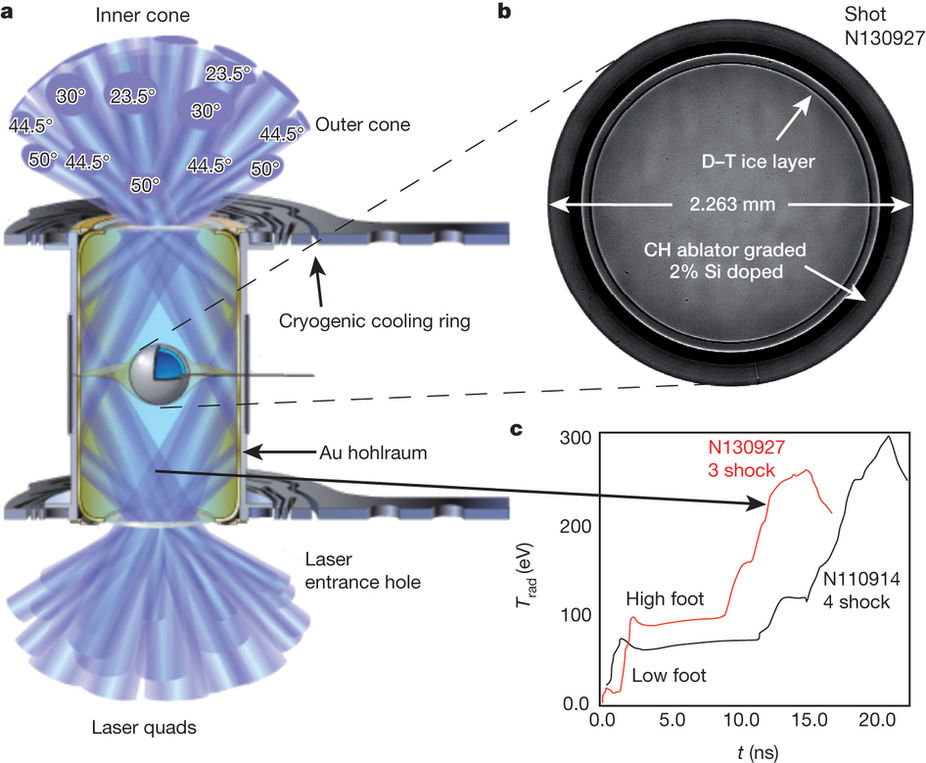
\includegraphics[width=\linewidth]{hohlraum.jpg}
    \caption[Hohlraum design for indirect drive in Inertial Confinement Fusion.]{\textbf{a} Cross-section of the National Ignition Facility's ICF target design showing the gold hohlraum and plastic capsule, fuel pellet, and incident laser bundles. \textbf{b} X-ray image of the actual capsule for N130927 with DT fuel layer and surrounding CH (carbon–hydrogen) plastic ablator. \textbf{c} X-ray radiation drive temperature as a function of time for the National Ignition Campaign (NIC) low-foot implosion and the post-NIC high-foot implosion. Image taken from \cite{hohlraum}.}
    \label{f:hohlraum}
\end{figure}

Overall, the table is unrepresentative of potential operating environments in large-scale power stations, but sets lower limits on the demands of the materials involved in both mainstream proposals for fusion energy production.

\subsection{Effects of radiation on reactor materials}
\label{ss:rad_effect_mat}

\subsubsection{Radiation Damage}
\label{sss:rad_damage}

One of the bigger problems in radiation damage research is the lack of a truly standardised way of measuring damage on materials \cite{srimisbad}. The most common unit is displacements per atom (dpa) \cite{dpa}. It is defined as the average number of displacements undergone by each atom in a material as a result of being irradiated. The fundamental unit of measurement for this, is the number of displacements per unit volume per unit time, $R$
\begin{align}\label{eq:dpa}
    R & = N\int _{E_{\rvar{min}}}^{E_{\rvar{max}}}\int _{T_{\rvar{min}}}^{T_{\rvar{max}}}\phi (E)\,\sigma (E,T)\,\upsilon (T)\;\rvar{d}T\;\rvar{d}E\,,
\end{align}
where $ N $ is the atom number density (no. of atoms per unit volume); $ E $ the incoming particle's energy; $ T $ the energy transferred in a collision of a particle of energy $E$ and a lattice atom; $ \phi(E) $ the energy-dependent particle flux; $ \sigma(E,T) $ the cross-section for the collision of a particle with energy $ E $ resulting in a transfer of energy $ T $ to the struck atom; and $ \upsilon(T) $ the number of displacements per primary knock on atom as a function of transferred energy $ T $. DPA can be calculated by na\"{i}vely multiplying $ R $ by the sample volume and total exposure time (or use fluence, $\Phi(E)$, rather than flux). This ignores the fact that $\sigma (E,T)$ and $\upsilon (T)$ will be locally perturbed in the neighbourhood of damage cascades, but since the bulk volume is much greater than that of the damage cascades', the functions are assumed to remain globally unchanged.

In principle, this is a rather good measure of damage \cite{dpa}. The catch is that, generalised, analytical expressions for $ \sigma(E,T) $ and $ \upsilon(T) $ depend on a slew of parameters and are therefore incredibly hard, if not impossible to derive. That said, they can be discretised and roughly approximated via Monte Carlo (MC) approaches \cite{srim, srimisbad, dpa}. However, damage cascade modelling falls squarely in the realm of pico- to nanosecond timescales, and as such is only tractable with Molecular Dynamics (MD) and Kinetic Monte Carlo (KMC) \cite{dmg_cascade1, dmg_cascade2} approaches. At the end of such cascades, we are often left with dislocation sources or prismatic dislocation loops \cite{dmg_cascade_dln}. Such loops can be used as inputs for Dislocation Dynamics (DD) simulations, which can explore greater temporal and spatial scales \cite{fusmat1s}.

\subsubsection{Transmutation}
\label{sss:transmutation}

Transmutation products are one of the biggest sources of problems for materials in fusion applications \cite{fusmat1, mats_fusion1}. Not only do they tend to embrittle materials, they often also reduce their thermal conductivity \cite{transmute}. The former presents significant challenges for structural materials \cite{ods_rad_res}; the latter is especially egregious for energy extraction by limiting the divertor's ability to conduct heat, thus lowering the reactor's efficiency and causing thermal stresses due to the generation of hot spots that cannot be easily dissipated. As a result, understanding the mechanical and thermal behaviour of transmutation alloys is crucial for moving forward \cite{nirrhard, colcas, hardening}, but doing so requires knowledge of the time evolution of a reactor's components. Since the chemical composition changes in a non-trivial way, so do the mechanical properties. Worse still are the long timescales over which this occurs---on the order of years or tens of years \cite{transmute2}. Even if we were able to experimentally irradiate fusion-relevant materials with appropriately energetic neutrons, it would take years before we could characterise their behaviour, and doing so would be problematic due to radioactive decay.

The way we go about addressing the time-dependent compositional change of a material is to model it. Culham Centre for Fusion Energy's (CCFE), FISPACT \cite{fispact}, takes an MC approach at calculating transmutation and decay products of a sample given certain conditions. The code utilises external data provided by the European Activation File, which provides cross-section and decay rate data for a wide range of isotopes \cite{fispact_library}. Unfortunately, there is a lack of cross-section data for certain neutron energies that contribute in a non-negligible manner to a fusion environment. Interpolating to fill the gaps would not be appropriate as the data is non-smooth and subject to resonance peaks, so the solution is imperfect.

Transmutation products will always be problematic, but they are a fact of working with fusion-relevant materials. Fortunately, there are ways in which inclusions may be modelled via DD (\cref{sss:inclusions}). DD may also be used to model dislocation movement and interaction within heterogeneous media (\cref{ss:multiphase}) as is the case for oxide-dispersion-strengthened (ODS) steels; and transmutation alloys of Tungsten divertors, where Osmium, Rhenium and Tantalum clusters which prove highly problematic for its temperature conductivity and structural integrity \cite{w_cluster1, nirrprop, nirpropmic, nirrmic, ionirrmic, ionirrprop, ionirrprop2}.

\section{Parallel computing}
\label{s:parallel_comp}

Modern processing chips are made up of billions of transistors acting as switches in logic gates. Each time a logic gate fires, the capacitors inside them charge and discharge at the chip's frequency otherwise known as clock speed \cite{cpu_trnstor}. Consider the power of any electronic component,
\begin{align}\label{eq:pow_ec}
    P(t) & = I(t) V(t) \,,
\end{align}
where $ I $ is current and $ V $ is voltage, both as functions of time, $t$. The current, $ I $, of a capacitor and the definition of power, $ P $, as functions of time, $ t $, as well as the definition of capacitance are given by,
\begin{align}\label{eq:cap_cur_pow_dt}
    I(t) = C \dfrac{\mathrm{d}V(t)}{\rvar{d}t} \,, \qquad
    P(t) = \dfrac{\rvar{d}E(t)}{\rvar{d}t}\,, \qquad
    C = \dfrac{Q_\rvar{c}}{V_\rvar{c}}
\end{align}
where $ C $ is capacitance, $ E $ the energy stored in the capacitor, $Q_\rvar{c}$ the charge stored in the capacitor and $V_\rvar{c}$ the voltage of the capacitor. Substituting \cref{eq:cap_cur_pow_dt} into \cref{eq:pow_ec} and integrating twice, we obtain the expression for the energy stored in a capacitor,
\begin{subequations}
    \begin{align}\label{eq:e_cap}
        \int\limits_{0}^{E_{c}}\int\limits_{0}^{\infty} \dfrac{\rvar{d}E(t)}{\rvar{d}t}\; \rvar{d} t & = C \int\limits_{0}^{V_{c}}\int\limits_{0}^{\infty} V(t) \dfrac{\mathrm{d}V(t)}{\rvar{d}t}\; \rvar{d} t\,, \\
        E_{\rvar{c}}                                                                                 & = \dfrac{C V_{\rvar{c}}^{2}}{2}  = \dfrac{Q_\rvar{c} V_\rvar{c}}{2} = \dfrac{Q_\rvar{c}^2}{2C}\,,
    \end{align}
\end{subequations}
where $ V_{\rvar{c}} $, $ E_{\rvar{c}} $, $Q_\rvar{c}$ are the voltage, energy and charge stored in the capacitor. Recalling that in a processing chip, the capacitors are charged and discharged at the chip's clock speed $ f $, we arrive at the expression for power consumption, $ P_{\rvar{c}} $, of a capacitor charging and discharging at frequency $ f $ \cite{microelec},
\begin{align}
    P_{\rvar{c}} & = E_{\rvar{c}} f \propto C V_{\rvar{c}}^{2} f \label{eq:p_cap}\,.
\end{align}

Computer chips are rather more complicated, but their power consumption (also known as power dissipation) is described by a simple addition of terms \cite{cpu_pow},
\begin{align}
    P = P_{\rvar{dyn}} + P_{\rvar{sc}} + P_{\rvar{leak}}\,,
\end{align}
where $ P_{\rvar{dyn}} $ is the dynamic power dissipation given by \cref{eq:p_cap}. The two other dissipation mechanisms are:
\begin{enumerate}
    \item $P_{\rvar{sc}}$, short-circuit, which depends on frequency and occurs when a direct path from transistor to ground is made as a result of multiple transistors conducting simultaneously; and
    \item $P_{\rvar{leak}}$, leakage, which depends on the voltage and is due to micro-currents that form at the p-n junctions\footnote{The p-n junction is the region between the doped semiconductor with free holes, (p-type semiconductor), and the doped semicondutor with free electrons (n-type semiconductor).} of the transistor.
\end{enumerate}
Furthermore, higher voltages and frequencies result in higher temperatures, which in turn mean decreased transistor performance and increased capacitance. The overall result is an energy expenditure curve similar to \cref{f:cpu_en_cnvx} \cite{cpu_en_cnvx} for every processor unit.
\begin{figure}[t]
    \centering
    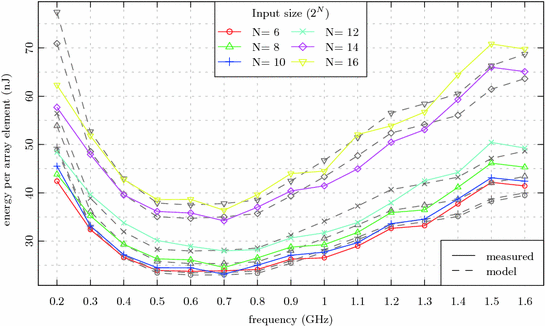
\includegraphics[width=\linewidth]{cpu_en_cnvx.png}
    \caption[Energy expenditure of CPU vs Voltage.]{Energy required by a Samsung Galaxy S2 CPU at \SI{37}{\degreeCelsius} to complete the Gold-Rader implementation of the \emph{bit-reverse} algorithm. The dashed lines denote a theoretical model, image and model from \cite{cpu_en_cnvx}.}
    \label{f:cpu_en_cnvx}
\end{figure}

This set of optimum conditions is the reason behind the multicore and multithreaded design of modern Central Processing Units (CPUs) and Graphics Processing Units (GPUs). It is also why in recent years there has been such a massive push for parallelism in all computing markets. It is simply not feasible to continually increase clock speeds and voltages because cooling solutions would struggle to remove heat fast enough, and power consumption would skyrocket.

\subsection{Computation on graphics processing units}
\label{sc:compgpu}

\begin{figure}
    \centering
    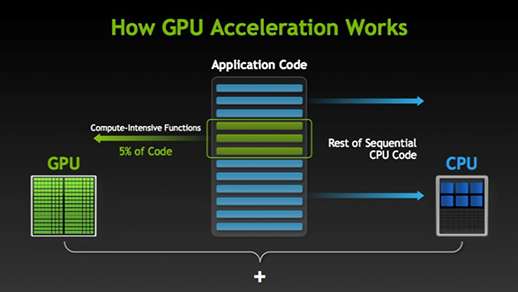
\includegraphics[width=\linewidth]{gpu_parallel.png}
    \caption[CUDA runtime schematic.]{CUDA runtime schematic. Repetitive but computationally intensive tasks can be offloaded to the GPU. Both GPU and CPU are completely indipendent from each other and can work on different parts of the code at the same time, care must be taken to ensure proper syncronisation. Image taken from \cite{nvidia}.}
    \label{f:cuda}
\end{figure}

Central Processing Units (CPUs) are designed not only to perform mathematical operations but logical ones that control program flow. They are tailored to perform the wide variety of operations required by an operating system. These include program scheduling (instruction priorisation, load balancing), instantiation (program loading, unloading, loops, recusion instances) \& branching (if/case statements, go to's), memory operations (fetching, storing, allocation), input/output (IO), and program monitoring (program counters, recursion counters). Modern CPUs have a degree of parallelism and asyncronicity that allows them to increase their total throughput while keeping their operation within near optimal conditions. They are commonly divided into cores and threads, though certain high-end chips have an additional layer named hyperthreading \cite{cpu_arch}.

Given the limited scope of the first computers, the general purpose of CPUs was enough to cover their needs. However, with the advent of personal computers, the demands on CPUs drastically increased. For industrial users these revolved around data acquisition, filtering and preprocessing \cite{fpga, preproc, filtering}. On the other hand, the domestic market demanded ever-increasing levels of abstraction and usability in the form of Graphical User Interfaces (GUIs) such as windows, cursors and sound effects which originally acted as a replacement for haptic feedback. Manufacturers identified this need and moved to provide specialised modules for such tasks. This freed CPU resources and improved user experience by accelerating different processes through hardware means \cite{gpu1, gpu2, gpu3, sound}. These modules include Sound Cards (SCs), Field Programmable Gate Arrays (FPGAs), Graphics Processing Units (GPUs), Application Specific Integrated Circuits (ASICs), Cryptographic Accelerators, Regular Rxpression (RegEx) Accelerators, among others. These external pieces of specialised hardware are collectively dubbed \emph{hardware accelerators}.

Graphics Processing Units were originally intended to offload the very data-intensive but computationally simple operations needed for 3D gaming and rendering \cite{gpu1, gpu2, gpu3}. Graphics processing was a prime candidate for hardware acceleration because the operations on each pixel are largely the same across the screen. Due to their original purpose as gaming and rendering accelerators, they were never designed to operate on higher than single precision data. In fact, single precision (32-bit precision) is still good enough to encode 32-bit colour depth (8-bit channel per RGB colour + 8-bit alpha channel), which only the most high-end monitors support \cite{monitor}. It is also worth noting that because the same operations apply to different pieces of (mostly) independent data, they can all be performed at the same time, often trivially reducing the order of polynomial complexity algorithms. For example, an $\mathcal{O}(N)$ process can be reduced to $\mathcal{O}(1)$ if all $N$ instances fit in a single parallel execution and are independent of one another.

As previously mentioned, GPU parallelism frees up enormous amounts of CPU processing power that can be put to good use running other programs or performing complementary serial processes, while the GPU works concurrently on its dataset. Parallelism has been used by the scientific community for years, but the focus has mainly been on CPU parallelism \cite{cpu_par}. Consequently, its scope was lagerly limited to the use of computational clusters. The two main reasons for this were the fact that GPUs lacked support for higher precision arithmetic, and the very limited to non-existent support for scientific computing in languages such as OpenGL \cite{gpu_comp}.

It wasn't until the development of the OpenCL and OpenACC standards that GPUs caught the attanetion of the scientific community as a viable way of exploiting parallelisation without access to a computing cluster.

OpenCL allows one to work with heteragoenous systems and is similar to C in that it's very low level. It works on a wide range of hardware accelerators and is therefore useful for many scientific and engineering applications, but it's also relatively hard to use. One can make use of libraries written in OpenCL to facilitate development, but it is still a fully fledged C-type language \cite{opencl}.

OpenACC is similar to OpenMP in that they both use pragmas\footnote{Pragmas are especially formated comments that specific compilers recognise and turn into special instructions at compile time. They are not part of the programming language's official standard, but rather compiler-specific extensions. Pragmas are usually programmed in C or Assembly and must be implemented by the compiler manufacturer. Nothing prevents application developers from writing the would-be pragma's code directly into their application, but this can prove a lengthy and difficult process. The rigid nature of pragmas, as well as the compiler manufacturer's priorities, limit their scope and usability.} and they both work in shared memory environments---same GPU and same CPU respectively. This is no coincidence as OpenACC was designed as an extension of OpenMP for developing parallel applications on hardware accelerators. Unfortunately, being pragma based, the standard requires significant work by compiler manufacturers, so its adoption has therefore been slow \cite{openacc}. Furthermore, despite simplifying development and minimising the barrier to entry, the use of pragmas limits the flexibility and adaptability of the framework compared to OpenCL.

Recently however, a third option has become viable. NVidia's Computer Unified Device Architecture (CUDA) framework provides the best aspects of both OpenCL and OpenACC. The tradeoff is that it only works on NVidia GPUs and is a closed source product. However, the accessibility and flexibility of CUDA provides anyone familiar with C/C++ the means to develop a GPU application with little issue. NVidia is also strongly backing scientific research by adding double precision support to their GPUs. They have also worked to provide parallel equivalents of well known serial libraries---such as cuBLAS \& cuFFT---for scientific computing. They have additionally developed a wide range of specialist graphics cards tailor-made for scientific purposes. As such, they are the leaders in GPU computing in scientific communities \cite{nvidia}.

\subsubsection{Hurdles for parallelisation}
\label{sc:hurdpara}

\begin{figure}
    \centering
    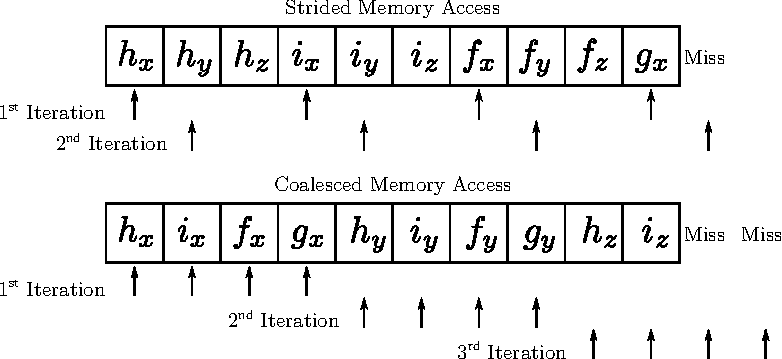
\includegraphics[width=\linewidth]{mem_access.pdf}
    \caption[Memory access pattern example.]{Arrows represent fetch requests by single threads in a GPU. Data should be arranged in such a way that all threads in a warp (collections of 32 threads) can simultaneously access contiguous memory locations, reducing cache-misses and improving throughput. This access pattern can be unintuitive when parallelising serial algorithms, but is extremely important, especially when using scientific computing cards, as they are optimised for long computation times and low memory fetch frequency.}
    \label{f:mem_accessIntro}
\end{figure}

The difficulty in parallelisation varies tremendously from problem to problem. Problems where data is uncorrelated and independent---such as sampling well-behaved probability distributions---are almost trivially parallelisable. Problems where data is correlated or strongly dependent on its neighbours---such as Dislocation Dynamics---require a more careful approach \cite{parallel_algs}.

The largest hurdle when implementing parallel algorithms is often the efficient use of data. In order to obtain good parallel performance, a lot of thought has to be placed on data access patterns, data read/write conflicts, and memory allocation and transfer \cite{nvidia}. For best performance, all this must be analysed on a case by case basis. If done incorrectly, the performance of a parallel application may be lower than the serial version. One must consider a wide range of parameters to successfully parallelise a problem. Among these are GPU architecture, problem size, computational and memory complexity, code branching, required arithmetic precision, and error tolerances \cite{nvidia, gpu_rev}.

Efficient parallelisation of many problems requires \emph{coalesced memory access} as shown in \cref{f:mem_accessIntro}, which means we have to be extremely careful when mapping CPU memory to global GPU (device) memory. The fact that threads work ``simultaneously''\footnote{Not quite but essentially simultaneously. See \cite{nvidia} for details.} means that in order to obtain good performance, data which is to be simultaneously loaded into each thread must be contiguous. This maximises cache memory use and therefore reduces slow memory fetch operations.

Special cases, such as having a parallel dislocation line segment to a surface, as discussed in \cref{ss:analytic_forces}, must be treated carefully due to the way code branching works in GPUs. There are various ways of doing so:
\begin{inparaenum}[\itshape 1\upshape)]
    \item if the special case is inexpensive, it can be treated within the same GPU function;
    \item if the special case is expensive and always known (such as certain boundary conditions in FEM), it can be placed in its own GPU function that treats it separately;
    \item if the special case is expesive and only found at runtime, it may be asynchronously treated by the CPU or buffered into its own GPU function to be executed at a later time.
\end{inparaenum}

\begin{figure}
    \centering
    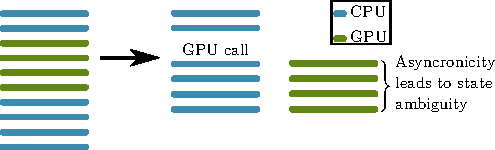
\includegraphics[width=\linewidth]{async.pdf}
    \caption[GPU and CPU asynchronous execution.]{GPU and CPU code run independent of each other. This can lead to state ambiguities if both sides need to be aware of one another \cite{nvidia}.}
    \label{f:async_gpu_cpu}
\end{figure}
One of the advantages of GPU-CPU independence is that both can work concurrently on different aspects of the problem. If both systems have to talk to each other, or there are any race conditions (one process needs to finish before the other can start), then one must tread carefully, ensuring proper syncronisation and data mapping before proceeding (see \cref{f:async_gpu_cpu}).

The reason why code branching is bad for GPU parallelisation is down to the fact that they work like software-customisable vector machines. As in vector processors, collections of threads all carry out the same operation on different pieces of data at the same time. The threads essentially behave as one, operating on different data. This is advantageous to a GPU because it means more energy and space can be used for computation rather than logic and scheduling. However, this eliminates the ability for code to branch within each collection of threads. This means that every branch of an \texttt{if} or \texttt{switch-case} statement will be executed whether a condition is met or not\footnote{If the branch can be resolved at compile time, it is possible for the compiler to prune it as part of compile time optimisation. However, this can be unreliable and depends on how transparent the optimsation is to the compiler, how agressive the optimisation setting is, and how the compiler is implemented. Therefore, relying on compile time optimisation to prune branches is not recommended.}. Only data storage depends on whether a condition is true or false, as illustrated in \cref{f:code_branching}.
\begin{figure}
    \centering
    \begin{subfigure}[t]{0.48\linewidth}
        \centering
        \begin{minted}{c}
if (y == 0){
    x = a+b;
}
else if (y == 1){
    x = a*b;
}
else{
    x = a/b;
}
			\end{minted}
        \caption{CPU code will only execute if the condition is met. This is called code branching.}
    \end{subfigure}
    ~
    \begin{subfigure}[t]{0.48\linewidth}
        \centering
        \begin{minted}{cuda}
p = (y == 0);
p: x = a+b;

p = (y == 1);
p: x = a*b;


!p: x = a/b;
			\end{minted}
        \vspace{12pt}
        \caption{GPU code executes every line but only stores results if the flag before the colon is true.}
    \end{subfigure}
    \caption[Explanation of warp divergence.]{The NVidia CUDA compiler replaces \texttt{if} and \texttt{case} statements with logical flags \texttt{p}. Every line is executed, but the data is only stored if the flag prior to the colon is true \cite{nvidia}. This means that having rare but computationally expensive special cases will tank parallel performance and must therefore be dealt with separately.}
    \label{f:code_branching}
\end{figure}

Dislocation Dynamics (DD)---in particular 3D Discrete Dislocation Dynamics (3D DDD)---can greatly benefit from parallelisation, especially when coupling to Finite Element Methods (FEM). It is worth noting that there are potential issues arising from the very computationally expensive functions and special cases that often arise from analytical solutions in 3D DDD. There are also potential issues with data redundancy---which are non-limiting in the short term---that may eventually require a more data-efficient approach as the computational capabilities and data capabilities of GPUs converge. \Cref{ss:parallel_ddd} expands on these issues in the context of DD.

\section{3D dislocation dynamics modelling}
\label{s:3d_ddd}

The plastic deformation of materials is generally governed by the generation and motion of line defects known as dislocations through the crystal lattice. Microstructural features such as grain boundaries, precipitates and inclusions impede dislocation motion causing strengthening but often limiting ductility \cite{init_fail_dln}. Understanding the behaviour of the dislocation ensemble is highly complicated even when ignoring dislocation-microstructure interactions. However, if we want to truly comprehend their real-world behaviour, we cannot limit ourselves to idealised scenarios.

One of the most often used parametrisations of DD is Discrete Dislocation Dynamics (DDD). Where dislocations are parametrised as a series of nodes linked by straight line segments. This reduces computational requirements and allows for analytic solutions to be obtained. At present, neither DDD nor Finite Element (FE) models can truly handle all the complexities of real-world alloys \cite{ddd_fem1, paradis, fem_ddd2, fem_ddd}. For one, DDD relies on assuming a linear-elastic isotropic solid domain with periodic or infinite boundary conditions, while FE relies on assuming continuum properties inside a \emph{finite} domain.

Crystal Plasticity Finite Element Methods (CPFEM) use constitutive equations to calculate dislocation motion and generation on a set of slip systems. These are given as dislocation densities and thus can still be considered ``bulk'' models because there are no explicit dislocations interacting with one another \cite{cpfem1}. CPFEM can handle finite strains and anisotropy but not strain localisation/slip bands, etc.

Furthermore, dislocations often accumulate in the vicinity of microstructural features. The interaction of dislocations with microstructure and other dislocations can lead to work hardening and local stress concentrations that can lead to failure initiation \cite{size_effects, dln_ind_hard}. Hardware accleration, i.e. using Graphics Processing Units (GPUs), has been shown to be very effective in DDD \cite{gpu_ddd}, and has the potential to enable the simulation of much larger numbers of dislocations for longer timescales. In order to study these phenomena we must find a way of coupling DDD and FEM into a single multiscale model with the potential to simulate micromechanical tests more accurately than CPFEM. With a model such as this, we may potentially be able to predict and observe emergent phenomena/properties, explain michromechanical behaviours, and even predict and explain experimental results based on underlying dislocation mechanisms\footnote{Though predicting and replicating experimental results requires the initial conditions of the experiment and simulation be roughly equivalent.}.

\subsection{Coupling dislocation dynamics to finite element methods}
\label{ss:ddd_fem}

Coupling dislocation dynamics (DD) to FEM is important to properly simulate micromechanical tests because DD provides us with a more precise set of inputs and greater granularity for solving the FE problem. There are at present two methods with which to do so, the \nameref{sss:superposition} and the \nameref{sss:discrete_continuum}. Discrete dislocation dynamics, where the dislocation is broken into nodes connected by segments is a relatively compuationally- and data-efficient implementation of dislocation dynamics, which has the added advantage of having analytical solutions for straight-line segments. However, as discussed in \cref{sss:lvl_set}, explicit discretisation is not the only way to tackle the problem.

\subsubsection{Superposition Method}
\label{sss:superposition}

\begin{figure}
    \centering
    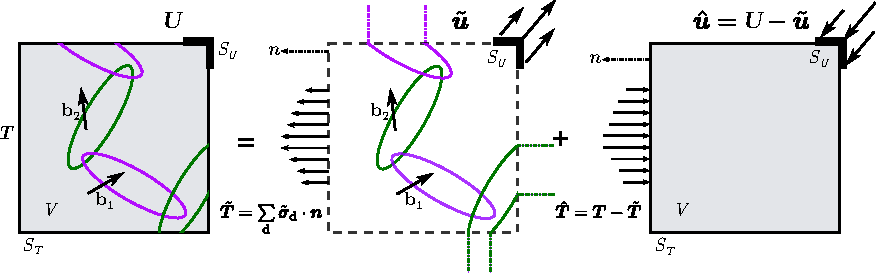
\includegraphics[width=\linewidth]{fem_ddd.pdf}
    \caption[Superposition Method for DDD-FEM coupling.]{The superposition used to couple DDD and FEM. The volume $V$ is bounded by a surface $S = S_{T} \cup S_{U}$ and contains a dislocation ensemble and is subjected to tractions $\vec{T}$ on $S_{T}$ and $\vec{U}$ on $S_{u}$. First, the traction, $\vec{\tilde{T}}$, and displacement, $\vec{\tilde{u}}$, fields due to the dislocations in the infinite domain (DDD) are evaluated on the boundaries $S_{T}$ and $S_{U}$ respectively. Then an elastic boundary value problem can be solved with FEM to calculate the corrective elastic fields required to satisfy the boundary conditions $\vec{\hat{T}} = \vec{T} - \vec{\tilde{T}}$ and $\vec{\hat{u}} = \vec{U} - \vec{\tilde{u}}$.}
    \label{f:fem_ddd}
\end{figure}

The Superposition Method (SM) works by decomposing the problem into separate DDD and FE problems (\cref{f:fem_ddd}). It is assumed that a linear-elastic body $ V $ bounded by a surface $ S $ is subject to traction boundary conditions, $ \vec{T} $, on $ S_{T} $ and displacement boundary conditions, $ \vec{U} $, on $ S_{u} $. The formulation proposed in \cite{dismot} to impose traction-displacement boundary conditions on DDD problems in finite domains states that the total displacement and stress fields can be written as a superposition of displacement and stress fields obtained from DDD and FE,
\begin{subequations}
    \label{eq:superposition}
    \begin{align}
        \vec{U}      & = \vec{\tilde{u}} + \vec{\hat{u}}\,,            \\
        \tns{\sigma} & = \tns{\tilde{\sigma}} + \tns{\hat{\sigma}}\, .
    \end{align}
\end{subequations}
The, (\textasciitilde), fields are those associated with the dislocation in an infinite medium and are obtained by evaluating analytic fields in a DDD simulation. The corrective, (\textasciicircum), fields are those which must be superimposed to ensure the boundary conditions are met. This means that the image fields can be obtained by running a FE simulation with the ``corrected'' displacement and traction fields,
\begin{subequations}
    \begin{align}
        \vec{\hat{u}}                    & = \vec{U} - \vec{\tilde{u}}\,,                                                                                 \\
        \tns{\hat{\sigma}} \cdot \vec{n} & = \vec{\hat{T}} = \vec{T} - \underbrace{\vec{\tilde{T}}}_{\displaystyle{\tns{\tilde{\sigma}}}\cdot \vec{n}}\,,
    \end{align}
\end{subequations}
where $ \vec{n} $ is the outer unit normal vector to $ S $. As a dislocation segment moves closer to the surface, its (\textasciitilde) field diverges and starts causing numerical problems \cite{bdd}. \Cref{ss:paperIntro} is a more in-depth discussion on the superposition method and dislocation-induced surface tractions.

A further problem with this method is that modelling elastic inclusions not only requires the calculation of forces induced by dislocations on the inclusion's surface, but also demands the calculation of so-called polarisation stresses due to differences in the inclusion's and matrix elastic properties \cite{dismot, bdd, ddd_precip}.

That said, the relative simplicity of the superposition method has made it a popular choice \cite{analytic_tractions, ddd_fem_sm, ddd_fem_sm2} for coupling DDD and FEM because all it requires is the calculation of forces and displacements on the boundaries (see \cref{ss:analytic_forces}).

\subsubsection{Discrete Continuum Method}
\label{sss:discrete_continuum}

The Discrete Continuum Method (DCM) takes an alternative approach to solving the same coupling problem. The DCM only treats short-range dislocation-dislocation interactions analytically while all other interactions are numerically calculated via FEM \cite{dcm}. It is based on the regularisation of the atomic displacement jump across the slip plane into a plastic strain inclusion according to eigenstrain theory \cite{eigenstrain}. Like the Superposition Method, the DCM also assumes the simulated volume to be linear-elastic.

The eigenstrain formalism assumes that material defects can be represented as stress-free strain distributions, dubbed \emph{eigenstrains} \cite{eigenstrain}. For example, a dislocation loop of any shape may be approximately represented by thin, coherent, plate-like inclusions with the same contour as the loop and a characteristic thickness, $ h $, as shown in \cref{f:eigenstrain} \cite{dcm}. The eigenstrain tensor, $ \tns{\varepsilon^{\rvar{p}}} $, can then be defined as a symmetric dyadic product of the Burgers vector, $ \vec{b} $, and slip plane normal $ \vec{n} $,
\begin{align}\label{eq:eigenstrain}
    \tns{\varepsilon^{\rvar{p}}} & \equiv \dfrac{1}{2h} (\vec{b} \otimes \vec{n} + \vec{n} \otimes \vec{b})\,.
\end{align}
\Cref{eq:eigenstrain} can be used to calculate approximate elastic fields from the stress-free eigenstrain distribution. The approximation is accurate far from the dislocation core \cite{dln_core}. As we move closer---but still outside the core region---the approximation tends toward the exact discrete dislocation solution as $ h \to 0$. From linear elasticity, the total plastic strain is the sum of the individual plastic strains due to each dislocation segment.
\begin{figure}
    \centering
    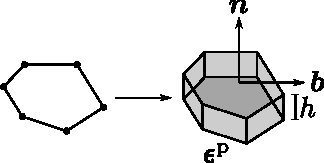
\includegraphics[width=0.5\linewidth]{eigenstrain.pdf}
    \caption[The eigenstrain formalism.]{The eigenstrain formalism as defined in \cite{eigenstrain}. The dislocation is being approximated by a thin coherent inclusion of thickness $ h $, whose strain-free stress tensor $ \tns{\sigma^{\rvar{p}}} $ as defined by \cref{eq:eigenstrain}. The vectors $ \vec{n} $ and $ \vec{b} $ are the normal vector to the slip plane and the dislocation line's Burgers vector.}
    \label{f:eigenstrain}
\end{figure}

The formalism then lets us solve the boundary value problem by finding the stress tensor $ \tns{\sigma} $, elastic strain $ \tns{\epsilon^{\rvar{e}}} $ and displacement $ \vec{u} $ in mechanical equilibrium with the boundary conditions and plastic strain distribution $ \tns{\epsilon^{\rvar{p}}} $ from the ``inclusions''.

It is worth noting that in order to accurately calculate the eigenstrains, there must be sufficient FE nodes inside the thin plate. Therefore, smaller values of $ h $ necessitate finer FE meshes. Furthermore, the original DCM experienced numerical blow up as dislocation-dislocation distances approached $ h $ \cite{dcm0}, but this has since been addressed. Assuming linear-elasticity, the revised model \cite{dcm} yields,
\begin{subequations}\label{eq:discrete_continuum}
    \begin{align}
        \nabla \cdot \tns{\sigma} + \vec{f} = \vec{0} \quad & \in V \setminus \{A\}\,, \\
        \tns{\sigma} = \tns{E} : \tns{\epsilon} \quad       & \in V \setminus \{A\}\,, \\
        [[\vec{u}]] \quad                                   & \rvar{across } \{A\}\,,  \\
        \vec{u} = \vec{u_{0}} \quad                         & \in S_{U}\,,             \\
        \tns{\sigma} \cdot \vec{n} = \vec{T} \quad          & \in S_{T}\,.
    \end{align}
\end{subequations}
At time $ t $, $ \{A\} $ denotes the area swept by the dislocation loops since the start of the simulation. $ [[\vec{u}]] $ denotes displacement jumps tangent to $ \{A\} $ due to dislocation glide; its magnitude and direction depend on the Burgers vector $ \vec{b} $. $ \tns{E} $ is the 4\textsuperscript{th}-order elasticity tensor, $ \tns{\sigma} $ the small strain tensor, $ \vec{f} $ are the body forces and, $ : $, is the double dot product defined as, $ (\tns{E}:\tns{\epsilon})_{ij} = E_{ijkl}\epsilon_{kl} $, between a rank 4 tensor ($ \tns{E} $) and a rank 2 tensor ($ \tns{\epsilon} $). The operator, $ \setminus $, is the set difference defined as, $ A \setminus B = \{x \in A | x \notin B\} $. \Cref{eq:discrete_continuum} can then be linearly decomposed three parts which are solved via FEM or DDD and coupled as described in \cite{dcm}.

It is worth noting that the DCM is \emph{substantially} more complicated than the SM. By requiring the finite elements be small enough for the eigenstate formalism to work, it strongly couples DDD to the FE model and software implementation. It shifts the brunt of the computational workload from DDD to FEM. Essentially trading computationally intensive, long-range interactions which scale on the order of $ \mathcal{O}(N^{2}) $, where $ N $ is the number of dislocation line segments; for computationally intensive tasks scaling on the order of $ \mathcal{O}(M^{3}) $ where $ M $ is the number of finite elements in 3D (assuming linear cubic elements). Furthermore, it cannot be used with BE methods as the eigenstrain formalism demands the use of internal elements rather than simply requiring a surface mesh.

That said, the DCM allows for reductions in the computational complexity of certain parts of the problem which would otherwise have to be done via DDD \cite{dcm}; namely long-range dislocation-dislocation or dislocation-surface interactions via an interaction distance cutoff that is only possible with the eigenstrain formulation. Compared to the superposition method, gains in computational efficiency grow as dislocation density increases with respect to the number of finite elements. Since dislocation-dislocation and dislocation-surface interactions are among the most computationally expensive aspects of DDD, the DCM can reduce the overall computational cost of simulations with large enough dislocation densities and fine enough finite element meshes.

\subsubsection{Level set method}
\label{sss:lvl_set}

Even though the level set method has not strictly been used to couple DD to FEM, it has been used to model inclusions \cite{ddd_inclusion_as_force}, as described in \cref{sss:inclusions}. This type of dislocation dynamics is fundamentally distinct from DDD because Level Set DD uses arbitrary functions rather than a discretisation approach to represent dislocations lines. The idea is that in 3D, a dislocation $ \gamma(t) $ can be represented by the intersection of two zero levels of two level set functions (see \cref{f:lvl_set_dd}),
\begin{subequations}\label{eq:lvl_set}
    \begin{align}
        \phi(x(t),y(t),z(t),t)                                                          & = 0\,, & \qquad
        \psi(x(t),y(t),z(t),t)                                                          & = 0\,,          \\
        \dfrac{\rvar{d} \phi}{\rvar{dt}} = \partial_{t}\phi + \vec{v} \cdot \nabla \phi & = 0\,, & \qquad
        \dfrac{\rvar{d} \psi}{\rvar{dt}} = \partial_{t}\psi + \vec{v} \cdot \nabla \psi & = 0\,,
    \end{align}
\end{subequations}
where $ \vec{v} $ is the dislocation velocity. This definition uses the material derivative because it is assumed that the function and its spatial coordinates are all functions of time, $ t $. The material derivative also comes up when deriving the Navier-Stokes equations of fluid dynamics.
\begin{figure}
    \centering
    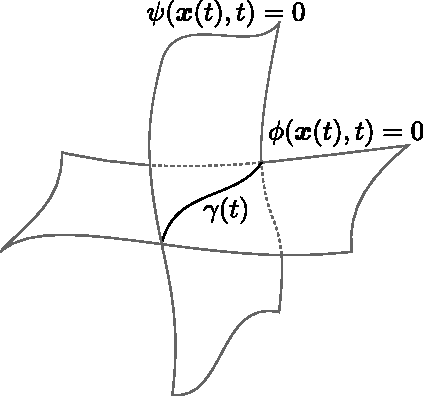
\includegraphics[width=0.3\linewidth]{level_set.pdf}
    \caption[Level set Dislocation Dynamics.]{Diagram of a continuous dislocation $ \gamma(t) $ as the intersection of the zero level of two level set functions $ \phi(\vec{x}(t),t),~\psi(\vec{x}(t),t) $ as posed by \cref{eq:lvl_set}. Image edited from \cite{lvl_set_dd}.}
    \label{f:lvl_set_dd}
\end{figure}

The level set method is significantly more computationally expensive than DDD \cite{lvl_set_dd}. It must solve two coupled quasi-linear partial differential equations whose character is in general undefined. It therefore requires the use of very robust numerical solvers such as higher order Total Variation Deminishing (TVD) Runge-Kutta methods for time discretisation (TVD-RK4 or higher), and high order ENO (Essentially Nonoscillatory $ \mathcal{O}(N^5) $ or higher) or WENO (Weighted Essentially Non-Oscilatory) interpolation methods for spatial discretisation \cite{lvl_set_ddd_inc} for the solutions to converge satisfactorily. The method also makes it impossible to use many of the useful analytical solutions one can find by discretising dislocations into straight line segments. Another problem is that this method has never been truly coupled to the finite element method. However, if one were to do so there are two naïve ways of going about it:
\begin{inparaenum}[\itshape1\upshape)]
    \item numerically integrating along the dislocation lines and finding a way to numerically calculate the forces on FE nodes, or
    \item discretising the level set curves and using either the DCM or SM to find forces and displacements.
\end{inparaenum}
The former would be very computationally expensive. Furthermore, no one has found a way to compute the forces or displacements exerted by generally shaped, non-discretised dislocations, numerical solutions are possible as they are needed to find self-interaction energies and dislocation-dislocation forces \cite{lvl_set_dd} but general, closed-form analytical ones are most likely impossible to find. Both approaches defeat the purpose of the level set method, necessitating some form of discretisation whilst keeping the high computational cost. As a result of this, the level set method is not nearly as popular as DDD utilising either the SM or DCM.

\subsection{Non-singular continuum theory of dislocations}
\label{ss:non-singular_dln}

The Peach-Koehler formula describes the fundamental interactions of dislocations \cite{pk_force} according to the force, $ \vec{f} $, that a local stress $ \tns{\sigma} $ exerts on a unit length of dislocation line with Burgers vector, $ \vec{b} $, and line direction, $ \vec{\xi} $,
\begin{align}
    \vec{f} & = (\tns{\sigma} \cdot \vec{b}) \times \vec{\xi}\,.
\end{align}

The internal stress field of a dislocation loop in a homogenous, infinite, linear-elastic medium is given by the contour integral around a loop $ L $ \cite{mura_t},
\begin{align}\label{eq:field_stress}
    \sigma_{ij}^{\infty}(\vec{x}) & = C_{ijkl} \oint_{L} \epsilon_{lnh} C_{pqmn} \dfrac{\partial G_{kp}(\vec{x} - \vec{x'})}{\partial x_{q}} b_{m}\; \rvar{d}x'_{h}\,,
\end{align}
where $ C_{ijkl} $ is the elastic stiffness tensor, $ \epsilon_{lnh} $ the permutation operator, $ \vec{b} $ the Burgers vector, and $ G_{kp}(\vec{x} - \vec{x'}) $ is Green's function of elasticity \cite{mura_t}. $ G_{kp}(\vec{x} - \vec{x'}) $ is defined as the displacement component in the $ x_{k} $ direction at point $ \vec{x} $ in response to a unit point force applied in the $ x_{p} $ direction at point $ \vec{x'} $ \cite{a_non-singular_continuum_theory_of_dislocations}. In an isotropic elastic solid, $ G(\vec{x} - \vec{x'}) $, takes the form,
\begin{align}\label{eq:elastic_green_func}
    G_{ij}(\vec{x} - \vec{x'}) & = \dfrac{1}{8\pi \mu}\left[ \delta_{ij} \partial_{pp} - \dfrac{1}{2(1-\nu)} \partial_{ij} \right] R(\vec{x} - \vec{x'})\,,
\end{align}
where $ \mu $, $ \nu $ are the isotropic shear modulus and Poisson's ratio respectively, $ \delta_{ij} $ is the Kronecker Delta, $ \partial_{x_{1} \ldots\, x_{n}} \equiv \dfrac{\partial^{n}}{\partial x_{1} \ldots\, \partial x_{n}}$, and $ R = \lVert \vec{x} - \vec{x'} \rVert $. However, considering that $ \vec{x} \to \vec{x'} \Rightarrow R \to 0 \Rightarrow \partial_{i} R \to \infty $, some (or all) components of the stress field diverge. Furthermore, the total elastic energy also diverges,
\begin{align}\label{eq:e_dln1}
    E & = \dfrac{1}{2} \int S_{ijkl} \sigma_{ij}(\vec{x}) \sigma_{kl}(\vec{x})\; \rvar{d}^{3}\vec{x}\,,
\end{align}
where $ S = C^{-1} $ is the elastic compliance tensor. These divergent properties prove problematic when numerically computing dislocation forces and energies. \Cref{eq:e_dln1} can also be expressed as a double line integral \cite{dewit1, dewit2},
\begin{align}\label{eq:e_dln2}
    E = & - \dfrac{\mu}{8\pi} \oiint_{L} \partial_{k} \partial_{k} R(\vec{x}-\vec{x}') b_{i} b'_{j} \;\rvar{d}x_{i} \;\rvar{d}x'_{j}\nn
        & - \dfrac{\mu}{4 \pi (1-\nu)} \oiint_{L} \partial_{i} \partial_{j} R(\vec{x}-\vec{x}') b_{i} b'_{j} \;\rvar{d}x_{k} \;\rvar{d}x'_{k}\nn
        & + \dfrac{\mu}{4 \pi (1-\nu)} \oiint_{L} \partial_{k} \partial_{k} R(\vec{x}-\vec{x}') b_{i} b'_{i} \;\rvar{d}x_{j} \;\rvar{d}x'_{j}\nn
        & - \nu \oiint_{L} \partial_{k} \partial_{k} R(\vec{x}-\vec{x}') b_{i} b'_{j} \;\rvar{d}x_{j} \;\rvar{d}x'_{i}\;,
\end{align}
which is important when describing how \citet{a_non-singular_continuum_theory_of_dislocations} derived their non-singular expression.

The singularity in $ R $ is the result of unreasonably and unphysically assuming a dislocation loop's Burgers vector distribution is a Delta function. The assumption was made to allow for closed-form and relatively simple expressions. As noted in \cite{bv_dist}, other distributions may be used but they either result in significantly more complicated expressions or destroy the analytical nature of the classical formulation.

There have been many attempts at removing this singularity, including finite-strain elasticity \cite{non_sing3}, non-local and gradient elasticity \cite{non_sing1, non_sing2}, interaction cut-off radius \cite{pk_force}, average stress at two points on opposite sides of the dislocation line \cite{non_sing4, non_sing5}, and spreading the Burgers vector distribution out over a finite width \cite{bv_dist, non_sing6, non_sing7}. Unfortunately all of these approaches failed in one way or another \cite{a_non-singular_continuum_theory_of_dislocations}. Depending on the approach, various undesirable qualities may present themselves, including
\begin{inparaenum}[\itshape1\upshape)]
    \item inconsistencies with other theories;
    \item impractical implementation;
    \item lack of closed-form solutions for non-straight finite dislocations;
    \item lack of self-consistency; and
    \item the possibility for multiple non-degenerate expressions and solutions for the line integral of the dislocation line energy.
\end{inparaenum}

\Citet{a_non-singular_continuum_theory_of_dislocations} defined and justified a different Burgers vector distribution that maintains the mathematical convenience of the classical formulation and eliminates such an unphysical assumption. They did so by introducing a Burgers vector density function,
\begin{subequations}\label{eq:b_dist}
    \begin{align}
        \vec{b}          & = \int \vec{g}(\vec{x}) \;\rvar{d}^{3} \vec{x}\label{seq:bv_dist}\,, \\
        \vec{g}(\vec{x}) & = \vec{b} \tilde{w}(\vec{x}) = \vec{b} \tilde{w}(r)\,,
    \end{align}
\end{subequations}
where $ r \equiv \lVert \vec{x} \rVert $. When substituting \cref{seq:bv_dist} into \cref{eq:field_stress,eq:e_dln2}. The result of multiplying $ R $ with components of $ \vec{b} $ results in the following integrals,
\begin{subequations}\label{eq:r_times_b_dist}
    \begin{align}
        R(\vec{x} - \vec{x}') b_{m}        & = \int R(\vec{x} - \vec{x}'') g_{m}(\vec{x}'' - \vec{x}') \;\rvar{d}^{3}\vec{x}''\,,                                                          \\
        R(\vec{x} - \vec{x}') b_{m} b'_{n} & = \iint R(\vec{x}'' - \vec{x}''') g_{m}(\vec{x} - \vec{x}'') g_{n}(\vec{x}''' - \vec{x}') \;\rvar{d}^{3}\vec{x}'' \;\rvar{d}^{3}\vec{x}'''\,.
    \end{align}
\end{subequations}
Using \cref{eq:b_dist,eq:r_times_b_dist} as guidelines, they defined the following convolutions,
\begin{subequations}
    \begin{align}
        w(\vec{x}) & \equiv \tilde{w}(\vec{x}) * \tilde{w}(\vec{x}) = \int \tilde{w}(\vec{x}-\vec{x}')\tilde{w}(\vec{x}')\; \rvar{d}^{3} \vec{x}'\,, \\
        R_{a}      & \equiv R(\vec{x}) * w(\vec{x}) = \int R(\vec{x} - \vec{x}') w(\vec{x}') \;\rvar{d}^{3} \vec{x}'\,.
    \end{align}
\end{subequations}
At which point they assumed there exists an integrable function $ w(\vec{x}) $ such that
\begin{align}
    R_{a} = \sqrt{R(\vec{x})^{2} + a^{2}} = \sqrt{x^{2} + y^{2} + z^{2} + a^{2}}\,,
\end{align}
where $ a $ is an arbitrary constant meant to represent the dislocation core radius, whose value may be estimated from atomistic simulations. This is essentially a definition that can be used to replace $ R $ in the classical equations and eliminate the singularity by including a free parameter. However, in order to ensure this is mathematically sound, there must indeed exist a function which yields $ R_{a} $ as \citet{a_non-singular_continuum_theory_of_dislocations} defined it. This can be done by making use of the following property for the convolution of two suitably differentiable functions, $ \partial_{i} (f*g) = \partial_{i}f * g = f * \partial_{i} g $. We may take the Laplacian twice,
\begin{subequations}
    \begin{align}
        \nabla^{2}[\nabla^{2} \{R(\vec{x}) * w(\vec{x})\} ] & = \nabla^{2}[\nabla^{2} R_{a}(\vec{x})]\,,                                                             \\
        \nabla^{2}[\nabla^{2} \{R(\vec{x})\}] * w(\vec{x})  & = \nabla^{2}[\nabla^{2} R_{a}(\vec{x})]\,,                                                             \\
        \nabla^{2}[\nabla^{2} \{R(\vec{x})\}]               & = \nabla^{2}\left[\dfrac{2}{R}\right] = -8\pi \delta^{3}(\vec{x}) \label{eq:hand_wavy}\,,              \\
        \nabla^{2}[\nabla^{2} R_{a}(\vec{x})]               & = \nabla^{2}\left[\dfrac{2}{R_{a}} + \dfrac{a^{2}}{R_{a}^{3}}\right] = -\dfrac{15 a^{4}}{R_{a}^{7}}\,, \\
        w(\vec{x})                                          & = \dfrac{15 a^{4}}{8\pi R_{a}^{7}} \label{eq:dist}\,.
    \end{align}
\end{subequations}
\Cref{eq:hand_wavy} is a very brave statement given that,
\begin{align}
    \nabla^{2} \left[R^{-1}\right] & = \nabla^{2}\left[(x^{2} + y^{2} + z^{2})^{-1/2}\right] = 0\,,
\end{align}
everywhere except when $x^2 + y^2 + z^2 = 0$, where the expression is equal to $-0/0$. If we want the equation to be solveable, it is necessary to define an infinitesimally small sphere with radius 0, whose surface area is $4\pi\delta^3(\vec{x})$, multiplying by $-2$ (negative sign from $-0/0$, and 2 from the numerator of \cref{eq:hand_wavy}) yields $-8\pi\delta^3(\vec{x})$. \Cref{eq:dist} is a similarly dubious statement that can be justified by noting that,
\begin{align}
    \lim\limits_{a\to 0} w(\vec{x}) = \delta^{3}(\vec{x})\,.
\end{align}
Nevertheless, the non-singular formulation by \citet{a_non-singular_continuum_theory_of_dislocations} fixes the physically and mathematically problematic assumption that Burgers vectors follow 3D Dirac delta distributions, and proves useful in producing analytical expressions (see \cref{ss:analytic_forces}) that are not much more complex than the singular case.

\subsection{Analytical forces exerted by a dislocation line segment on surface elements}
\label{ss:analytic_forces}

Whether using the SM or DCM, coupling DDD to FEM requires the traction field $ \tns{\sigma^{\infty}}(\vec{x}) \cdot \vec{n}(\vec{x}) $ to be distributed among the set of relevant discrete nodes of a FE or BE model. In the DCM model this applies to dislocations that are sufficiently close to the boundary; while in the SM, it applies to all dislocations.
Regardless of the coupling model, the force exerted by a dislocation ensemble on a node $ n $ on element $ e $ is given by,
\begin{align}\label{eq:ddd_fem_force_intro}
    \vec{F}^{(n)} = \int_{S_{e}} \left[\tns{\sigma^{\infty}}(\vec{x}) \cdot \vec{n}(\vec{x})\right] N_{n}(\vec{x})\; \rvar{d}S_{e}\,,
\end{align}
where $ \rvar{d}S_{e} $ is the infinitesimal surface element with surface area $ S_{e} $. $ N_{n}(\vec{x}) $ are so-called shape functions (interpolation functions) that distribute the traction field among the surface element's nodes.

The problematic singularity associated with the classical Volterra dislocation is avoided by using the non-singular formulation of \citet{a_non-singular_continuum_theory_of_dislocations} discussed in \cref{ss:non-singular_dln}, which changes \cref{eq:elastic_green_func} into \cref{eq:ns_elastic_green_func},
\begin{align}\label{eq:ns_elastic_green_func}
    G_{ij}(\vec{x} - \vec{x'}) & = \dfrac{1}{8\pi \mu}\left[ \delta_{ij} \partial_{pp} - \dfrac{1}{2(1-\nu)} \partial_{ij} \right] R_{a}(\vec{x} - \vec{x'})\,.
\end{align}

Using the non-singular definition of $ G(\vec{x}-\vec{x}') $ in \cref{eq:field_stress} we obtain the expression for the stress field of a single straight dislocation line segment bounded by two dislocation nodes at $\vec{x_1}$ and $\vec{x_2}$ \cite{a_non-singular_continuum_theory_of_dislocations},
\begin{align}
    \label{eq:stressIntro}
    \tns{\tilde{\sigma}}(\vec{x}) = &
    - \dfrac{\mu}{8\pi} \int\limits_{\vec{x_1}}^{\vec{x_2}} \left( \dfrac{2}{R_{a}^{3}} + \dfrac{3a^2}{R_{a}^{5}} \right) \left[ \left(\vec{R} \times \vec{b}\right) \otimes \mathrm{d}\vec{x'} + \mathrm{d}\vec{x'} \otimes \left(\vec{R} \times \vec{b}\right) \right]          \\
    %
                                    & + \dfrac{\mu}{4\pi(1-\nu)} \int\limits_{\vec{x_1}}^{\vec{x_2}} \left( \dfrac{1}{R_{a}^{3}} + \dfrac{3a^2}{R_{a}^{5}} \right) \left[ \left(\vec{R} \times \vec{b}\right) \cdot \mathrm{d}\vec{x'} \right]\vec{I_2}\nonumber                  \\
    %
                                    & -\dfrac{\mu}{4\pi(1-\nu)} \int\limits_{\vec{x_1}}^{\vec{x_2}}  \dfrac{1}{R_{a}^{3}} \left[ \left(\vec{b} \times \mathrm{d}\vec{x'}\right) \otimes \vec{R} + \vec{R} \otimes \left(\vec{b} \times \mathrm{d}\vec{x'}\right) \right]\nonumber \\
    %
                                    & + \dfrac{\mu}{4\pi(1-\nu)} \int\limits_{\vec{x_1}}^{\vec{x_2}} \dfrac{3}{R_{a}^{5}} \left[ \left(\vec{R} \times \vec{b}\right) \cdot \mathrm{d}\vec{x'} \right]\vec{R}\otimes\vec{R}\nonumber,
\end{align}
where,
\begin{align}
    \vec{R}            & = \vec{x} - \vec{x'} = y \vec{l} + r \vec{p} + s \vec{q} \\
    %
    R_a                & = \sqrt{\vec{R} \cdot \vec{R} + a^2}                     \\
    %
    \mathrm{d}\vec{x'} & = -\mathrm{d} y \vec{l}\,.
\end{align}
The vectors $\vec{p}$ and $\vec{q}$ are aligned with the edges of the rectangular finite element, $\vec{n} = \vec{p} \times \vec{q}$ is the element surface normal (pointing away from the dislocation), and $\vec{l}$ is parallel to the dislocation line segment as shown in \cref{f:force_lin_rect}. Then (provided $\vec{l}$ is not parallel to $\vec{p}$ or $\vec{q}$) $\vec{R}$ can be expressed in terms of $(\vec{l},~\vec{p},~\vec{q})$ with coefficients,
\begin{align}
    y = \dfrac{\vec{R}\cdot \vec{n}}{\vec{l}\cdot \vec{n}} \label{eq:problemIntro},\quad
    %
    r = \dfrac{\vec{R}\cdot (\vec{q} \times \vec{l})}{\vec{p}\cdot (\vec{q} \times \vec{l})}, \quad
    %
    s = \dfrac{\vec{R}\cdot (\vec{p} \times \vec{l})}{\vec{q}\cdot (\vec{p} \times \vec{l})}\,.
\end{align}
\Cref{eq:stressIntro} can be turned into a series of triple integrals solved via recursion relations and a few seed functions.

\Cref{f:force_lin_rectIntro} diagramatically summarises the over 40 triple line integrals needed to find an analytical expression of the nodal forces on linear rectangular elements.
\begin{figure}
    \centering
    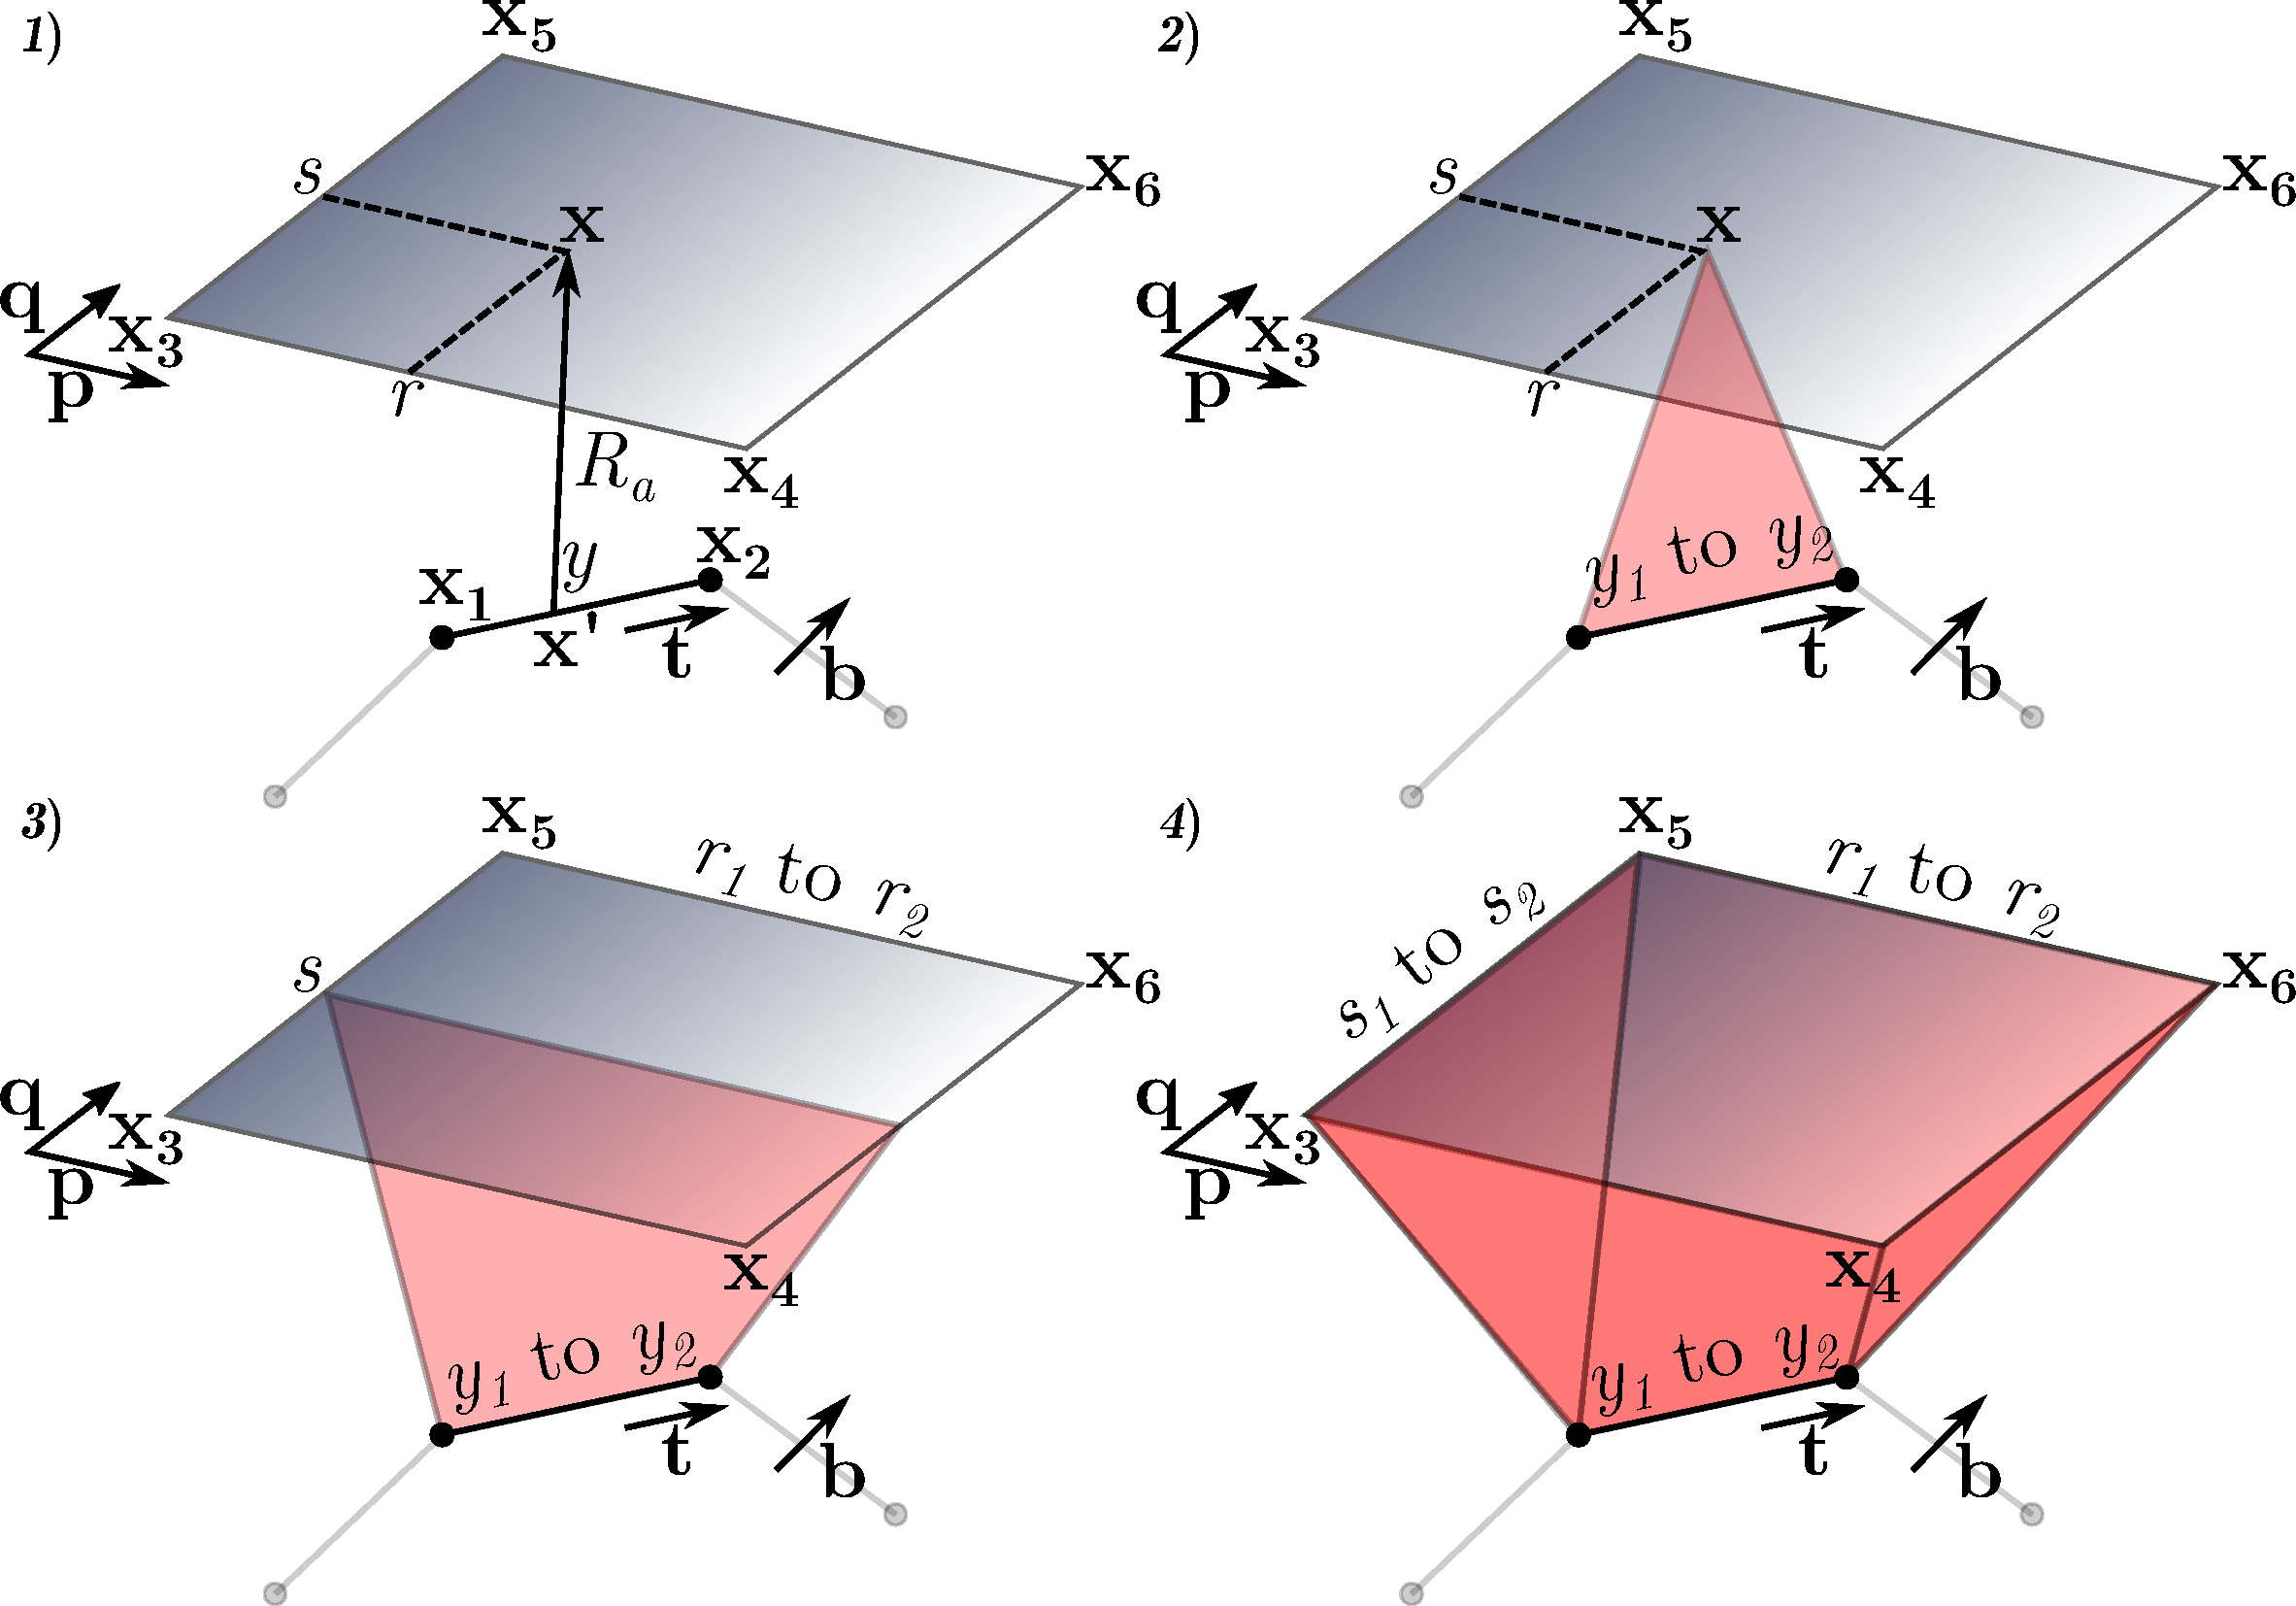
\includegraphics[width=0.8\linewidth]{force_calc_linear_rectangle.pdf}
    \caption[Analytic tractions on linear rectangular surface elements.]{Diagram of the parametric line integrals solved by \citet{analytic_tractions} to find the forces on linear rectangular surface elements.}
    \label{f:force_lin_rectIntro}
\end{figure}
\Cref{c:tractions} contains more detail regarding the theory, implementation and advantages of these analytic tractions over the traditional solution of using Gauss quadrature.

\subsection{Multiphase simulations}
\label{ss:multiphase}

Modelling heterogeneity in DDD remains challenging. The core assumption of DDD is that we have a homogenous linear elastic solid with invariant properties. However, modelling multiphase systems such as multicrystals and inclusions necessitates a weakening of such assumptions, particularly the solid's homogeneity. Multiphase models are also necessary to apply DDD to more realistic scenarios.

Fusion in particular is riddled with examples of highly heterogenous materials. As previously mentioned, neutron bombardment often causes clustering of transmutation products, particularly on divertor and first wall materials; such clusters often substantially change many of their mechanical and thermal properties. The whole point of Oxide-Dispersion Strengthened (ODS) steels \cite{ddd_ods} is to hamper radiation damage by distributing oxide inclusions within their matrix; if we hope to model such alloys with DDD we must find a way to relax our homogeneity criteria.

Furthermore, many potential candidates for structural and even first wall materials of fusion reactors are designed with complex microstructures in order to resist thermal creep and radiation damage. Understanding dislocation behaviours near the crystal boundaries of these microstructurally complex materials is another niche where DDD simulations can shed light into the mechanisms that give rise to these materials' desirable properties.

\subsubsection{Polycrystalline materials}
\label{ss:polycrystal}

Polycrystalline materials have been studied using DDD, however most of these are in 2D. One of the easiest phenomena to investigate with 2D DDD are grain size effects \cite{2d_pcm, 2d_pcm2}.

It is well known that much of the grain size strengthening effects arise from dislocation-grain boundary (GB) interactions including transmission, reflection, emission and absorption of dislocations \cite{grain_size_eff1, grain_size_eff2}; with transmission being the most typically observed.

These models depend on the grain boundary energy density, $ E_{\rvar{GB}}(\delta\theta) $, where $ \delta\theta $ is the crystallographic misorientation between neighbouring crystals; resolved shear stress, $ \tau $, on the incoming dislocation with Burgers vector $ \vec{b_{1}} $; critical penetration stress for the GB, $ \tau_{\rvar{GB}} $; and Burgers vector of the dislocation debris, $ \vec{\Delta b} = \vec{b_{1}} - \vec{b_{2}} $, left behind when the incoming dislocation, $ \vec{b_{1}} $, transmits throught the grain boundary to become a dislocation with Burgers vector, $ \vec{b_{2}} $. The relationship may be approximated by,
\begin{align}\label{eq:dln_trns}
    \tau \lvert\vec{b_{1}}\rvert^{2} & \geq \tau_{\rvar{pass}} \lvert\vec{b_{1}}\rvert^{2} = E_{\rvar{GB}}(\theta) \lvert\vec{b_{1}}\rvert + \alpha G \lvert\vec{\Delta b}\rvert^{2}\,,
\end{align}
where $ \alpha $ is the material constant and $ G $ the shear modulus. The grain boundary energy density was proposed by \citet{gb_e_dens} to have the simple form,
\begin{align}
    E_{\rvar{GB}} & = 	\begin{cases}
        k \dfrac{\delta\theta}{\theta_{1}}                 & \quad 0 \leq \delta\theta < \theta_{1}\,,          \\
        k                                                  & \quad \theta_{1} \leq \delta\theta < \theta_{2}\,, \\
        k \dfrac{\pi/2 - \delta\theta}{\pi/2 - \theta_{2}} & \quad \theta_{2} \leq \delta\theta < \pi/2\,,
    \end{cases}
\end{align}
where $ k,~ \theta_{1},~\theta_{2} $, are material specific.

This is of course a gross simplification of the real 3D problem, but this approach was used by \citet{2d_pcm} to investigate the Hall-Petch effect, which correlates grain size with flow stress of a polycrystal,
\begin{align}\label{eq:hall_petch}
    \sigma & = \sigma_{0} + \kappa \left(\dfrac{d_{0}}{d}\right)^{n}\,,
\end{align}
where $ \sigma_{0} $ is the yield stress, $ d_{0} $ a reference crystal size, $ \kappa $ the Hall-Petch slope and $ n $ the crystal size sensitivity parameter. \Citet{2d_pcm} showed that the model reproduces the Hall-Petch effect quite successfully. As a consequence, they showed that even what might appear as an overly simplistic approach can describe a complex emergent phenomenon such as the Hall-Petch effect.

Aside from the Hall-Petch effect, the model has also been utilised by \citet{2d_pcm2} to study the thickness effects of three different types of polycrystalline thin films:
\begin{inparaenum}[\itshape 1\upshape )]
    \item no surface treatment,
    \item surface passivation layer, and
    \item surface grain refinement zones.
\end{inparaenum}
In their study, Frank-Reed sources were seeded across the domain, and the superposition principle was utilised to calculate displacement, strain and stresses in the thin films. Their results qualitatively reproduced experimental observations from expected dislocation patterns, stress distributions, and the eventual disappearance of the size effect as the films got thicker.

Though two-dimensional models might seem useless, they have their place, particularly when thin films are concerned. However, they may also be of use when investigating the effects of dislocations on the mechanical behaviour of superconducting tape---whose applications range from medical imaging to fusion energy production. The exotic composition and crystallography of many superconductors (perovskites) would make 3D models very complex and computationally expensive, so 2D models may offer viable alternatives. On top of this, a superconducting tape's operating environment would often have it under strains which might not strictly lie in-plane, but given a small enough segment of tape, strains orthogonal to its plane may be neglected. Thus making 2D models an acceptable first attempt at tacking the problem, at least until developments in 3D models make more realistic studies of such complex systems possible.

The 3D case is substantially more complicated than the 2D case. A study by \citet{twinning}, looked at the role of twinning on the hardening response of polycrystalline Mg using 3D DDD. The article is a perfect example of why 3D DDD is so much more complex than 2D DDD. Admitedly, it uses a material with a HCP crystal structure, whose mobility laws are substantially more complex than those of FCC or BCC materials.

In 3D DDD one must account for dislocation-twin boundary (TB) interactions. These may be obtained via geometric considerations, MD, and experimental evidence \cite{twinning2,twinning3,twinning4,twinning5}. We must have information regarding how dislocations are transmitted through a TB such as
\begin{inparaenum}[\itshape 1\upshape)]
    \item whether a dislocation leaves a residual dislocation on the TB,
    \item the possible pre-TB and post-TB slip planes a dislocation can be transmitted to,
    \item which loading conditions are conducive to which transmission behaviour and
    \item which types of dislocation can be transmitted or reflected and in what ways \cite{twinning}.
\end{inparaenum}
All this obviously depends on the twinning plane, so in order to study more realistic scenarios one must have all the necessary knowledge to properly account for all dislocation-TB interactions. Furthermore, it is possible that certain dislocations may leave behind twinning dislocations that end up as TB steps, whose movement can lead to TB migration and twin growth \cite{twinning6, twinning7}.

\Citet{twinning} modelled four scenarios in order to deconvolve the effects that twins and grain boundaries have on the mechanical behaviour of a cube-shaped crystal. They modelled
\begin{inparaenum}[\itshape 1\upshape)]
    \item a twinned polycrystal with two TBs and GBs on the edges of the cube,
    \item a single crystal with no TBs or GBs,
    \item a polycrystal with no TBs but GBs,
    \item a twinned crystal with TBs but not GBs.
\end{inparaenum}
It is worth noting that the effects of twin growth in plasticity were not accounted for in their DDD simulation and instead had to be numerically computed via the hardening rate $ \theta $,
\begin{subequations}
    \begin{align}
        \theta             & = \dfrac{\rvar{d}\sigma}{\rvar{d}\epsilon} = \dfrac{\rvar{d}}{\rvar{d}\epsilon}  \left[E\left(\epsilon - \epsilon_{\rvar{slip}}^{\rvar{p}} - \epsilon_{\rvar{twin}}^{\rvar{p}}\right)\right] = \theta_{\rvar{s}} + \theta_{\rvar{TG}}\,, \\
        \theta_{\rvar{TG}} & = -\dfrac{\rvar{d}}{\rvar{d}\epsilon} \left[E \epsilon_{\rvar{twin}}^{\rvar{p}} \right] = -E \bar{m} \gamma_{\rvar{twin}} \dfrac{\rvar{d}}{\rvar{d} \epsilon} \left[f_{\rvar{twin}}\right]\label{seq:tg}\,,
    \end{align}
\end{subequations}
where $ \theta_{\rvar{TG}} $ is the hardening rate due to twin growth, $ \bar{m} $ the mean Schmid factor of the participating twins $ \gamma_{\rvar{twin}} $ the characteristic twinning shear and $ \dfrac{\rvar{d}}{\rvar{d} \epsilon} \left[f_{\rvar{twin}}\right] $ is the rate of change of the twin volume fraction with respect to the applied strain. These parameters must be empirically obtained.

With their model, \citet{twinning} managed to qualitatively reproduce experimental observations, including the concave shape of strain-stress curves that arises from the competing hardening effect of TBs restricting dislocation motion (\cref{f:twinning}), and the softening produced by twin growth as obtained from \cref{seq:tg}.
\begin{figure}[t]
    \centering
    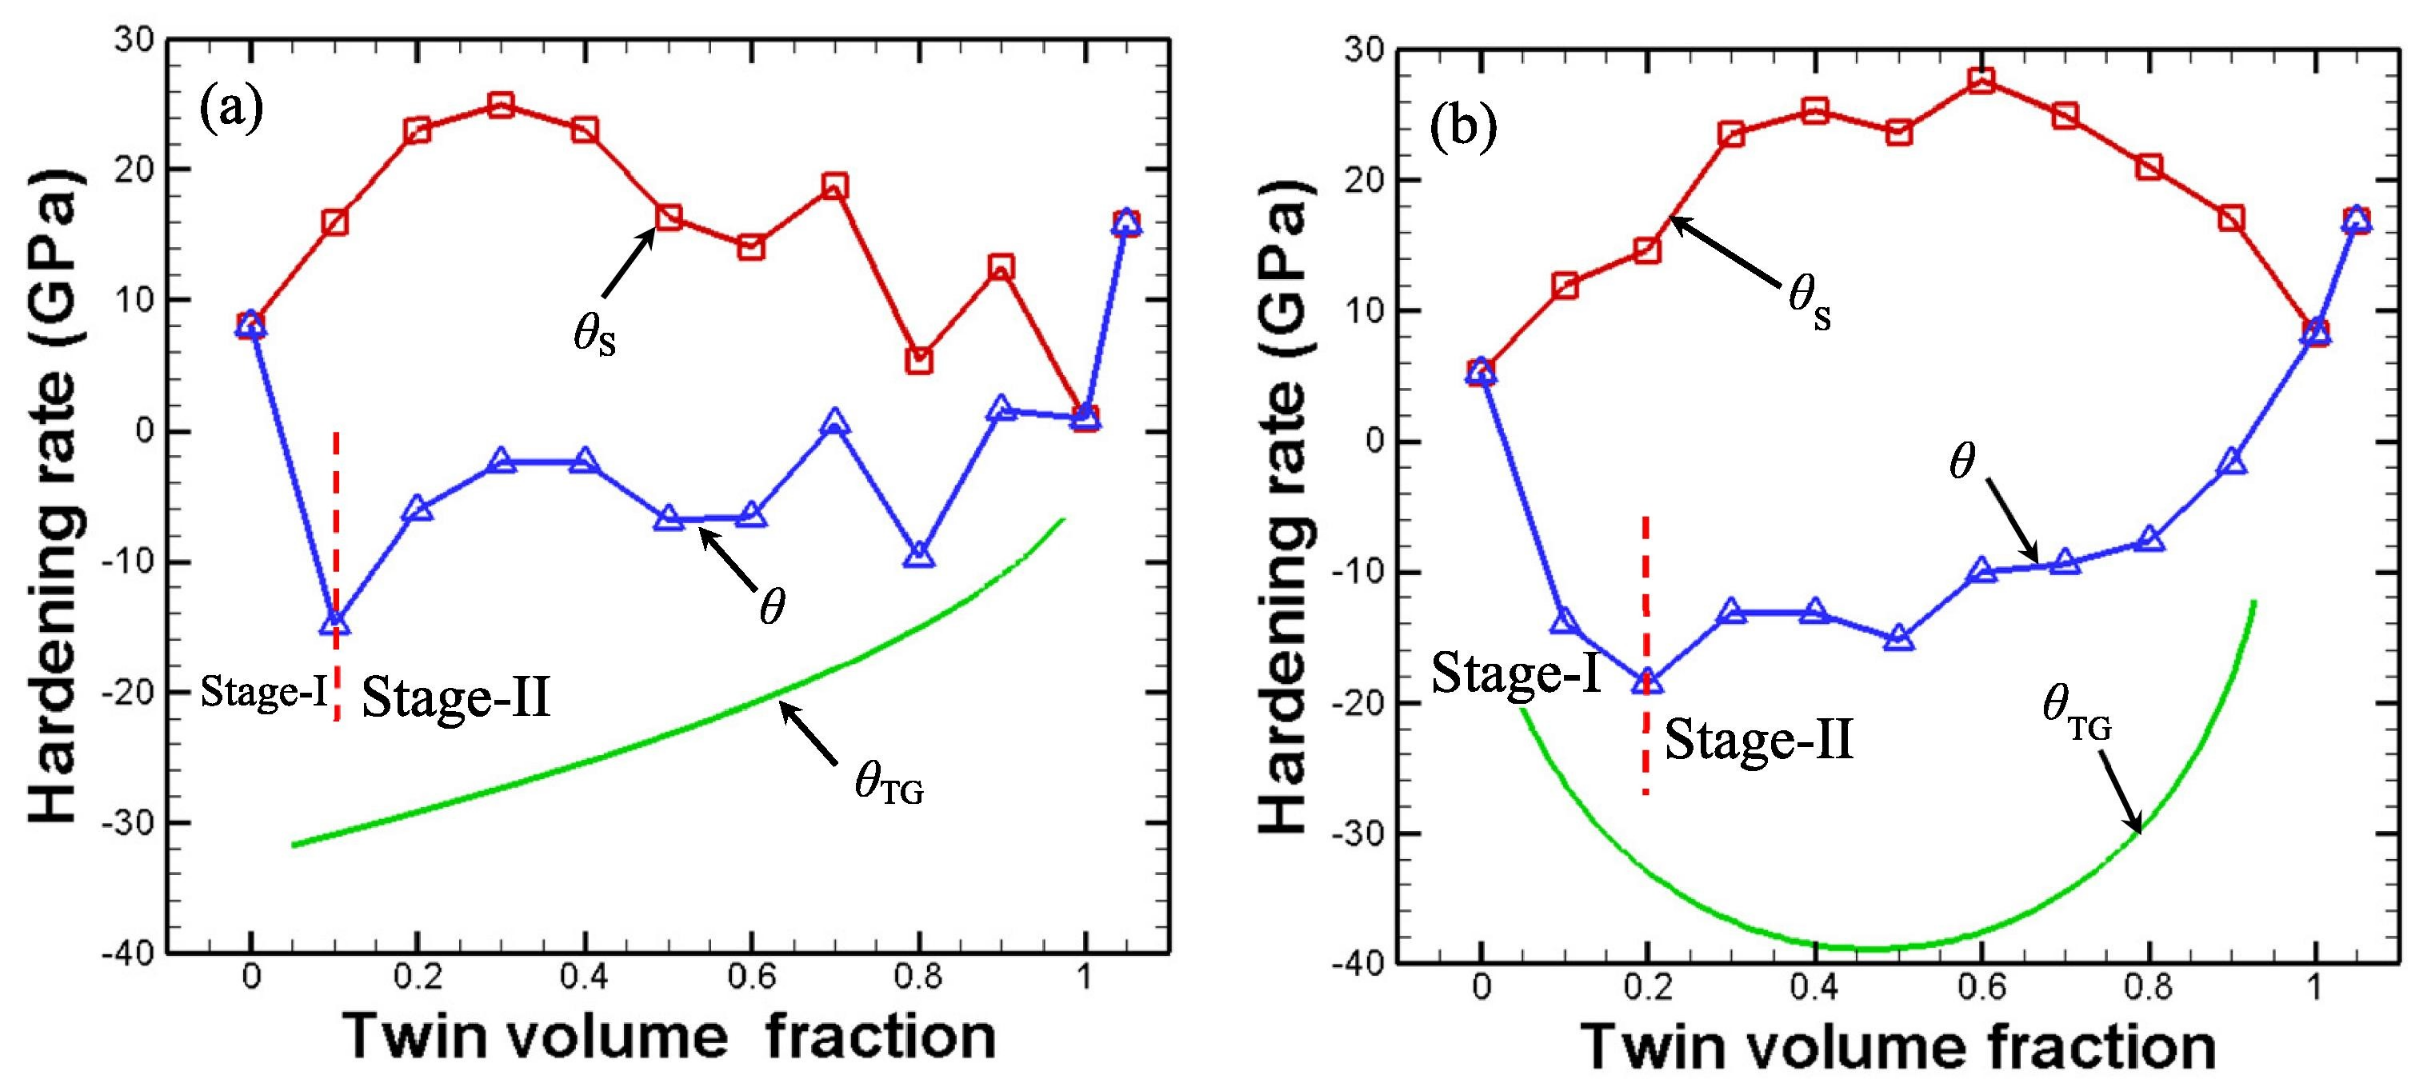
\includegraphics[width=\linewidth]{twinning.png}
    \caption[Modelling twinned multicrystals with DDD.]{Simulated hardening rate as a function of twin volume fraction for (a) yz compressive loading and (b) tensile loading. Image edited from \cite{twinning}.}
    \label{f:twinning}
\end{figure}

Twin boundaries in 3D are analogous to grain boundaries in 2D, given that they are coherent, narrow boundaries rather than messy, often incoherent grain boundaries. Consequently, grain boundaries are much harder to treat in 3D; instead, the community focuses on multiphase models where the details of dislocation transmission between phases are ignored or simplified as expanded upon in \cref{sss:inclusions}.

\subsubsection{Inclusions}
\label{sss:inclusions}

Dislocation-permeable inclusions have been simulated via the SM \cite{sm_incl}. As mentioned in \cref{sss:superposition}, there is a need to calculate polarisation stresses due to differences in the elasticity of both phases. Using the same notation as \cref{sss:superposition} this can be done by breaking up the image stress into,
\begin{subequations}
    \begin{align}\label{eq:sm_pol_stress}
        \tns{\hat{\sigma}} & = \tns{^{\rvar{m}}C} \tns{\hat{\epsilon}} \quad \in V_{\rvar{m}}                                                                                  \\
        \tns{\hat{\sigma}} & = \tns{^{\rvar{p}}C} \tns{\hat{\epsilon}} + \left[\tns{^{\rvar{p}}C} - \tns{^{\rvar{m}}C}\right] \tns{\tilde{\epsilon}} \quad \in V_{\rvar{p}}\,,
    \end{align}
\end{subequations}
where $ \rvar{m},~\rvar{p} $ denote whether a variable belongs to the matrix or precipitate respectively and $ \tns{C} $ is the elastic stiffness tensor.

\Citet{sm_incl} not only modelled a cuboid inclusion, but bimetallic interfaces in 3D. They found that under the right conditions, dislocations can pass from one phase to the other. When a dislocation passes into a different phase, it leaves an antiphase boundary on the slip plane. Therefore, in order for a dislocation to move from one phase to another, it needs excess energy equal to the antiphase boundary (APB) energy of the area it sweeps within the precipitate. This means that as a node passes from one phase to another, it feels a repulsive force $ F_{b} $. The next dislocation moving along the same APB will then feel an attractive force, $ F_{b} $ to dissolve the APB. Once both dislocations move into the new matrix, they form a superdislocation bound by the APB energy \cite{apb}. However, as the dislocation length increases with respect to the precipitate's volume, the production of Orowan loops around it becomes more energetically favourable than moving into the new phase \cite{sm_incl, apb}. Both of these behaviours have been observed when using the superposition method.

The eigenstrain method \cite{eigenstrain_incl} as described in \cref{sss:discrete_continuum} has been shown to be a viable solution to this problem. One can compute the stresses and displacements produced by the dislocation ensemble on the inclusions' surfaces via DCM or SM. The SM method however needs to calculate polarisation stresses \cite{bdd}, an operation that significantly increases the number of calculations necessary to solve the problem.

The DCM method has been used to simulate multiphase materials where the simulated dislocations reproduced experimentally observed behaviours such as the zig-zag patterns and dislocation forests produced by dislocations around precipitates in nickel superalloys \cite{dcm0, dcm_incl}. Reproducing such behaviours is not as trivial as simply adding inclusions to the simulation domain. In order to produce accurate results, one requires knowledge of the coherency stress between the different phases \cite{dcm_incl}. Such stresses are often due to lattice mismatches and differences in the thermal expansion coefficients. These coherency stresses localise the dislocations around the inclusions and are responsible for the observed localisation and aggregation of dislocations around precipitates as seen in \cref{f:coherency} \cite{dcm_incl}.
\begin{figure}[t]
    \centering
    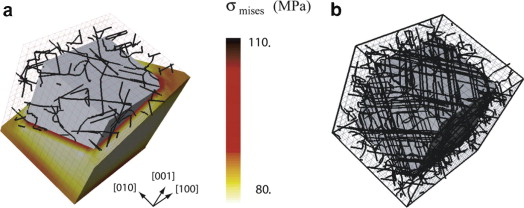
\includegraphics[width=\linewidth]{dln_inclusion.jpg}
    \caption[Modelling dislocation inclusion interactions with the discrete continuum model.]{(a) Shows the initial dislocation configuration after relaxation in the presence of the calculated von Mises coherency stresses $ \tns{\sigma}_{\rvar{mises}} $. (b) Shows the dislocation forresting around the inclusion as a result of 0.2\% plastic strain for the [001] case. Image obtained from \cite{dcm_incl}.}
    \label{f:coherency}
\end{figure}

The level set method has also been successfully used to model inclusions. In contrast to the aforementioned methods, they are assumed to be regions in space where dislocations experience a repelling force, instead of a region in space with distinct characteristics to the matrix. The force profile can be very simply defined to depend on the radial distance from the dislocation to a point in the ``inclusion's'' volume \cite{ddd_inclusion_as_force}. It can also be modulated depending on the nature of the inclusion by making the force a radial function, thus avoiding many of the numerical issues facing DDD-FEM couplings (see \cref{ss:ddd_fem,ss:analytic_forces}). It is also possible to make the inclusions impermeable or semi-permeable depending on the magnitude and steepness of the force gradient, as presented in \cite{ddd_inclusion_as_force}. Arbitrarily shaped inclusions are also possible if one were to also use angular components in the force function, through the use of spherical harmonics and even piecewise-parametric fourier series. This is a simple and versatile method that can be applied to DDD as well.

Though mathematically appealing, such an approach is far from representing the reality of dislocation-inclusion interactions. More realistic scenarios require the use of more commonplace DDD-FEM coupling methods. Implementing arbitrarily-shaped particles is not impossible in DDD---particularly if they can be discretised. Aside from the significantly lower computational requirements of the time evolution and dislocation-dislocation interactions compared to the level set method, one of the biggest advantages of using the SM and DCM methods is that everything, from tractions and displacements on the inclusions, to the coherence stresses on the matrix, can be natively computed from experimentally obtained values. Besides, the method for treating inclusions as functions is still viable. On the other hand, the level set method is so far limited to this approach. Furthermore, if the inclusion is a different crystal or a twin of the same material, as in \cite{twinning}, it is possible to use the DCM or SM to study the transmission of dislocations from one phase to the other; something that is not yet possible with the level set method.

\subsection{Parallelising discrete dislocation dynamics}
\label{ss:parallel_ddd}

It has been shown that DDD lends itself well to parallelisation. \Citet{gpu_ddd} investigated some of the more computationally intensive parts of DDD in DDLab \cite{ddlab}, a freely available DD code for Matlab. The algorithms whose parallel performance was studied in \cite{gpu_ddd} were
\begin{inparaenum}
    \item remote (segment-segment) forces,
    \item surface tractions and
    \item image stresses.
\end{inparaenum}
The remote force computation has $ \mathcal{O}(N^{2}) $ computational complexity, where $ N $ is the number of dislocation segments. The quadratic scaling is due to the $ r^{-1} $ dependence of the dislocation stress fields, so long range interactions cannot be ignored. Both the surface traction and image stress calculations have $ \mathcal{O}(k N) $ computational where $ k $ is the total number of surface nodes and $ N $ the number of dislocation line segments.

As is usually the case in parallel computing, there is often more than one way to parallelise a problem. The optimal strategy depends on the problem itself. It was no different in \cite{gpu_ddd} as shown in \cref{f:gpu_ddd}. \Citet{gpu_ddd} realised that the segment-segment computation can be done via $ \mathcal{O}(N^{2}) $ parallelism, where single pairs of dislocation segments are sent to a single thread, and then globally reduced. However, this approach is $ \mathcal{O}(N^{2}) $ in memory and can lead to inefficient data reuse. So they opted instead for $ \mathcal{O}(N) $ parallelisation and serialisation. In this scheme each thread is assigned a unique segment, and each thread computes the forces between its assigned segment and all the others while serially adding the force contributions. The memory access pattern they found best was that of a serial procedure, the reason is that in-thread calculations are serialised so having coalesced memory access patterns for threads would cause problems when serially accessing data for the calculation.
\begin{figure}[t]
    \centering
    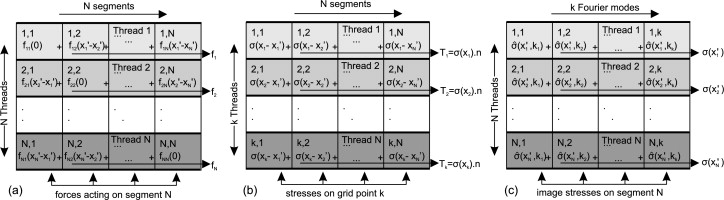
\includegraphics[width=\linewidth]{gpu_ddd.jpg}
    \caption[Parallelisation strategies for three problems in 3D DDD.]{Parallelisation strategies for: (a) the $ N^{2} $ segment interactions; (b) surface traction at k grid points and; (c) and image stresses on $ N $ segments. Image taken from \cite{gpu_ddd}.}
    \label{f:gpu_ddd}
\end{figure}

However, there is another approach \citet{gpu_ddd} did not consider. It combines both of the aforementioned strategies, $ \mathcal{O}(N^{2}) $ memory and $ \mathcal{O}(N) $ parallelisation and serialisation. Such an approach requires two copies of the input data (one per access pattern). One pattern would allow each thread to obtain its uniquely assigned segment in a coalesced manner. The second would be the serial access pattern already present. Thus obtaining the best possible performance at the cost of doubling the required memory. This is a better strategy provided there is enough device memory\footnote{Assuming the line direction is calculated inside the program, each dislocation line segment represents 3, 3-element \texttt{double} precision vectors (8-bytes per entry), totalling 72 bytes in global memory per dislocation line segment (two nodes + Burgers vector per segment). There must also be enough global memory to output the forces, which represent 1, 3-element \texttt{double} precision vector per dislocation node, totalling 24 bytes per node. Assuming a single dislocation loop with $ N $ nodes (therefore $ N $ segments), this brings the total global memory requirement to $ 96N $ bytes. Using two access patterns for the dislocation line segments and Burgers vector means an extra $ 72N $ bytes, giving a grand total of $ 168N $ bytes. Assuming the material parameters are stored in constant memory.}, if that is not so, the problem must be split into separate GPU calls.

New NVidia architectures have made varying degrees of nested parallelisation possible, NVidia calls this ``dynamic parallism''. When applied to the computationally optimal solution, the $ \mathcal{O}(N^{2}) $ memory requirement is relaxed to $ \mathcal{O}(N) $ (with the same parallel-specific data structure) and $ \mathcal{O}(N^{2}) $ computational parallelism.

The parallisation strategies for the other two problems, (b) and (c) in \cref{f:gpu_ddd}, involved similar decompositions as the remote force computation. For surface tractions \citet{gpu_ddd} parallelised over $ k $ surface nodes with sequential calculation and addition of the stress from each dislocation line segment. For the image stresses, they chose the reverse strategy since it allows for the serialised addition of the image stresses on dislocation line segments.

Their findings showed very promising results for parallelising DDD simulations. Compared to serial implementations in C, depending on the specific problem and parameters used. The parallel implementation reduced computational time by a factor of $ \sim 110 $ at best and $ \sim 3 $ at worst, for sufficiently large problems. This is of course, provided one uses a card designed for high performance computing, as these are tailored towards \texttt{double} precision arithmetic and computationally intensive procedures. However, gaming graphics cards are increasingly capable of double precision arithmetic and though not as drastic, speed gains are still substantial for sufficiently large problems.

\section{EasyDD}
\label{s:EasyDDIntro}

The software developed by the Tarleton Group is EasyDD. It is based on DDLab \cite{ddlab}, \href{http://micro.stanford.edu/wiki/M01_How_to_Obtain_and_Run_DDLab}{http://micro.stanford.edu/wiki/M01\_How\_to\_Obtain\_and\_Run\_DDLab}. EasyDD can be downloaded from \href{https://github.com/TarletonGroup/EasyDD}{https://github.com/TarletonGroup/EasyDD}.

DDLab is based on various assumptions described in \cite{arsenlis2007enabling}. The fundamental one is that it is a thermodynamic code, meaning rate effects are not explicitly accounted for. This greatly simplifies a wide range of processes and lowers computational expense. For example, by assuming nodal acceleration is close to zero, mobility functions can remain linear, and therefore relatively simple and cheap to evaluate. The lack of kinetic considerations also makes topological operations easier to justify and compute. This is crucial because we only need to look at the initial and final states of a potential topological change to decide whether it should be performed.

In simple terms, the simulated dislocation structure is assumed to be arbitrarily close to thermodynamic equilibrium after every time step. This is called the \emph{quasi-static} principle \cite{ddlab,arsenlis2007enabling}, and it necessitates loading rates be low enough that the assumption holds. However, it also makes it difficult to accrue much strain during a simulation. So one has to experiment with different loading rates---which are often much greater than experimental ones---such that a reasonable comprimise between quasi-static conditions and computational tractability is reached. \Cref{c:easydd,c:topology} deal with improving a few of the shortcomings EasyDD inherited from DDLab as a result of the quasi-static principle.

EasyDD has diverged enough from DDLab that it is best we summarise the differences before grossly describing how EasyDD operates.

DDLab is a purely discrete dislocation dynamics code. That means there is no FEM component. Without an FEM component there is no need for a large range of operations and data.
\begin{enumerate}
    \item FE meshing: stiffness matrix, FE node data.
    \item Boundary conditions: applied displacements and tractions, loading functions, calculation of internal stresses.
    \item FE solve: coupling the effects of dislocation motion to the purely elastic FEM.
    \item Dislocation behaviour at the surface: dislocation topology and velocities at the surface.
\end{enumerate}
EasyDD and DDLab also differ greatly in their topological operations, Euler-Trapezoid integrator, mobility functions, and overall code design.

\Cref{alg:EasyDD} describes the broad processes by which EasyDD goes through to simulate an experiment.
\begin{center}
    \captionof{algorithm}{EasyDD gross algorithm.}
    \label{alg:EasyDD}
    \begin{enumerate}
        \item Generate input structures.
        \item Check for missing variables and give them default values if necessary.
        \item Check for outdated or uncompiled files and compile them if necessary.
        \item Clean up input structures.
        \item Generate connectivity matrices for the dislocations.
        \item Check correctness of the input structures.
        \item Generate FE variables.
        \item Generate FE boundary conditions and variables.
        \item Plot FE domain according to the boundary conditons.
        \item Generate data structures for coupling DDD to FEM.
        \item Generate surface triangulation for surface topological operations.
        \item Remesh dislocations crossing surface boundaries.
        \item Calculate initial surface displacements to ensure the initial total displacement is effectively zero.
        \item Save static variables.
        \item Start simulation loop which continues until the total simulation time has been reached or there are no more internal segments.
        \item Save dynamically changing variables according to the save frequency.
        \item Calculate loading.
        \item Couple FEM to DDD via the \nameref{sss:superposition}.
        \item Calculate output variables for the simulation.
        \item Evolve dislocation structure in time. Calls the velocity function, which uses the segment force calculation function and mobility functions to respectively calculate nodal forces and velocities. It also fixes the surface velocity calculation such that surface nodes move along their slip plane correctly. The integrator dynamically adjusts the time step according to the desired error tolerances.
        \item Plot simulation according to the plotting frequency.
        \item Remesh dislocation network. This cleans up the structure before performing the collision detection, collision resolution, and separation procedures.
        \item Perform collision-separation loop. This function calls the collision detection and resolution routines in a loop with the separation routine. The collisions and separations are only performed if they meet the right criteria. This ensures nodal connectivities are kept to a minimum, and minimises the network energy to first order separations. These functions saw many changes and are very divergeant from those found in DDLab. These changes are described in detail in \cref{c:topology}.
        \item Mobilise highly connected, blockading nodes.
        \item Perform separation. This is needed in case there were no collisions, but a separation is now energetically favourable after evolving the network in time, and also for any recently mobilised blockading nodes.
        \item Remesh dislocation network. This cleans up the structure before it is evolved in the next step of the iteration.
        \item Step time forward. Go to step 15 for the next iteration.
    \end{enumerate}
\end{center}

The inner workings of the features of EasyDD that were modified, improved, and added as part of this project are covered in \cref{c:easydd,c:topology,c:tractions}, future improvements and a completely new alternative are described in \cref{c:future}.

\section{Project outline and new science}
\label{s:objectives}

If anything should be clear from the present work, is that materials science is far from solved. Even within the small niche of dislocation dynamics modelling, there are a huge number of open problems and an equally large number of solutions; each with its particular sets of advantages, disadvantages, ideosyncrasies and challenges.

The rapid advancement in computer technology; pushed by the ever-increasing complexity of the problems that occupy humankind; but simultaneously restricted by the physical constraints of classical computers, have opened up new avenues for research. Research that blurs the boundaries between fields and produces something new. Undoubtedly materials science sprang up this way, when metallurgists decided to take elements from the fields of chemistry, physics and mathematics to create a new discipline.

With increasing frequency, one finds people across vastly different fields who can understand each other via a common language. The language of scientific computing, where fields intertwine and produce new research methods; where techniques developed accross disciplines are taken, improved and adapted to work on the individual researcher's problem of interest.

This project applies such techniques to accelerate and improve the ease with which outstanding problems in materials science can be tackled; making use of more accurate models, hardware acceleration and the techniques of high performance computing to enable more accurate, larger, more complex simulations than before---striving for increasingly faithful and insightful recreations of reality with a user-friendly code on a desktop PC.

Much of the work presented herein has already proven useful in the simulation of complex simulations such as nano-indentation \cite{YU2018} and several other research projects within the Tarleton group. Here we showcase the new capabilities, findings and methods; improvements, fixes and redesign of the codebase; as well as a showcase of relatively simple, yet formerly inaccessible simulations resulting from this work. Finally, we present an ambitious proposal for future work resulting from the insights gained during the project.
\savearabiccounter

% 8806 words.

\chapter{EasyDD v2.0}
\label{c:easydd}

EasyDD can be found in \href{https://github.com/TarletonGroup/EasyDD}{\texttt{https://github.com/TarletonGroup/EasyDD}}.

As mentioned in \cref{s:objectives}, this project aims to integrate multidisciplinary skills for creating increasingly faithful recreations of reality in a user friendly way. This chapter details the software engineering that moved us closer to this goal and yielded a much improved version of EasyDD.

\section{Bug fixes}
\label{s:bugs}

\subsection{Correct time-adaptive integrator}
\label{ss:integrator}

The first obvious hurdle to overcome when making more complex simulations possible was the tremendously long computational time taken for a dislocation plasticity simulation to sufficiently advance past the elastic regime. A simple microcantilever bending simulation with a few frank reed sources would take a whole night to reach the plastic regime, some early simulations by Bruce Bromage took days to get there.

The unacceptable slowness prompted a closer examination of the adaptive-time integration method found in algorithm 10.2 and described by equations (10.42, 10.45 and 10.46) found in \cite[p.~214--216]{ddlab}, an explicit Euler-trapezoid predictor-corrector solver. These are \cref{alg:trapezoid} and \cref{eq:trapezoid},
\begin{align}\label{eq:trapezoid}
    \vec{r}_i^{\rvar{P}}(t + \Delta t) & = \vec{r}_i(t) + \vec{g}_i\left(\left\{ \vec{r}_j(t) \right\}\right) \Delta t\,,                                                                     \\
    \vec{r}_i(t + \Delta t)            & = \vec{r}_i + \dfrac{\vec{g}_i(\left\{\vec{r}_j(t)\right\}) + \vec{g}_i\left(\left\{\vec{r}_i^{\rvar{P}}(t + \Delta t)\right\}\right)}{2}\Delta t\,, \\
    \vec{v}_i                          & \coloneqq \dfrac{\rvar{d}\vec{r}_i}{\rvar{d}t} = \vec{g}_i\left(\left\{\vec{r}_j\right\}\right)\,,
\end{align}
where $\vec{r}_i$ are nodal coordinates, $\vec{v}_i$ are nodal velocities, $\vec{g}_i$ is the function that uses the mobility model and nodal forces to compute the nodal velocities, and the superscript $\rvar{P}$ denotes the predictor. This solver is fast and accurate for a small enough timestep $\Delta t$. Two free parameters $\Delta t_{\rvar{max}}$ and $\epsilon$ denote the maximum allowed timestep and accuracy.
\begin{algorithm}
    \caption{Adaptive Euler-trapezoid predictor-corrector algorithm.}
    \label{alg:trapezoid}
    \begin{enumerate}
        \item Initialise time step $\Delta t \gets \Delta t_{\rvar{max}}$.
        \item $\Delta t_0 \gets \Delta t$.
        \item Compute $\vec{r}_i^{\rvar{P}}(t + \Delta t)$ and corrector $\vec{r}_i(t + \Delta t)$ from \cref{eq:trapezoid}.
        \item If $\max_i\left(\lVert \vec{r}_i^{\rvar{P}}(t + \Delta t) - \vec{r}_i(t + \Delta t)\rVert\right) > \epsilon$, reduce time step $\Delta t \gets \Delta t / 2$ and go to 3.
        \item $t \gets t + \Delta t$.
        \item If $\Delta t = \Delta t_0$, increase time step to $\Delta t \gets \min(1.2 \Delta t, \Delta t_{\rvar{max}})$.
        \item Return to 2, unless total number of cycles is reached.
    \end{enumerate}
\end{algorithm}

The algorithm being used was not exactly this \cref{alg:trapezoid}, as it used a different way of calculating the error but other than that they were the same. Unfortunately, this only increases the time step after converging to a satisfactory answer and advancing the time. So if anything caused the timestep to decrease, such as a collision or dislocation reaction, the time step would only increase very little every subsequent step, thus eading to unecessarily small time steps in most cases. The original implementation of this is found in commit \href{https://github.com/TarletonGroup/EasyDD/blob/780a6c41b35687b443d3241674af7393d2140639/int_trapezoid.m}{\texttt{65907b0}} under the name \texttt{int\_trapezoid.m}. An improved algorithm is described in \cref{alg:trapezoid_improved}. This algorithm takes close to the maximum allowed time step for the maximum allowable accuracy, ($\epsilon_{\rvar{max}}$, $\upsilon_{\rvar{max}}$), maximum and minimum timestep, ($\Delta t_{\rvar{max}}$, $\Delta t_{\rvar{min}}$) and number of iterations, $\rvar{iter}_{\rvar{max}}$. It also uses a better error heuristic and more conservative timestep increase. It can be found in the most current version of \href{https://github.com/TarletonGroup/EasyDD/blob/master/src/int_trapezoid.m}{\texttt{int\_trapezoid.m}}.
\begin{algorithm}
    \caption{Improved adaptive timestep algorithm.}
    \label{alg:trapezoid_improved}
    \begin{algorithmic}
        \State $\rvar{Convergent} \gets \rvar{false}$, $\Delta t_{\rvar{valid}} \gets 0$, $\rvar{iter} \gets 0$, $\rvar{flag} \gets \rvar{false}$
        \While{$\rvar{Convergent}$}
        \State Compute $\vec{r}_i^{\rvar{P}}(t + \Delta t)$ and corrector $\vec{r}_i(t + \Delta t)$ from \cref{eq:trapezoid}.
        \State $\Delta \vec{r}_i \gets \vec{r}_i(t + \Delta t) - \vec{r}_i^{\rvar{P}}(t + \Delta t)$
        \State $\vec{\overline{r}}_i \gets \dfrac{\vec{g}_i(\left\{\vec{r}_j(t)\right\}) + \vec{g}_i\left(\left\{\vec{r}_i^{\rvar{P}}(t + \Delta t)\right\}\right)}{2}\Delta t$
        \State $\epsilon \gets \max_i\left(\lVert \Delta \vec{r}_i \rVert \right)$
        \State $\upsilon \gets \max_i\left(\lVert \Delta \vec{r}_i - \vec{\overline{r}}_i \rVert\right)$
        \If{$\epsilon < \epsilon_{\rvar{max}} $ and $\upsilon < \upsilon_{\rvar{max}}$}
        \State $\Delta t_{\textrm{valid}} = \Delta t$
        \State $\gamma \gets 1.2\left(\dfrac{1}{\left[1 + (1.2^{20} - 1) (\epsilon / \epsilon_{\textrm{max}})\right]}\right)^{1/20}$
        \State $\rvar{flag} \gets \rvar{true}$
        \State $\rvar{iter} \gets \rvar{iter} + 1$
        \State $\Delta t \gets \max\left(\gamma \Delta t,\, \Delta t_\rvar{max}\right)$
        \Else
        \If{$\rvar{flag} == \rvar{true}$}
        \State $\Delta t \gets \Delta t_{\rvar{valid}}$
        \State $\rvar{iter} \gets \rvar{iter}_\rvar{max}$
        \Else
        \State $\Delta t \gets \Delta t / 2$
        \EndIf
        \EndIf
        \If{$\rvar{iter} > \rvar{iter}_{\rvar{max}}$ or $\Delta t == \Delta t_{\rvar{max}}$ or $\Delta t < \Delta t_\rvar{min}$}
        \State $\rvar{Convergent} \gets \rvar{true}$
        \EndIf
        \EndWhile
        \State $t \gets t + \Delta t$
        \State Proceed with the rest of the simulation.
    \end{algorithmic}
\end{algorithm}

\Cref{alg:trapezoid_improved} is more computationally expensive per iteration, but can increase the timestep much more rapidly than \cref{alg:trapezoid} without going through the rest of the simulation, which involves computationally expensive procedures. This improvement by itself let the early version of the software move through the elastic regime of our simulations orders of magnitude times faster than before. Simulations that took hours to days to reach the plastic regime, started doing so in minutes to hours. It also narrowed the gap between using different loading conditions, as the simulations could now effectively adjust the timestep to match the error tolerances much more easily than before. Both of which were a great boon to the usability of the code and to the research group's output capacity. This was the first major bottleneck to be fixed, which allowed us to identify and resolve previously unknown issues downstream.

\subsection{Matrix conditioning}
\label{ss:matrix}

A common problem with dislocation dynamics is the tendancy for some networks to have a large degree of variation in the speed of dislocation nodes \cite{bertin2019gpu,ddlab,arsenlis2007enabling}. This is a consequence of the fact that in discrete dislocation dynamics, nodes are simply the discretised representation of a dislocation line. As such, nodal motion must be constrained to the motion of dislocations, i.e. nodal movement must be consistent with how a dislocation glides, climbs and cross lips accounting for the dislocation character and orientation in the crystal. Moreover, dislocation motion can be assumed to follow a linear, anisotropic viscous drag model \cite{ddlab},
\begin{align}\label{eq:dragCoef}
    \vec{F}_\textrm{drag}(\vec{x}) & = -\mathcal{B}(\vec{\xi}(\vec{x})) \cdot \vec{v}(\vec{x})\,,
\end{align}
where $\mathcal{B}$ is a tensor constructed from the anisotropic drag that a dislocation node, $\vec{x}$, experiences as a result of its constrained velocity $\vec{v}(\vec{x})$ due to being part of a discritesed segment $\vec{\xi}(\vec{x})$. In simple terms, this means a node experiences very different resitances to moving along its allowed directions.

Different mobility laws have different parametrisations for these directions. A problem that often plagues traditional mobility laws\footnote{Bruce Bromage, of \cite{bromage2018calculating} has developed a new BCC mobility law, \href{https://github.com/TarletonGroup/EasyDD/blob/master/src/mobbcc_bb1b.m}{\texttt{mobbcc1\_bb.m}} which can be found in the most current version of EasyDD. It solves many of the issues with traditional laws and is our new go-to for BCC materials. Among the things it fixes are: unreasonable cross-slip, pencil glide, and the problematic line-direction parametrisation. The drag matrix, $\mtx{B}$, can still be singular however, so this law also includes the scale-averaged Marquardt-Levenberg regularisation.} is the movement of a node along a line segment itself. Having a node move along a single line segment has no effect on the energy of a network, as seen in \cref{fig:lineMovement}. Both structures are equivalent because the line---and thus the dislocation---does not change from one to the other, merely the limits of the line integral change. Therefore nodal movement along a line should not contribute to the total drag, and therefore have a zero line drag coefficient. On the other end of the spectrum we have climb, which is orders of magnitude less favourable than glide. But this can make \cref{eq:dragMatrix} singular, so its value is the careful balancing act of keeping the matrix invertible whilst keeping the associated energy cost of moving along a line low. This also causes nodal speeds along line directions to be much higher than other directions, which often limits the step size an integrator can take.
\begin{figure}\label{fig:lineMovement}
    \centering
    
\includegraphics[width=0.5\linewidth]{lineDirMov.pdf}
    \caption{Node movement along dislocation line should have no drag contribution.}
\end{figure}

In the overdamped regime, $\dfrac{\rvar{d}\vec{v}}{\rvar{d}t}(\vec{x}) \to \vec{0}$, known driving forces (Peach-K\"{o}hler force + segment-segment forces + self-force) and the unkown drag force sum to give,
\begin{align}\label{eq:drivePlusDrag}
    \vec{F}_\rvar{drag}(\vec{x}) + \vec{F}_\rvar{drive}(\vec{x}) = \vec{0}\,.
\end{align}
Substituting \cref{eq:dragCoef} into \cref{eq:drivePlusDrag} and rearranging gives,
\begin{align}\label{eq:nodeMob}
    \mathcal{B}(\vec{\xi}(\vec{x})) \cdot \vec{v}(\vec{x}) & = \vec{F}_\rvar{drive}(\vec{x})\,.
\end{align}
Strictly speaking, solving \cref{eq:dragCoef} requires global knowledge of the network. The discretisation makes it possible to distribute $\mathcal{B}$ along a line segment $i-j$,
\begin{align}\label{eq:dragMatrix}
    \mtx{B}_{ij} & \gets \oint_{C} N_i(\vec{x}) \mathcal{B}(\vec{\xi}(\vec{x})) N_j(\vec{x}) \rvar{d}L\,,
\end{align}
where $C$ is the whole network, $N_i$ and $N_j$ are simply shape functions that interpolate quantities given the relative position of a node to a segment, and $\rvar{d}L$ is the infinitesimal line segment. Thus giving individual expressions for node $i$ connected to node $j$. Using this discretisation and assuming the nodes connected to $i$ are subject to similar conditions, \cref{eq:nodeMob} can be broken up into local segments,
\begin{align}\label{eq:nodeVel}
    \vec{v}_i \approx \left(\sum\limits_j \mtx{B}_{ij}\right)^{-1} \cdot \vec{f}_i,\,
\end{align}
where $i$ is the node in question, $j$ are the nodes it shares a segment with, and $\vec{f}_i$ is the local force on the node. From now on, we will drop the Einstein notation and refer to the local frame as $\vec{v} = \mtx{B}^{-1} \vec{f}$.

The immediate implication of the orders of magnitude difference between the drag coefficients used to construct $\mathcal{B}$---and therefore $\mtx{B}$---means the condition number of $\sum_j \mtx{B}$ can be very large. As $\mtx{B}$ is symmetric and therefore normal, its condition number is given by,
\begin{align}\label{eq:conditionNumb}
    \kappa(\mtx{B}) = \dfrac{\lvert \lambda_\rvar{max} \rvert}{\lvert \lambda_\rvar{min} \rvert} \,,
\end{align}
where $\lambda_i$ is the $i$\textsuperscript{th} eigenvalue.

The condition number of a matrix dictates how much collinearity exists in its basis. The larger the condition number, the larger the collinearity and the more sensitive the sytem is to small perturbations. Such systems are said to be ill-conditioned. As a general rule, a condition number $\kappa(\mtx{A}) = 10^k$ represents a loss of up to $k$ digits of precision on top of what is already lost from arithmetic methods under limited precision \cite{cheney2012numerical}.

True to Murphy's law, $\mtx{B}$ is frequently ill-conditioned---even in the simplest simulations. The way these cases were handled relied on the integrator reducing the timestep enough to sidestep the issue. We call this ``strongly coupled'' behaviour. Strong coupling between functionally independent functions is a \emph{very} bad practice in software engineering.

A function $\mathcal{X}$ with a set of $\mathbb{X}$ bugs with phase space $\chi(x)$ that is, $\forall x \in \mathbb{X}~ \chi(x)$. Bugs in production code are often either low impact with broad phase spaces, or high impact with narrow phase spaces. Both of which can be avoided with a combination of proper software design and testing protocols. All this goes out the window when functions are not properly decoupled. The multiplicative product of the corresponding phase spaces is often non-trivial, and can sometimes cancel out in some cases and blow up in others. Complicating the diagnosis and solution of errors.

The way the mobility functions dealt with ill-conditioned $\mtx{B}$, relied on the integrator picking up the slack. There are several flaws with the approach found in \cref{alg:bTotalOld}, the actual mobility function can also be found under commit \href{https://github.com/TarletonGroup/EasyDD/blob/65907b022d1fe408fc1b2e5c5ca2bd1797ccae04/mobbcc1.m#L68}{\texttt{65907b0}} under the name \texttt{mobbcc1.m}. Every mobility law in that commit has this issue.
\begin{algorithm}
    \caption[Bad way of avoiding drag matrix inversion singularity.]{Avoiding singular matrix by making $\mtx{B}$ extremely wrong and hoping the integrator error bounds pick it up and the timestep is decreased.}
    \label{alg:bTotalOld}
    \begin{algorithmic}
        \State Compute eigenvalue matrix, $\mtx{D} \gets \mtx{P}^{-1} \mtx{B} \mtx{P}$
        \State $\kappa(\mtx{B}) \gets \lvert \lambda_{\rvar{max}} \rvert/ \lvert \lambda_{\rvar{min}} \rvert$
        \If{$\kappa(\mtx{B}) < \kappa_{\rvar{min}}$}
        \State $\mtx{D}_{\rvar{norm}} \gets \mtx{D} / \lambda_{\rvar{max}}$
        \State $\vec{f} \gets \vec{f} / \lambda_{\rvar{max}}$
        \State{\Comment{Invert $\mtx{D}_{\rvar{norm}}$.}}
        \ForAll{$(\lambda_k \in \mtx{D}_{\rvar{norm}}) \neq \lambda_{\rvar{max}}$}
        \If{$\lambda_k > \lambda_{\rvar{crit}}$}
        \State $\lambda_k \gets 1/\lambda_k$
        \Else
        \State{\Comment{The inverse of 0 is not 0.}}
        \State $\lambda_k \gets 0$
        \EndIf
        \EndFor
        \State $\vec{v} = \mtx{P} \mtx{D} \mtx{P}^{-1} \vec{f}$
        \Else
        \State $\vec{v} = \mtx{B}^{-1} \vec{f}$
        \EndIf
    \end{algorithmic}
\end{algorithm}

The first is assuming that an ill-conditioned matrix can be fixed by diagonalising. This is simply not true, perturbing the smallest eigenvalue in a direction such that $\kappa$ improves is a good way of doing so without adding much error. However, perturbations of this type are often not enough when the condition number is too large. Furthermore, one wants to keep the overall behaviour of the system, i.e. maintain the relative sizes of the eigenvalues with respect to one another. If the multiple eigenvalues are close in magnitude to the smallest eigenvalue, one can change the dynamics of the system if the perturbation is too large. Not to mention the fact that $\kappa$ may still be too large. In a system as stiff and dynamic as discrete dislocation dynamics, this approach is not enough for some cases.

The second flaw is the assumption that the case where $\lambda_k < \lambda_{\rvar{crit}}$ for non-maximal eigenvalues, is so rare, it won't have much of an effect. Unfortunately, it's common in junctions where nodal mobility is limited, as well as in volumes with large stress gradients. Although to be fair, these are also consequence of the assumption of locality, yielding \cref{eq:nodeVel}. Moreover, when every non-maximal eigenvalue is smaller than $\lambda_{\rvar{crit}}$, the error much greater. For a every eigenvalue under the threshold of of $\lambda_{\rvar{crit}} = 10^{-k}$, the upper bound of the error is $k$ digits in the corresponding mobility component.

The third is the assumption that the integrator will not allow obviously wrong solutions because it will fail the error check and reduce the time step. This assumption breaks down whenever dislocation velocities are calculated outside the context of time integration, such as every topological operation where a new node is spawned.

The regularisation of ill-conditioned systems in an active field of research \cite{regularisation1,regularisation2,regularisation3}. However, they require some knowledge of the matrix structure or follow a well-known statistical distribution to thier values/eigenvalues. Regularlisation is most often applied to high rank matrices because poorly conditioned low rank matrices ones are often very sensitive to perturbations, thus requiring specialised methods. In this case, $\mtx{B}$ is of rank equal to the number of orthogonal crystallographic directions, so it is always of low rank.

One of the most effective regularisations for low rank matrices is dampening the inversion by adding a small value, $c$---called the Marquardt-Levenberg coefficient---to the diagonal of the matrix. This is roughly equivalent to perturbing the smallest eigenvalue as previously mentioned. Luckily, if this factor is added the whole diagonal, the inversion can be dampened sufficiently whilst keeping the main contributions from each basis roughly equal in relation to each other. This amounts to adding a multiple of the identity matrix to an ill-conditioned matrix. For a more accurate solution, one can iteratively refine $c$ to find the smallest value that keeps the matrix inversion from blowing up. A good heuristic for the value of the Marquardt-Levenberg coefficient is,
\begin{align}\label{eq:marquardt}
    c = \max\left(\lvert\mtx{A}\rvert\right) \sqrt(\epsilon)\,,
\end{align}
where $\epsilon$ is machine precision. This ensures the perturbation is scaled to a number that will not underflow during arithmetic operations. Simply put, it ensures the perturbation is small but does not disappear during matrix inversion.

It is worth noting that doing this and inverting is still a source of error, adding noise even if small and along the diagonal, does move the system away from its true behaviour. However, the degree to which it is wrong is many orders of magnitude smaller than what is done in \cref{alg:bTotalOld}. Indeed, \cref{alg:bTotalNew} uses $\pm c $ and both perturbed solutions are averaged to give a much more accurate and simpler solution even under the traditionally problematic scenarios discussed above. This new algorithm is now present in the mobility laws we now use, such as the most current version of \href{https://github.com/TarletonGroup/EasyDD/blob/372984499dd60136fc7badabd6cee192058d55d9/src/mobbcc_bb1b.m#L199}{\texttt{mobbcc\_bb.m}}.
\begin{algorithm}
    \caption[Dampening the drag matrix inversion singularity.]{Improved regularisation of $\mtx{B}$ by way of perturbing the diagonal.}
    \label{alg:bTotalNew}
    \begin{algorithmic}
        \If{$\lVert \mtx{B} \rVert < \epsilon$}
        \State $\vec{v} \gets \vec{0}$
        \ElsIf{$\lvert \lambda_{\rvar{max}} \rvert/ \lvert \lambda_{\rvar{min}} \rvert < \epsilon$}
        \State $\mtx{B}_+ \gets \mtx{B} + \sqrt{\epsilon} \max(\mtx{B})$
        \State $\mtx{B}_- \gets \mtx{B} - \sqrt{\epsilon} \max(\mtx{B})$
        \State $\vec{v}_+ \gets \mtx{B}_+^{-1} \vec{f}$
        \State $\vec{v}_- \gets \mtx{B}_-^{-1} \vec{f}$
        \State $\vec{v} \gets (\vec{v}_- + \vec{v}_+)/2$
        \Else
        \State $\vec{v} \gets \mtx{B}^{-1} \vec{f}$
        \EndIf
    \end{algorithmic}
\end{algorithm}

This change enabled other team members, namely Haiyang Yu and Fengxian Liu to get further with their simulations. Haiyang's nanoindentation simulations have particularly complex dislocation structures with a substantial amount of junction formation; while Fengxian's have large localised stress gradients as a result of inclusions. Both require nodal velocieties to be accurately calculated, else the dislocations move erratically, readily cross slip, and cause massive slowdowns as simulations advance.

\section{Research software engineering}
\label{s:rse}

Many scientists and researchers spare no thought for good software. However, with the presently on-going SARS-CoV 2 pandemic, the importance of research software has been made clear. Modelling has played a large role in informing government policy in the UK and the world \cite{covidScotland,covidUK1,covidUK2}. With modelling thrust into the spotlight and the public release of the Imperial College modelling code used to inform so much policy \cite{covidUK2}, \href{https://github.com/mrc-ide/covid-sim}{\texttt{https://github.com/mrc-ide/covid-sim}}, criticism was levied at the lack of care taken to ensure the correctness of the code \cite{natureModelCritique}. In experimental research, a lot of care is take to ensure a methodoogy used is reproducible, robust and sound. There are standards, both external and internal, which ensure the quality of the results. But even with these measures in place, there is already a common issue with irreproducibility in science \cite{mede2020replication,randall2018irreproducibility,bolli2015reflections}. In obtaining results and analysing them, software is ubiquitous. It should be good, \emph{especially} if the science is modelling-based.

Along this vein, one of the primary goals of this project was to develop a competent codebase that non-experts can take advantage of with minimal preparation. There were multiple sub-objectives that help us achieve this.
\begin{enumerate}
    \item Provide a generic framework upon which the software can be modularly expanded with minimal change to the source: prevents increasingly divergent and incompatible source code between researchers.
    \item Provide an easy way to autocomplete inputs with sensible default parameters: prevents the software from crashing when---inevitably---one of the required arguments for a function is undefined.
    \item Improve readability and organisation: makes it easy to identify, fix bugs and know what the code does.
    \item Compartmentalise variables: makes the code more generic and increases usability and readability by reducing the number of function arguments.
    \item Optimise memory and computation: improves computational speed and reduces resource use.
\end{enumerate}

Akin to the Ship of Theseus, it is hard to tell whether the new version of the code is the same code as when this project began. While \href{https://github.com/TarletonGroup/EasyDD}{\texttt{EasyDD v2.0}} is ``complete'', the process of improving the code is on-going. The amount of initial technical debt since its inception as the infinite-domain discrete dislocation dynamics code, \href{http://micro.stanford.edu/wiki/Main_Page}{\texttt{DDLab}} \cite{ddlab}, plus what it accrued as the Tarleton Group expanded its functionality and turned it into \href{https://github.com/TarletonGroup/EasyDD/tree/65907b022d1fe408fc1b2e5c5ca2bd1797ccae04}{\texttt{EasyDD}}, is quite large and needs to be carefully chipped away so as not to introduce regressions. However, while the quality and capabilities of the code can be greatly improved, there is only so much that can be done without fundamentally redesigning it completely. This is in part the subject of \cref{c:future}.

Other team members have made significant contributions to the release of \href{https://github.com/TarletonGroup/EasyDD}{\texttt{EasyDD v2.0}}. Some of which remain to be added, but should slowly make their way in. Given the code is the amalgam of the research group's work, we will credit other members' contributions where relevant but will leave the details for them to explain.

This is actively evolving on research software. Therefore the work described herein will continue past the end of this project, for there are still many improvements to be made to the old codebase on top of whatever functionality is added by future researchers.

\subsection{Organisation}

An oft-overlooked aspect of code useability is the organisational aspect. However as a codebase grows, it becomes more important for both a code be properly organised and source controlled. This makes it easier to browse, understand, is less overwhelming for users and developers and crucially provides a safey blanket against things going wrong.

\subsubsection{Source control}

Source control is a crucial aspect of industrial software development. It is an industry standard and the first thing to set up when starting a software development project. Academia is very far behind in this regard. Not only does it provide a history of restore points in case things break; but keeps a history of changes, who and when they made them; can perform automated checks such as testing or conflict detection; lets developers and users (if the repository is open-sourced) make changes independently and request their changes be added to the main code; among many other tasks.

In regards to reproducibility, source control is a crucial tool. In both \cref{ss:integrator,ss:matrix} we took advantage of this to provide a specific commit and a file name, which lets anyone with access to a repository, the ability to see the entire history of the code. In the digital version of this document, those link commits are links directly to the file---and where relevant---specific lines. The advantages of such a system are obvious. For example, when submitting a manuscript for publication one can also submit a link to the specific version of the software used to obtain the results. This is a gigantic stride towards open, reproducible science.

\subsubsection{Folder structure}

An on-going task is improving the folder structure. Which in the past was almost non-existant. Having a default place to place inputs, outputs and source code is of great import if a code is to be used by non-experts. It is trivial to do and a boon to the quality of life of developers and users.

\subsection{Modularisation}

Modern software practices usually make heavy use of some form of variable encapsulation and code modulirisation to make code safer, simpler to expand and easier to use. This enables users and developers to take advantage of a set of toolboxes that can be chosen according to their needs without having to directly modify the source code, this concept is called ``moduliration''.

\subsubsection{Encapsulation}

The act of keeping variables neatly stored in a way that fits a purpose is called encapsulation. By encapsulating variableswe greatly improve the usability of software by increasing readability, reducingthe risk of human error by reducing the number of things to keep track of, and if done properly can even improve performance. This concept is tightly bound to the design philosophy of software as described in the following list.
\begin{itemize}
    \item Object-Oriented Programming (OOP): where variables are viewed as objects upon which the logic acts. Functions can take these objects and operate on them. This design pattern keeps related variables as part of a single entity and reduces the number of things users and developers have to keep track of, thus reducing the chance of implementation and user error. There are many advanced concepts and pitfalls in OOP that unecessarily increase complexity, so it is best to apply the KISS (keep it simple, stupid) approach for best results.
    \item Data-Oriven Programming (DDP): where the data dictates the structure of the programme. It is essentially a modified version of OOP where the object is made to fit the data, not the data made to fit the object. It often leads to more performant code and avoids many of the issues that arise from OOP because it forces developers to really think about how to manage the data.
    \item Functional programming: where everything is a function. There is no state, but also no side effects. This is the strongest form of encapsulation but also the most inflexible.
    \item Procedural programming: this is the most ancient form of programming where there are only functions and variables. It is the form most scientific software packages take and it is the most difficult to work with both, as a developer, user. Even modern computers which can make use of branch prediction and deletion, cache pre-fetching, and compiler optimisations can be hindered by this approach.
\end{itemize}

Procedural programming is what gives us so-called spagghetti code\footnote{Code with many branches and disparate procedures without a clear purpose. It is difficult to work with as a user and developer. It also tends to interfere with branch prediction and deletion as well as compiler optimisations.}. Unfortunately, education in programming or software engineering in science is sorely lacking. As a result, a large amount of scientific software tends to be written in this way (particularly legacy software). Thus we strive to separate ourselves from it as much as possible.

Functional programming is impractical for most use cases so it is seldom used outside of computer science and very specific industrial and academic applications \cite{haskell,functionalProg}.

Object-oriented programming can be very useful if used properly. But it has the potential to unecessarily increase complexity and reduce performance. Fortunately, \mintinline{matlab}{MATLAB} does not truly have object-oriented capabilities, so it forces either a procedural or data-driven approach. Unfortunately once more, it leads to software being written in a procedural manner.

This can be remedied by using \mintinline{matlab}{struct} and being sensible about, i.e. by taking a data-driven approach, in building them. While they are more of an ordered dictionary (Hash table), than a true object, they are sufficient for our use-case. They have allowed us to make use of generic functions for different mobility functions, loading conditions, finite element meshes, the dislocation network itself, etc.All of which have a massively simplifying effect on the code without sacrifing performance. While this project pioneered this task, Daniel Hortelano-Roig has been doing much in the way of increasing its scope. His changes greatly simplify the code and will slowly be ported over to the main branch.

\subsubsection{Generic functions}

Generic functions are implementation-agnostic functions that can be given by the user as any other variable. Only the variable in this case is a function. \mintinline{matlab}{MATLAB} has an old method of doing so using \mintinline{matlab}{feval()}, where the first argument is the name of the file whose function is being called, and subsequent arguments are passed on to the function. However this has some limitations, mainly their performance, and function handles are now preferred, e.g.
\begin{minted}[
    frame=lines,
    linenos
    ]{matlab}
    % myFunction is defined in 'myFunction.m' and is called 
    % like so myFunction(foo, bar)
    genericFunction = 'myFunction.m'; 
    foo = 1;
    bar = 2;
    feval('genericFunction', foo, bar);
\end{minted}
as opposed to,
\begin{minted}[
    frame=lines,
    linenos
    ]{matlab}
    % myFunction is defined in 'myFunction.m' and is called 
    % like so myFunction(foo, bar)
    genericFunction = @myFunction; 
    foo = 1;
    bar = 2;
    genericFunction(foo, bar);
\end{minted}
which are not dissimilar, but the latter is more performant and easier to follow. Generic functions were already in use for dislocation mobility but there are now ones for calculating numeric and analytic tractions (see \cref{c:tractions}), loading conditions (multi-stage loading, constant loading, cyclic loading), various post-processing functions, boundary conditions and various miscelaneous functions that support different simulation types.

The main advantage of generic functions is reducing the need for direct source code modification. Changing source code, especially when there are no automated tests to speak of, is a dangerous proposition. It greatly increases the probability of introducing regressions (new bugs) and code divergeance between researchers. Regressions are always problematic, but code divergeance is a big issue that still affects the Tarleton Group. If experts within the same research group find it difficult to incorporate each others' additions to our work, there is little hope for the general user.

The introduction of regressions makes it so code must be thoroughly and exhaustively tested before merging two people's work. The use of generic functions makes it so if there is a problem with a new addition, the problem is localised and can be quickly identified and fixed because it is isolated. We can be sure the changes are only found in the new piece of code. And since it is generic, we can chose whether or not to use it by changing an input file rather than messing with the source code.

If on the other hand, one were to add a new branch to an \texttt{if} statement (or a brand new \texttt{if} statement) with new computations, likely the function needs new arguments to cover this new case, we may or may not need to make up- or downstream modifications so the function can accommodate the additions. Then very quickly we will find ourselves procedurally programming and fixing the innevitable problems that come with hard to understand spaghetti code---which is most likely also less performant now than it used to be. The problem worsens as we add more functionality. Which can all be avoided by intelligently designing a generic approach, that can be easily expanded if the need arises.

\subsection{Optimisation}
% \renewcommand{\epigraphwidth}{0.9\linewidth}
% \renewcommand{\textflush}{flushright}
% \renewcommand{\epigraphflush}{flushright}
\renewcommand{\epigraphflush}{flushright}
\renewcommand{\textflush}{flushright}
\setlength{\epigraphwidth}{0.75\linewidth}
\epigraph{We \emph{should} forget about small efficiencies, say about 97\% of the time: pre-mature optimization is the root of all evil. Yet we should not pass up our opportunities in that critical 3\%.}{\textit{--- Donald E. Knuth \cite[p.~268]{knuth1974structured}}}

\subsubsection{Spurious memory allocation}

\mintinline{matlab}{MATLAB} is infamous for the way it will happily dynamically grow an array when going out of bounds. This \emph{terrible} practice is even fundmental to the operation of \texttt{EasyDD}. However, changing this fundamental part of the codebase requires a complete rewrite and not deemed worthwhile, there are worse bottlenecks. However, there were many instances of memory reallocated or arrays grown every cycle that were completely unecessary.

For example, the amount of memory unecessarily reallocated in the function that couples DDD and FEM was $12(N_x + 1)(N_y + 1)(N_z + 1)$ double precision floating point numbers, where $N_i$ is the number of elements in dimension $i$ of the finite domain. The cubic scaling is a performance killer at larger mesh sizes. In a simulation with hundreds or thousands of steps and a mesh with a few thousand FE nodes, the cost added up.

It is not only the cost of allocating, but also the cost of garbage collection \cite{hanson1990fast} i.e. automatically freeing memory based on a set of criteria can be significantly higher. Timing the equivalent of allocating a $20 \times 20 \times 20$ mesh in \mintinline{matlab}{MATLAB 2020b} takes on the order of \SI{70}{\micro\sec} (for x86 CPU architectures), which is in-line to what it costs in \mintinline{C}{C}. Deallocating memory takes about $5 \times$ longer. In a function that otherwise takes a few \si{\milli\sec}, adding another \SI{400}{\micro\sec} of spurious allocation is a significant overhead that can be easily remedied.


\subsubsection{Finite element optimisation}

The use of sparse arrays is a must when working with finite elements, where matrices often take structured sparse forms will significantly reduce memory footprint and computational expense. The code already used these special data structures and Cholesky factorisation for faster solution of linear systems. However, \mintinline{matlab}{MATLAB} has a special form of it that exploits sparsity. This reduced the time required for the factorisation by around $50\times$, reduced the memory footprint of the final sparse arrays by a similar amount, and reduced the memory footprint of the actual factorisation procedure by approximately $10 \times$. The whole point of this factorisation is to make solving linear systems faster, in this case the calculation of the corrective displacements, $\vec{\hat{u}}$ on the free boundaries, $S_U$ of freedom as a result of the forces acting upon them,
\begin{align}
    \vec{\hat{u}} = \mtx{K}^{-1} \vec{f}\quad \text{on } S_U
\end{align}

It improved solution speed by a factor of 3, thus reducing the cost of coupling DDD to FEM to be dominated by the computation of dislocation-induced tractions and displacements.

The final two optimisations also deal with memory. The first, removes unecessary allocations in the calculation of the global stiffness matrix and the introduction of a reduced stiffness matrix such that it only includes relevant degrees of freedom.

In aggregate these changes have given us the ability to use $15 \times$ more nodes as well as letting us build meshes over two orders of magnitude faster, mostly down to improved memory access patterns inside the mesh building loops.

\subsection{Misc quality of life improvements}

Formerly, initialising a simulation would involve a series of non-obvious steps, particularly when initially compiling the C and CUDA code used for accelerating simulations. This is now done automatically on a need-to-compile basis and has a fallback in case no \mintinline{CUDA}{CUDA} compiler is found.

There was also a recurring problem with simulations suddenly failing when a function was called with an undefined argument. This extremely common scenario is unbecoming of good software, especially if the failure happened a few minutes after starting a simulation. This has been remedied with the automatic calculation of a set of reasonable defaults for each and every undefined variable, aside from the arrays defining a dislocation network. Any new developments get added to this very simple, yet much needed script.

\subsection{Summary}

Scientific modelling is inherently an interdisciplinary skill. EasyDD is now faster, more efficient and more capable than ever before, in large part thanks to the work---ongoing or otherwise---described within this chapter. Subsequent chapters explore aspects more specific to discrete dislocation dynamics. However, it is important not to overlook the work that enables the obtention of results. Modern academia deems the final result to be paramount. But what is a result if it cannot be scrutinised because nobody can understand how it came about? Moreover, by developing good software, we allow others to partake in the obtention of results. We deem this to be one of the main contributions of the present project. We feel safe our ability to claim that we now have the capacity for providing more faithful recreations of reality in a less user-unfriendly way. And without so much as a glancing touch on dislocation dynamics.
% 4764 words
\chapter{Improved tolopogical operations}
\label{c:topology}

Throughout this chapter we will refer to various subroutines by what they perform.
\begin{enumerate}
    \item Time evolution: solve the differential equation governing dislocation motion.
    \item Separation: separate high energy, highly connected nodes into lower energy nodes with fewer connections.
    \item Collision detection: detect collisions between segments, i.e. which segments collide, where they collide, what nodes are involved.
    \item Collision resolution: resolve collisions between segments, i.e. where they collide, what nodes to merge and where to do so.
    \item Remeshing: ensuring the network has the appropriate resolution. Broken into 3 main parts:
          \begin{enumerate}
              \item Virtual: nodes that have exited the finite volume need to be tracked so the slip step and displacements can be properly accounted for. Virtual-surface segments, and virtual-virual segments are considered external and do not interact with internal segments in any way.
              \item Surface: nodes that exit the finite volume need a node on the surface to keep track of where they connect to the internal network. Surface-internal nodes are considered internal, so they interact with other internal segments.
              \item Internal: nodes that are internal to the finite volume.
          \end{enumerate}
\end{enumerate}

\section{Introduction}

In 2D, dislocations are parametrised as points on a surface. Therefore, aside from annihilation, interactions with grain boundaries \cite{grain_size_eff1, grain_size_eff2}, and perhaps the creation of superdislocations, topological changes in the dislocation network can be mostly ignored. However, in 3D, dislocations are parametrised as lines in a volume. This gives rise to extra complexities that result from multiple dislocations coming into contact with one another. These reactions ultimately lead to the formation of many secondary structures with their own properties that affect the rest of the network.

The local dislocation density at these interaction sites, particularly arround sessile (immobile) junctions, tends to increase with time. Therefore, so do the local stress gradients, and with increasing stress gradients come increasing velocity gradients, which lead to global decreases in timestep. But a smaller timestep is not the only consequence, increases in dislocation density also mean higher probabilities of dislocation-dislocation interactions, so the phenomenon is autocatalytic and self-perpetuating. So properly accounting for these changes is of the utmost importance, particularly for simulations with high dislocation densities such as nanoindentation. This chapter details these improvements.

\section{Non-commutativity of topological changes}\label{s:nonCommutativity}

For a given iteration, the time-evolution and topological changes used to be performed in the following order:
\begin{enumerate}
    \item time-evolution,
    \item separate highly connected nodes,
    \item detect and resolve collisions, and
    \item remesh network.
\end{enumerate}
This ordering was problematic. Fundamentally, it means the time evolution erroneously accounts for complex structures that should have dissipated into lower energy ones as per the quasi-static principle the model is based on. In other words, detecting and resolving collisions, generates highly connected structures that are high energy and thus produce large local stress gradients. The assumption that a node and its neighbours experience similar conditions breaks down near these highly connected nodes. Moreover, the assmumption that the network is at thermodynamic equilibrium at every time step breaks down when there are highly connected nodes that would otherwise be broken up by separation. Both of these lead to \cref{eq:nodeVel} not holding, which is the fundamental assumption behind our mobility laws.

Moreover, the order in which topological changes were carried out was also very sub-optimal from a practical aspect. Colliding after separating would sometimes result in nodes being separated only to immediately collide again. Remeshing only at the end meant the input network for the topological operations could have contained segments whose lengths were outside the bounds defined by the input file. Meaning the network may not have been properly discretised, leading to unecessarily complex structures that may not have had the required resolution. The solution was to simply remesh the network after its time evolution and before topological functions.

The other problem with this ordering was the combinatorial complexity of the separation subroutine. The consequence of the old ordering is that as simulations advanced, collisions tend to become more common. A higher collision rate means more highly connected nodes. The role of separation is to break these high energy, highly connected nodes into lower energy nodes with fewer connections. However, splitting nodes is a combinatorial problem, so the gross computational complexity is functionally $\mathcal{O}(N!)$, which is pretty much the worst possible scaling barring special cases such as tetration. \Cref{s:separation} contains a more detailed explanation as well as resolution of the problem.

Aside from the order of operations, a very large number of changes, fixes and improvements needed to be made to practically all topological operations. Here we detail only the ones this project had a major hand in fixing, namely collision detection and resolution, separation, and part of the surface remeshing. The rest were led by Bruce Bromage as part of his project, and the one preventing the formation of superdislocations by Haiyang Yu.

The end result of all this work is the new order of operations:
\begin{enumerate}
    \item time-evolution,
    \item remesh,
    \item collision detection and resolution + separation loop,
    \item mobilise highly connected immobile nodes,
    \item separate highly connected nodes,
    \item remesh.
\end{enumerate}
This ensures the time evolution and topological functions are all fed a network that is as clean and well-resolved as the input parameters say it should be. Although this incurs a computational cost, the benefits of having a cleaner network for the other functions to work with vastly outweigh the increased cost of calling the cheap remeshing subroutine more times.

\section{Collision}\label{s:collision}

\subsection{Hinges}\label{ss:hinges}

The lowest hanging fruit and most obvious problem were collisions that share a lot of similarities with the remeshing criteria that checks for a minimum area enclosed between two segments connected by a single node, which we call \emph{hinges}, as shown in \cref{f:hinge}. A single dislocation hinge can lead to three final topologies (two of which are degenerate). The conditions for which can be simultaneously met in any combination:
\begin{enumerate}
    \item Remeshing to eliminate the middle node because the area, $a$, enclosed by the triangle created by segments $s_1$ and $s_2$ is less than the minimum allowable area, $a_{\rvar{min}}$.
    \item Colliding $s_1$ into $s_2$ if the minimum distance between the non-hinge node of $s_1$ (the node $s_1$ does not share with $s_2$) and segment $s_2$ is less than the collision distance, $l_{\rvar{col}}$.
    \item Colliding $s_2$ into $s_1$ if the minimum distance between the non-hinge node of $s_2$ and segment $s_1$ is less than the collision distance, $l_{\rvar{col}}$.
\end{enumerate}
\begin{figure}
    \centering
    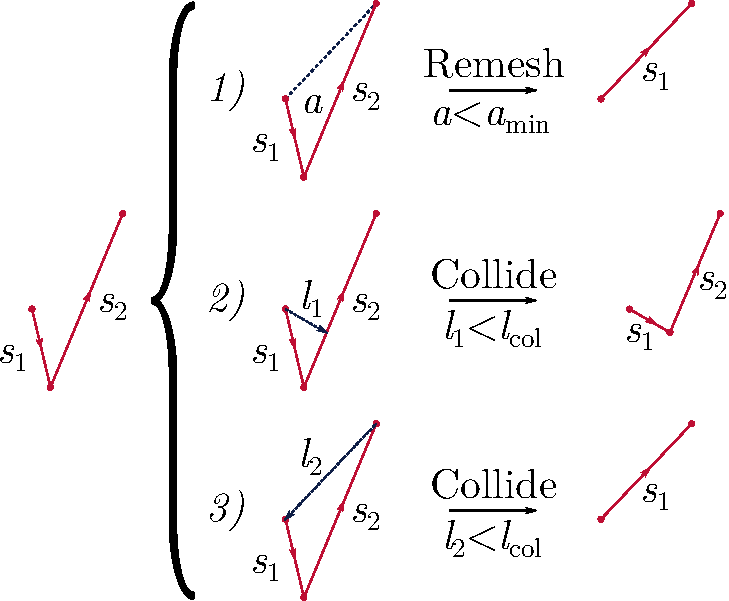
\includegraphics[width=0.7\linewidth]{hinge.pdf}
    \caption[A single dislocation hinge can lead to three different final topologies.]{A single dislocation hinge can lead to three final topologies (two of which are degenerate), the conditions for which can be simultaneously met in any combination. Where $a$ is the enclosed area, $l_1$ and $l_2$ are possible minimum lengths between both segments.}
    \label{f:hinge}
\end{figure}

The combination in which the conditions can be met, and the order in which they are checked could have drastic downstream consequences (see \cref{s:nonCommutativity}). \emph{Especially} at high dislocation densities where multiple collisions happen at every timestep. This had not been an issue prior to many of the improvements made to the codebase, but with the increased ability to model a larger number of dislocations to a sufficiently advanced point where this was having a significant impact, particularly in Haiyang Yu's nanoindentation simulations, which would either go wrong by creating unphysical junctions and/or massively slow down after reaching a certain point.

This was a multi-stage fix, where each fix progressively uncovered more and more shortcomings resulting from the unavoidable coupling between topological operations. These progressive fixes are detailed in \cref{s:nonCommutativity}. Here we will only focus on problems with collisions.

The first fix involved prioritising hinge collisions above the other type of collision, which we call \emph{two-line} collision. This meant detecting and resolving all possible hinge collisions before detecting and resolving any two-line collision. The rationale behind this is that segments in a hinge are already part of a single dislocation line. Because they are connected to each other at a single hinge node, they are already interacting via line tension and remote interaction; whereas two unconnected segments approaching one another only interact via remote interaction. The other, more practical advantage of resolving hinges first is that hinge collisions decrease the total segment length of the involved segments, therefore reducing their collision radii and the probability of them colliding with other segments via two-line collisions.

The second was much more subtle. \Cref{f:hinge} has two options for colliding a hinge, as seen in \cref{f:hinge}. Both resulting in different topologies. Which topology we ended up with was down to which segment, $s_1$ or $s_2$, the code came across first. If $s_1$ was first, then the answer would be $2)$, otherwise it would be $3)$. At the very least, the answer should be the same for a given network topology, regardless of how it is represented. So we decided to ensure the distance calculated was always the minimum out of both scenarios. Which means the distance calculated should be the minumum distance between the non-hinge node of the short segment, to the long segment. There is an argument to be made that the solution should be the other way round, as that would ensure the final structure has the minimum total length, as well as one less node. However, this could potentially leave many hinges around that would have otherwise been resolved.

\subsection{Collision distance}\label{ss:collisionDistance}

In the same vein as \cref{ss:hinges}, two-line collisions were being improperly prioritised. They occurred arbitrarily as the code came across them. Again yielding different answers for different representations of the same network. Only this time it had to do with the collision radius, as shown in \cref{f:collisionRadius}.
\begin{figure}
    \centering
    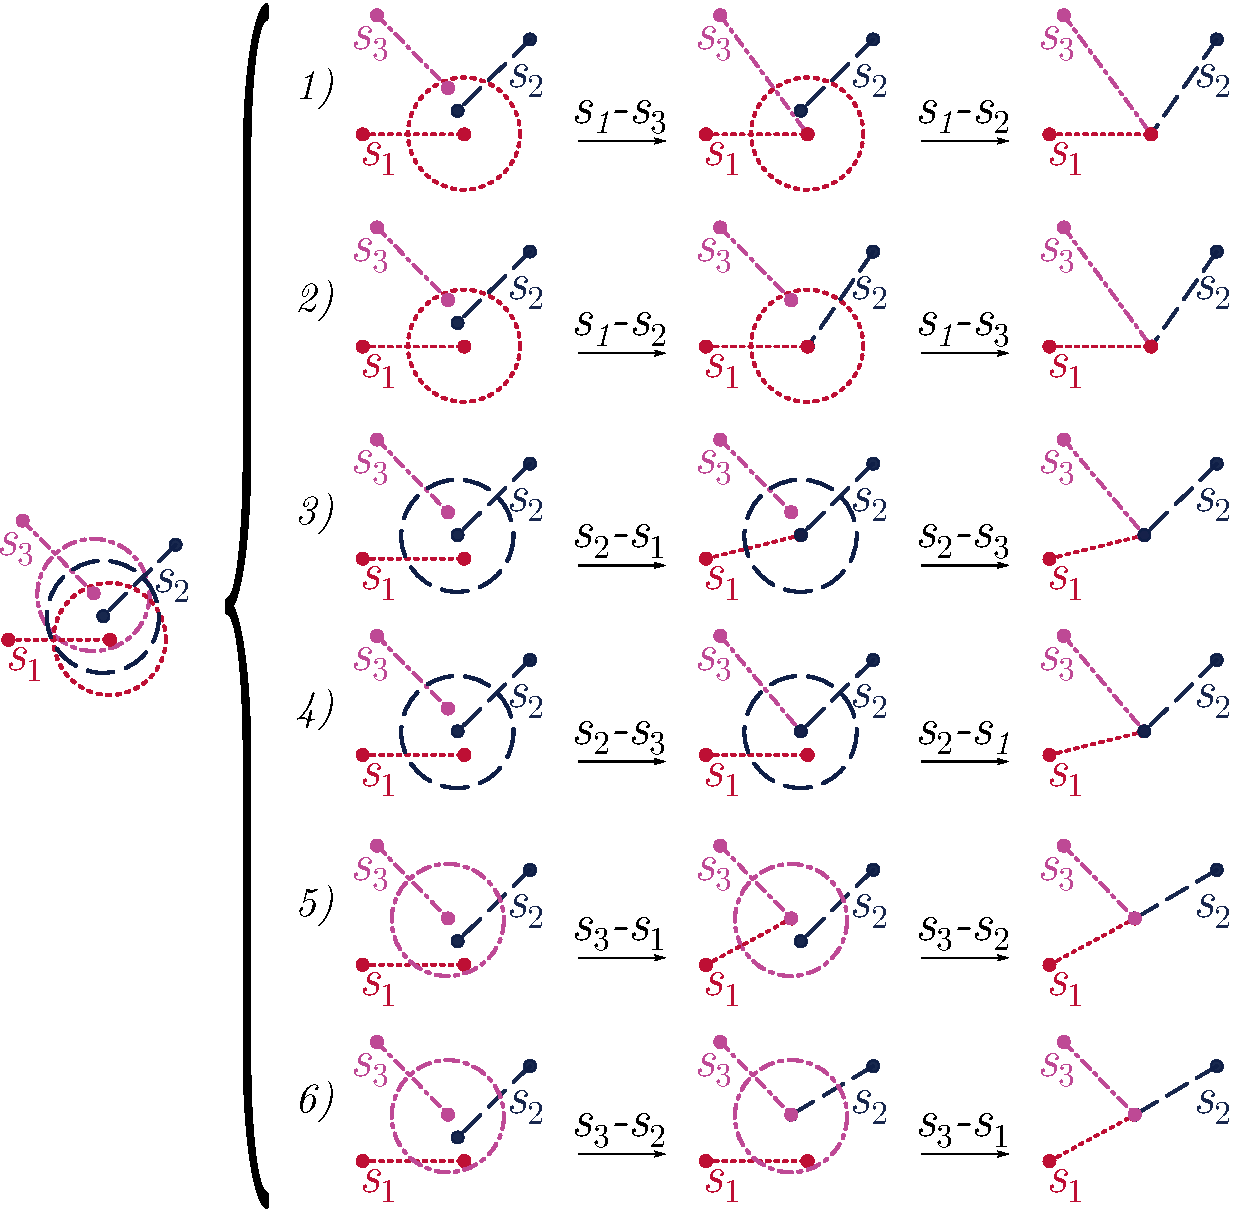
\includegraphics[width=0.9\linewidth]{collisionDist.pdf}
    \caption[Dislocation segments inside different collision radii.]{Multiple dislocation segments inside the same collision radius. Resolving all collisions at once leads to 3 different structures, 6 total but half are degenerate. Circles represent collision radii for the segments with corresponding line style and colour.}
    \label{f:collisionRadius}
\end{figure}

The actual algorithm is more sophisticated because it accounts for whole segments, as well as their relative velocities. It returns the points along the segments that minimise the distance between segments. These points are then used to decide which nodes and how they should be merged.

The problem was that as soon as a viable collision was found, the function returned. So in a scenario like \cref{f:collisionRadius}, if the code was looking for a collision on $s_1$, and it came across $s_3$ first, it would flag that as the collision, disregarding the fact that not only was $s_2$ closer, but $s_2$ and $s_3$ are also closer; and perhaps the true minimal distance was not even between $s_1$ and another segment, but between $s_2$ and $s_3$. We had to apply the same fix to hinge collisions. Admittedly, it matters less in that case as they tend to be rarer, plus their size is limited anyway, but still ensures a more correct solution.

The original algorithm had $\mathcal{O}(N^2)$, $\Theta(N^2/4)$ and $\Omega(N)$ for its upper, average, and lower bounds respectively for fixed $N$, where $N$ is the number of segments. The new one is always $\mathcal{O}(N^2)$. However, $N^2/4 \to N^2$ as $N\to\infty$, so as simulations grow larger, the performance hit gets lower. Moreover, the algorithm is quite cheap compared to other processes, and the improved accuracy is very much worth the small cost.

Better collision detection tends to result in faster simulations because the resulting structures are guaranteed to either produce the shortest segments---which can be cleaned up by remeshing---and therefore more accurate junctions. Referring back to \cref{f:collisionRadius}, it is evident that the structure formed by colliding $s_1$ and $s_3$ is higher energy than that formed by colliding $s_1$ and $s_2$. In this case, if we fully resolve the two possible collisions for every combination of segments, we arrive at three different scenarios (6 total but half are degenerate). However, this still leaves room for producing different answers given different representations of the network. If, for example the most appropriate collision is $s_2$-$s_3$ (cases 4 and 6 in \cref{f:collisionRadius}), the order in which it is performed can yield two slightly different structures after resolving the remaining collisions. However, this is preferrable over finding other, less favourable collisions that may lead to unecessarily complex structures.

We must also bear in mind that \cref{f:collisionRadius} shows a minimal example for a case where three collision radii overlap, and the resulting structures are not dissimilar to one another. In fact, if the final junction formed is glissile, they should evolve similarly. However, as the code was now able to handle and evolve larger numbers of dislocations further than before, it became apparent that the collision algorithms needed to be improved. After all, as the number of candidate collisions increased, so did the chance for the code to pick the wrong one and for that to have a deleterious effect on the code.

\section{Separation}\label{s:separation}

One of the larger problems with high dislocation densities, is the computational complexity of the separation function. Its role is to take high energy, highly connected structures and break them apart into lower energy, lower connection ones. The separation criteria is the power dissipation of the split configuration, compared to the power dissipation of the unseparated structure. The power dissipation is given by
\begin{align}\label{eq:powerDiss}
    W_m & = \sum\limits_i^N\vec{v}_i \cdot \vec{f}_i\,,
\end{align}
where $W_m$ is the power dissipation of splitting mode $m$, $\vec{v}_i$ is nodal velocity, and $\vec{f}_i$ the nodal force of node $i$ participating in the splitting mode. Locality is assumed, so the computation of the pre-separation---reference---power dissipation involves only the node to be separated ($N=1$); whereas the computation of the post-separation power dissipation involves the two nodes the node splits into ($N=2$). The splitting mode chosen by the separation subroutine is that which dissipates the largest amount of power. If the pre-separation node has a higher power dissipation than any separation mode, it remains unseparated. In practice, the reference power dissipation is multiplied by a factor 1.05 to prevent nodes from flickering between being separated and colliding over multiple timesteps until the nodes can move far enough apart that they no longer collide.

Separation is a very poorly scaling operation. For a single multi-connected node we have,
\begin{align}
    M & = \left(\sum\limits_{j=2}^{\left\lfloor C/2 \right\rfloor} \dfrac{C!}{(C-j)! j!}\right)\,.
\end{align}
Where $C$ is the number of connections a node has, $j$ the number of connections in a splitting mode\footnote{This is the number of connections taken by one node after the split, the other would retain $C-j$ connections.}, and $M$ is the total number of splitting modes. Mirror symmetries where $C = 2j$ half the number of possible splitting configurations in those cases. This type of scaling leads to a combinatorial explotion in computational complexity at higher connectivities. At best, this puts the lower bound at approximately Sterling's factorial formula $N! \approx \Omega(N\log{N})$ for large $N$. Furthermore, all of these configurations must be generated---an $\mathcal{O}(M)$ operation, where $M$ are the number of nodes to be added---in order to check their power dissipation. Unfortunately, this is a relatively expensive operation because the code dynamically expands the relevant arrays. The nodal velocities and segment forces must then be calcualted for every configuration. Whichever has the largest energy dissipation---provided it is higher than the reference configuration---is picked as the final configuration. Since locality is assumed, only the forces and mobilities of the nodes and segments directly involved in the split are accounted for, however this still involves an $\mathcal{O}(2 N)$ call to the remote force calculation per splitting mode. Since the procedure must be performed for all nodes exceeding the maximum allowed connectivity, it is extremely important that individual nodal connectivities as well as, the total number of highly connected nodes, remain as low as possible.

The solution may appear to be as simple as calling separation after resolving a single collision. Then looping through all collisions in a given timestep. However, this can cause collisions to be undone, leading to an infinite loop. Solving this was a long, multi-stage process. However, the solution is rather simple and elegant. We simply applied the power dissipation criteria to the collision-separation loop as described by \cref{alg:collisionSep}.
\begin{algorithm}
    \caption{Collision-separation algorithm with power dissipation.}
    \label{alg:collisionSep}
    \begin{enumerate}
        \item Set up \texttt{s1Skip} and \texttt{s2Skip}, which are empty buffers for skipping pairs of corresponding segments in the collision detection.
        \item Detect collision, skips corresponding segment pairs in \texttt{s1Skip} and \texttt{s2Skip}. Among the return values are the colliding segments \texttt{s1} and \texttt{s2}.
        \item If no collision was detected, exit collision-separation loop and carry on with the simulation.
        \item If a collision was detected, resolve collision. Among the return values are the pre-collision power dissipation and the node merged into, \texttt{mergednodeid}.
        \item Separate multiply connected nodes, among the return values is the maximum power dissipation post-separation for node \texttt{mergednodeid}. If node \texttt{mergednodeid} is not separated, this value is zero. Otherwise, it is equal to the maximum power dissipation; be it from the unseparated \texttt{mergednodeid}, or the nodes it separated into.
        \item If the power dissipation post-separation is larger than the power dissipation pre-collision, then clear \texttt{s1Skip} and \texttt{s2Skip}, update the network and auxiliary matrices, and return to 2. Else, add \texttt{s1} and \texttt{s2} to \texttt{s1Skip} and \texttt{s2Skip} respectively, don't update the network and auxiliary matrices, and return to 2.
    \end{enumerate}
\end{algorithm}

This can lead to collisions being checked more than once, but in keeping with the quasi-static assumption, ensures the network is always in a first-order minimum energy configuration.\footnote{A true minimal energy structure would require all collisions to be performed at once, and a full, global traversal of every splitting mode tree.}

It is worth noting that nodes labelled as immobile (an artificial construct to mimic pinning) are not split by separation. Which means they sometimes become very highly connected, and as a result can create an impassable obstacle for other nodes. As a result, they get `unpinned' when they reach a critical level of connectivity. Separation is performed after this check to break them apart, and also because nodes may need separating despite there being no collisions during the timestep.

It is worth noting that the power dissipation criterion has not been used in \cref{c:simulations} as this change was completed some time after the simulations started running. Instead, they use an out-dated method that simply checks whether the pre-collision and post-separation networks have the same number of nodes and segments. If they do, then the network and auxiliary matrices are not updated and the colliding segments get added to \texttt{s1Skip} and \texttt{s2Skip}, otherwise the buffers are emptied and the collision-separation is allowed to happen. This can miss some collisions, so after the collision-separation loop, we collide the rest of the nodes and exit. The outer call to separation deals with these as it sees fit.

This is an imperfect solution as a node may be separated into a different configuration than it was initially. It also can create highly connected nodes, but nowhere near as many or as highly connected as before. However, this was the method available to us at the time and was still a huge improvement over the previous one.

\section{Surface remeshing}
\label{c:surfRem}

Most of the improvements to remeshing subroutines were done by Bruce Bromage, including the surface remeshing. His work on dislocation displacements necessitated the surface and virtual remeshing to be accurate. Among these requirements is the need to prevent dislocations from exiting out of surfaces with fixed displacements. If we take \cref{f:tensileSetupTop}, which describes the displacement boundary conditions for \cref{c:simulations}, we see two surfaces upon which displacements are specified.
\begin{figure}
    \centering
    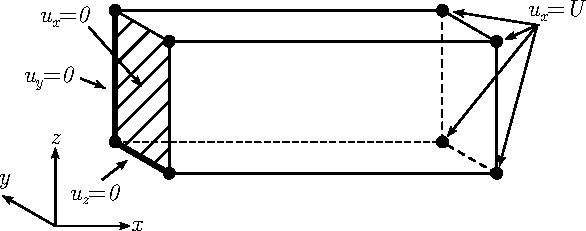
\includegraphics[width=0.8\linewidth]{tensileSetup.pdf}
    \caption[Displacement boundary conditions for dislocation plasticity modelling of single crystal, micro-tensile tests.]{Displacement boundary conditions for dislocation plasticity modelling of single crystal, micro-tensile tests.}
    \label{f:tensileSetupTop}
\end{figure}
Having dislocations exit those surfaces creates a slip step on them. This leads to very high stresses because the FEM essentially has to push the slip step back in order to make it conform to the displacement boundary conditions as in \cref{f:slipStep}. This is unphysical, as in reality the dislocations simply move into the bulk of the material, which is not modelled. In the bulk, they stop experiencing the Peach-K\"{o}hler force, because it is not subject to the forces or displacements of the experiment, so they pile up as the only forces they experience are those from themselves and other dislocations.
\begin{figure}
    \centering
    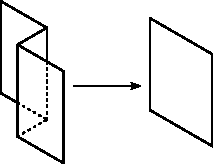
\includegraphics[width=0.5\linewidth]{slipStep.pdf}
    \caption{Slip step created by a dislocation exiting the volume has to be moved back to enforce displacement boundary conditions.}
    \label{f:slipStep}
\end{figure}

This was originally hard-coded for cantilever bending, but a general solution can be found with \cref{eq:signedDist},
\begin{align}\label{eq:signedDist}
    D & = \hat{\vec{n}} \cdot (\vec{x_0} - \vec{x_n})\,,
\end{align}
where $D$ is the signed distance from the point, $\vec{x_0}$, to a plane with unit normal, $\hat{\vec{n}}$, which passes through the point, $\vec{x_n}$. $D$ is positive if point $\vec{x_0}$ is on the side $\hat{\vec{n}}$ points towards and negative otherwise. We can identify nodes that have exited from these surfaces by using their surface normal, a point on them, and whether $D$ is positive. They can then be moved back to the surface and pinned.

This is an imperfect solution, but works quite well and removes these nodes from the mobility calculation. Perhaps a better solution would be to flag those nodes such that Peach-K\"{o}ler forces, tractions, displacements, and surface remeshing criteria no longer apply to them. However, this will have to be implemented and tested as part of future improvements to the code.

\section{Conclusions}

Discrete dislocation dynamics is a stiff and chaotic dynamical system. It is very sensitive to small changes, as we will see in \cref{c:tractions}. Having a correct topology is of the utmost importance in this regard. Something as small as a collision that was not performed when it should have, can have dramatic downstream consequences. As dislocation density increases, the degree of correctness when resolving their interactions increases in importance. Not only does it increase the accuracy of a simulation, but improves its running speed.

The increase in accuracy is obvious; detecting all the collsions that should be detected; resolving them in a manner more keeping with the quasi-static assumption yielding the mobility law; and ensuring the network resolution is what it should be; make for more accurate simulations.

Part of the increase in running speed is down to the fact that quasi-static conditions are better met than before, so the timsetep can be greater. The other huge benefit to running speed is down to the asymptotic scaling and high scaling constants of the algorithms we use; $\mathcal{O}(N^2)$ for seg-seg forces and collisions; $\mathcal{O}(C!)$ for a single separation; $\mathcal{O}(M N)$ for tractions. Where $N$ is the number of segments, $C$ the number of connections, and $M$ the number of surface elements. Simply put, we disproportionately benefit from having fewer items these expensive functions operate over.

With these improvements, simulations that used to be computationally intractible within a reasonable timeframe are now very doable. Large, complex simulations with high dislocation densities are still slow by virtue of how topologically active they can be and due to the high cost of the remote forces, but they are simultaneously more accurate and faster by multiple orders of magnitude (sometimes 5 or more) than before.
\savearabiccounter
%3485 words
\chapter{Dislocation-induced surface tractions}
\label{c:tractions}

\Cref{s:numericVsAnalytic} have been adapted from a manuscript prepared for publication. \Cref{s:parallel} outlines the work done in parallelising the analytic traction calculation on GPUs.

\section{Numeric v.s. analytic tractions}\label{s:numericVsAnalytic}

\subsection{Introduction}\label{ss:paperIntro}

Simulations are essential for interpreting experimental data and relating the measured mechanical response to dislocation mechanisms \cite{0965-0393-6-6-007,doi:10.1080/14786430500341250,tarleton2015discrete,YU2018}. Experimentally, we are limited by the electron transparency of the material and our capacity for subjecting samples to representative loads whilst simultaneously keeping dislocations in focus. Modelling, albeit imperfect and idealised, can greatly inform our understanding and provide insight into the dislocation dynamics responsible for our observations.

Simulating micromechanical tests with explicit dislocation interactions necessitates the coupling of discrete dislocation dynamics (DDD) to the finite element method (FEM) \cite{Groh2009}. One of the simples and most popular ways of doing so is the superposition method \cite{superposition_scheme0,superposition_scheme1,superposition_scheme2}. Which works by decomposing the problem into separate DDD and FE problems as illustrated by \cref{f:superposition_scheme}.
\begin{figure}
    \centering
    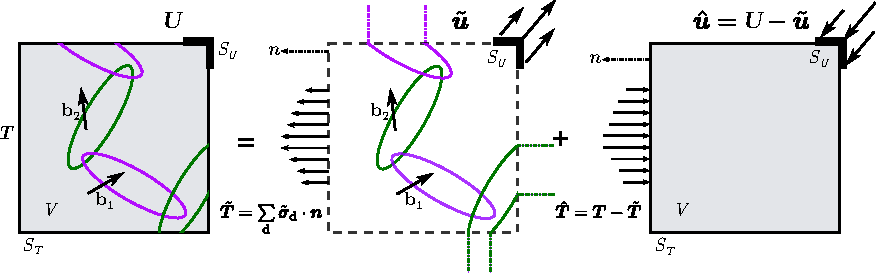
\includegraphics[width=\linewidth]{fem_ddd.pdf}
    \caption[Superposition Model for DDD-FEM coupling.]{The superposition used to couple DDD and FEM. The volume $V$ is bounded by a surface $S = S_{T} \cup S_{U}$ and contains a dislocation ensemble and is subjected to tractions $\vec{T}$ on $S_{T}$ and $\vec{U}$ on $S_{u}$. First, the traction, $\vec{\tilde{T}}$, and displacement, $\vec{\tilde{u}}$, fields due to the dislocations in the infinite domain (DDD) are evaluated on the boundaries $S_{T}$ and $S_{U}$ respectively. Then an elastic boundary value problem can be solved with FEM to calculate the corrective elastic fields required to satisfy the boundary conditions $\vec{\hat{T}} = \vec{T} - \vec{\tilde{T}}$ and $\vec{\hat{u}} = \vec{U} - \vec{\tilde{u}}$.}
    \label{f:superposition_scheme}
\end{figure}

Specifically, a linear-elastic solid $V$ bounded by a surface $S$ is subjected to traction boundary conditions, $\vec{T}$, on $S_{T}$ and displacement boundary conditions, $\vec{U}$, on $S_{U}$. The ($\tilde{~}$) fields are those generated by the dislocations in an infinite solid and in our case are obtained by evaluating analytic solutions in a DDD simulation \cite{a_non-singular_continuum_theory_of_dislocations}. Formally, the dislocation field satisfies,
\begin{align}
     & \left.
    \begin{array}{l}
        \nabla \cdot \tns{\tilde{\sigma}} = \bm{0}                 \\
        \tns{\tilde{\sigma}} = \tns{C} : \tns{\tilde{\varepsilon}} \\
        \tns{\tilde{\varepsilon}} = \frac{1}{2} \left( \nabla \vec{\tilde{u}} + (\nabla \vec{\tilde{u}})^T \right)
    \end{array}
    \right\} \quad \textrm{in V}                                                   \\
    %
     & \tilde{\tns{\sigma}} \cdot \vec{n} = \tilde{\vec{T}} \quad \textrm{on } S_T \\
    %
     & \left.
    \begin{array}{l}
        \vec{\tilde{u}} = \vec{\tilde{U}}, \quad t>0 \\
        \vec{\tilde{u}} = \bm{0}, \quad t=0
        \label{eq:utildebc}
    \end{array}
    \right\} \quad \textrm{on } S_U \,.
\end{align}
%
As the dislocation fields do not vanish on $S$, the dislocations load the volume by generating tractions, $\tilde{\vec{T}}$, on $S_T$ and displacements, $\vec{\tilde{u}}$, on $S_U$. This additional loading deforms $V$, generating an additional ``image'' stress which the dislocations then feel. Therefore, corrective ($\hat{~}$) fields must be superimposed to satisfy the desired boundary conditions. The corrective field which accounts for both the applied and image stress is obtained numerically by solving the elastic boundary value problem,
%
\begin{align}
     & \left.
    \begin{array}{l}
        \nabla \cdot \tns{\hat{\sigma}} = \bm{0}               \\
        \tns{\hat{\sigma}} = \tns{C} : \tns{\hat{\varepsilon}} \\
        \tns{\hat{\varepsilon}} = \frac{1}{2} \left( \nabla \vec{\hat{u}} + (\nabla \vec{\hat{u}})^{T} \right)
    \end{array}\right\} \quad \textrm{in V}                                                  \\
    %
     & \hat{\tns{\sigma}}\cdot\vec{n} = \vec{T} - \tilde{\vec{T}} \quad \textrm{on } S_T \label{eq:thatbc} \\
    %
     & \vec{\hat{u}} = \vec{U} - \vec{\tilde{U}} \quad \textrm{on } S_U \,. \label{eq:uhatbc}
\end{align}
%
Once the solutions to both problems are known, their superposition solves the desired mixed boundary value problem,
%
\begin{align}
     & \left.
    \begin{array}{l}
        \nabla \cdot \tns{\sigma} = \nabla \cdot \left( \tns{\hat{\sigma}} + \tns{\tilde{\sigma}} \right) = \bm{0}                                                              \\
        \tns{\sigma} = \tns{\hat{\sigma}} + \tns{\tilde{\sigma}} = \tns{C} : \left( \tns{\hat{\varepsilon}} + \tns{\tilde{\varepsilon}} \right) = \tns{C} : {\tns{\varepsilon}} \\
        \tns{\varepsilon} = \tns{\hat{\varepsilon}} + \tns{\tilde{\varepsilon}} = \frac{1}{2} \left( \nabla ( \vec{\hat{u}} + \vec{\tilde{u}} ) + \left[ \nabla ( \vec{\hat{u}} + \vec{\tilde{u}} ) \right]^T \right) = \frac{1}{2} \left( \nabla \vec{u} + ( \nabla \vec{u} )^{T} \right)
    \end{array}
    \right\}\quad \textrm{in V}                                    \\
    %
     & \tns{\sigma} \cdot \vec{n} = \vec{T} \quad \textrm{on } S_T \\
    %
     & \left.
    \begin{array}{l}
        \vec{u} = \vec{U}, \quad t>0 \\
        \vec{u} = \bm{0}, \quad t=0
    \end{array}
    \right\} \quad \textrm{on } S_U\,.
    \label{eq:ubc}
\end{align}

For all its simplicity and elegance, the method is not without issue. As the distance between dislocation and surface decreases, $\tns{\tilde{\sigma}}$ diverges \cite{boundary_problems_in_dd}. This can be partially solved by using a non-singular formulation for $\tns{\tilde{\sigma}}$, such as that proposed by \citet{a_non-singular_continuum_theory_of_dislocations}. Regardless, the steep gradients in the dislocation field are difficult to accurately capture as the dislocation approaches $S$. Another problem with this method is the large computational cost when simulating a heterogeneous solid, as this requires calculating polarisation stresses due to the difference in the elastic constants between phases \cite{superposition_scheme0,boundary_problems_in_dd,ddd_precipitate}.

A modified superposition scheme \cite{ODay2004} can overcome this by dividing the problem into separate DDD-FEM problems coupled through an elastic FE problem. This requires accurate evaluation of $\vec{\tilde{T}}$ on the domain boundaries---which can only be captured with a fine FE mesh---increasing the computational cost. Therefore, simulating polycrystalline or composite materials using superposition necesitates methods to accurately evaluate both $\vec{\tilde{u}}$ and $\vec{\tilde{T}}$. The displacements can be evaluated analytically as shown by \cite{bromage2018calculating} and this paper investigates the evaluation of the dislocation tractions analytically.

As previously mentioned, the relative simplicity of the superposition method has made it a popular choice for coupling DDD and FEM as all it needs is the evaluation of FE nodal forces and displacements on the boundary. Furthermore, the analytic expression for the stress field produced by a finite, straight dislocation line segment has allowed \citet{analytic_tractions} to use the non-singular formulation \cite{a_non-singular_continuum_theory_of_dislocations} to obtain closed-form solutions for the tractions generated by the segment on the surface of a finite element.

\subsection{Theory}\label{ss:paperTheory}

The force exerted by a dislocation ensemble on a node, $a$, belonging to element, $e$, is given by,
%
\begin{align}
    \vec{F}_{a} = \int_{S_{e}} \left[\tns{\tilde{\sigma}}(\vec{x}) \cdot \vec{n}\right] N_{a}(\vec{x})\; \mathrm{d}S_{e}\,.
    \label{eq:ddd_fem_force}
\end{align}
%
Where $\mathrm{d}S_{e}$ is the surface of element $e$ with surface area $S_{e}$, and $N_{a}$ is the finite element shape function for node $a$. The solutions are for linear rectangular surface elements and as such the shape functions are,
\begin{align}
    \label{eq:shape_function}
    N_{1} & = \dfrac{1}{4}(1-s_1)(1-s_2)             \\
    N_{2} & = \dfrac{1}{4}(1+s_1)(1-s_2)\nonumber    \\
    N_{3} & = \dfrac{1}{4}(1+s_1)(1+s_2)\nonumber    \\
    N_{4} & = \dfrac{1}{4}(1-s_1)(1+s_2)\nonumber\,.
\end{align}
Where $s_1$ and $s_2$ are the orthogonal coordinates local to the element.

Gauss quadrature is usually used to numerically evaluate the surface integral in \cref{eq:ddd_fem_force}. In 1D this is,
%
\begin{align}
    \label{eq:gauss_leg}
    \int\limits_{-1}^{1} f(s)\;\mathrm{d}s \approx \sum\limits_{i=1}^{n} w_{i} f(s_{i}) \quad \textrm{where}\quad
    %
    w_{i} = \dfrac{2}{\left(1-s_{i}^{2}\right) \left[P_{n}^{'}\left(s_{i}\right)\right]^{2}}\,,
\end{align}
%
is the weighting of the Gauss point, $s_{i}$, which is the $i\textsuperscript{th}$ root of the $n\textsuperscript{th}$ normalised Legendre polynomial, $P_{n}(1) = 1$. $P_{n}^{'}$ is the first order derivative of $P_{n}$. This method is very accurate for functions that can be accurately approximated by polynomials. In fact, for a polynomial of degree $n$, one needs $n-1$ points to obtain an exact numerical solution. However, this quadrature is well-known for being unsuitable for integrating functions with poles or near-poles \cite{gauss_leg, gauss_leg_sing}.

We avoid the strict pole in $\tns{\tilde{\sigma}}$ by using the non-singular formulation described in \cite{a_non-singular_continuum_theory_of_dislocations}, where the true singularity is avoided by adding a small cut-off radius to account for the dislocation core. However, if an integration point falls close to, or within the dislocation core, Gauss quadrature can still produce large errors.

For rectangular surface elements, we must transform from the parent element in $(s_1,\,s_2)$ in \cref{eq:gauss_leg} to the real element coordinate system $(x\,,y\,,z)$. Evaluating \cref{eq:ddd_fem_force} in the parent element and mapping to the real element gives the force on node $a$,
\begin{align}
    \label{eq:gauss_leg_ddd_fem_force}
    \vec{F}_{a} \approx \sum\limits_{i=1}^{Q} w_{i} \sum\limits_{j=1}^{Q} w_{j} [\tns{\tilde{\sigma}}(r_{i}, s_{j})\cdot \vec{n}] N_{a}(r_{i}, s_{j}) \det(\mtx{J})\,.
\end{align}
Where the sum is over the $Q$ quadrature points and $J_{ij} = dx_{i}/ds_{j}$, is the element Jacobian defining the transformation from $(s_1,\,s_2) \mapsto (x,\,y)$. Since the real element is rectangular with surface area $S_e$, then $\det(\mtx{J}) = S_e/4$. \Cref{f:2d_gaussian_quad} contains examples of how the Gauss points are distributed on the surface.
\begin{figure}
    \centering
    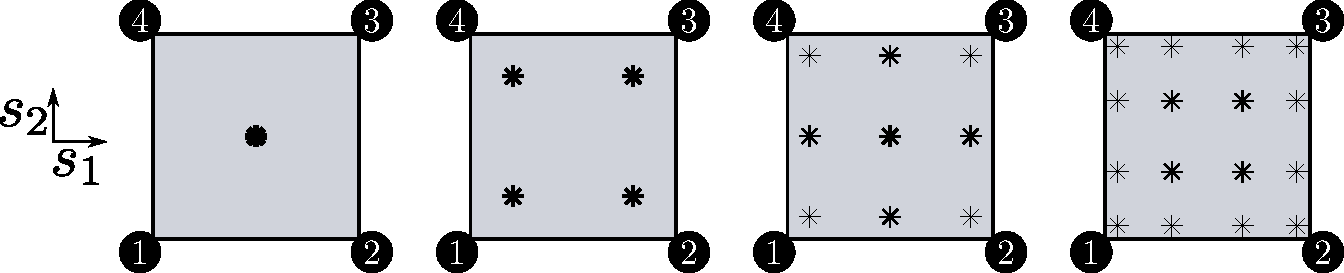
\includegraphics[width=\linewidth]{2d_gaussian_quad.pdf}
    \caption[2D Gauss-Legendre quadrature on quadrangles.]{Examples of 2D Gauss-Legendre quadrature of the parent element with $Q = 1,\, 2,\, 3,\, 4$. The point size represents the weight $w$ of the integration point. The parent elements are centred at the origin and $s_1,\, s_2 \in [-1,\,1]$. We use an anticlockwise node numbering scheme.}
    \label{f:2d_gaussian_quad}
\end{figure}

\begin{figure}
    \centering
    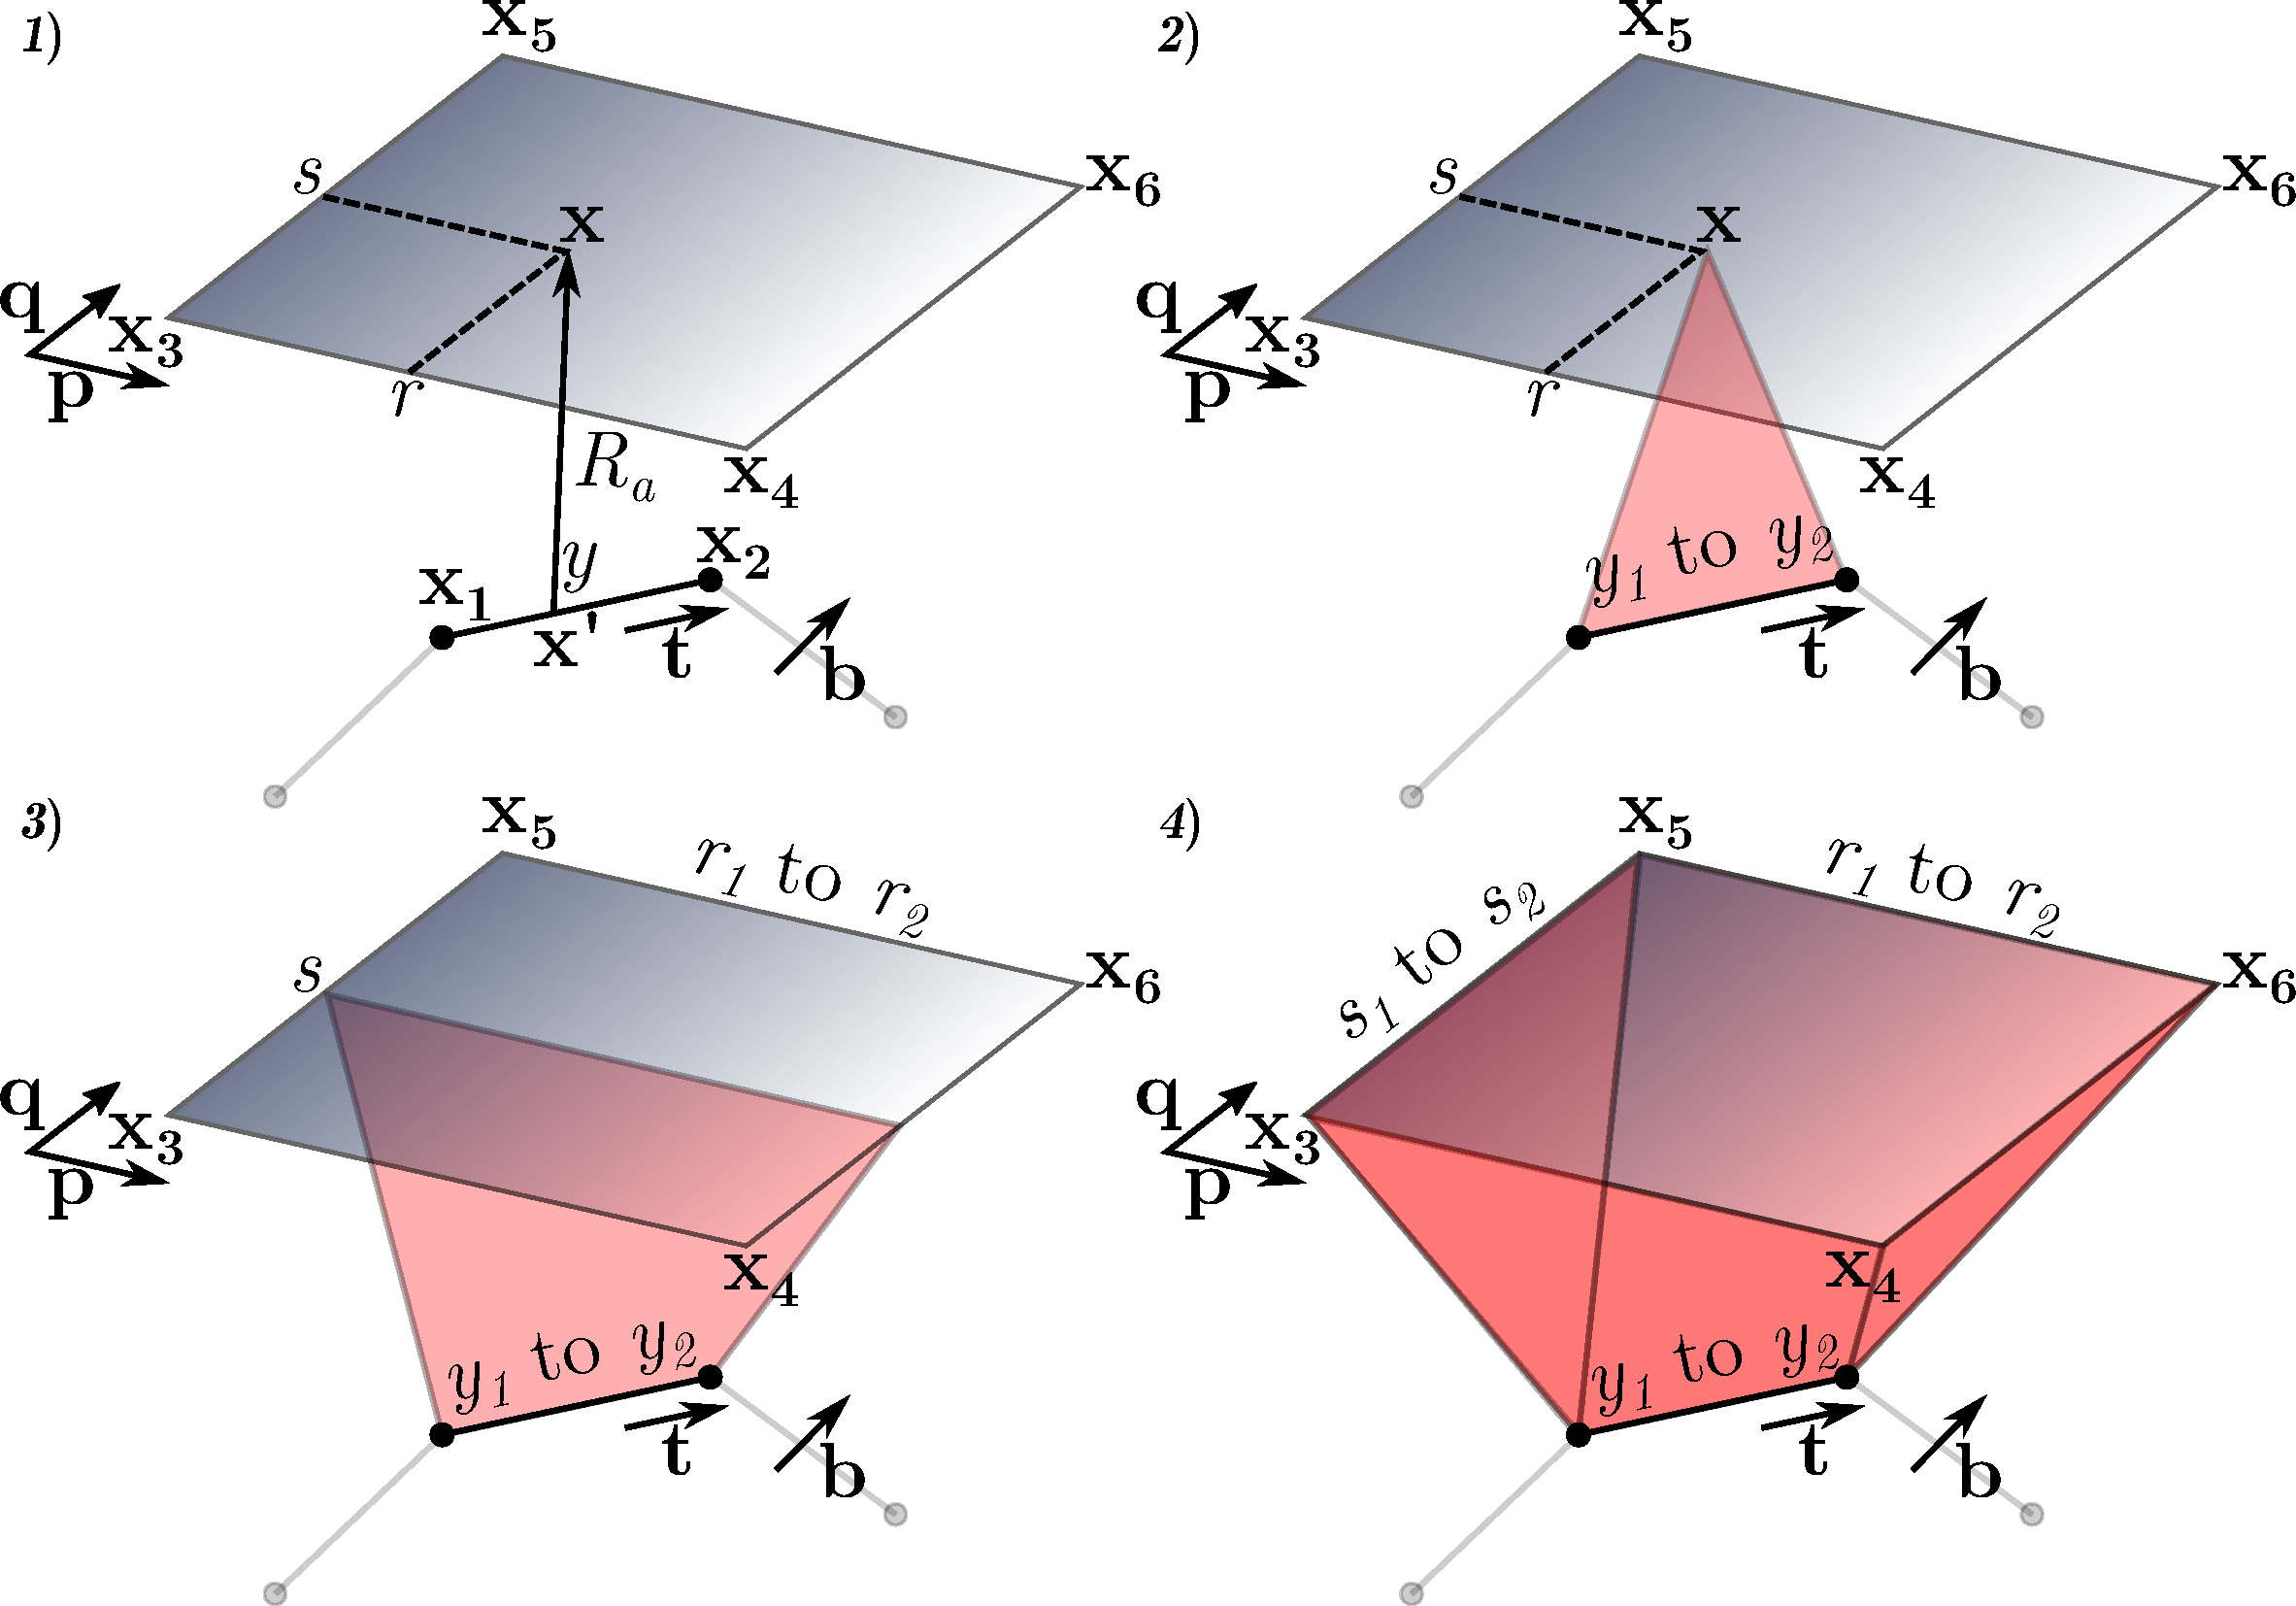
\includegraphics[width=0.8\linewidth]{force_calc_linear_rectangle.pdf}
    \caption[Analytic tractions on linear rectangular surface elements.]{Diagram of the parametric line integrals solved by \citet{analytic_tractions} to find the forces on linear rectangular surface elements.}
    \label{f:force_lin_rect}
\end{figure}
Explicitly, \cref{eq:ddd_fem_force} is actually a triple vector integral as shown in \cref{f:force_lin_rect}. This is because given the isotropic Burgers vector distribution proposed in \cite{a_non-singular_continuum_theory_of_dislocations}, the dyadic form of the stress tensor produced by a straight, finite dislocation segment bounded by nodes at $\vec{x_1}$ and $\vec{x_2}$ \cite{analytic_tractions} is,
\begin{align}
    \label{eq:stress}
    \tns{\tilde{\sigma}}(\vec{x}) = &
    - \dfrac{\mu}{8\pi} \int\limits_{\vec{x_1}}^{\vec{x_2}} \left( \dfrac{2}{R_{a}^{3}} + \dfrac{3a^2}{R_{a}^{5}} \right) \left[ \left(\vec{R} \times \vec{b}\right) \otimes \mathrm{d}\vec{x'} + \mathrm{d}\vec{x'} \otimes \left(\vec{R} \times \vec{b}\right) \right]          \\
    %
                                    & + \dfrac{\mu}{4\pi(1-\nu)} \int\limits_{\vec{x_1}}^{\vec{x_2}} \left( \dfrac{1}{R_{a}^{3}} + \dfrac{3a^2}{R_{a}^{5}} \right) \left[ \left(\vec{R} \times \vec{b}\right) \cdot \mathrm{d}\vec{x'} \right]\vec{I_2}\nonumber                  \\
    %
                                    & -\dfrac{\mu}{4\pi(1-\nu)} \int\limits_{\vec{x_1}}^{\vec{x_2}}  \dfrac{1}{R_{a}^{3}} \left[ \left(\vec{b} \times \mathrm{d}\vec{x'}\right) \otimes \vec{R} + \vec{R} \otimes \left(\vec{b} \times \mathrm{d}\vec{x'}\right) \right]\nonumber \\
    %
                                    & + \dfrac{\mu}{4\pi(1-\nu)} \int\limits_{\vec{x_1}}^{\vec{x_2}} \dfrac{3}{R_{a}^{5}} \left[ \left(\vec{R} \times \vec{b}\right) \cdot \mathrm{d}\vec{x'} \right]\vec{R}\otimes\vec{R}\nonumber,
\end{align}
where,
\begin{align}
    \vec{R}            & = \vec{x} - \vec{x'} = y \vec{l} + r \vec{p} + s \vec{q} \\
    %
    R_a                & = \sqrt{\vec{R} \cdot \vec{R} + a^2}                     \\
    %
    \mathrm{d}\vec{x'} & = -\mathrm{d} y \vec{l}\,.
\end{align}
The vectors $\vec{p}$ and $\vec{q}$ are aligned with the edges of the rectangular finite element, $\vec{n} = \vec{p} \times \vec{q}$ is the element surface normal (pointing away from the dislocation), and $\vec{l}$ is parallel to the dislocation line segment as shown in \cref{f:force_lin_rect}. Then (provided $\vec{l}$ is not parallel to $\vec{p}$ or $\vec{q}$) $\vec{R}$ can be expressed in terms of $(\vec{l},~\vec{p},~\vec{q})$ with coefficients,
\begin{align}
    y = \dfrac{\vec{R}\cdot \vec{n}}{\vec{l}\cdot \vec{n}} \label{eq:problem},\quad
    %
    r = \dfrac{\vec{R}\cdot (\vec{q} \times \vec{l})}{\vec{p}\cdot (\vec{q} \times \vec{l})}, \quad
    %
    s = \dfrac{\vec{R}\cdot (\vec{p} \times \vec{l})}{\vec{q}\cdot (\vec{p} \times \vec{l})}\,.
\end{align}

Substituting \cref{eq:stress} and \cref{eq:shape_function} into \cref{eq:ddd_fem_force} yields four long and messy equations (one for each FE node) that were elegantly solved by \citet{analytic_tractions} by utilising the fact that the triple integrals all had the form,
\begin{align}
    H_{ijkl}        & = \int\limits_{r_{1}}^{r_{2}}\int\limits_{s_{1}}^{s_{2}}\int\limits_{y_{1}}^{y_{2}} \dfrac{r^i s^j y^k}{R_{a}^{m}}\label{eq:triple_int} \\
    \textrm{when }m & = 5 \textrm{ then } i,\, j \in [0,\,3],~k \in [0,\,2]\nonumber                                                                          \\
    \textrm{when }m & = 3 \textrm{ then } i,\, j \in [0,\,2],~k \in [0,\,1]\nonumber                                                                          \\
    \textrm{when }m & = 1 \textrm{ then } i = j = k = 0\,.
\end{align}
Using partial differentiation and integration by parts, they found a series of recurrence relations that lead to double and single integrals of similar form to \cref{eq:triple_int}. All of which are used to construct a full, exact solution. The recurrence relations stop working when $i = j = k = 0 \textrm{ and } m = 1,\, 3$. At which point, direct integration of the remaining single and double integrals (the last triple integrals all cancel out in the global calculation) yields six seed functions that are used as the starting point for the recurrence relations. Three of them are logarithms and three either arctangents or---if a discriminant is negative---hyperbolic arctangents. The details of the procedure can be found in \cite{analytic_tractions}.

Although exact, the use of arctangents, hyperbolic arctangents and logarithmic functions, compounded by the large number of recurrence relations is prime territory for error propagation and numerical problems (see \cref{ss:paperMethod}). The problem is particularly egregious when using general purpose compilers instead of high-performance or scientific computing compilers where mathematical functions are implemented more precisely. Such issues must be taken into account when using analytic tractions, which can be done by using numerical tolerances as described in \cref{ss:paperMethod}.

In simulations, tractions are manifested as image stresses calculated by the FE solver at FE nodes. In order to validate and compare the practical differences between analytic and numeric methods, we compare the resulting image stresses from both methods, to the analytic expressions for infinite dislocations in inhomogenous media for edge \cite{head1953edge}, and screw dislocations \cite[p.~59,~64]{hirth1983theory}. We keep the same nomenclature and coordinate system as both infinite-domain solutions. Where the traction surface is the line $x=0$, the dislocation line direction is the positive $z$-direction (pointing out of the page), the dislocation coordinates are represented by $(a,~c)$, and points in the $xy$-plane described by their $(x,\,y)$ coordinates.

The original paper by \citet{head1953edge} has a few typos that have been replicated in other sources. We therefore include the complete and correct expressions in \cref{eq:imageStressAnalyticEdge1,eq:imageStressAnalyticEdge2,eq:imageStressAnalyticScrew}. \citet{head1953edge} gives two basic cases, as described by \cref{f:head_cases}.
\begin{figure}
    \centering
    \begin{subfigure}[b]{0.45\linewidth}
        \centering
        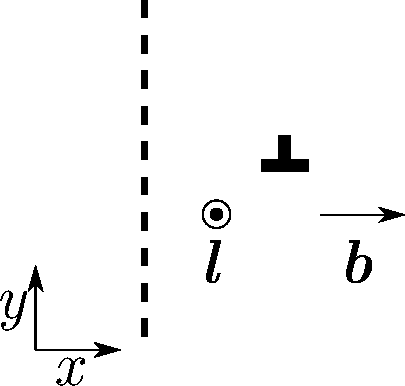
\includegraphics[width=\linewidth]{head_edge_perp.pdf}
        \caption{Edge dislocation with $\vec{b}$ perpendicular to the surface and pointing in the positive $x$-direction ($b \coloneqq \lVert \vec{b} \rVert > 0$).}
        \label{sf:headCase1}
    \end{subfigure}
    ~
    \begin{subfigure}[b]{0.45\linewidth}
        \centering
        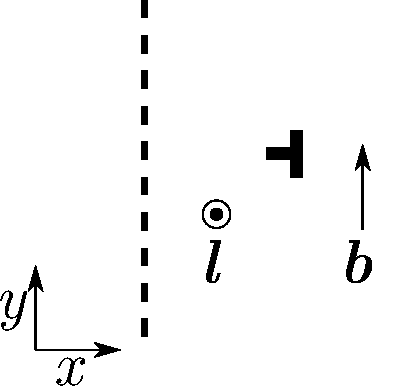
\includegraphics[width=\linewidth]{head_edge_par.pdf}
        \caption{Edge dislocation with $\vec{b}$ parallel to the surface and pointing in the positive $y$-direction ($b \coloneqq \lVert \vec{b} \rVert > 0$).}
        \label{sf:headCase2}
    \end{subfigure}
    \caption{Two cases described by \citet{head1953edge}. In both cases, the line direction points towards the observer and the dashed line is the infinite traction-free boundary.}
    \label{f:head_cases}
\end{figure}
\Cref{eq:imageStressAnalyticEdge1} corresponds to \cref{sf:headCase1}, where $\vec{b}$ is perpendicular to the surface and positive $b$ means it's pointing in the positive $x$-direction,
\begin{subequations}\label{eq:imageStressAnalyticEdge1}
    \begin{align}
        \sigma_{xx} = D (y - c) & \left\{-\dfrac{3 (x - a)^2 + (y - c)^2}{[(x - a)^2 + (y - c)^2]^2} + \dfrac{3 (x + a)^2 + (y - c)^2}{[(x + a)^2 + (y - c)^2]^2}\right.                                             \\\nonumber
                                & \left. + 4 a x \dfrac{3 (x + a)^2 - (y - c)^2}{[(x + a)^2 + (y - c)^2]^3}\right\}\,,                                                                                               \\
        \sigma_{yy} = D (y - c) & \left\{\dfrac{(x - a)^2 - (y - c)^2}{[(x - a)^2 + (y - c)^2]^2} - \dfrac{(x + a)^2 - (y - c)^2}{[(x + a)^2 + (y - c)^2]^2}                                                 \right. \\\nonumber
                                & \left. + 4 a (2 a - x) \dfrac{(x + a)^2 + (3 x + 2 a) (y - c)^2}{[(x + a)^2 + (y - c)^2]^3}\right\}\,,                                                                             \\
        \sigma_{xy} = D         & \left\{(x - a) \dfrac{(x - a)^2 - (y - c)^2}{[(x - a)^2 + (y - c)^2]^2} - (x + a) \dfrac{(x + a)^2 - (y - c)^2}{[(x + a)^2 + (y - c)^2]^2}\right.                                  \\\nonumber
                                & \left. + 2 a \dfrac{6 x (x + a) (y - c)^2 - (x - a) (x + a)^3 - (y - c)^4}{[(x + a)^2 + (y - c)^2]^3}\right\}\,.
    \end{align}
\end{subequations}
\Cref{eq:imageStressAnalyticEdge2} corresponds to \cref{sf:headCase2}, where $\vec{b}$ lies parallel to the surface and positive $b$ means it points in the positive $y$-direction,
\begin{subequations}\label{eq:imageStressAnalyticEdge2}
    \begin{align}
        \sigma_{xx} = D         & \left\{ (x - a) \dfrac{(x - a)^2 - (y - c)^2}{[(x - a)^2 + (y - c)^2]^2} -(x + a) \dfrac{(x + a)^2 - (y - c)^2}{[(x + a)^2 + (y - c)^2]^2} \right.     \\\nonumber
                                & \left. + 2 a \dfrac{(3 x + a) (x + a)^3 - 6 x (x + a) (y - c)^2 - (y - c)^4}{[(x + a)^2 + (y - c)^2]^3}\right\}\,,                                     \\
        \sigma_{yy} = D         & \left\{ (x - a) \dfrac{(x - a)^2 + 3 (y - c)^2}{[(x - a)^2 + (y - c)^2]^2} - (x + a) \dfrac{(x + a)^2 + 3 (y - c)^2}{[(x + a)^2 + (y - c)^2]^2}\right. \\\nonumber
                                & \left. - 2 a \dfrac{(x - a) (x + a)^3 - 6 x (x + a) (y - c)^2 + (y - c)^4}{[(x + a)^2 + (y - c)^2]^3}\right\}\,,                                       \\
        \sigma_{xy} = D (y - c) & \left\{\dfrac{(x - a)^2 - (y - c)^2}{[(x - a)^2 + (y - c)^2]^2} - \dfrac{(x + a)^2 - (y - c)^2}{[(x + a)^2 + (y - c)^2]^2} \right.                     \\\nonumber
                                & \left. + 4 a x \dfrac{3 (x + a)^2 - (y - c)^2}{[(x + a)^2 + (y - c)^2]^3}\right\}\,.
    \end{align}
\end{subequations}
\Cref{eq:imageStressAnalyticScrew} corresponds to screw dislocations, which are markedly simpler as only the shear components are non-zero. Here $\vec{b} = \vec{l}$ so positive $b$ means it points in the positive $z$-direction,
\begin{subequations}\label{eq:imageStressAnalyticScrew}
    \begin{align}
        \sigma_{xz} & = -D \left(\dfrac{y - c}{(x - a)^2 + (y - c)^2} - \dfrac{y - c}{(x + a)^2 + (y - c)^2}\right)   \\
        \sigma_{yz} & = D \left(\dfrac{x - a}{(x - a)^2 + (y - c)^2} - \dfrac{x + a}{(x + a)^2 + (y - c)^2}\right)\,.
    \end{align}
\end{subequations}
In every case, the constant $D$ is defined by \cref{eq:Dconstant},
\begin{align}\label{eq:Dconstant}
    D = \dfrac{\mu}{2\pi} \cdot \dfrac{1+\nu}{1-\nu^2} \cdot b\,.
\end{align}
Note the first terms of \cref{eq:imageStressAnalyticEdge1,eq:imageStressAnalyticEdge2,eq:imageStressAnalyticScrew} all correspond to the stress field generated by the dislocation itself. The following terms are the corrective terms required to make the boundary conditions on the surface equal to zero. Therefore, we can split these equations and only look at the real or corrective terms independently, which we do in order to only visualise the effect of the different traction calculations. Furthermore, \cref{eq:imageStressAnalyticEdge1,eq:imageStressAnalyticEdge2,eq:imageStressAnalyticScrew} are all singular at the dislocation coordinates. Our simulation code uses the non-singular expressions found by \citet{a_non-singular_continuum_theory_of_dislocations}, which smooth out drastic increases in stresses and avoid numerical blow up as we near the dislocation core.

\subsection{Methodology}\label{ss:paperMethod}

Numerical integration of tractions can produces unexpected behaviour such as force hot spots and sign inversions as a dislocation approaches a surface. During a large simulation, these effects are hard to spot.

\citet{analytic_tractions} identified that for a given number of quadrature points, the error is dependent on the dislocation character but always increases rapidly as the distance between the segment and element surface decrease (see \cref{f:rel_err_perp_edge,f:rel_err_par_edge}).

Expanding the test cases reveals just how problematic numerical integration of the tractions can be when a dislocation approaches a surface. The two basic test cases, an orthogonal and parallel edge segment, are shown in \cref{f:gauss_quad_test}.
\begin{figure}
    \centering
    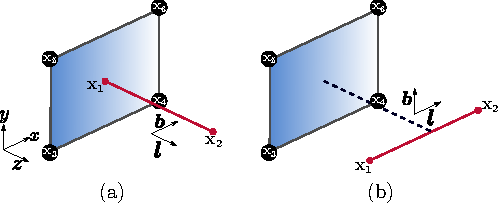
\includegraphics[width=0.8\linewidth]{test_gauss_quad.pdf}
    \caption[Test cases for comparing numeric v.s. analytic tractions using an edge dislocation near a surface.]{Simple test cases for an edge segment and surface element perpendicular (a) and parallel (b). The perpendicular dislocation is centered at the midpoint of the surface element, node $\vec{x_1}$ is separated by a perpendicular distance $\vec{x_1}^z$ to prevent the dislocation from intersecting the surface. On the right, the parallel dislocation runs along the $x$-axis at half the height of the surface element. The nodes of each dislocation line segment are kept at a perpendicular distance of at least one core radius away from the surface element.}
    \label{f:gauss_quad_test}
\end{figure}

The symmetry of these simple test cases benefits the accuracy of the numerical solutions because the stress fields exhibit symmetries about the dislocation line. If under ideal conditions for error cancellation, it can be proven that the numerical method is inferior to the analytic one, it can be more effectively argued that the analytic one should always be used instead.

\citet{analytic_tractions} found the analytic solution is approximately 10 times more computationally expensive than its numerical counterpart for 1 quadrature point, our findings agree with this result, but the implications for a whole simulation are favourable (see \cref{ss:paperResults}).

One serious disadvantage of the analytic tractions is that the implementation of the analytic solution is also much more involved and full of snags. One issue is the calculation of the $y$-coordinate in the local coordinate frame as shown in \cref{f:force_lin_rect} and \cref{eq:problem}. If $\vec{l} \perp \vec{n}$, we get a singularity. As mentioned in \cite{analytic_tractions}, an easy fix is to rotate the line segment. We do this about its midpoint and around the $\vec{l} \times \vec{n}$ axis in both clockwise and anticlockwise directions. We use the mean of the values as the answer for $\theta = 0$. An example of what this rotation looks like in terms of the forces on a surface element can be seen in \cref{f:rotate} (avoiding the singularity at $\theta = 0$).
\begin{figure}
    \centering
    \subfloat[]{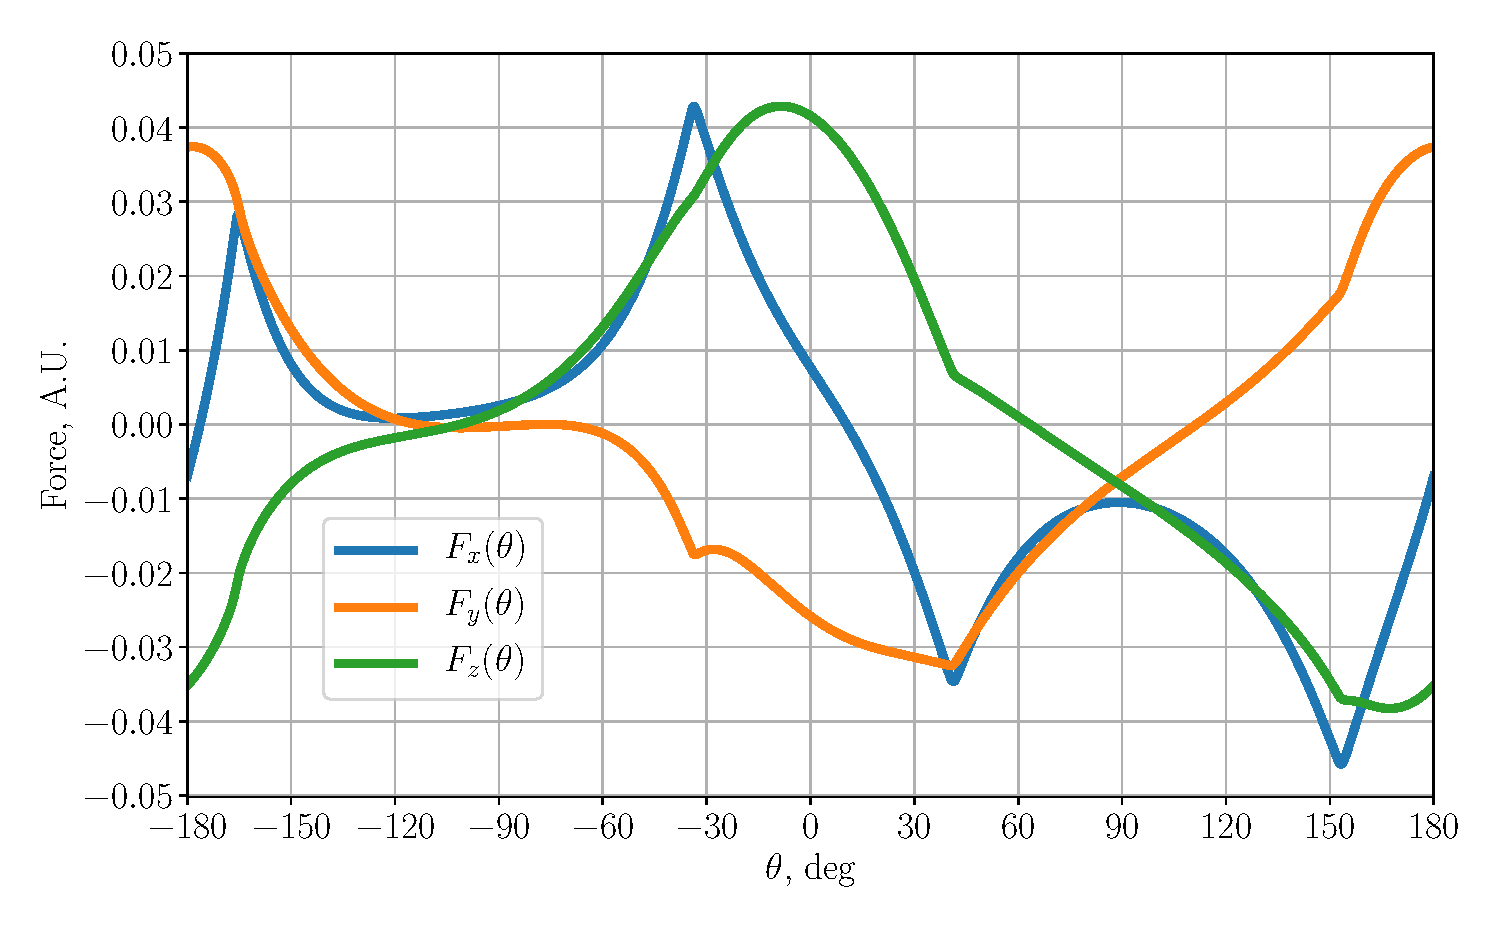
\includegraphics[width=0.45\linewidth]{ftot_rotation_lin_rect.pdf}}
    ~
    \subfloat[]{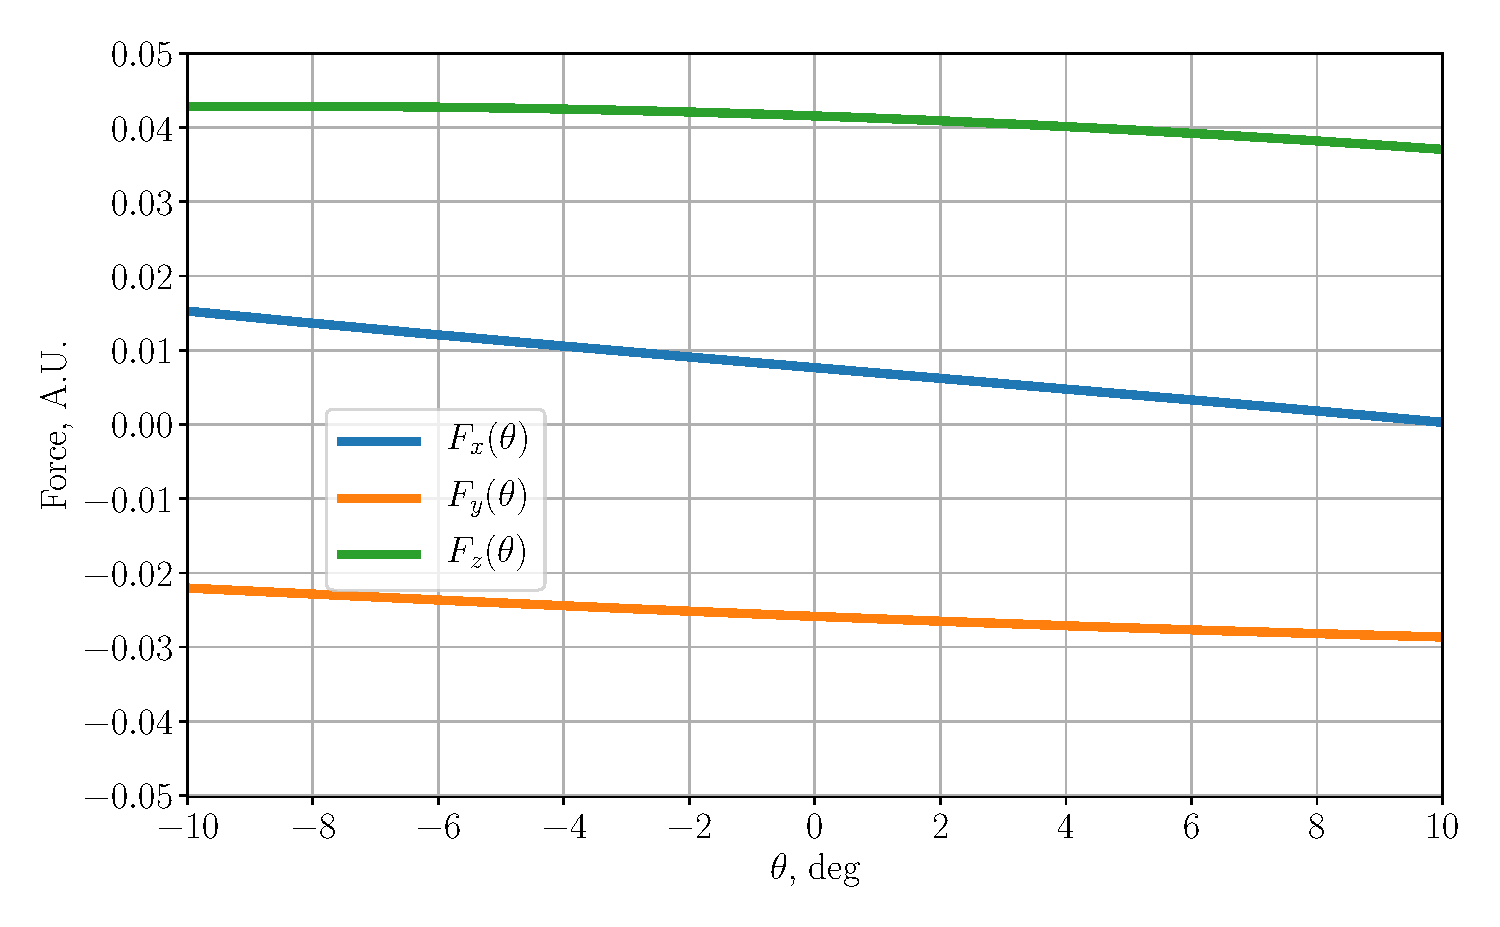
\includegraphics[width=0.45\linewidth]{ftot_rotation_lin_rect_zoom.pdf}}
    % \includegraphics[width=0.8\linewidth]{ftot_rotation_lin_rect_inlaid.pdf}
    \caption[Sample analytical forces on an element as a function of angle between surface and segment.]{(a) Example of the components of the total force on a surface element (the force summed over all four FE nodes) as a dislocation segment parallel to the surface element ($\theta = 0$) is rotated about its midpoint around the axis defined by $\vec{l}\times\vec{n}$. (b) is a zoomm into $\pm 10 \deg$, the force is smooth but not necessarily antisymmetric about the neighbourhood of $\theta=0$.}
    \label{f:rotate}
\end{figure}
The specific shape of the curves will vary depending on the element-segment configuration, but is smooth and well-behaved about singularity. For our purposes, we use a total of 8 perturbations of $1\deg$ each (4 clockwise and 4 anti-clockwise). We found this worked well, but can be changed if desired.

However, under finite-precision arithmetic, the check for orthogonality is dependent on the length scales involved in the simulation. This is particularly important considering the aforementioned use of arctangents, hyperbolic arctangents, logarithms and the large number of recurrence relations. Causing unexpected and rampant error propagation and numerical blow up is not difficult to achieve. When it happens, finding the root cause can lead one on a wild goose chase that is best avoided and often leads to a single segment in a single step of a long simulation that is slightly too small compared to its distance to a surface element to which it is slightly too parallel. To avoid these rare but high impact scenarios, we created a heuristic that dictates how strict the tolerance should be in order for the code to consider a segment to be parallel,
%
\begin{align}
    \lvert\vec{l}\cdot\vec{n}\rvert \lesssim \max\left(\lvert\vec{R}\cdot\vec{n}\rvert\right) \cdot 10^{-8}\,.
\end{align}
%
In our case we assume $\max\left(\lvert\vec{R}\cdot\vec{n}\rvert\right)$ to be the largest diagonal in our cuboid domain. A factor of $10^{-8}$ is used instead of actual machine precision $\sim10^{-15}$ because the seed functions and large number of recurrence relations of the solution propagate errors if the value of $\vec{l} \cdot \vec{n}$ is too close to zero. Ironically, tolerances which are too large can cause the perturbations to rotate the dislocation segment closer to the singularity, producing erroneous results. Larger than necessary tolerances can also slow down the calculation by detecting dislocations that are far enough from the special case that they can be treated like non-parallel segments. This heuristic is a good general purpose rule that keeps the tolerance in a goldilocks zone.

Another issue with the rotation is that one does not want a dislocation segment to intersect the surface when it is being rotated. Naively one would calculate the maximum rotational angle, $\theta_{\textrm{max}}$, to be,
%
\begin{align}
    \theta_{\textrm{max}} & = \arctan\left(\dfrac{2 d}{\left\lvert\vec{x_2} - \vec{x_1}\right\rvert}\right)\,.
\end{align}
%
Where $d$ is the minimum orthogonal distance from the dislocation to the surface element i.e. the collision distance---which in our case is a function of the dislocation core radius---and $\vec{x_1},\,\vec{x_2}$ are the dislocation segment node coordinates---whose maximum and minimum lengths are also functions of the dislocation core radius. However, $\theta_\textrm{max}$ might be too small in cases where the segment length is too small compared to the distance to a surface element, or when the segment length is much greater than $d$. Fine-tuning the angle is a task that involves knowing the minimum collision distance, minimum segment length, dislocation core radius, and the compiler's implementation of mathematical functions. Given the rarity of such cases and their comparatively low impact, we chose our $1\deg$ perturbation such that we safely avoid this problem while keeping within the bounds of the non-singular model.

Furthermore, the chirality and self-consistency of the FE nodes must be accounted for such that they are in the proper order regardless of the element face they belong to. Here we use 8-node linear hexahedral (brick) elements. The node ordering for the various surfaces is that for which the calculated normals point out from the domain, this is dependent on the specific FE mesh implementation.

The total force on a given node must include the force contributions from every element in which said node appears, see \cref{f:shared_node}.
\begin{figure}
    \centering
    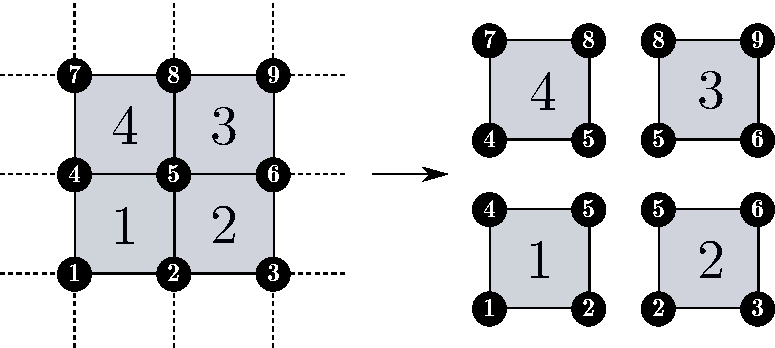
\includegraphics[width=\linewidth]{lrse_thread_map.pdf}
    \caption[FE nodes are shared between surface elements.]{FE nodes are shared by either 4 element faces or 3 if it is a corner node. The total force on a given node is the summation of the force contributions from each element it belongs to.}
    \label{f:shared_node}
\end{figure}
The specifics of the mapping depend on the global FE node numbering. Using \cref{f:shared_node} as our reference labels for elements and nodes, $e$ and $n$ respectively, we can give a concrete example of how this is done by defining,
\begin{subequations}
    \begin{align}
        \vec{f_{e,n}} & \coloneqq	\begin{bmatrix}
            f_{x_{e,n}} & f_{y_{e,n}} & f_{z_{e,n}}
        \end{bmatrix}^{\mathsf{T}}, \quad
        \vec{f_{n}} \coloneqq	\begin{bmatrix}
            f_{x_{n}} & f_{y_{n}} & f_{z_{n}}
        \end{bmatrix}^{\mathsf{T}}            \\
        \begin{split}
            \mtx{N_{L}} &=	\begin{bmatrix}
                l_{1,1} & l_{1,2} & l_{1,4} & l_{1,5} \\
                l_{2,2} & l_{2,3} & l_{2,5} & l_{2,6} \\
                l_{3,5} & l_{3,6} & l_{3,8} & l_{3,9} \\
                l_{4,4} & l_{4,5} & l_{4,7} & l_{4,8} \\
            \end{bmatrix}
        \end{split}
        , \quad
        \vec{\gamma} =   \begin{bmatrix}
            l_1    \\
            l_2    \\
            \vdots \\
            l_9
        \end{bmatrix}                             \\
        \begin{split}
            \mtx{F_{e}} &=	\begin{bmatrix}
                \vec{f_{1,1}} & \vec{f_{1,2}} & \vec{f_{1,4}} & \vec{f_{1,5}} \\
                \vec{f_{2,2}} & \vec{f_{2,3}} & \vec{f_{2,5}} & \vec{f_{2,6}} \\
                \vec{f_{3,5}} & \vec{f_{3,6}} & \vec{f_{3,8}} & \vec{f_{3,9}} \\
                \vec{f_{4,4}} & \vec{f_{4,5}} & \vec{f_{4,7}} & \vec{f_{4,8}} \\
            \end{bmatrix}
        \end{split}
        ,\quad
        \vec{\tilde{F}} = 	\begin{bmatrix}
            \vec{f_{1}} \\
            \vec{f_{2}} \\
            \vdots      \\
            \vec{f_{9}}
        \end{bmatrix}\,.\label{eq:force_imp}
    \end{align}
\end{subequations}
Where $\vec{f_{e,n}}$ is a $3\times1$ column vector corresponding to the $(x\,,y\,,z)$ dislocation induced forces on node, $n$, on the surface element, $e$. There are four of these per rectangular surface element. Any given node, $n$, can appear in multiple surface elements (e.g. node 5 in \cref{f:shared_node} is shared by all 4 surface elements), all of which independently contribute to the total force on said node. $\vec{f_n}$ is a $3\times1$ column vector corresponding to the total dislocation induced forces on node $n$. These are used to shorten the definition of \cref{eq:force_imp} and are not explicitly defined in the implementation, rather they give the force matrices $\mtx{F_{e}}$ and $\vec{\tilde{F}}$ a specific row order. $\mtx{N_{L}}$ is crucial for the correct implementation of this analytical solution in traditional FE codes. It is the $E\times4$ matrix corresponding to the global label of each node in a given surface element. Each row of the matrix represents a surface element and each column represents a node in the surface element. We cannot na\"ively add the columns together as that would give the total force acting on the element as a whole, not each FE node individually. We chose to arrange the columns in accordance to \cref{f:force_lin_rect} as it makes it easier to implement the solution, but the only thing that matters is that the basis vectors $\vec{n},\,\vec{p},\,\vec{q}$ are calculated appropriately. $\vec{\gamma}$ is the vector with the FE node labels, which makes mapping force to node possible. $\mtx{F_{e}}$ is the $3E \times 4$ matrix where the forces acting on each of the four nodes (column) in a particular surface element (each element corresponds to three consecutive rows because there are three dimensions) are stored. $\vec{\tilde{F}}$ is the $3N\times1$ column vector where the total forces on each node are stored (each node has three rows because there are three dimensions). This is easily generalisable to $E$ elements and $N$ nodes.

\Cref{a:tot_force} illustrates how the total force on each node is obtained. However, our implementation does not strictly follow it because we memoise a generalised version of $\vec{L}$ upon simulation initialisation instead of finding one at every iteration, reducing computational time but requiring us to account for nodes without traction boundary conditions. Our indexing also starts at 1, but zero indexing makes the algorithm easier to follow.
\begin{algorithm}
    \caption[Calculating total force on a node using analytic tractions.]{Assuming $ \vec{\tilde{F}} $ is arranged the same way as $ \vec{\gamma} $ and indexing starts at 0.}
    \begin{algorithmic}[1]
        \label{a:tot_force}
        \State\Comment{Loop through the array containing the node labels of the relevant surface nodes.}
        \For{$ i = 0;\, i < \rvar{length}(\vec{\gamma});\, i++$}					\State\Comment{Save the global node label for the current iteration.}
        \State $ n \gets \vec{\gamma}[i] $
        \State\Comment{Use the node label to find a vector, $\vec{L}$, with the linearised indices in $\mtx{N_{L}}$ where node $n$ appears as part of a surface element whose tractions we are calculating.}
        \State $ \vec{L} \gets \rvar{find}(\mtx{N_{L}} == n) $
        \State\Comment{Loop over coordinates.}
        \For{$ k = 0;\, k < 3;\, k++ $}
        \State\Comment{Use global node label vector to index the force array from the analytical force calculation. Multiplied by 3 because there are three coordinates per node. We sum the forces from the analytical calculation because the same global node can be part of multiple surface elements. We add $ k $ because the $ x,~y,~z $ coordinates are consecutively stored in $ \mtx{F_{e}} $.}
        \State $ \vec{\tilde{F}}[3n + k] \gets \vec{\tilde{F}}[3n + k] + \sum\mtx{F_{e}}[3\vec{L} + k]  $
        \EndFor
        \EndFor
    \end{algorithmic}
\end{algorithm}

The resulting force vector is then used in \cref{eq:thatbc} to calculate $\tns{\hat{\sigma}}$, since $\tilde{\vec{T}} \coloneqq \tilde{\vec{F}}$. \Cref{f:headvstractionfem} shows the simple system we used to compare the image stresses calculated by our FE solver using numeric tractions v.s. analytic tractions v.s. infinite-domain, singular image stresses in \cref{eq:imageStressAnalyticEdge1,eq:imageStressAnalyticEdge2,eq:imageStressAnalyticScrew}. The three test cases are: two edge dislocations and one screw, all of which have line direction $\vec{l} = [0\, 0\, 1]$. The Burgers vectors for the different scenarios are $\vec{b}_\textrm{e1} \coloneqq \vec{b} = [1\, 0\, 0]$, $\vec{b}_\textrm{e2} \coloneqq \vec{b} = [0\, 1\, 0]$, as defined in \cite{head1953edge}; and $\vec{b}_\textrm{s} \coloneqq \vec{b} = \vec{l} = [0\, 0\, 1] $, and therefore $b \coloneqq \lVert \vec{b} \rVert = 1$ as defined in \cite[p.~59,~64]{hirth1983theory}. The units in all our examples are normalised to lattice parameter.

\begin{figure}
    \centering
    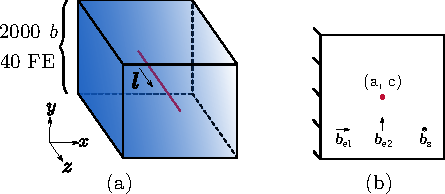
\includegraphics[width=0.8\linewidth]{head_vs_fe_tractions_setup_diagram.pdf}
    \caption[Set up comparing infinite-domain, singular solutions of stress fields to those obtained via a non-singular formulation with analytic and numeric tractions coupled to FEM.]{Dislocation parallel to a surface described by the line $x = 0$, where the $(x,\,y)$ dislocation coordinates are $(a,\,c)$ and the dislocation line going in the positive $z$-direction. (a) describes the box we used for our comparison, a  $40 \times 40 \times 40$ element cubic box with side lengths equal to $2000$ with $\vec{T} = \bm{0}$, traction boundary conditions only on the nodes along $x = 0$, and $\vec{U} = \bm{0}$, displacement conditions everywhere else. (b) is the 2D view with the dislocation coordinates $(a,~c)$, as well as the two edge Burgers vectors in \cite{head1953edge}, $\vec{b}_\textrm{e1} \coloneqq \vec{b} = [1\, 0\, 0]$, $\vec{b}_\textrm{e2} \coloneqq \vec{b} = [0\, 1\, 0]$ and the screw Burgers vector $\vec{b}_\textrm{s} \coloneqq \vec{b} = \vec{l} = [0\, 0\, 1] $ in \cite[p.~59,~64]{hirth1983theory}.}
    \label{f:headvstractionfem}
\end{figure}

The slices we took for our contour plots in \cref{ss:paperResults} are on the middle plane of the domain at $z = 1000$.

We also ran a very simple simulation comparing the results between using analytic tractions as opposed to numeric ones. Finding a simple yet clear case of tractions producing catastrophically wrong behaviours can be difficult. Large differences in image forces are relatively rare and other factors often dominate. Such factors include the core radius---which affects the dislocation line tension and therefore works against the deformation of a dislocation line---mobility law and mobility parameters used, external loading, etc.

However, we found a simple and realistic configuration that is close to the setup in the infinite domain examples. The differences between those comparisons and the simulation are described in \cref{t:simulation_params}. We use a mobility law developed in-house by B. Bromage \cite{bromage2018calculating}, that corrects common issues found in other laws. We also rotate the domain such that the $[1\, 1\, 1]$ and $[1\, \overline{1}\, 0]$ crystallographic directions respectively correspond to the simulation's $x$ and $y$-directions, for this we use the same rotation technique as \cite{YU2018}. The dislocation was allowed to move under no external loads or displacements, with $\vec{T} = \bm{0}$ boundary conditions only on the $yz$-plane and $\vec{U} = \bm{0}$ everywhere else.
\begin{table}
    \centering
    \caption[Numeric v.s. analytic tractions. Unloaded simulation comparison.]{Parameters for our simulation. Where $\mtx{R}$ is a rotation matrix such that the $\vec{x},\, \vec{y},\, \vec{z}$ basis vectors of our simulation correspond to the $\vec{b},\, \vec{n},\, \vec{l}$ crystallographic directions. As these are row rather than column vectors, the rotation is transposed to what is traditional, i.e. $\vec{x}\mtx{R} = \vec{b}$. All values are in units of lattice parameters.}
    \label{t:simulation_params}
    \begin{tabular}{ll}
        \toprule
        Parameter                & Value                                                     \\
        \midrule
        Crystal Structure        & BCC                                                       \\
        Lattice size, $a$        & $3.18\times 10^{-4}~\mu\text{m}$                          \\
        $\vec{b}$                & $\frac{1}{2}[1\, 1\, 1]$                                  \\
        $\vec{n}$                & $[1\, \overline{1}\, 0]$                                  \\
        $\vec{l}$                & $[1\, 1\, \overline{2}]$                                  \\
        $b$                      & $\sqrt{3}/2\, a$                                          \\
        Core radius, $r_a$       & $5\, a$                                                   \\
        Grid Size                & $20 \times 20 \times 20$ elements                         \\
        Cubic domain side length & $2000\, a $                                               \\
        $(x_{0},\, y_{0})$       & $(62.5,\, 1000)\, a$                                      \\
        Min segment length       & $50\, a$                                                  \\
        Max segment length       & $125\, a$                                                 \\
        $\mtx{R}$                & $\begin{bmatrix} \hat{\vec{b}} \\ \hat{\vec{n}} \\ \hat{\vec{l}} \end{bmatrix} = \begin{bmatrix} \sqrt{3}/3 & \sqrt{3}/3 & \sqrt{3}/3 \\ \sqrt{2}/2 & -\sqrt{2}/2 & 0 \\ \sqrt{6}/6 & \sqrt{6}/6 & -\sqrt{6}/3\end{bmatrix}$ \\
        \bottomrule
    \end{tabular}
\end{table}

\subsection{Results and discussion}\label{ss:paperResults}

\Cref{f:rel_err_perp_edge} shows that even for dislocations only one dislocation core radius ($5$) away from the surface element, the force can be obtained, up to numerical precision, with 1000 Gauss quadrature points $Q$ for all segment lengths tested. It also shows a very peculiar issue Gauss quadrature has when computing integrals of rational functions when the Gauss nodes are close poles/maximal values. This undesirable behaviour is observed in the case where $Q = 11$. Where the highest weighted Gauss node is closest to the point where $1/R_{a}$ is maximal, resulting in lower accuracy when compared to $Q = 2, 10$ in \cref{f:rel_err_perp_edge} (a) and (b).
\begin{figure}
    \centering
    \subfloat[Segment starts a single dislocation core radius away.]
    {
        {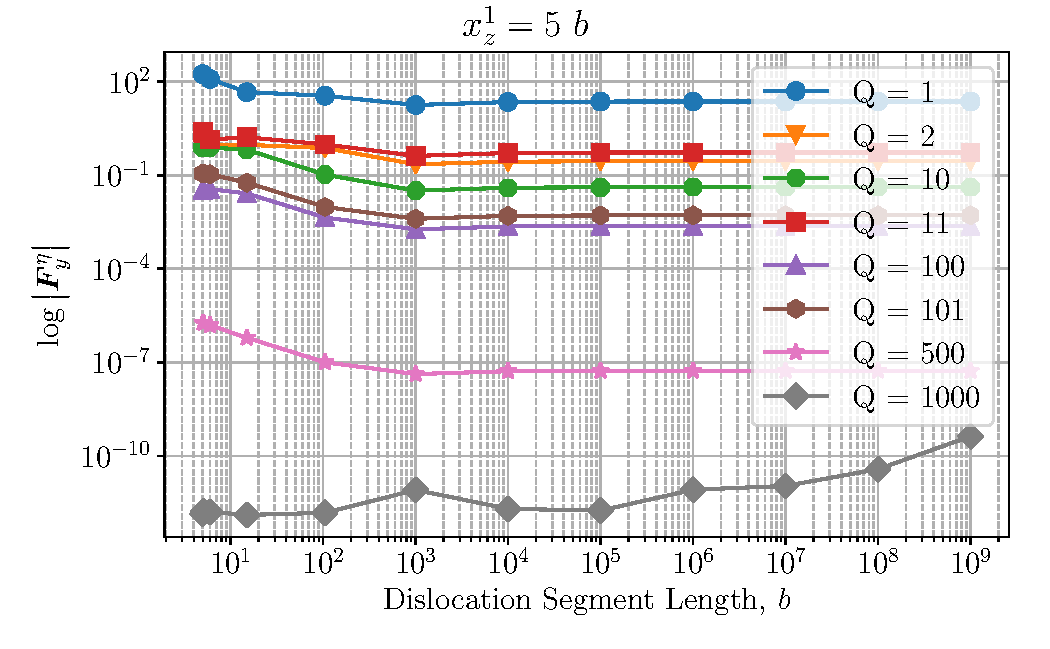
\includegraphics[trim={0.5cm 0.55cm 0.65cm 0.1cm},clip,width=0.475\linewidth]{perp_e_xz=5.pdf}}
    }
    ~
    \subfloat[Segment starts 3 dislocation core radii away.]
    {
        {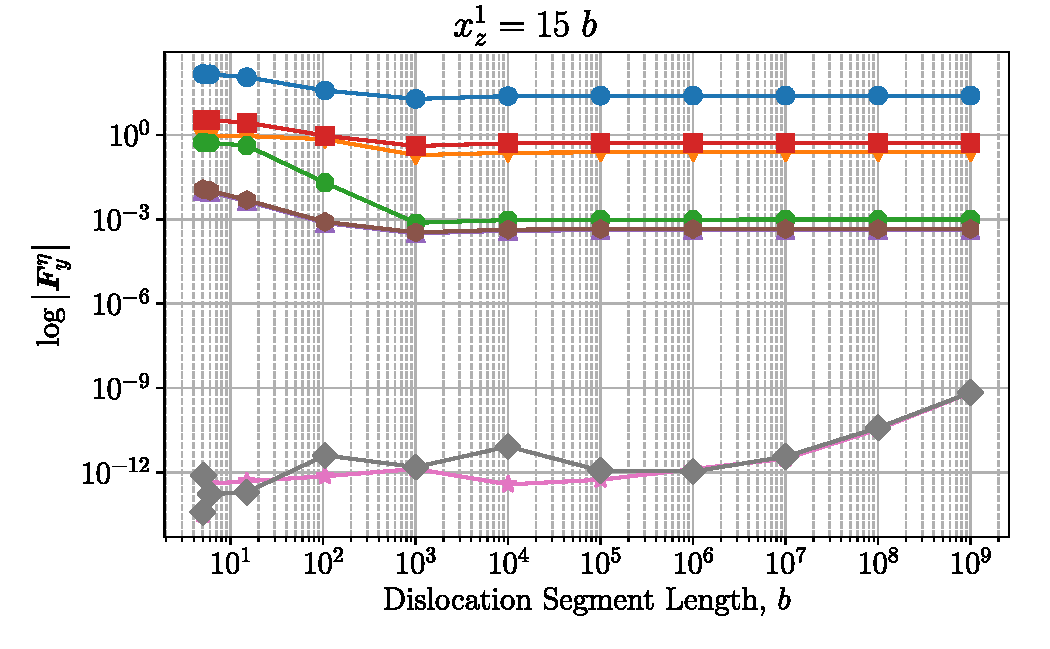
\includegraphics[trim={0.5cm 0.55cm 0.65cm 0.1cm},clip,width=0.475\linewidth]{perp_e_xz=15_leg.pdf}}
    }

    \subfloat[Segment starts 201 dislocation core radii away.]
    {
        {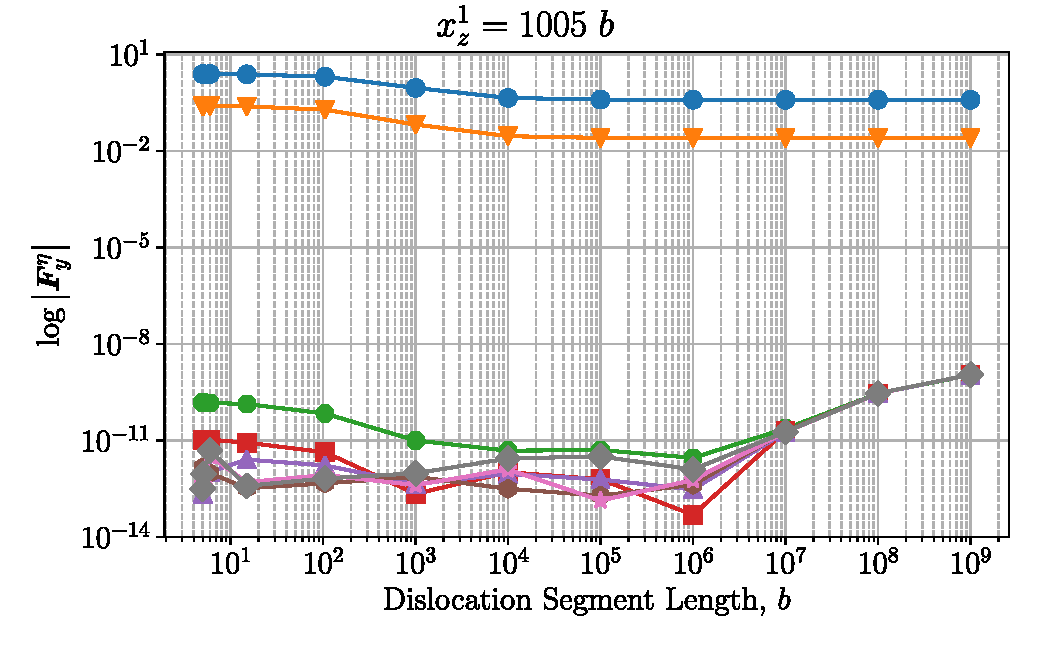
\includegraphics[trim={0.5cm 0.55cm 0.65cm 0.1cm},clip,width=0.475\linewidth]{perp_e_xz=1005_leg.pdf}}
    }
    ~
    \subfloat[Segment starts 20001 dislocation core radii away.]
    {
        {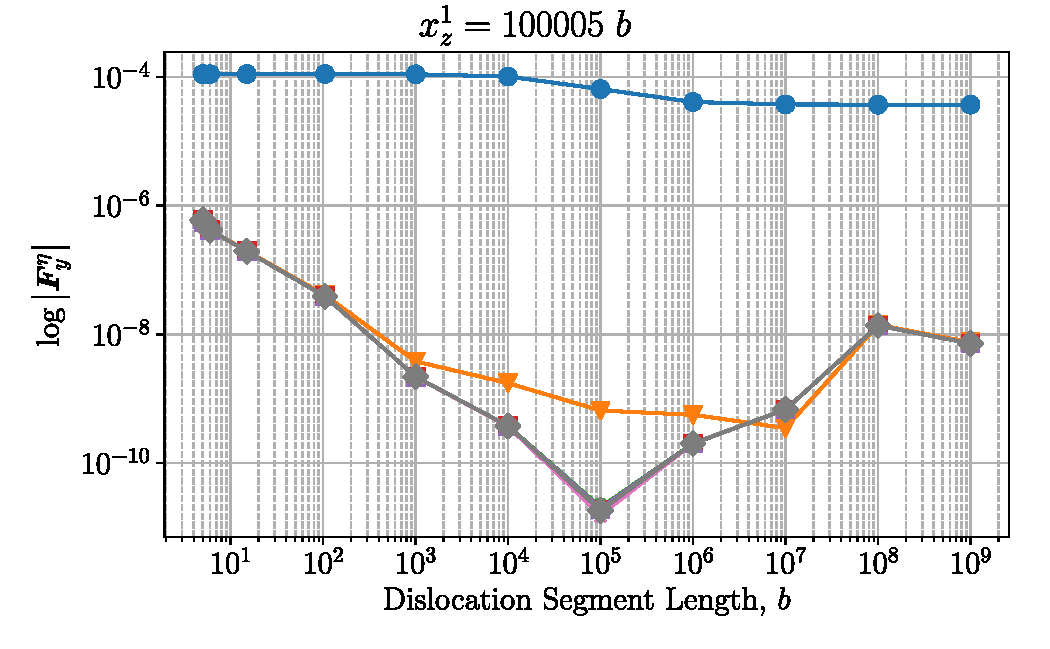
\includegraphics[trim={0.5cm 0.55cm 0.65cm 0.1cm},clip,width=0.47\linewidth]{perp_e_xz=100005_leg.pdf}}
    }
    \caption[Relative error for an edge dislocation perpendicular to a surface element.]{Log-log plot of the relative error as a function of dislocation segment length for a perpendicular edge dislocation (\cref{f:gauss_quad_test}a). $x^{1}_{z}$ is the $z$-coordinate of node $\vec{x_1}$. $\vec{b} = [1\, 0\, 0]$, line direction, $\vec{l} = [0\, 0\, 1]$, and dislocation core radius, $a = 5$, the surface element's normal and size are, $\vec{n} = [0\, 0\, 1]$, $L = 1000$, respectively. $Q$ is the number of quadrature points per dimension.}
    \label{f:rel_err_perp_edge}
\end{figure}
It is worth noting however that the relative errors for small numbers of quadrature points don't really start decreasing until relatively large distances. And when close to a surface, these can be quite large even under highly symmetric circumstances.

The limitations become even more evident when the dislocation line segment is parallel to a surface element. In \cref{f:rel_err_par_edge}, we observe the relative errors are quite large when close to the surface. At distances larger than $10^4$, loss of significance causes the relative errors to converge at $\sim 1$ which is expected as two finite precision floating point numbers get closer to zero. Of particular note is how large the relative errors are even at $100$ lattice units away from the surface, even for large numbers of quadrature points. This figure backs up the earlier point regarding Gauss nodes close to maximal values of rational functions. It can be shocking to see that as $Q = 2$ performs significantly better than $Q = 10, 11, 100, 100$ at distances from the surface as having nodes near the maximal values is a large source of error. Consequently, different configurations have different optimal numbers of points. The numerical instability of this method, which when coupled to the chaotic nature of dislocation dynamics and stiffness of the equations of motion, can lead to large deviations between simulations.
\begin{figure}
    \centering
    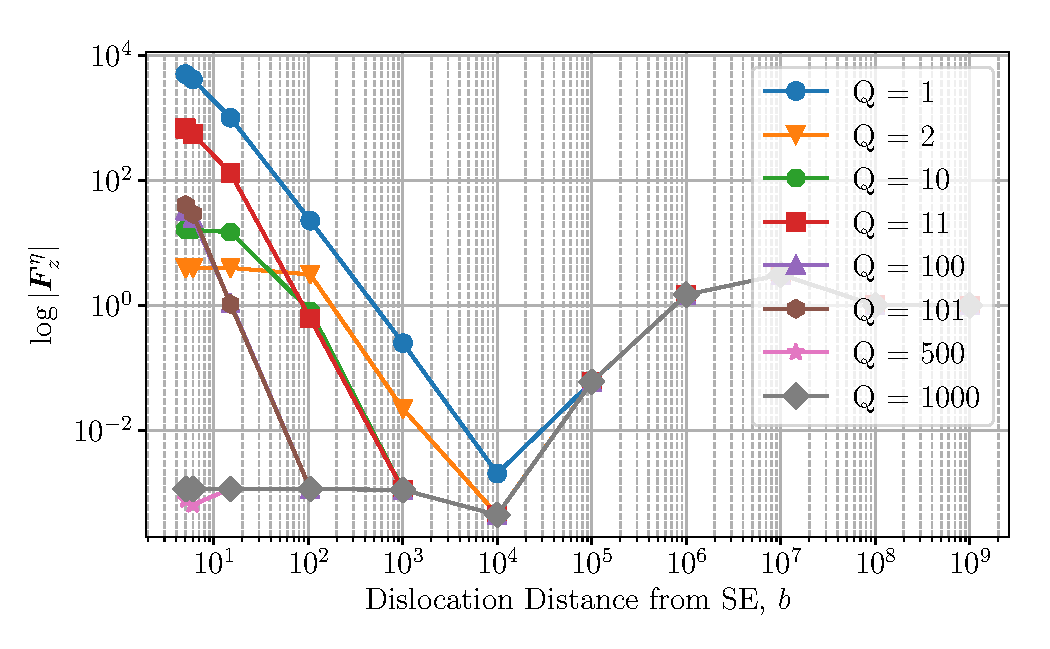
\includegraphics[width=0.8\linewidth]{par_e_z.pdf}
    \caption[Relative error for an edge dislocation parallel to a surface element.]{Log-log plot of the relative error as a function of distance from the surface element for a parallel edge dislocation (\cref{f:gauss_quad_test}b). Burgers vector, $\vec{b} = [0\, 1\, 0]$, line direction, $\vec{l} = [1\, 0\, 0]$, dislocation core and surface element parameters are the same as \cref{f:rel_err_perp_edge}. The dislocation length is fixed to $10^{6},\, x\in\left[-0.5\times10^{6},\, 0.5\times10^{6} \right]$ and bisects the surface element along the $[1\, 0\, 0]$ direction. The whole dislocation was segmented into $10^4$ pieces of length $100$ to prevent the dislocation from intersecting the surface element when they were rotated to avoid the singularity. The relative error at large distances ($>10^6$) converges to one due to loss of significance.}
    \label{f:rel_err_par_edge}
\end{figure}

From \cref{f:rel_err_perp_edge,f:rel_err_par_edge} one might be tempted to say that for a segment parallel to a surface, Gauss quadrature performs far worse than for a perpendicular one. However, there is a further wrinkle in this problem: symmetry. To exemplify this we plot the relevant components of the stress tensor for the arrangement found in \cref{f:gauss_quad_test}(a) in \cref{sf:xzeperp,sf:yzeperp,sf:zzeperp}. The $\sigma_{xz}$ and $\sigma_{zz}$ components are antisymmetric about the centre of the element. If we use Gauss quadrature on them, we sample equivalent but oppositely valued points that are equally weighted, thus the sum vanishes and therefore do not contribute to \cref{f:rel_err_perp_edge}. However, $\sigma_{yz}$ does not vanish, but can be accurately integrated with sufficiently large $Q$. If we were to move the dislocation off-centre such that these symmetries are broken, the errors would increase.

We also plot the relevant stresses for the arrangement described by \cref{f:gauss_quad_test}(b) in \cref{sf:xzepar,sf:yzepar,sf:zzepar}. From \cref{sf:xzepar} and \cref{sf:yzepar}, it is immediately apparent why gauss quadrature fails so spectacularly in \cref{f:rel_err_par_edge}. At low numbers of quadrature points, it fails to appropriately sample the rapidly changing value of $\tilde{\sigma}_{xz}$ at both ends of the dislocation, as well those in the neighbourhood of the dislocation in $\tilde{\sigma}_{yz}$. Moreover, the further away the quadrature points are from the midpoint of the domain, the lower their relative weighting. So even with a relatively large number of them, there can still be large errors. Which is a particularly egregious problem in \cref{sf:yzepar}, and explains why so many quadrature points are required to accurately compute the integral.
\begin{figure}
    \centering
    \subfloat[\label{sf:xzeperp}]
    {
        {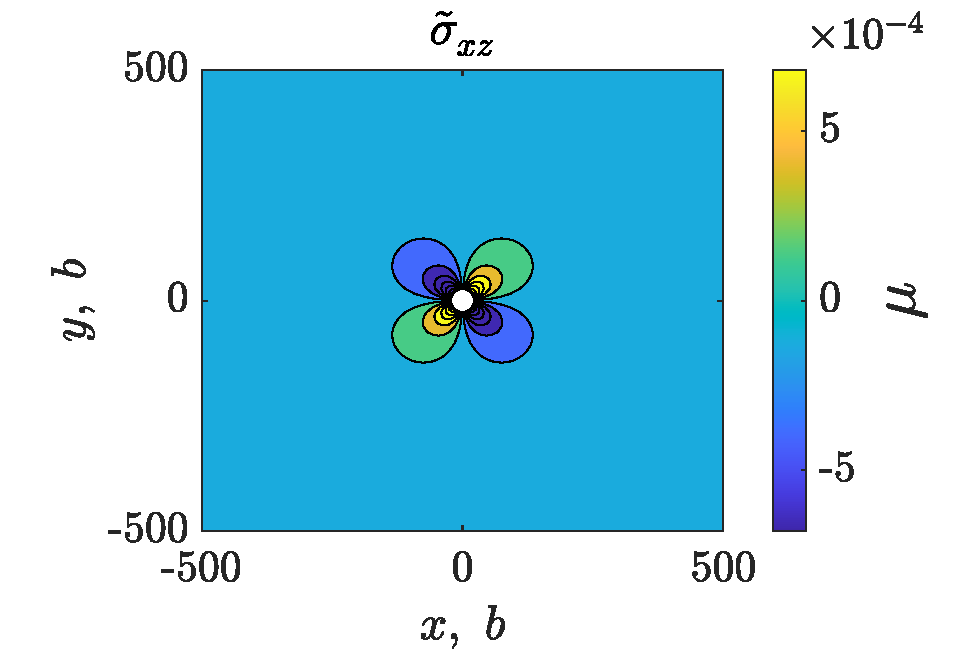
\includegraphics[trim={0.5cm 0cm 0cm 0cm},clip,width=0.3\linewidth]{sxzperpEdgeFiveb.pdf}}
    }
    ~
    \subfloat[\label{sf:yzeperp}]
    {
        {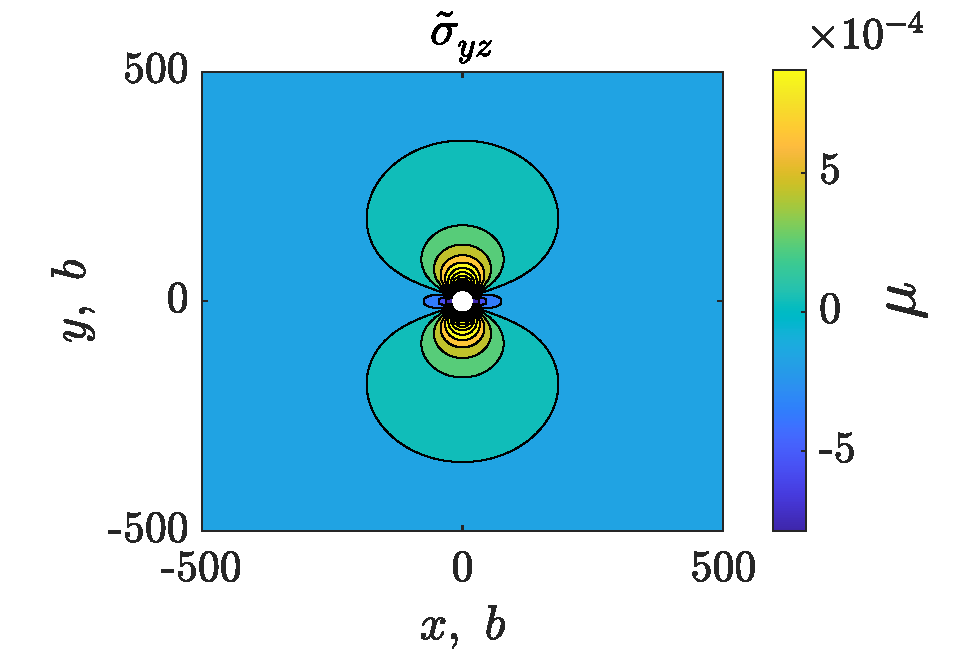
\includegraphics[trim={0.5cm 0cm 0cm 0cm},clip,width=0.3\linewidth]{syzperpEdgeFiveb.pdf}}
    }
    ~
    \subfloat[\label{sf:zzeperp}]
    {
        {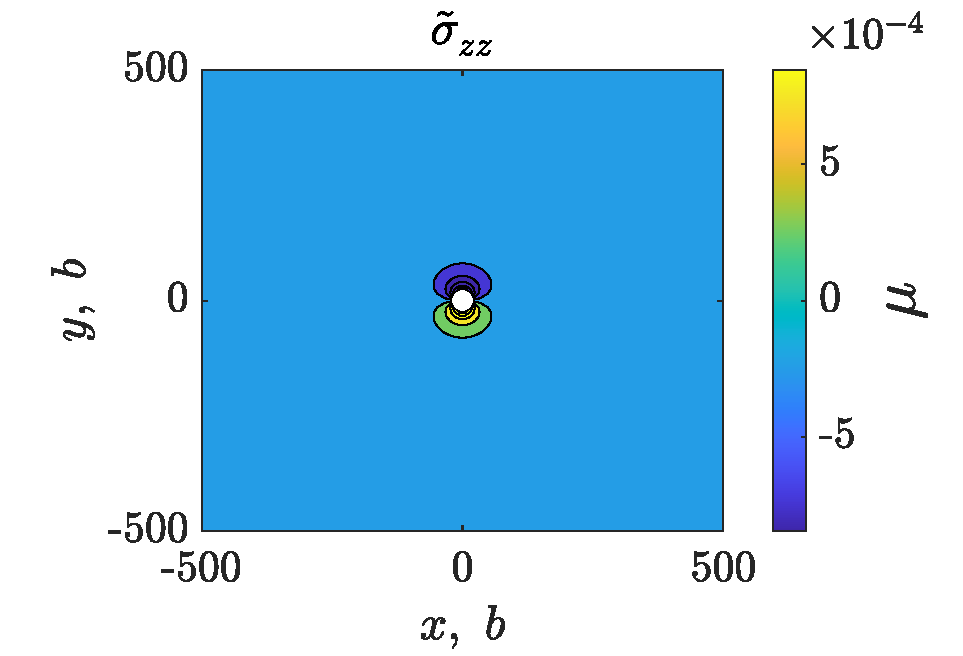
\includegraphics[trim={0.5cm 0cm 0cm 0cm},clip,width=0.3\linewidth]{szzperpEdgeFiveb.pdf}}
    }

    \subfloat[\label{sf:xzepar}]
    {
        {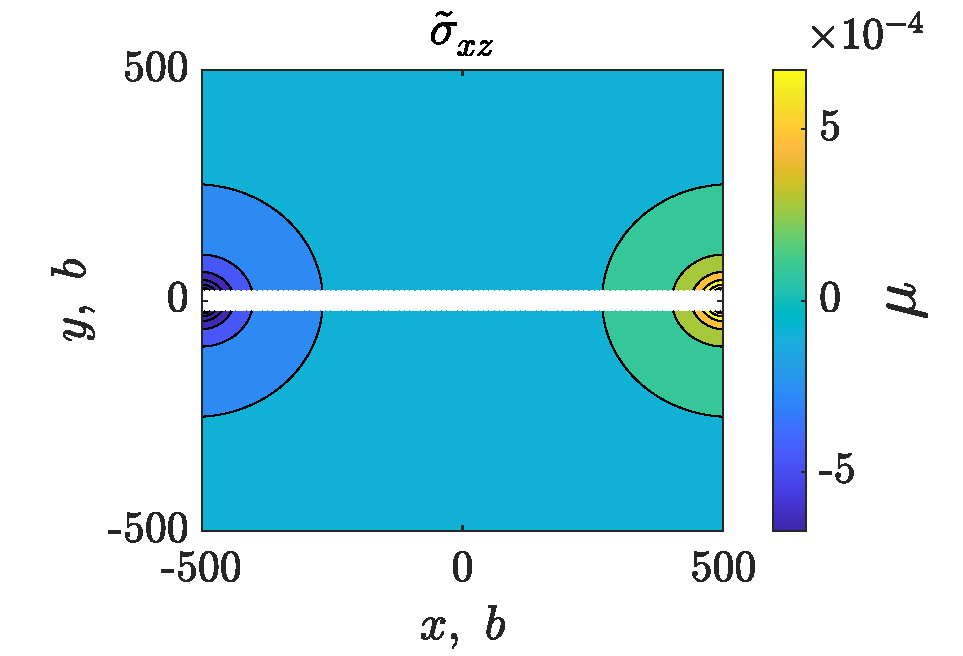
\includegraphics[trim={0.5cm 0cm 0cm 0cm},clip,width=0.3\linewidth]{sxzparEdgeFiveb.pdf}}
    }
    ~
    \subfloat[\label{sf:yzepar}]
    {
        {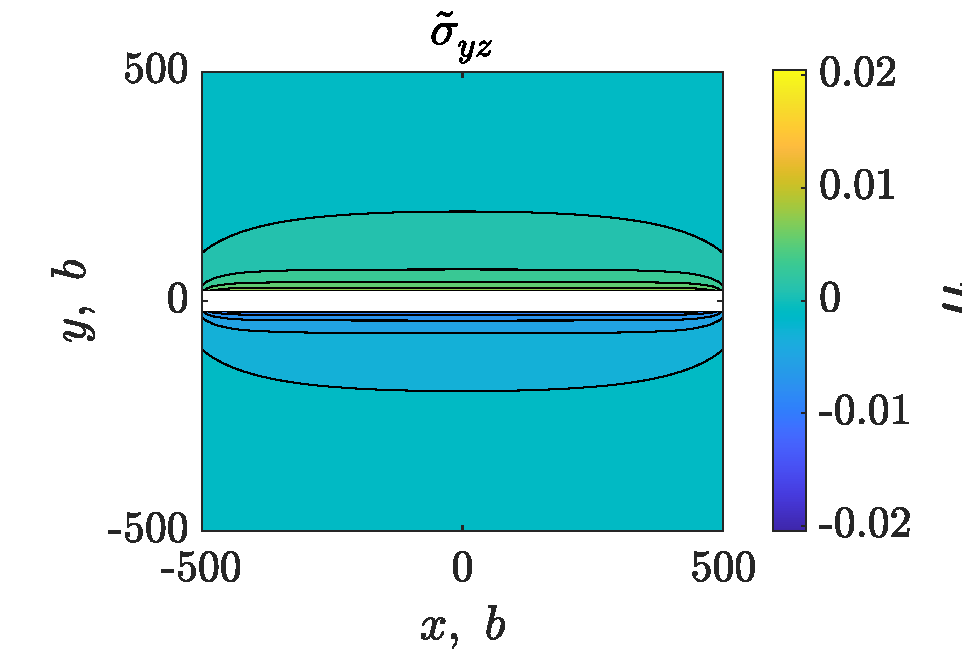
\includegraphics[trim={0.5cm 0cm 0cm 0cm},clip,width=0.3\linewidth]{syzparEdgeFiveb.pdf}}
    }
    ~
    \subfloat[\label{sf:zzepar}]
    {
        {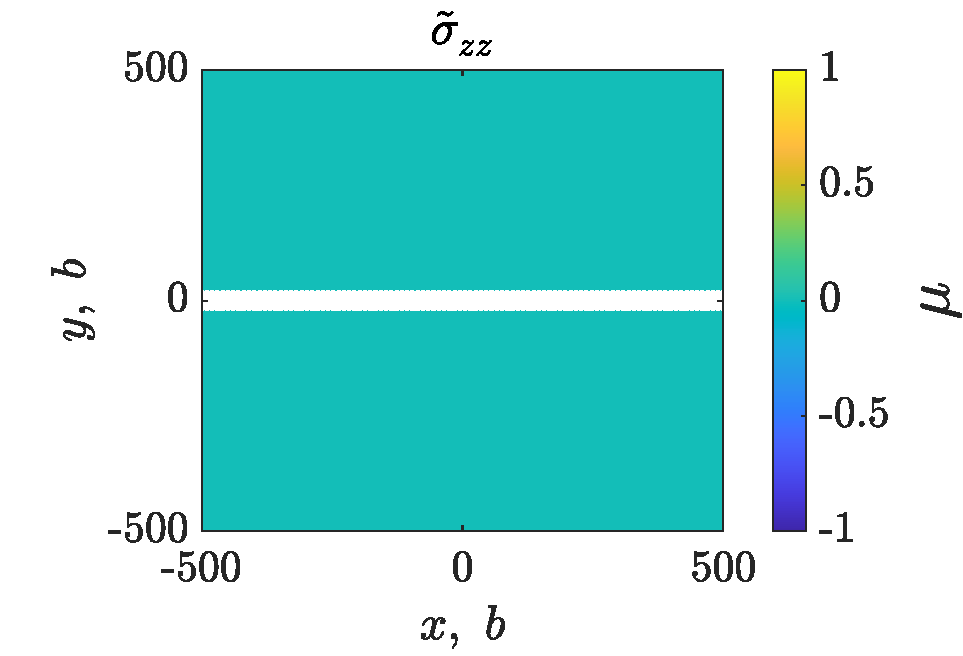
\includegraphics[trim={0.5cm 0cm 0cm 0cm},clip,width=0.3\linewidth]{szzparEdgeFiveb.pdf}}
    }
    \caption[Symmetry in stress fields leads more accurate numeric tractions.]{(a) to (c) show the real stress fields from a dislocation in the same configuration that yields the plots found in \cref{f:rel_err_perp_edge} as shown in \cref{f:gauss_quad_test}(a), where the closest node is a dislocation core radius away from the surface, $a = 5$. (e) to (f) does the same for the configuration that yields \cref{f:rel_err_par_edge} as shown in \cref{f:gauss_quad_test}(b), where the whole dislocation is a core radius away from the surface, $a = 5$. The white line or dot is the dislocation. Units are in terms of lattice parameters.}
    \label{f:sigma_edge_test_config}
\end{figure}

Despite these being artificially idealised examples that illustrate the failings of Gauss quadrature, other problematic scenarios commonly show up in simulations. These tend to worsen with smaller core radii $a$, fewer Gauss nodes, higher dislocation densities near surfaces, more permissive mobility functions, and coarser FE meshes. The $\mathcal{O}(1/R)$ decay rate of $\tns{\tilde{\sigma}}$ and chaotic nature of dislocation dynamics, means these errors may result in unwarranted topological changes that cascade as the simulation advances. This is particularly deleterious when doing simulations with higher dislocation densities and/or where numerous dislocations are close to the surface, such as nanoindentation simulations.

\begin{figure}
    \centering
    \subfloat[%$\hat{\sigma}_{xx}$.
        \hspace{-0.8cm}\label{sf:sxxeperp}]
    {
        {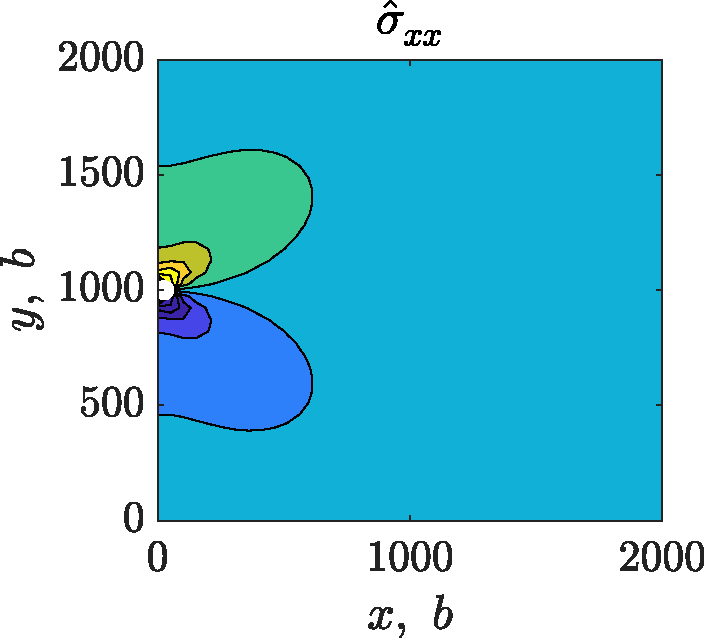
\includegraphics[width=0.25\linewidth]{sxxEperp_leg.pdf}}
    }~
    \subfloat[%$\hat{\sigma}^\textrm{A}_{xx}$.
        \hspace{-0.8cm}\label{sf:sxxAeperp}]
    {
        {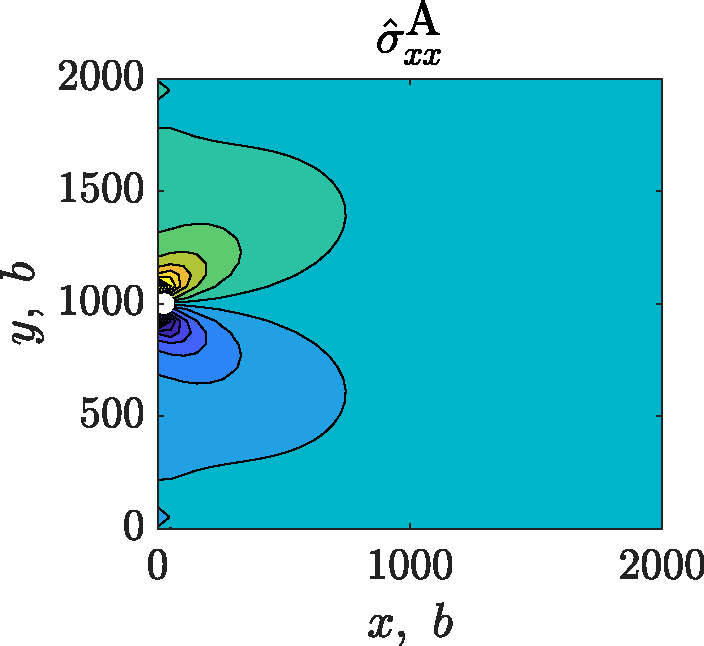
\includegraphics[width=0.25\linewidth]{sxxAEperp_leg.pdf}}
    }~
    \subfloat[%$\hat{\sigma}^\textrm{N}_{xx}$.
        \hspace{-0.8cm}\label{sf:sxxNeperp}]
    {
        {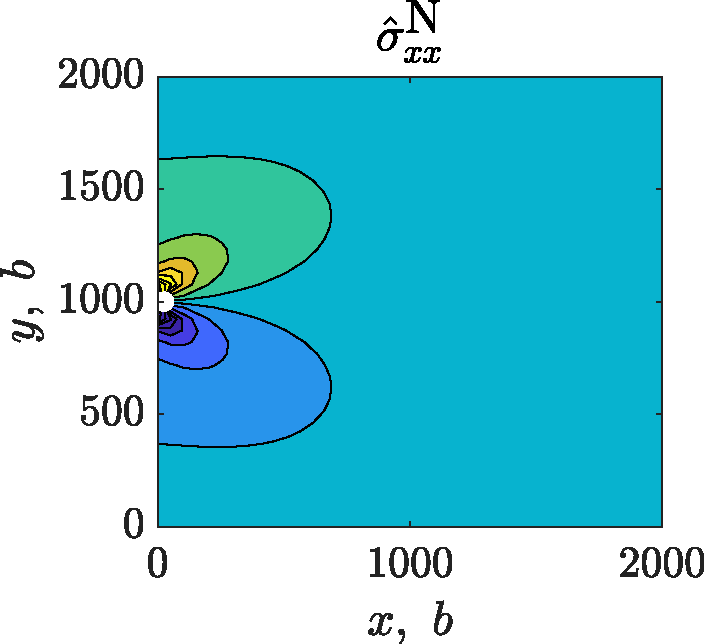
\includegraphics[width=0.25\linewidth]{sxxNEperp_leg.pdf}}
    }~
    \subfloat{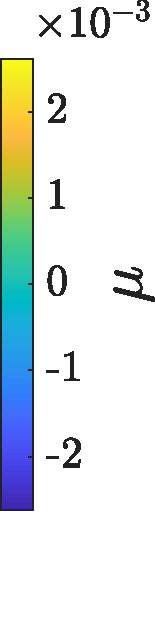
\includegraphics[height = 0.22\linewidth]{sxxNAEperp_leg.pdf}}

    \subfloat[%$\hat{\sigma}_{yy}$.
        \hspace{-0.8cm}\label{sf:syyeperp}]
    {
        {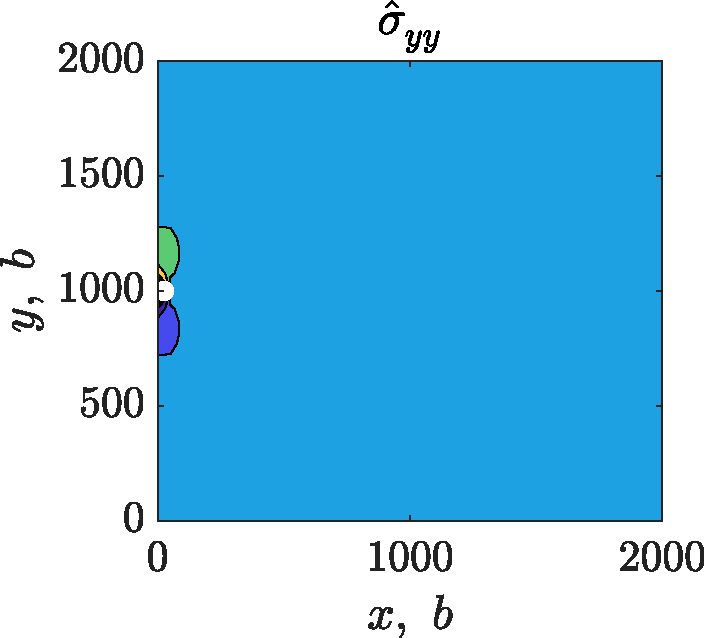
\includegraphics[width=0.25\linewidth]{syyEperp_leg.pdf}}
    }~
    \subfloat[%$\hat{\sigma}^\textrm{A}_{yy}$.
        \hspace{-0.8cm}\label{sf:syyAeperp}]
    {
        {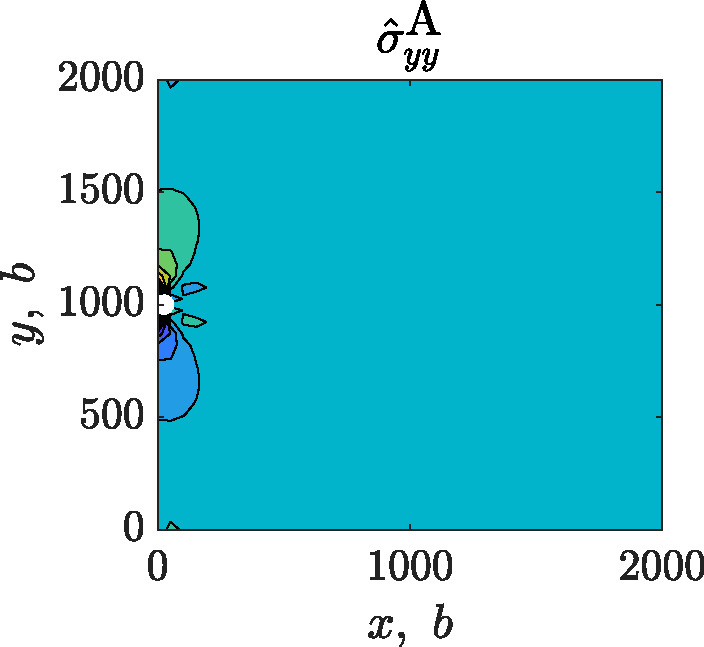
\includegraphics[width=0.25\linewidth]{syyAEperp_leg.pdf}}
    }~
    \subfloat[%$\hat{\sigma}^\textrm{N}_{yy}$.
        \hspace{-0.8cm}\label{sf:syyNeperp}]
    {
        {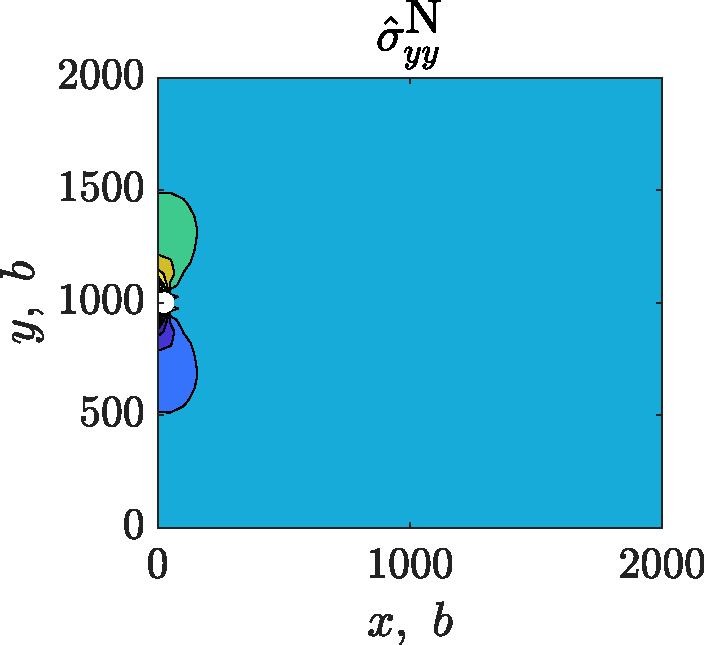
\includegraphics[width=0.25\linewidth]{syyNEperp_leg.pdf}}
    }~
    \subfloat{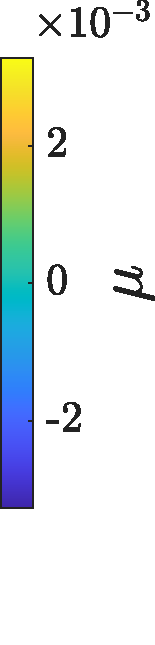
\includegraphics[height = 0.22\linewidth]{syyNAEperp_leg.pdf}}

    \hspace*{0.2cm}\subfloat[%$\hat{\sigma}_{xy}$.
        \hspace{-0.8cm}\label{sf:sxyeperp}]
    {
        {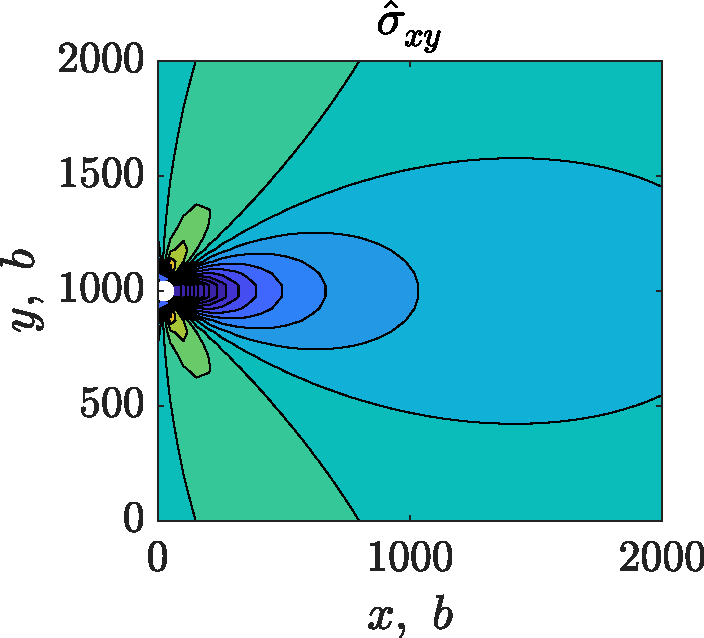
\includegraphics[width=0.25\linewidth]{sxyEperp_leg.pdf}}
    }~
    \subfloat[%$\hat{\sigma}^\textrm{A}_{xy}$.
        \hspace{-0.8cm}\label{sf:sxyAeperp}]
    {
        {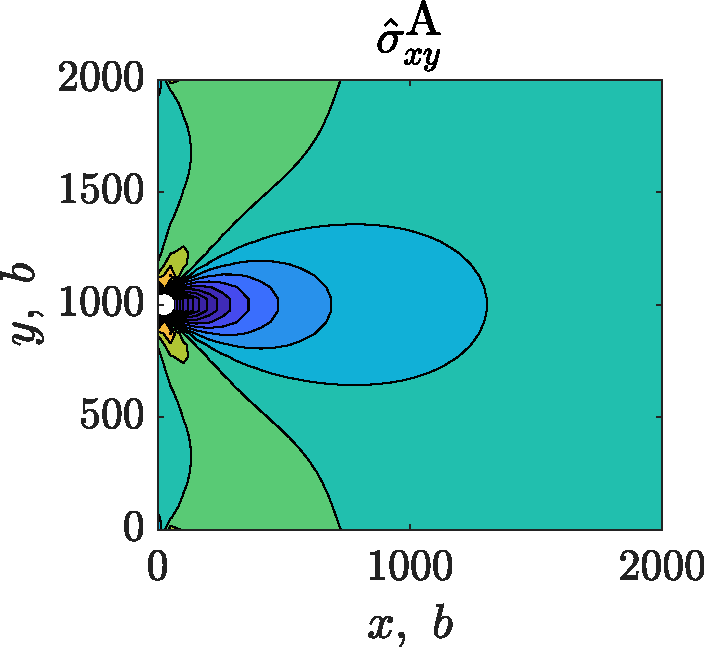
\includegraphics[width=0.25\linewidth]{sxyAEperp_leg.pdf}}
    }~
    \subfloat[%$\hat{\sigma}^\textrm{N}_{xy}$.
        \hspace{-0.8cm}\label{sf:sxyNeperp}]
    {
        {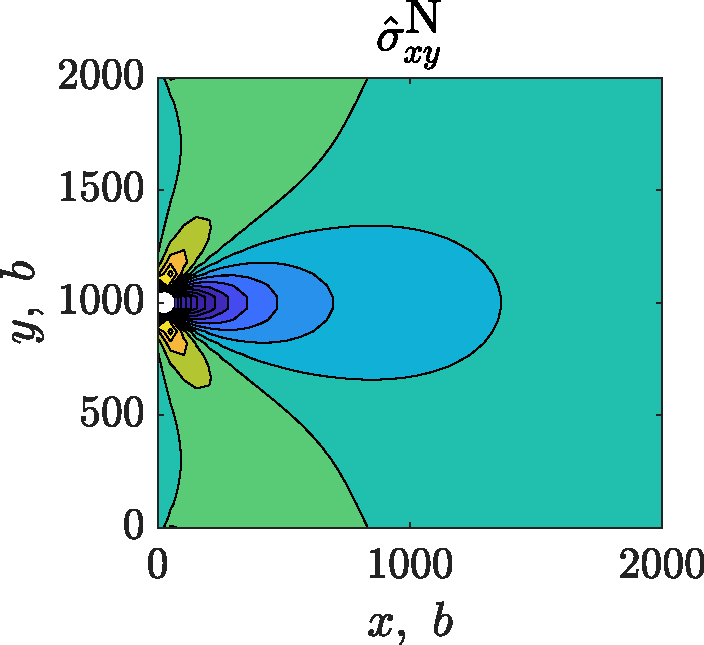
\includegraphics[width=0.25\linewidth]{sxyNEperp_leg.pdf}}
    }~
    \hspace*{-0.2cm}\subfloat{
        \includegraphics[height = 0.22\linewidth]{sxyNAEperp_leg.pdf}
    }

    \caption[Image stresses for an edge dislocation running parallel to a free surface with a Burgers vector perpendicular to the surface.]{Image stresses for an edge dislocation with $\vec{l} = [0 0 1]$, $\vec{b} = [1 0 0]$, where $a = 5$, with coordinates $(26,\, 1000)$, i.e. the centre of the first FE from the surface at $x=0$, and in the centre of the simulation box along the $y$-direction. (a), (e) and (i) are the stress fields for the infinite-domain solution, $\tns{\hat{\sigma}}$; (b), (f) and (j) are those obtaine from analytic tractions + FEM, $\tns{\hat{\sigma}}^{\textrm{A}}$; (c), (g) and (k) are those obtained using numeric tractions ($Q = 1$) + FEM, $\tns{\hat{\sigma}}^{\textrm{N}}$. (a) to (c) represent the $xx$; (e) to (g) the $yy$; and (i) to (k) the $xy$ components of the stress tensor.}
    \label{f:head_vs_ana_vs_num_eperp}
\end{figure}
As stated in \cref{ss:paperMethod}, tractions are used to calculate the image stresses resulting from the boundary conditions. We therefore compare the differences in image stresses resulting from numeric ($Q = 1$) and analytic traction calculations of both our implementations and how they compare to the infinite-domain, singular expressions in \cref{eq:imageStressAnalyticEdge1,eq:imageStressAnalyticEdge2,eq:imageStressAnalyticScrew}\footnote{Since the first term in each equation corresponds to the real stresses, we omit them to view the image stresses.}. The stress field comparisons for all three cases are found in \cref{f:head_vs_ana_vs_num_eperp,f:head_vs_ana_vs_num_epar,f:head_vs_ana_vs_num_screw}, where the dislocation is denoted by a white dot.

\begin{figure}[t]
    \centering
    \subfloat[%$\hat{\sigma}_{xx}$.
        \hspace{-0.8cm}\label{sf:sxxepar}]
    {
        {\includegraphics[width=0.25\linewidth]{sxxEpar_leg.pdf}}
    }~
    \subfloat[%$\hat{\sigma}^\textrm{A}_{xx}$.
        \hspace{-0.8cm}\label{sf:sxxAepar}]
    {
        {\includegraphics[width=0.25\linewidth]{sxxAEpar_leg.pdf}}
    }~
    \subfloat[%$\hat{\sigma}^\textrm{N}_{xx}$.
        \hspace{-0.8cm}\label{sf:sxxNepar}]
    {
        {\includegraphics[width=0.25\linewidth]{sxxNEpar_leg.pdf}}
    }~
    \subfloat{
        \includegraphics[height = 0.227\linewidth]{sxxNAEpar_leg.pdf}
    }

    \hspace*{0.3cm}\subfloat[%$\hat{\sigma}_{yy}$.
        \hspace{-0.8cm}\label{sf:syyepar}]
    {
        {\includegraphics[width=0.25\linewidth]{syyEpar_leg.pdf}}
    }~
    \subfloat[%$\hat{\sigma}^\textrm{A}_{yy}$.
        \hspace{-0.8cm}\label{sf:syyAepar}]
    {
        {\includegraphics[width=0.25\linewidth]{syyAEpar_leg.pdf}}
    }~
    \subfloat[%$\hat{\sigma}^\textrm{N}_{yy}$.
        \hspace{-0.8cm}\label{sf:syyNepar}]
    {
        {\includegraphics[width=0.25\linewidth]{syyNEpar_leg.pdf}}
    }~
    \subfloat{
        \includegraphics[height = 0.227\linewidth]{syyNAEpar_leg.pdf}
    }

    \hspace*{0.3cm}\subfloat[%$\hat{\sigma}_{xy}$.
        \hspace{-0.8cm}\label{sf:sxyepar}]
    {
        {\includegraphics[width=0.25\linewidth]{sxyEpar_leg.pdf}}
    }~
    \subfloat[%$\hat{\sigma}^\textrm{A}_{xy}$.
        \hspace{-0.8cm}\label{sf:sxyAepar}]
    {
        {\includegraphics[width=0.25\linewidth]{sxyAEpar_leg.pdf}}
    }~
    \subfloat[%$\hat{\sigma}^\textrm{N}_{xy}$.
        \hspace{-0.8cm}\label{sf:sxyNepar}]
    {
        {\includegraphics[width=0.25\linewidth]{sxyNEpar_leg.pdf}}
    }~
    \subfloat{
        \includegraphics[height = 0.227\linewidth]{sxyNAEpar_leg.pdf}
    }

    \caption[Image stresses for an edge dislocation running parallel to a free surface with a Burgers vector parallel to the surface.]{Image stresses for an edge dislocation with $\vec{l} = [0\, 0\, 1]$, $\vec{b} = [0\, 1\, 0]$, where $a = 5$, with coordinates $(26,\, 1000)$, i.e. the centre of the first FE from the surface at $x=0$, and in the centre of the simulation box from top to bottom. (a), (e) and (i) are the stress fields for the infinite-domain solution, $\tns{\hat{\sigma}}$; (b), (f) and (j) are those obtaine from analytic tractions + FEM, $\tns{\hat{\sigma}}^{\textrm{A}}$; (c), (g) and (k) are those obtained using numeric tractions ($Q = 1$) + FEM, $\tns{\hat{\sigma}}^{\textrm{N}}$. (a) to (c) represent the $xx$; (e) to (g) the $yy$; and (i) to (k) the $xy$ components of the stress tensor.}
    \label{f:head_vs_ana_vs_num_epar}
\end{figure}
\Cref{f:head_vs_ana_vs_num_eperp} shows the stress fields corresponding to analytic expressions for image stress components, $\hat{\sigma}_{ij}$ in \cref{eq:imageStressAnalyticEdge1} where no superscript denotes the infinite-domain singular expressions, the $\textrm{A}$ superscript are the stresses calculated from analytic tractions and the $\textrm{N}$ superscript are those coming from numeric tractions where $Q = 1$ (same nomenclature in \cref{f:head_vs_ana_vs_num_epar,f:head_vs_ana_vs_num_screw}). The setup corresponds to the one described in \cref{f:headvstractionfem} where $\vec{b} = \vec{b}_{\textrm{e1}} = [1\, 0\, 0]$ and the dislocation is found at $(26, 1000)$.

It is clear edge effects play a role in the generated stresses. All three components have notable differences from the infinite-domain solutions resulting from the finite constraints, but the overall agreement between them all is quite good.

\begin{figure}
    \centering
    \subfloat[%$\hat{\sigma}_{xz}$.
        \hspace{-0.8cm}\label{sf:sxzscrew}]
    {
        {\includegraphics[width=0.25\linewidth]{sxzscrew_leg.pdf}}
    }~
    \subfloat[%$\hat{\sigma}^\textrm{A}_{xz}$.
        \hspace{-0.8cm}\label{sf:sxzAscrew}]
    {
        {\includegraphics[width=0.25\linewidth]{sxzAscrew_leg.pdf}}
    }~
    \subfloat[%$\hat{\sigma}^\textrm{N}_{xz}$.
        \hspace{-0.8cm}\label{sf:sxzNscrew}]
    {
        {\includegraphics[width=0.25\linewidth]{sxzNscrew_leg.pdf}}
    }~
    \subfloat{
        \includegraphics[height = 0.227\linewidth]{sxzNAscrew_leg.pdf}
    }

    \subfloat[%$\hat{\sigma}_{yz}$.
        \hspace{-0.8cm}\label{sf:szyscrew}]
    {
        {\includegraphics[width=0.25\linewidth]{syzscrew_leg.pdf}}
    }~
    \subfloat[%$\hat{\sigma}^\textrm{A}_{yz}$.
        \hspace{-0.8cm}\label{sf:syzAscrew}]
    {
        {\includegraphics[width=0.25\linewidth]{syzAscrew_leg.pdf}}
    }~
    \subfloat[%$\hat{\sigma}^\textrm{N}_{yz}$.
        \hspace{-0.8cm}\label{sf:syzNscrew}]
    {
        {\includegraphics[width=0.25\linewidth]{syzNscrew_leg}}
    }~
    \subfloat{
        \includegraphics[height = 0.227\linewidth]{syzNAscrew_leg.pdf}
    }
    \caption[Image stresses for a screw dislocation running parallel to a free surface.]{Image stresses for a screw dislocation with $\vec{l} = [0\, 0\, 1]$, $\vec{b} = [0\, 0\, 1]$, where $a = 5$, with coordinates $(26,\, 1000)$, i.e. the centre of the first FE from the surface at $x=0$, and in the centre of the simulation box from top to bottom.  (a) and (e) are the stress fields for the infinite-domain solution, $\tns{\hat{\sigma}}$; (b) and (f) are those obtaine from analytic tractions + FEM, $\tns{\hat{\sigma}}^{\textrm{A}}$; (c) and (g) are those obtained using numeric tractions ($Q = 1$) + FEM, $\tns{\hat{\sigma}}^{\textrm{N}}$. (a) to (c) represent the $xz$; (e) to (g) the $yz$.}
    \label{f:head_vs_ana_vs_num_screw}
\end{figure}
Things get markedly more interesting when looking at $\vec{b} = \vec{b}_{\textrm{e2}} = [0\, 1\, 0]$ in \cref{f:head_vs_ana_vs_num_epar} for a dislocation in the same place, $(26, 1000)$. Of particular note is $\hat{\sigma}_{xx}$, where a comparison between \cref{sf:sxxepar,sf:sxxAepar} and \cref{sf:sxxNepar} reveals one of the major issues with numeric tractions. If we look at the neighbourhood of the dislocation (just to the right), we will find a sign inversion i.e. yellow and green contours as opposed to purple and blue, as well as a drastically different isosurface shape. Image stresses like those can lead dislocations to behave quite differently than they should, particularly if the sign inversion also has a significantly different magnitude than the correct solution. Specifically, there is a region in the positive $x$-direction away from the dislocation where $\hat{\sigma}_{xx}$ is tensile rather than compressive. It is as absurd as a ship that floats by lowering the water level.

Perhaps the most evident deformation resulting from the displacement boundaries can be seen when $\vec{b} = \vec{b}_{\textrm{s}}$ in \cref{f:head_vs_ana_vs_num_screw}, where the lobes of the isolines are highly deformed when compared to the infinite-domain solutions. Though deformed, their familiar shape is still recognisable and both analytic and numeric tractions yield fairly similar fields.

\begin{figure}
    \centering
    \subfloat[$\hat{\sigma}_{xx}$.\label{sf:line_sxxperp}]
    {
        {\includegraphics[width=0.3\linewidth]{line_sxxEperp_leg.pdf}}
    }~
    \subfloat[$\hat{\sigma}_{yy}$.\label{sf:line_syyeperp}]
    {
        {\includegraphics[width=0.3\linewidth]{line_syyEperp_leg.pdf}}
    }~
    \subfloat[$\hat{\sigma}_{xy}$.\label{sf:line_sxyeperp}]
    {
        {\includegraphics[width=0.3\linewidth]{line_sxyEperp_leg.pdf}}
    }

    \subfloat[$\hat{\sigma}_{xx}$.\label{sf:line_sxxepar}]
    {
        {\includegraphics[width=0.3\linewidth]{line_sxxEpar_leg.pdf}}
    }~
    \subfloat[$\hat{\sigma}_{yy}$.\label{sf:line_syyepar}]
    {
        {\includegraphics[width=0.3\linewidth]{line_syyEpar_leg.pdf}}
    }~
    \subfloat[$\hat{\sigma}_{xy}$.\label{sf:line_sxyepar}]
    {
        {\includegraphics[width=0.3\linewidth]{line_sxyEpar_leg.pdf}}
    }

    \subfloat[$\hat{\sigma}_{xz}$.\label{sf:line_sxzscrew}]
    {
        {\includegraphics[width=0.3\linewidth]{line_sxzscrew_leg.pdf}}
    }~
    \subfloat[$\hat{\sigma}_{yz}$.\label{sf:line_syzscrew}]
    {
        {\includegraphics[width=0.3\linewidth]{line_syzscrew_leg.pdf}}
    }
    \caption[Line plots of the infinite domain, analytic and traction image stresses.]{Line plots of the image stresses of a dislocation at $(26, 1000)$ for a line going through $x = 103$ (start of the third element) for the analytic image stresses, as well as those calculated with numeric and analytic tractions. (a) to (c) correspond to $\vec{b} = \vec{b}_{\textrm{e1}}$, (d) to (f) $\vec{b} = \vec{b}_{\textrm{e2}}$ and (g) to (h) to $\vec{b} = \vec{b}_{\textrm{s}}$.}
    \label{f:line_head_vs_ana_vs_num}
\end{figure}
From \cref{f:head_vs_ana_vs_num_eperp,f:head_vs_ana_vs_num_epar,f:head_vs_ana_vs_num_screw} it seems like both analytic and numeric tractions are appropriate in most cases. At least at these scales, there is only one instance where numeric tractions yield very incorrect results. That said, these can have a significant impact on simulations, particularly those where multiple dislocations interact with surfaces in proximity with one another.

\begin{figure}
    \centering
    \subfloat[\hspace{-0.8cm}\label{sf:sxxepar2}]
    {
        {\includegraphics[width=0.25\linewidth]{sxxEpar3_leg.pdf}}
    }~
    \subfloat[\hspace{-0.8cm}\label{sf:sxxAepar2}]
    {
        {\includegraphics[width=0.25\linewidth]{sxxAEpar3_leg.pdf}}
    }~
    \subfloat[\hspace{-0.8cm}\label{sf:sxxNepar2}]
    {
        {\includegraphics[width=0.25\linewidth]{sxxNEpar3_leg.pdf}}
    }
    ~
    \subfloat
    {
        {\includegraphics[height=0.227\linewidth]{sxxNAEpar3_leg.pdf}}
    }

    \subfloat[\hspace{-0.8cm}\label{sf:sxxepar11}]
    {
        {\includegraphics[width=0.25\linewidth]{sxxEpar11_leg.pdf}}
    }~
    \subfloat[\hspace{-0.8cm}\label{sf:sxxAepar11}]
    {
        {\includegraphics[width=0.25\linewidth]{sxxAEpar11_leg.pdf}}
    }~
    \subfloat[\hspace{-0.8cm}\label{sf:sxxNepar11}]
    {
        {\includegraphics[width=0.25\linewidth]{sxxNEpar11_leg.pdf}}
    }~
    {
    {\includegraphics[height=0.227\linewidth]{sxxNAEpar11_leg.pdf}}
    }

    \subfloat[\hspace{-0.8cm}\label{sf:sxxepartot2}]
    {
        {\includegraphics[width=0.25\linewidth]{sxxEparTot3_leg.pdf}}
    }~
    \subfloat[\hspace{-0.8cm}\label{sf:sxxAepartot2}]
    {
        {\includegraphics[width=0.25\linewidth]{sxxAEparTot3_leg.pdf}}
    }~
    \subfloat[\hspace{-0.8cm}\label{sf:sxxNepartot2}]
    {
        {\includegraphics[width=0.25\linewidth]{sxxNEparTot3_leg.pdf}}
    }~
    {
    {\includegraphics[height=0.227\linewidth]{sxxNAEparTot3_leg.pdf}}
    }

    \subfloat[\hspace{-0.8cm}\label{sf:sxxepartot11}]
    {
        {\includegraphics[width=0.25\linewidth]{sxxEparTot11_leg.pdf}}
    }~
    \subfloat[\hspace{-0.8cm}\label{sf:sxxAepartot11}]
    {
        {\includegraphics[width=0.25\linewidth]{sxxAEparTot11_leg.pdf}}
    }~
    \subfloat[\hspace{-0.8cm}\label{sf:sxxNepartot11}]
    {
        {\includegraphics[width=0.25\linewidth]{sxxNEparTot11_leg.pdf}}
    }
    ~
    {
    {\includegraphics[height=0.227\linewidth]{sxxNAEparTot11_leg.pdf}}
    }
    \caption[Convergence of the image and total stresses as a function of distance from the free surface.]{Stresses for an edge dislocation with $\vec{l} = [0\, 0\, 1]$, $\vec{b} = [0\, 1\, 0]$. Subfigures (a) to (g) show image stresses; (h) to (m) show total stresses. In subfigures (a) to (c) and (h) to (j) the dislocation is found at $(77,\, 1000)$; in (e) to (g) and (k) to (m) the dislocation is at $(487,\, 1000)$.}
    \label{f:head_vs_ana_vs_num_epar2to11}
\end{figure}
We also produced line plots to better show how the stress fields deviate from one another. \Cref{f:line_head_vs_ana_vs_num} shows line plots through the line $x = 103$ for a dislocation at $(26, 1000)$. \Cref{sf:line_sxxperp,sf:line_syyeperp,sf:line_sxyeperp} correspond to $\vec{b} = \vec{b}_{\textrm{e1}}$, \cref{sf:line_sxxepar,sf:line_syyepar,sf:line_sxyepar} to $\vec{b} = \vec{b}_{\textrm{e2}}$ and \cref{sf:line_sxzscrew,sf:line_syzscrew} to $\vec{b} = \vec{b}_{\textrm{s}}$. Here, the singular nature of the infinite-domain solutions is evidenced by the sharp spikes in its stresses. In general, the non-singular formulation smoothes out the stress line plots. However, there are a few instances where the numeric tractions lead to larger spikes than even the infinite-domain solutions such as in \cref{sf:line_sxxepar}. Again, the general shape of the line plots is the same but the tendancy for numerical tractions to spike under specific circumstances is evident in almost every case.

\begin{figure}
    \centering
    \subfloat[$\hat{\sigma}_{xx}$.\label{sf:line_sxxepar2}]
    {
        {\includegraphics[width=0.3\linewidth]{line_sxxEpar3.pdf}}
    }~
    \subfloat[$\hat{\sigma}_{xx}$.\label{sf:line_syyepar11}]
    {
        {\includegraphics[width=0.3\linewidth]{line_sxxEpar11_leg.pdf}}
    }

    \subfloat[$\sigma_{xx}$.\label{sf:line_sxxeparTot2}]
    {
        {\includegraphics[width=0.3\linewidth]{line_sxxEparTot3_leg.pdf}}
    }~
    \subfloat[$\sigma_{xx}$.\label{sf:line_sxxeparTot11}]
    {
        {\includegraphics[width=0.3\linewidth]{line_sxxEparTot11_leg.pdf}}
    }

    \caption[Line plots showing the convergence of the image and total stresses as a function of distance from the free surface.]{Line plots corresponding to \cref{f:head_vs_ana_vs_num_epar2to11}. (a) and (c) are of the image stresses; (b) and (d) are of total stresses. (a) and (b) are of a dislocation at $(77,\, 1000)$, taken along the line $x = 103$. (b) and (d) are of a dislocation at $(487,\, 1000)$, taken along the line $x = 513$.}
    \label{f:line_head_vs_ana_vs_num_epar2to11}
\end{figure}
To show the convergence in methods we also show stress fields in \cref{f:line_head_vs_ana_vs_num_epar2to11} and line plots \cref{f:line_head_vs_ana_vs_num_epar2to11} of the image and total stress fields as an edge dislocation with $\vec{b} = \vec{b}_{\textrm{e2}}$ moves from $(77,\, 1000)$ to  $(487,\, 1000)$. The line plots are taken from the second closest set of nodes in the positive $x$-direction i.e. at $x = 103,\, 513$.

Notice that the image stresses in \cref{sf:sxxepar2,sf:sxxAepar2,sf:sxxNepar2} are all very close to \cref{sf:sxxNepar}, which is the stress field calculated via numerical tractions for a dislocation that is slightly closer to the surface. Essentially, the numerical tractions over or underestimated a set of forces something that become the dominant contributors as the dislocation moves away from the surface.

From \cref{f:head_vs_ana_vs_num_epar2to11,f:line_head_vs_ana_vs_num_epar2to11} it can be observed that both analytic and numeric tractions converge to similar shapes to each other as expected. However, it also becomes clear that the infinite-domain solution is not totally accurate for image stresses in finite domains due to edge effects.

Lastly, to show how much numeric tractions can affect a result, \cref{f:simulation} shows a few snapshots of the simulation described in \cref{ss:paperMethod}. The figures shown are not at equivalent times because the simulations using numeric tractions ran indefenitely. The line tension equilibrated with the image forces on the traction-free surface, preventing the dislocation from exiting and keeping it oscillating in a local energy minimum. The simulation using analytic tractions ended when the dislocation completely exited the surface as expected. It is feasable that at some point, the simulation using numeric tractions could jump out of the local minimum due to some spike in the tractions, but the last image was taken for a simulation time approximately 20 times greater than it took the one using analytic tractions to end when the dislocation fully exited the box.
\begin{figure}
    \subfloat[Analytic tractions $t = 0$.]
    {
        {\includegraphics[width=0.3\linewidth]{analytic_0.pdf}}
    }~
    \subfloat[Analytic tractions mid-simulation.]
    {
        {\includegraphics[width=0.3\linewidth]{analytic_50.pdf}}
    }~
    \subfloat[Analytic tractions end.]
    {
        {\includegraphics[width=0.3\linewidth]{analytic_66.pdf}}
    }

    \subfloat[Numeric tractions $t = 0$.]
    {
        {\includegraphics[width=0.3\linewidth]{numeric_0.pdf}}
    }~
    \subfloat[Numeric tractions mid-simulation.]
    {
        {\includegraphics[width=0.3\linewidth]{numeric_78.pdf}}
    }~
    \subfloat[Numeric tractions $t \to \infty$.]
    {
        {\includegraphics[width=0.3\linewidth]{numeric_156.pdf}}
    }
    \caption[Unloaded simulations using analytic and numeric tractions.]{Progression of simulations using both traction calculation methods.}
    \label{f:simulation}
\end{figure}

\subsection{Conclusions}\label{ss:paperConclusion}

Often the effects of tractions on a simulation can be quite subtle if things do not go catastrophically wrong, but a quick and easy way of seeing how the numeric tractions have a tendency to spike and invert sign (as in \cref{sf:line_sxxepar}) is to pause a simulation while its running and scatter plot the numeric tractions v.s. analytic ones. The plot will show a positive correlation---as the sign inversions in numeric tractions are relatively rare events---but whichever axis corresponds to the numeric tractions will have the largest range. Using proportional axes makes the differences quite evident even at a quick glance as the aspect ratio will be far from 1:1.

In other parts of this work, we have noted that despite the analytic tractions taking approximately 10 times longer to compute than numerically calculated tractions with $Q = 1$ (which agrees with the findings in \cite{analytic_tractions}), yield more accurate simulations.

In general, we recommend using analytic tractions when available. The increased stability leads to better behaved simulations, especially when using particularly sensitive mobility laws, higher dislocation densities, and complicated loading conditions. In cases such as these, the numerical instability of numeric tractions can make dislocations move erratically and erroneously. However, as shown in \cref{sf:Ni100_DDD}, numeric tractions can do quite well under the right circumstances.

% Even simple simulations are typically faster when using analytic tractions over numeric ones. This was not the case with the simulation we show here, but the numeric tractions led to a hung simulation, which we have found is quite common. The margin by which using analytic tractions leads to faster overall simulations grows as simulation complexity increases. Only the simplest simulations initially benefit from numeric tractions, but this often decreases and reverses as the simulation advances. Another fortunate side effect of more accurate tractions is the fact that fewer dislocation segments are generated during simulations, which \citet{bromage2018calculating} found when correctly accounting for the displacements generated by dislocations.

% Given our findings, we cannot recommend using numeric tractions when analytic ones are available. The losses in computational speed that result from moving from one to the other are more than made up for by the fewer topological operations, fewer generated segments, and more accurate velocities. All of which result in fewer calculations of segment-segment interactions, fewer collisions, larger timesteps and ultimately cleaner simulations that run into fewer snags along the way.

There is a case for combining both approaches in larger scale simulations. Since both numeric and analytic tractions converge to the same value as the dislocation-surface distance increases, a hybrid approach could possibly be undertaken without many negatives. Furthermore, \cite{analytic_tractions} also derived a Taylor series expansion of the solutions which can be used in cases where the dislocation-surface distance is large. These may be worth exploring in larger scale simulations. However, in the types of systems we model, other parts of our model tend to be much more computationally-limiting than tractions. As a result, analytic tractions are the default method for EasyDD.

\section{GPU parallelisation of analytic tractions}\label{s:parallel}
%todo #14 add this figure https://www.researchgate.net/figure/Typical-NVIDIA-GPU-architecture-The-GPU-is-comprised-of-a-set-of-Streaming_fig1_236666656

\subsection{Introduction}

As mentioned in \cref{sc:compgpu}, GPUs have been traditionally leveraged to perform lightweight operations on vast amounts of limited-precision data. As such, their memory buses are extremely fast and and their processors very minimalistic, which is not ideal for scientific applications.

It wasn't until much later in their history, that engineers and scientists picked up on the potential of GPUs \cite{gpu_comp,mixedPrecFEM,jia2014gpu}. Fields where lower precision is advantageous---because it increases the signal-to-noise ratio, or real-world tolerances exceed the in-silico precision---such as data science, civil engineering and image/signal processing, first leveraged this technology. In fact, many big data applications operate on half and some even go as low as quarter precision simply due to the low sensitivity, large amount of noise and vast quantities of data \cite{pagerank}.

NVidia has spearheaded the development and adoption of scientific-computing and high performance computing (HPC) GPUs with the development of their propriatory Compute Unified Device Architecture, CUDA technology. They now produce a wide range of GPUs tailored for scientific applications. These have specialised architecture \cite{nvidia}.
\begin{itemize}
    \item Tensor modules for fast, piecewise matrix multiplication.
    \item Larger but slower memory buses mean higher concurrent resource use because scientific computations are expensive, so it is better to have them work through a lot of data while more memory is being fetched, rather than fecthing small amounts of memory really quickly but having to wait for the processors to finish their computation.
    \item Expanded precision capabilities.
    \item Specialised registers, specialised heirarchical memory architecture, etc.
\end{itemize}

NVidia GPUs have highy specialised architecture shown in \cref{gpuarch} which was kindly made available via the ``Creative Commons Attribution 4.0 International'' licence by \citeauthor{gpuarch}.
\begin{figure}
    \centering
    \includegraphics[width=0.6\linewidth]{nvidia.png}
    \caption{(a) The typical NVidia GPU is made up of a set of Streaming MultiProcessors (SM). Each SM controls a number of CUDA cores, also known as Streaming Processors (SP). (b) Programmers can control GPU resources through this abstracted model. Image kindly provided through the ``Creative Commons Attribution 4.0 International'' licence by \cite{gpuarch}}
    \label{gpuarch}
\end{figure}
The unit of processing is called a thread. Warps are physical collections of 32 threads that act as a single unit under a single scheduler, i.e. all threads in a warp execute the same instruction on different data. This type of computing model is known as SIMD (Single Instruction Multiple Data). As an aside, CPUs can also perform SIMD operations within vector modules. In contrast to threads in CPUs,
threads in GPUs are not independent, they are always part of a warp. Thread blocks, simply known as blocks, are collections of threads assigned to a Streaming Multiprocessor (SM). All threads in a multiprocessor share common resources like shared memory and a register file. This means the total memory used by all threads in a block must not exceed the maximum amount of memory per block. If this happens, the program may fail to execute or crash. Blocks are then aggregated into grids, which are equally but non-deterministically distributed across all SMs. More information can be found in NVidia's programming guide \cite{nvidia}.

For all their advantages, parallel algorithms are fundamentally different to serial ones. In particular the way GPUs differ from CPUs makes it a non-trivial task to properly parallelise many algorithms. Doing so poorly can result in decreased performance, particularly when using high performace/scientific computing cards. Maximising resource use is also important. In particular, for CUDA applications each block should aim to contain as many, fully-occuppied warps (all 32 threads working on relevant data) as possible without exceeding the available memory in a block. Furthermore, memory access patterns are fundamentally different for GPUs, given how threads are aggregated into warps. There is also the issue of scaling, whereby the cost of utilising the GPU may not be worth paying until a certain computation size.

In this section, we detail the work, results and conclusions of parallelising the analytic traction calculation.

\subsection{Methodology}

\subsubsection{Data mapping}

A cache is a store of memory used to reduce the cost of accessing data from the main memory. CPUs and GPUs have cache heirarchies designed to progressively get smaller and faster the closer they are to the processor. This reduces the average cost of accessing data because the missing data can be looked for in progressively higher cache levels. It is important to know that caches operate as single units, meaning that every time a processor needs data that is not found in a cache (cache miss), the whole cache needs to be updated. This means that every time there is a cache miss, any operations dependent on the missing data have to wait until the new data arrives. As processors have got faster, memory speeds have not kept up. As a result, minimising the ratio of cache misses to hits has become an important aspect of optimising software applications \cite{cpuMemDiv,gpuMemDiv}. Optimising cache use is of particular importance in GPUs.

The increasingly divergent speeds of processors and memory, are the reason why scientific computing GPUs opt for larger but slower memory buses. In properly written software, this feature decreses the time spent waiting for a processor to finish whilst the data is ready \cite{gpuCache,sharedCache,gpuMemDiv2}. Tnstead the infrastructure and cost associated with faster memory can be better utilised on more processing power. However, in improperly written code, the cache miss to hit ratio will be large. Non-scientific applications can get away with this to an extent, because memory buses are fast and computational cost is low. But for scientific applications---and in particular when using specialised GPUs---this can be catastrophic for performance.

In NVidia GPUs, ``coalesced memory access'' is when, a single cache line contains all the data needed by a ``warp''---a collection of 32 threads which operate ``simultaneously'' as a single unit on separate pieces of data---to carry out an instruction/process. This is not always possible because it is problem-dependent, so usually the best we can do is ensure there are no unecessary memory fetches by arranging simultaneously-used data in a contiguous manner. \Cref{f:mem_access} is a simple example of this.
\begin{figure}
    \centering
    \includegraphics[width=0.8\linewidth]{mem_access.pdf}
    \caption[Memory access patterns.]{Memory access patterns. Arrows are threads in a warp simultaneously requesting access to memory from the cache. All processors work simultaneously, so they can only proceed until every one of them has the necessary data.}
    \label{f:mem_access}
\end{figure}

Since threads in a warp behave as a single unit, they hang until every other thread in the warp has the data it needs to execute the next instruction. Under a strided memory access pattern, this happens more often than if the data were contiguously accessed. Furthermore, cache usage optimisation heuristics have the task of deciding what memory to bring in order to minimise future cache misses. Under a contiguous memory access model, this done by simply placing the first missing item as the first item in the next cache line. However, even in the simple example of strided memory access shown in \cref{f:mem_access}, it's easy to see how this is suboptimal. To start with, a new cache line is needed for the second iteration instead of the third, as it would be if the access pattern were contiguous. Then, the new cache line could start with $h_y$ and still work for the second iteration, but then a new cache line would be needed for the third. However, grabbing the first missing item as the first item of the cache line used in the second iteration means going back down for the third iteration. In fact, the optimum strategy in this case would be to start the cache line for the second iteration on the third item, $h_z$, in the cache line for the first iteration.

As a result, we have to be extremely careful when mapping CPU (host) memory, arranged to be advantageous for serial access (and therefore human intuition), to device (GPU) memory, arranged for parallel access.

\subsubsection{Parallelisation schemes}

The traction calculation is $\mathcal{O}(MN)$, where $M$ is the number of surface elements and $N$
the number of segments. As such, there are two first order parallelisation strategies. Parallelising over elements and looping over segments; parallelising over segments and looping over elements. And two second order parallelisation strategies. Parallelising over elements and subparallelising over segments and vice-versa. However, higher order parallelisations are usually disadvantageous unless the problem is very computationally cheap because there is more competition for parallel resource use. We only implemented both first order parallelisations. There cannot be a parallelisation over nodes as the unit problem is a single surface element and dislocation segment.

Both first order parallelisations have similar performances, but parallelising over dislocations have better scaling as simulations advance because the number of surface elements is constant while the number of dislocation segments tends to increase. The choice of parallelisation will depend on the ratio of surface elements to dislocation segments.

The algorithm for mapping from the objects to be parallelised over from host (CPU) to device (GPU) memory is the same in either case. The only thing that changes is that surface elements have 4 nodes and dislocation segments have 2. If parallelising over dislocation segments, the Burgers vector also needs to be mapped in the same manner, but it is equivalent to having a single `node'. The mapping is as follows,
\begin{subequations}\label{eq:hostDeviceElementMap}
    \begin{align}
        \vec{X}_{en}        & \coloneqq	\left[x_{en},\, y_{en},\, z_{en}\right]                                                     \\
        \vec{X}_{(1\to E)n} & \mapsto 	\vec{X}_{n} \nn
        \vec{X}_{n}         & \coloneqq	\left[x_{1n},\, y_{1n},\, z_{1n},\ldots,x_{En},\, y_{En},\, z_{En}\right]\label{seq:xn_arr} \\
        \vec{X}_{1\to N}    & \mapsto	\vec{X}\nn
        \vec{X}             & \coloneqq
        \begin{aligned}
             & \left[x_{11},\, \ldots,\, x_{E1},\, x_{12},\, \ldots,\, x_{E2},\, \ldots,\, x_{1N},\, \ldots,\, x_{EN}, \right.      \\
             & \left.\,y_{11},\, \ldots,\, y_{E1},\, y_{12},\, \ldots,\, y_{E2},\, \ldots,\, y_{1N},\, \ldots,\, y_{EN}, \right.    \\
             & \left.\,z_{11},\, \ldots,\, z_{E1},\, z_{12},\, \ldots,\, z_{E2},\, \ldots,\, z_{1N},\, \ldots,\, z_{EN}  \right]\,.
        \end{aligned}
    \end{align}
\end{subequations}
Where $ e $ is the element to be mapped, $ n $ the node number, $ E $ the total number of elements, $N$ the total number of nodes per element, and $\vec{X}_{en}$ the vector of $(x,\,y,\,z)$ nodal coordinates for node $n$ in alement $e$.

\begin{figure}
    \centering
    \includegraphics[width=\linewidth]{parallel_labels.pdf}
    \caption[Linear rectangular surface element mapping.]{Each linear rectangular surface element is mapped to one thread.}
    \label{f:paraLabel}
\end{figure}
For a set-up like \cref{f:paraLabel}, parallelising over the surface elements with node labels corresponding to \cref{f:force_lin_rect}, $\vec{x_1}$, $\vec{x_2}$, $\vec{x_3}$ and $\vec{x_4}$ yields the vector of nodal coordinates $\vec{X}$, which allows for optimal data access within the GPU,
\begin{align}\label{eq:fcne_eg}
    \vec{X} & = \begin{aligned}
        \left[\underbrace{h_{x},\, i_{x},\, f_{x},\, g_{x}}_{\vec{x_{1}}},\,
        \underbrace{a_{x},\, b_{x},\, i_{x},\, h_{x}}_{\vec{x_{2}}},\,
        \right.  & \underbrace{i_{x},\, d_{x},\, e_{x},\, f_{x}}_{\vec{x_{3}}},\,
        \underbrace{b_{x},\, c_{x},\, d_{x},\, i_{x}}_{\vec{x_{4}}},              \\
        \ldots~y & \textrm{-coord}~\ldots,                                        \\
        \ldots~z & \textrm{-coord}~\ldots]\,.
    \end{aligned}
\end{align}

The data that was not parallelised also has to be mapped such that it can also be contiguously accessed by the GPU. However, this mapping is simpler,
\begin{subequations}\label{eq:fnce}
    \begin{align}
        \vec{X}_{en}        & \coloneqq \left[x_{en},\, y_{en},\, z_{en}\right]                                                    \\
        \vec{X}_{(1\to E)n} & \mapsto \vec{X}_{n} \nn
        \vec{X}_{n}         & \coloneqq \left[x_{1n},\ldots,\, x_{En},\, y_{1n},\ldots,\, y_{En},\, z_{1n},\ldots,\, z_{En}\right] \\
        \vec{X}_{1\to N}    & \mapsto \vec{X}\nn
        \vec{X}             & \coloneqq
        \begin{aligned}
            \left[x_{11},\ldots,\, x_{E1},\, y_{11},\right. & \ldots,\, y_{E1},\, z_{11},\ldots,\, z_{E1},                \\
            ,                                               & \ldots,                                                     \\
            x_{1M},\ldots,\, x_{EN},\, y_{1N},              & \left.\ldots,\, y_{EN},\, z_{1N},\ldots,\, z_{EN}\right]\,.
        \end{aligned}
    \end{align}
\end{subequations}
Again, using the set-up described in \cref{f:paraLabel}, using the mapping described by \cref{eq:fnce} yields a different vector of coordinates $\vec{X}$,
\begin{align}\label{eq:fnce_eg}
    \vec{X} & = \begin{aligned}
         & \left[\underbrace{h_{x},\, i_{x},\, f_{x},\, g_{x},\,
            h_{y},\, i_{y},\, f_{y},\, g_{y},\,
        h_{z},\, i_{z},\, f_{z},\, g_{z}}_{\vec{x_{0}}}\right.,  \\
         & ~\ldots~\vec{x_{1}},\, xyz\textrm{-coords}~\ldots,    \\
         & ~\ldots~\vec{x_{2}},\, xyz\textrm{-coords}~\ldots,    \\
         & ~\ldots~\vec{x_{3}},\, xyz\textrm{-coords}~\ldots]\,.
    \end{aligned}
\end{align}

The default in EasyDD is to parallelise over dislocation segments, as their number often surpases that of surface elements. In which case, \cref{eq:hostDeviceElementMap} is used on the segments and \cref{eq:fnce} on the surface elements. Users have the ability to pick which parallelisation to use.

\subsubsection{Maximising performance}

In order to maximise performance after properly mapping memory to the GPU we have to minimise hang time. A good rule of thumb is to try optimising cache use. Full cache line utilisation (coalesced memory access) is achieved if cache lines can accomodate $ l $ entries given by \cref{eq:opt_cache_len_bcne},
\begin{align}
    \label{eq:opt_cache_len_bcne}
    l =
    \begin{cases}
        a \times N \times E\,,                & \quad a > 0 \in \mathbb{N}                                             \\
        \textrm{or}                                                                                                    \\
        \dfrac{1}{2^{a}} \times N \times E\,, & \quad a \geq 0 \in \mathbb{N},\, N \times E \coloneqq 0 \mod{2^{a}}\,,
    \end{cases}
\end{align}
where $a$ is the number of entries, $N$ the number of nodes and $E$ the number of elements. This can be achieved by making use of the flexibility afforded by the NVidida architecture. Every GPU has various collections of warps called Streaming Microprocessors (SMs). Each SM is independent of other SMs, however, warps within an SM all share certain resources such as various levels of caches and schedulers. Each SM can be split into blocks of threads, all of which share some resources. The optimal usage entails finding the best block size (preferably a multiple of 32 to maximise thread usage, as the smallest unit of processing is a warp) for a particular problem. Each block as a dimension (the number of threads inside it), an index (there can be multiple blocks in a single SM), and each thread has an index that identifies it within its block. These values are used to index the global device memory. \Cref{f:parallel_exec} has an example of how this works for a block of two threads and a set-up as described by \cref{f:paraLabel} and mapping by \cref{eq:hostDeviceElementMap}.
\begin{figure}
    \centering
    \includegraphics[width=\linewidth]{node_bmap.pdf}
    \caption[Sample parallel execution.]{Minimum working complete example of a thread block obtaining data from global memory, from parallelising over the four surface elements in \cref{f:paraLabel} and mapped by \cref{eq:hostDeviceElementMap}. $\vec{X_{a}^{b}}$ denotes a 1D array of length three containing the $ xyz $-coordinates of node $ a $ of element $ b $. Each thread concerns itself with only one element at a time. The dash-dot and dashed boxes represent cache lines for a thread block, the dotted line represents a memory fetch, and the dashed lines in $ \vec{X^{E}} $ represent steps of $ E $ entries (the start of the data for the next node of the element type we're dealing with). The memory operations are not shown twice to minimuse redundancy.}
    \label{f:parallel_exec}
\end{figure}

There are $6\times 3\times 8 + 6\times 8 = 192$ bytes of information in each unit problem: 6 nodes with 3 coordinates each, each of 8 bytes (double precision), plus 6 pointers of 8 bytes each\footnote{The nodes are stored in arrays, each array needs a pointer, which pointer is 8 bytes in x64 architecture}. We must consider this when computing the number of threads because GPUs have a finite amount of shared memory per block. If we go above this threshold the GPU will error, which under normal circumstances is fine because the error causes a crash, but when \mintinline{matlab}{MATLAB} interfaces with GPUs, the error does not get reported back and the program keeps running without having calculated anything.

Realistically, this is extremely difficult to achieve, particularly in dynamic, non-conservative simulations such as discrete dislocation dynamics. So we also came up with two heuristics that aim to utilise as many computational resources as effectively as possible,
\begin{align}\label{eq:numThreads}
    b            & = 192                                                               \\
    T_\rvar{max} & = \min(T_\rvar{block}, \left\lfloor M_\rvar{block}/b \right\rfloor) \\
    T            & = 32 \left\lceil (n \mod{T_{\rvar{max}}})/32 \right\rceil           \\
    G            & = \left\lceil (n + T - 1) / T \right\rceil\,.
\end{align}
Where $b$ is the total number of bytes per unit problem; $T_\rvar{max}$ is the maximum number of threads the computation can use without exceeding the shared memory per block; $T_\rvar{block}$ is the maximum number of threads a block can have if they do not exceed the shared memory; $M_\rvar{block}$ is the shared memory per block; $T$ is the number of threads per block that exactly fills as many warps as possible, without exceeding the shared memory per block; $n$ is the number of unit problems; $G$ is the number of blocks that distributes the computation most evenly. This ensures any GPU that runs the computation will always perform optimally for a given number of unit problems. The heuristic was also added to the GPU parallelisation of the remote force calculation, where the unit problem size is the same.

\subsubsection{Solving parallelisation problems}

One of the things that can be missed during parallelisation is the fact that writing to global memory is asyncronous. This means that threads can race each other to write to global memory. Fortunately we avoided some of the more egregious issues because each unit problem is independent of the rest. However, the forces calculated independently accross threads have to be sequentially added to the overall force on each node. This is done with atomic operations, that force the threads to sequentially write their contributions to the global memory.

The second issue is that of the singularity when a dislocation segment is parallel to a surface, see \cref{eq:problem}. GPUs cannot branch, so expensive special cases can be devastating for GPU parallelisation. That is to say, every case of an if or case statement is executed regardless of whether a condition is met or not. The only difference is that the values are only stored if a condition is met. This means that cases as rare yet costly as these, disproportionatley impact performance. Parallelising over special cases is not worth the time because they are not common enough, so the best solution is to use the fact that GPUs and CPUs work asyncronously and have the GPU only store the data for non-special cases, while the CPU only calculated the contributions from the special cases. Both contributions are added back at the end. Unfortunately, this is still less than ideal because the CPU has to still go over the whole network identifying special cases, which means the calculation can end up being CPU-bound if the GPU finishes before the CPU does. A potential solution would be to scrap this separation and simply perform the special case in the GPU as well. However, this means at least $(1 + 2r)\times$ more GPU computations, where $r$ is the number of rotations of the parallel segment in each direction\footnote{Without branching, the GPU would have to perform the standard and perturbed computations for every single unit ragardless of whether it is a special case or not. The rotations are performed in the clockwise and anticlockwise directions, hence $2r$.}. At the time of implementation, this was deemed unacceptable but may become viable as GPUs improve.

\subsection{Results and discussion}

\begin{figure}
    \centering
    \includegraphics[width=\linewidth]{speed_up.pdf}
    \caption[Parallel speedup on an NVidia GTX 750 and an Intel Core i5-8500 @ 3.0 GHz.]{Parallel speedup on an NVidia GTX 750 and an Intel Core i5-8500 @ 3.0 GHz.}
    \label{f:parallel}
\end{figure}

One of the greatest disapointments of this project can be seen in \cref{f:parallel}. It was produced using a linux workstation with an NVidia GTX 750 and an Intel Core i5-8500 @ 3.0 GHz. Both GPU and CPU are equally outdated, so the comparison remains relatively fair insofar as other non-HPC set-ups are concerned. That said, using a high performance GPU helps, as CPUs have somewhat stagnated in comparison. Regardless it wouldn't help the root cause. The $x$-axis is scaled to $10^5$ dislocation segments. We do not have the capacity to run a simulation with $10^5$ segments. The $\mathcal{O}(N^2)$ collision and remote force algorithms and $\mathcal{O}(N!)$ separation prevent us from going much past $10^4$ segments. Moreover, \cref{f:parallel} was obtained using only non-parallel segments, the code checking for parallel ones in the CPU was not even compiled for these tests. Therefore, the speed-up is purely from the GPU. As previously stated, checking for the special case means the CPU can lag behind the GPU in some scenarios, reducing the true gains by a noticeable margin.

That said, when running simulations on a Windows 10 workstation with an NVidia Quadro GP100 and an Intel Core i9-7900X CPU \@ 3.30 GHz, the break-even point is $\sim 500$ dislocation segments. The Intel i9 series are known for high single-threaded performance, so they reduce the relative effectiveness of parallelisation. Machines with the same graphics card and whose single-threaded CPU perforamnce is worse, will see greater benefits the GPU parallelisation. Moreover, as simulations grow in number of segments, so do the advantages of using the GPU. For simulations such as those presented in \cref{c:simulations}, the GPU gives an $\sim 8$--$15\times$ speed-up (only for the traction calculation, not the whole simulation)---this is for $\sim 5$--$20$ thousand dislocation segments, fewer than those and the gains aren't very significant. However, with such a low break-even point it's recommended that simulations on computers with high performance GPUs use this parallelisation once there are more than $\sim 500$ segments.

Though it is not the $>100\times$ speed-up we were hoping, an order of magnitude in the analytic traction calculation during real simulations is very worthwhile. This is especially true compared to the remote force parallelisation, which uses memory less efficiently. In fact, in the same simulations on the same computer, its break-even point is $\sim 5$--$10\times$ higher, and the acceleration is not as significant, at $\sim 3$--$4 \times$ over the serial implementation at the exact same points in the simulations where tractions give $\sim 8$--$15\times$. This difference is down to the fact that the traction calculation uses a contiguous memory access pattern, as compared to the remote force function which uses contiguous memory access for one loop over all segments, but not the other \cite{gpu_ddd}.

\section{Conclusions}

The analytic traction calculation is particularly troublesome for parallelisation. Not only is it much more computationally intensive than what GPUs are normally used for, but also has disproportionately expensive, rare corner cases, and has an awkward unit problem that necesitates a lot of data. It is too far removed from the relatively simpler layouts of ``trivially'' parallelisable grid-based problems found in fluid dynamics, civil engineering and image processing that get so much out of GPU parallelisation. Fortunately, the parallelised code is close to optimal, so its performance will improve as the rest of the software and hardware catch up.

As it stands, it is worthwhile for the Tarleton group to use this parallelisation in most simulations (once they get past 500 segments). However, other users may see greater or lesser benefit from it. This is typical of hardware acceleration, where the relative performances of the CPU and GPU come into play. Even components such as the motherboard and RAM play a role, so the use of GPU acceleration cannot be blanket recommended. Each PC is different, therefore anyone hoping to use GPU acceleration must perform their own tests to identify when they should leverage it.
\savearabiccounter
% 8317
\chapter{Simulations}\label{c:simulations}

This chapter details the attempts at reproducing micropillar tensile tests on single crystal Ni, performed by Alan Xu and Dhriti Bhattacharyya at ANSTO Sydney.

\section{Methodology}

\subsection{Experimental setup}

In total, eight loading tests were carried out.
\begin{enumerate}
    \item Loading in the $\langle 1\, 0\, 0 \rangle$:
          \begin{enumerate}
              \item Two tests with a loading rate of $\SI{5}{\nano\metre\per\second}$
              \item Two tests with a loading rate of $\SI{500}{\nano\metre\per\second}$.
          \end{enumerate}
    \item Loading in the $\langle 1\, 1\, 0 \rangle$:
          \begin{enumerate}
              \item Two tests with a loading rate of $\SI{5}{\nano\metre\per\second}$
              \item Two tests with a loading rate of $\SI{500}{\nano\metre\per\second}$.
          \end{enumerate}
\end{enumerate}

The cross-section of the micropillars was well-known at $\SI{12}{\micro\metre} \times \SI{12}{\micro\metre}$, however the length was postulated to be $\sim \SI{30}{\micro\metre}$.

The initial dislocation configuration was not well known but was postulated to be approximately 10 dislocations per square micron. Furthermore, the Frank-Reed (FR) source length was unknown. The length of the FR source influences the dislocation's yield stress via,
\begin{align}
    \sigma_\rvar{y} & = \dfrac{\mu b}{l}\,,
\end{align}
where $\sigma_\rvar{y}$ is the FR source yield stress, $\mu$ is the shear modulus, $b = \lVert \vec{b} \rVert$, and $l$ the dislocation line length. The total length of mobile dislocations influences how much plasticity we observe. Both of these parameters had to be estimated and refined by running probing simulations.

\subsection{Dislocation plasticity setup}\label{s:nickelTensile}

Preliminary simulations showed the assumed dislocation density was too high, instead it was dropped to a single seed loop per active slip system. For the $\langle 1\, 0\, 0 \rangle$ loading direction this was 8 loops, and for $\langle 1\, 1\, 0 \rangle$ it was only 4.

For the simulations, the pillar length was taken as $\SI{36}{\micro\metre}$, or $3\times$ the length of one of the sides of the square cross-section. The reason for this is to simulate dislocations moving into the bulk where they pile up, in the simulation, they stick to the end of the cantilever as per \cref{c:surfRem}.

We define surface node sets $\left\{\forall (x, y, z) \in [0,\, 1] \vert S_{xyz} \in \partial \hat{V}\right\}$, where $\hat{V}$ is a unit volume such that $S_{000}$ denotes the node at the origin, $S_{x00}$ the $x$-axis spanning edge at $y,\, z=0$, and $S_{xy0}$ the $xy$-plane at $z=0$. We use these node sets to define our neuman (displacement) boundary conditions as follows.
\begin{subequations}
    \begin{align}
        S_{0yz},\, S_{0y0},\, S_{0y1},\, S_{00z},\, S_{01z},\, S_{000},\, S_{001},\, S_{010},\, S_{011} & \gets u_x = 0           \\
        S_{01z},\, S_{010},\, S_{011}                                                                   & \gets u_y = 0           \\
        S_{0y0},\, S_{010},\, S_{000}                                                                   & \gets u_z = 0           \\
        S_{1yz},\, S_{1y0},\, S_{1y1},\, S_{10z},\, S_{11z},\, S_{100},\, S_{101},\, S_{110},\, S_{111} & \gets u_x = U \neq 0\,.
    \end{align}
\end{subequations}
In simple terms, the whole $yz$-plane at $x=0$ (including corner nodes and edges) is fixed in $x$; the whole $y$-edge at $x,\,z=0$ (including corner nodes) is also fixed in $z$; the whole $z$-edge at $x = 0\,\, y = 1$ (including corner nodes) is fixed in $y$; and the nodes at $x=1$ have a displacement $U$ applied in the $x$-direction. All other degrees of freedom are free to move as necessary. Once mapped to our simulated cuboid geometry, it looks like \cref{f:tensileSetup}.
\begin{figure}
    \centering
    \includegraphics[width=0.8\linewidth]{tensileSetup.pdf}
    \caption[Displacement boundary conditions for dislocation plasticity modelling of single crystal, micro-tensile tests.]{Displacement boundary conditions for dislocation plasticity modelling of single crystal, micro-tensile tests.}
    \label{f:tensileSetup}
\end{figure}

In EasyDD, time is defined in units of shear modulus \cref{eq:timeConversion},
\begin{align}\label{eq:timeConversion}
    t_{\rvar{real}} & = t_{\rvar{sim}} \dfrac{B}{\lVert\mu\rVert}\,,
\end{align}
where $B \coloneqq 1 \times 10^{-4}[\si{\pascal}][\si{\second}]$ is the dislocation mobility and $\lVert\mu\rVert \coloneqq [\si{\pascal}]$ is the magnitude of the shear modulus (the shear modulus we use for the simulations is normalised to 1, its magnitude is used to scale parameters). The dislocation mobilities are normalised such that edge dislocations have mobility 1, other mobilities are defined from these. So the time conversion to real time is a matter of dividing the simulation time by the shear modulus.

The experimental loading rate provided was \SI{5}{\nano\metre/\second}, which when converted to simulation time, gives a loading rate that is far too low for the timescales we can model. So we defined $\Delta t_0 \equiv 5\times 10^{-9} \lVert\mu\rVert$ and found the maximum loading rate of the form $\dot{u} \equiv a \dfrac{\Delta l}{\Delta t_0}$, for which the quasi-static condition held true, where $\Delta l$ is the length of the beam in the loading direction and $a$ is a constant.

% size effects, microns

% 1
% 2
% 4
% 6
% 8
% 10

% dislocation density effects

% Current best loading rate for size effect
% % timeUnit = mumag * 1e6;
% % u\_dot = 1000*dx / timeUnit;

% timeUnit = 5e-3 * mumag * 1e6;
% u\_dot = 10*dx / timeUnit;

% try to push it as high as it can go without going wonky.
\subsection{Results and discussion}

\begin{figure}
    \centering
    \begin{subfigure}[t]{0.45\linewidth}
        \centering
        \includegraphics[width=\linewidth]{../data/Ni100.pdf}
        \caption[Tensile loading of Ni in the $\langle 1\, 0\, 0 \rangle$ direction.]{Tensile loading of Ni in the $\langle 1\, 0\, 0 \rangle$ direction.}
        \label{sc:Ni100}
    \end{subfigure}
    ~
    \begin{subfigure}[t]{0.45\linewidth}
        \centering
        \includegraphics[width=\linewidth]{../data/Ni110.pdf}
        \caption[Tensile loading of Ni in the $\langle 1\, 1\, 0 \rangle$ direction.]{Tensile loading of Ni in the $\langle 1\, 1\, 0 \rangle$ direction.}
        \label{sc:Ni110}
    \end{subfigure}

    \begin{subfigure}[t]{0.45\linewidth}
        \centering
        \includegraphics[width=\linewidth]{../data/Ni100_DDD.pdf}
        \caption[Dislocation-Plasticity simulation of tensile loading of Ni in the $\langle 1\, 0\, 0 \rangle$ direction.]{Dislocation-Plasticity simulation of tensile loading of Ni in the $\langle 1\, 0\, 0 \rangle$ direction.}
        \label{sc:Ni100_DDD}
    \end{subfigure}
    ~
    \begin{subfigure}[t]{0.45\linewidth}
        \centering
        \includegraphics[width=\linewidth]{../data/Ni110_DDD.pdf}
        \caption[Dislocation-Plasticity simulation of tensile loading of Ni in the $\langle 1\, 1\, 0 \rangle$ direction.]{Dislocation-Plasticity simulation of tensile loading of Ni  in the $\langle 1\, 1\, 0 \rangle$ direction.}
        \label{sc:Ni110_DDD}
    \end{subfigure}
\end{figure}

\subsection{Conclusions}

\section{Tungsten cyclic loading and unloading cantilever}\label{s:tungstenCyclic}
\subsection{Introduction}
\subsection{Methodology}
\subsection{Results and discussion}
\subsection{Conclusions}

% 310


% TODO
% \chapter{Coupling Discrete Dislocation Dynamics to Finite Element Methods}
\label{c:ddd_fem}
\section{Superposition Scheme}
\label{s:sup_sch}
Coupling \kwd{ddd} to \kwdp{fem} \cite{analytical_integration_of_the_forces_induced_by_dislocations_on_a_surface_element} is important to properly simulate micromechanical tests because \kwd{ddd} provides us with a more precise set of inputs and greater granularity for solving the \kwd{fe} problem. This can be achieved by using a so-called superposition scheme \cref{f:fem_ddd} that enables the independent solution of both problems, whilst feeding information from one to the other in a continuous feedback loop.
\begin{figure}
	\centering
	\includegraphics[width=\linewidth]{fem_ddd.eps}
	\caption[Coupling Discrete Dislocation Dynamics to Finite Element Methods.]{The \kwd{dl} ensemble in a volume $ V $ is bounded by surface $ S $. First, the traction field $ \sum_{\textrm{d}} \tns{\tilde{\sigma}}_{\textrm{d}} $ due to the \kwd{dl} ensemble is evaluated at the surface. Then, a traditional \kwd{fem} or \kwd{bem} calculates the image traction field $ \tns{\hat{\sigma}} \times \vec{n} $. Which is then fed back to the \kwd{ddd} problem to evolve the \kwd{dl} positions and repeat the cycle. Image edited from \cite{analytical_integration_of_the_forces_induced_by_dislocations_on_a_surface_element}.}
	\label{f:fem_ddd}
\end{figure}
\section{Extracting Surface Nodes}
The \kwd{fem} coupler arranges the nodes starting on the $ xz $-plane where $ y = 0, \ldots, n \mathrm{d}y,~n\in \mathbb{N} $. However in order to couple \kwd{ddd} to \kwd{fem} we only require the surface nodes where displacements are not calculated. Because we're working with rectangular prisms, we can easily pick out the surface nodes using a search algorithm with a logical mask. MATLAB and Fortran provide vector intrinsics that allow one to do so. \Cref{f:fem_surf_nodes} illustrates only the surface nodes according to our implementation's node arrangement---which is the $ xz $-plane going from $ y = y_{\textrm{min}} \to y = y_{\textrm{max}} $.
\begin{figure}
	\centering
	\begin{subfigure}[b]{0.45\linewidth}
		\centering
		\includegraphics[width=\linewidth]{fem_surf_nodes.pdf}
		\caption[Surface nodes of our \kwd{fe} model.]{Arrangement of the surface nodes of our \kwd{fe} model. \kwd{fe} nodes are arranged in chunks of $ \Delta x \Delta z $ nodes in our implementation, but we only want the surface nodes.}
		\label{f:fem_surf_nodes}
	\end{subfigure}
	~
	\begin{subfigure}[b]{0.45\linewidth}
		\centering
		\includegraphics[width=\linewidth]{fe_numbering.pdf}
		\caption[Single finite element node numbering.]{Single \kwd{fe} node numbering. It is necessary to know which \kwd{fe} plane corresponds to which node labels. This lets us design the auxiliary matrix that selects nodes according to the planes we want to extract.}
		\label{f:fe_numbering}
	\end{subfigure}
	\caption[Finite Element node arrangement for coupling to Discrete Dislocation Dynamics.]{\kwd{fe} node arrangement for coupling to \kwd{ddd}.}
	\label{f:fem_node_arr}
\end{figure}
However, due to the nature of the analytical solutions in \cref{c:lin_rect}, we need all the surface nodes of the rectangular faces for which there are no displacements. This means that edge nodes are shared between 2 adjacent faces and corner nodes between 3 adjacent faces. In order to properly apply the logical mask to find \emph{only} the surface nodes need to know that each \kwdp{fe}' nodes are numbered according to \cref{f:fe_numbering}.

Using \cref{f:fem_node_arr} one can work out which nodes are of interest to whichever surface is being extracted. The ordering of the nodes in the final array will depend on the definition of the problems in \cref{c:lin_rect}.

Node selection remains an expensive operation and minimising array indexing is of the utmost importance for the best perfomance. Selecting nodes in the traditional sense, i.e. with code branching such as \texttt{if statements} or \texttt{case selection} is unmantainable, verbose and very prone to mistakes. The issue was solved by introducing an auxiliary matrix which defines various parameters that aid node selection and greatly reduces code size, improves readability, and eliminates the need for code branching. The matrix can be constructed utilising \cref{f:fem_node_arr} in order to know which nodes correspond to which \kwd{fe} planes. The $ p\textsuperscript{th} $ column of the matrix\footnote{MATLAB uses column-major ordering, so this gives us the best performance for vectorised code.} corresponds to the $ p\textsuperscript{th} $ plane (according to an arbitrary plane numbering) and is defined as,
\begin{align}\label{e:surf_node_util_vec}
	\vec{V_{p}}^{\mathsf{T}} =
	\begin{bmatrix}
		L_{1p} & L_{2p} & \cdots & L_{Np} & A_{p} & C_{p}
	\end{bmatrix}\,,
\end{align}
where $ L_{np} $ is the numeric label for node $ n $ as given by \cref{f:fem_node_arr}, $ A_{p} $ is the area of the plane, and $ C_{p} $ is the numeric label of the orthogonal coordinate to the plane $ C_{p} = 1, ~2, ~3 $ for the $ x, ~y, ~z $ coordinates respectively. $ A_{p} $ lets us segment our output and transitional arrays so that the only data being modified is that which corresponds to the correct plane and $ C_{p} $ lets us know which coordinate we must use in our selection criteria. Using our particular node labelling scheme (with dimensions $ \Delta x,~ \Delta y,~ \Delta z $ respectively in the $ x,~ y,~ z $ directions), the matrix is defined as,
\begin{align}\label{e:surf_node_util}
	\mtx{V} =
	\begin{bmatrix}
		5                 & 2                 & 6                 & 1                 & 5                 & 4                 \\
		1                 & 6                 & 5                 & 2                 & 6                 & 3                 \\
		8                 & 3                 & 7                 & 4                 & 1                 & 8                 \\
		4                 & 7                 & 8                 & 3                 & 2                 & 7                 \\
		\Delta y \Delta z & \Delta y \Delta z & \Delta x \Delta z & \Delta x \Delta z & \Delta x \Delta y & \Delta x \Delta y \\
		1                 & 1                 & 2                 & 2                 & 3                 & 3
	\end{bmatrix}\,.
\end{align}
The information codified in \cref{e:surf_node_util} lets us index and process only the necessary columns to extract the surface nodes we're interested in. The advantage of this setup over a naïve implementation is that it can be relatively easily expanded, maintained, and is general enough that it lends itself to a variety of selection criteria. The columns from left to right (1 to 6) represent:
\begin{inparaenum}[{face} 1 $ \equiv $]
	\item $ \min(x),~ yz $-plane;
	\item $ \max(x),~ yz $-plane;
	\item $ \min(y),~ xz $-plane;
	\item $ \max(y),~ xz $-plane;
	\item $ \min(z),~ xy $-plane;
	\item $ \max(z),~ xy $-plane.
\end{inparaenum}

It is important to make sure the nodes are extracted in a self consistent manner because the problem definitions in \cref{c:lin_rect} assume a specific node ordering. In particular, the labelling chirality must remain the same. This is due to the fact that the problems in \cref{c:lin_rect} utilise internal coordinates derived from a set of basis vectors, and scalar projections onto them. If the relationship between the vectors is kept, but the chirality is different (opposite) the calculated quantities will have the wrong sign. If however the relationship between the vectors is different to the problem formulation, the program will crash due to division by 0. Self-consistency was achieved by placing an imaginary observer inside the \kwd{fe} model facing the $ \min(x),~ yz $-plane (face 1) and rotating it to view all 6 planes according to \cref{f:surf_node_plane}.
\begin{figure}
	\centering
	\includegraphics[width=0.75\linewidth]{surf_node_plane.pdf}
	\caption[Self-consistent, chirality preserving surface planes.]{Self-consistent, chirality preserving surface planes. Plane and node numbering according to the columns of \cref{e:surf_node_util} and \cref{f:fem_node_arr}.}
	\label{f:surf_node_plane}
\end{figure}
\section{Mapping Forces}
\begin{algorithm}
	\caption{If $ \vec{\hat{F}} $'s columns are arranged the same way as $ \vec{\gamma_{t}} $.}
	\begin{algorithmic}[1]
		\State\Comment{Loop through the array containing the node labels of the relevant surface nodes.}
		\For{$ i = 0;\, i < \rvar{length}(\vec{\gamma_{t}});\, i++$}
		\State\Comment{Save the global node label for the current iteration.}
		\State $ n \gets \vec{\gamma_{t}}[i] $
		\State\Comment{Use the node label to find a vector with the linearised index of all surface nodes whose labels correspond to the node whose forces we want to pass on to the \kwd{fem} coupler.}
		\State $ \vec{L} \gets \rvar{find}(\mtx{N_{L}} == n) $
		\State\Comment{Loop over coordinates.}
		\For{$ k = 0;\, k < 3;\, k++ $}
		\State\Comment{Use global node label vector to index the force array from the analytical force calculation due to dislocations on surface nodes. Multiplied by 3 because there are three coordinates per node. We sum the forces from the analytical calculation because the same global node can be part of multiple surface elements. We add $ k $ because the $ x,~y,~z $ coordinates are consecutively stored in $ \mtx{F_{n}} $.}
		\State $ \mtx{\hat{F}}[3\times \vec{L} + k] \gets \mtx{\hat{F}}[3\times \vec{L} + k] + \sum\mtx{F_{n}}[3\times \vec{L} + k]  $
		\EndFor
		\EndFor
	\end{algorithmic}
\end{algorithm}

%	\begin{algorithm}
%		\begin{algorithmic}[1]
%			content...
%		\end{algorithmic}
%	\end{algorithm}
\begin{figure}
	\centering
	\includegraphics[width=\linewidth]{lrse_thread_map.pdf}
	\caption[Finite element nodes shared by multiple surface elements.]{\kwd{fe} nodes shared by multiple \kwdp{se}.}
	\label{f:fe_node_share}
\end{figure}

$ \vec{\hat{F}} $ only cares about the global node numbers, of which there are $ M $. The columns of $ \mtx{N_{L}},~ \mtx{F_{N}} $ represent the 4 nodes of a \kwd{se}, the rows represent the \kwd{se} they are part of. The column vector $ \vec{x} $ represents the $ x,~y,~z$-coordinates of the node-element or global node corresponding to their subscript. The column vector $ \vec{\gamma_{t}} $ is the list of global nodes for which the forces induced by dislocations must be calculated.
\begin{align}
	\vec{x_{e,n}}^{\mathsf{T}} & \equiv	\begin{bmatrix}
		x_{en} & y_{en} & z_{en}
	\end{bmatrix}, \quad
	\vec{\hat{x}_{n}}^{\mathsf{T}} \equiv	\begin{bmatrix}
		x_{n} & y_{n} & z_{n}
	\end{bmatrix}      \\
	\begin{split}
		\mtx{N_{L}} &=	\begin{bmatrix}
			l_{1,1} & l_{1,2} & l_{1,4} & l_{1,5} \\
			l_{2,2} & l_{2,3} & l_{2,5} & l_{2,6} \\
			l_{3,5} & l_{3,6} & l_{3,8} & l_{3,9} \\
			l_{4,4} & l_{4,5} & l_{4,7} & l_{4,8} \\
		\end{bmatrix}
	\end{split}
	, \quad
	\vec{\gamma} =   \begin{bmatrix}
		l_1    \\
		l_2    \\
		\vdots \\
		l_9
	\end{bmatrix}                          \\
	\begin{split}
		\mtx{F_{e}} &=	\begin{bmatrix}
			\vec{x_{1,1}} & \vec{x_{1,2}} & \vec{x_{1,3}} & \vec{x_{1,4}} \\
			\vec{x_{2,1}} & \vec{x_{2,2}} & \vec{x_{2,3}} & \vec{x_{2,4}} \\
			\vec{x_{3,1}} & \vec{x_{3,2}} & \vec{x_{3,3}} & \vec{x_{3,4}} \\
			\vec{x_{4,1}} & \vec{x_{4,2}} & \vec{x_{4,3}} & \vec{x_{4,4}} \\
		\end{bmatrix}
	\end{split}
	,\quad
	\vec{\hat{F}} = 	\begin{bmatrix}
		\vec{\hat{x}_{1}} \\
		\vec{\hat{x}_{2}} \\
		\vec{\hat{x}_{3}} \\
		\vec{\hat{x}_{4}}
	\end{bmatrix}\,.\label{e:force_imp}
\end{align}


% \chapter{Analytical Forces Induced by Dislocations on Linear Rectangular Surface Elements}
\label{c:lin_rect}
%
\section{Forces Exerted by a Dislocation Line Segment on Linear Rectangular Surface Elements}
\label{s:f_lin_rect}
%
Coupling discrete dislocation dynamics to finite element method requires the traction field $ \tns{\sigma^{\infty}}(\vec{x}) \cdot \vec{n}(\vec{x}) $ to be distributed among the set of relevant discrete nodes of a finite element or boundary element model. This is usually achieved as follows,
\begin{align}\label{eq:ddd_fem_force}
	\vec{F}^{(m)} = \int_{S^{e}} \left[\tns{\sigma^{\infty}}(\vec{x}) \cdot \vec{n}(\vec{x})\right] N_{m}(\vec{x})\; \rvar{d}S_{e}\,,
\end{align}
where $ \rvar{d}S_{e} $ is the infinitesimal surface element with surface area $ S_{e} $. $ N_{m}(\vec{x}) $ are so-called shape functions (interpolation functions) that distribute  the traction field among the surface element's nodes.

The problematic singularity associated with the classical Volterra dislocation is avoided by using the non-singular formulation of \citet{a_non-singular_continuum_theory_of_dislocations}. The stress field of a dislocation in a homogenous infinite linear elastic domain can be calculated as a contour integral along the loop \cite{mura_t},
\begin{align}\label{eq:field_stress}
	\sigma_{ij}^{\infty}(\vec{x}) = C_{ijkl} \oint \epsilon_{lnh} C_{pqmn} \dfrac{\partial G_{kp}(\vec{x} - \vec{x'})}{\partial x_{q}} b_{m} \rvar{d}x'_{h}\,,
\end{align}
where $ C_{ijkl} $ is the elastic stiffness matrix, $ \epsilon_{lnh} $ the permutation operator, $\vec{b}$ the Burgers vector, $ \vec{x'} $ the coordinate that spans the dislocation, and $ G_{kp}(\vec{x} - \vec{x'}) $ is Green's function of elasticity \cite{mura_t}. $ G_{kp}(\vec{x} - \vec{x'}) $ is defined as the displacement component in the $ x_{k} $ direction at point $ \vec{x} $ due to a force applied in the $ x_{p} $ direction at point $ \vec{x'} $. The traditional singularity comes from taking the Burgers vector distribution as a delta function. \citet{a_non-singular_continuum_theory_of_dislocations} proposed an alternative definition of $ G_{kp}(\vec{x} - \vec{x'}) $ which has a wider isotropic spread mainly localised in a radius $ a $ around the dislocation core,
\begin{align}\label{eq:elastic_green_func}
	G_{ij}(\vec{x} - \vec{x'}) = \dfrac{1}{8\pi \mu}\left[ \delta_{ij} \partial_{pp} - \dfrac{1}{2(1-\nu)} \partial_{ij} \right] R_{a}\,,
\end{align}
where $ \mu $, $ \nu $ are the isotropic shear modulus and Poisson's ratio respectively, $ \delta_{ij} $ is the Kronecker Delta, $ \partial_{x_{1} \ldots\, x_{n}} \equiv \dfrac{\partial^{n}}{\partial x_{1} \ldots\, \partial x_{n}}$. $ R_{a} $ is the defined as,
\begin{subequations}
	\begin{align}\label{eq:ra}
		R_{a}(\vec{x}) & = R(\vec{x}) * w(\vec{x}) = \int R(\vec{x} - \vec{x'}) w(\vec{x'}) \rvar{d}^{3}\vec{x'}\nn
		               & = \sqrt{R^{2} + a^{2}}                                                                     \\
		w(\vec{x})     & = \dfrac{15 a^{4}}{8\pi (R^{2} + a^{2})^{7/2}}\,,
	\end{align}
\end{subequations}
where $ w(\vec{x}) $ is the isotropic Burgers vector distribution derived in the appendix of \cite{a_non-singular_continuum_theory_of_dislocations}, $ \vec{x} = (x, y, z) $ and $ R(\vec{x}) = \sqrt{x^{2} + y^{2} + z^{2}} $.

For two dislocation nodes (1, 2) connected by straight line segments \cref{eq:field_stress} becomes,
\begin{align}\label{eq:two_node_stress_field}
	\tns{\sigma}^{(12)}(\vec{x}) =
	\begin{split}
		&-\dfrac{\mu}{8\pi} \int\limits_{\vec{x_{1}}}^{\vec{x_{2}}} \left( \dfrac{2}{R_{a}^{3}} + \dfrac{3 a^{2}}{R_{a}^{5}} \right) \left[ \left( \vec{R} \times \vec{b} \right) \otimes \rvar{d}\vec{x'} + \rvar{d}\vec{x'} \otimes \left( \vec{R} \times \vec{b} \right) \right]\\
		%
		&+ \dfrac{\mu}{4\pi (1 - \nu)} \int\limits_{\vec{x_{1}}}^{\vec{x_{2}}} \left( \dfrac{1}{R_{a}^{3}} + \dfrac{3 a^{2}}{R_{a}^{5}} \right) \left[ \left(\vec{R} \times \vec{b}\right)\cdot \rvar{d}\vec{x'} \right] \mtx{I}_{2}\\
		%
		&- \dfrac{\mu}{4\pi (1 - \nu)} \int\limits_{\vec{x_{1}}}^{\vec{x_{2}}} \dfrac{1}{R_{a}^{3}} \left[ \left(\vec{b} \times \rvar{d}\vec{x'}\right) \otimes \vec{R} + \vec{R} \otimes \left(\vec{b} \times \rvar{d}\vec{x'}\right) \right]\\
		&+ \dfrac{\mu}{4\pi (1 - \nu)} \int\limits_{\vec{x_{1}}}^{\vec{x_{2}}} \dfrac{3}{R_{a}^{5}} \left[ \left( \vec{R} \times \vec{b} \right) \cdot \rvar{d}\vec{x'} \right]\vec{R} \otimes \vec{R}
	\end{split}\,.
\end{align}
\begin{figure}
	\centering
	\includegraphics[width=\linewidth]{force_calc_linear_rectangle.pdf}
	\caption[Diagram of the analytical force calculation on linear rectangular surface elements.]{Diagram of the line integral method used to find analytical expressions for the forces exerted by dislocation lines on linear rectangular surface elements \cite{analytic_tractions}.
		\textit{1}) For any given point $ \vec{x} $ on the surface element and any given point $ \vec{x'}$ on the dislocation line segment, define distance $ R_{a} $.
		\textit{2}) Integrate from $ x_{1} \to x_{2} $ along line direction $ \vec{t} $.
		\textit{3}) Integrate from $ r_{1} \to r_{2} $ along vector $ \vec{p} $.
		\textit{4}) Integrate from $ s_{1} \to s_{2} $ along vector $ \vec{q} $.}
	\label{f:flrs}
\end{figure}
\subsection{Resolving Singularities when Dislocation Line Segments are Parallel to Surface Elements}
\label{ss:par_dln_se}
%
\begin{figure}
	\centering
	\includegraphics[width=\linewidth]{ftot_rotation_lin_rect.pdf}
	\caption[Avoiding singularities by rotating dislocation line segments.]{Effects of rotating a single dislocation line segment on the forces exerted by it on a linear rectangular surface element. The specific values of this function are not known \emph{a priori}, all that is known is that it must be periodic ($ T = 2\pi$) and have finite maximum and minimum values. The singularity is avoided by perturbing the angle $ \theta = 0 \to \theta = \pm \epsilon\,, \epsilon \gtrsim 0 $.}
	\label{f:rflrs}
\end{figure}
%
\savearabiccounter
% \chapter{Parallelisation of the Analytical Forces Induced by Dislocations on Surface Elements}
\label{c:para_f_dln_se}
	%
	\section{Parallelisation on Graphics Processing Units}
	Efficient parallelisation requires \kwd{cma}, which means we have to be extremely careful when mapping CPU memory to device memory. The fact that threads work ``simultaneously''\footnote{Not quite but essentially simultaneously.} means that in order to obtain good performance, data which is to be ``simultaneously'' loaded into each thread must be contiguous. This maximises cache memory use and therefore reduces slow memory fetch operations to global or shared memory.
	
	The parallelisation was done only over the \kwdp{se} in order to avoid the undesirable and inefficient GPU branching that would occur under other schemes.
	
	The most natural form of parallelisation is to have blocks of $ 4n $ threads where $ n \leq 8 \in \mathbb{N}$. This also fits nicely into the 32 thread per warp paradigm.
	%
	\subsection{Data Mapping}
		%
		\begin{figure}
			\centering
			\includegraphics[width=\linewidth]{lrse_thread_map.pdf}
			\caption[Linear rectangular surface element mapping.]{Each linear rectangular \kwd{se} is mapped to one thread.}
			\label{f:lrse_map}
		\end{figure}
		%
		\subsubsection{Elements: Host $ \mapsto $ Device}
			%
			\begin{algorithm}
				\caption{Elements in host $ \mapsto $ device.}
				\label{a:ehd}
				\begin{algorithmic}[1]
					\Function{element\_host\_device\_map}{\hvar{\vec{X}[N][3\times E]}}
						\State{\Comment{Input, temporary, and output indices set to zero.}}
						\State{$ i,\, j,\, k \gets 0 $}
						\State{\Comment{\dvar{\vec{X}} accomodates all 3 coordinates of all $ N $ nodes in all $ E $ elements.}}
						\State{$ \dvar{\vec{X}} \gets $ malloc($ 3\times E\times N $)}
						\For{$(n = 0;\, n < N;\, n++)$} \Comment{Loop over nodes in element.}
							\State{\Comment{Set output index to point at the $ n\textsuperscript{th} $ node of the first coordinate of the first element.}}
							\State{$ k \gets j $}
							\For{$ (c = 0;\, c < 3;\, c++) $} \Comment{Loop over coordinates.}
								\State{\Comment{Set input index to point at the $ c\textsuperscript{th} $ coordinate of the first element of the $ n\textsuperscript{th} $ node.}}
								\State{$ i \gets c $}
								\For{$ (e = 0;\, e < E;\, e++) $} \Comment{Loop over elements.}
									\State{$ \dvar{\vec{X}[k + e]} \gets \hvar{\vec{X}[n][i]} $}
									\State{\Comment{Advance output index to point at the $ n\textsuperscript{th} $ node of the $ c\textsuperscript{th} $ coordinate of the first element.}}
									\State{$ i \gets i + 3 $}
								\EndFor
								\State{\Comment{Advance output index to point at the $ n\textsuperscript{th} $ node of the $ c\textsuperscript{th} $ coordinate of the first element.}}
								\State{$ k \gets k + E \times N $}
							\EndFor
							\State{\Comment{Advance temporary index to point at the $ (n+1)\textsuperscript{th} $ node of the first coordinate of the first element.}}
							\State{$ j \gets j + E $}
						\EndFor
						\State{\Return{\dvar{\vec{X}}}}
					\EndFunction
				\end{algorithmic}
			\end{algorithm}
		\subsubsection{Elements: Device $ \mapsto $ Thread}
			\begin{algorithm}
				\caption{Elements in device $ \mapsto $ thread.}
				\label{a:edt}
				\begin{algorithmic}[1]
						\GPUFunction[element\_device\_thread\_map]{\dvar{\vec{X}[3\times E\times N]}, \tvar{\vec{X}[N][3]}}
						\State{\Comment{Thread, input indices.}}
						\State{$ \rvar{idx},\, i \gets \rvar{threadIdx}.x + \rvar{blockIdx}.x\times \rvar{blockDim}.x $}
						\For{$ (c = 0;\, c < 3;\, c++) $}\Comment{Loop over elements.}
							\For{$ (n = 0;\, n < N;\, n++) $}\Comment{Loop over nodes in element.}
								\State{$ \tvar{\vec{X}[n][c]} \gets \dvar{\vec{X}[i + n\times E]}$}
							\EndFor
							\State{$ i \gets i + E\times N $}
							\Comment{Advance input index to the $(n+1)\textsuperscript{th}$ node of element $i$.}
						\EndFor
						\State{\Return{\tvar{\vec{X}[n][c]}}}
					\EndGPUFunction
				\end{algorithmic}    	
			\end{algorithm}
		\subsubsection{Force: Thread $ \xmapsto{+} $ Device}
			\begin{algorithm}
				\caption{Force in thread $ \xmapsto{+} $ device.}
				\begin{algorithmic}[1]
						\GPUFunction[add\_force\_thread\_device]{\tvar{\vec{F_{n}}[N][3]}, \tvar{\vec{F_{e}}[3]}, \dvar{\vec{F_{n}}[3\times E\times N]},\newline{}\dvar{\vec{F_{e}}[3\times E]}, \rvar{idx}}
						\State{\Comment{Nodal force.}}
						\State{\Comment{Set output index to whatever parallelisation index is given to the function. In this case the same index we use for the main parallelisation.}}
						\State{$ i \gets \rvar{idx} $}
						\For{$ (n = 0;\, n < N;\, n++) $} \Comment{Loop over nodes.}
							\For{$ (c = 0;\, c < 3;\, c++) $} \Comment{Loop over coordinates.}
								\State{\Comment{Ensure nodal forces are correctly added and mapped from local thread memory to global device memory.}}
								\State{atomicAdd(\dvar{\vec{F_{n}}[i + c\times E\times N]}, \tvar{\vec{F_{n}}[n][c]})}
							\EndFor
							\State{\Comment{Displace output index to point at the first coordinate of the $ (n+1)\textsuperscript{th} $ node of the \rvar{idx}\textsuperscript{th} \kwd{se}.}}
							\State{$ i \gets i + E $}
						\EndFor
						\State{\Comment{Total force.}}	
						\State{$ i \gets \rvar{idx} $} \Comment{Reset output index.}
						\For{$ (c = 0;\, c < 3;\, c++) $} \Comment{Loop over coordinates.}
							\State{atomicAdd(\dvar{\vec{F_{e}}[i]}, \tvar{\vec{F_{e}}[c]})}
							\State{\Comment{Advance the output index to point at the $ (i+1)\textsuperscript{th} $ coordinate of the $ \rvar{idx}\textsuperscript{th} $ \kwd{se}.}}
							\State{$ i \gets i + E $}
						\EndFor
						\State{\Return{\dvar{\vec{F_{n}}}, \dvar{\vec{F_{e}}}}}
					\EndGPUFunction
				\end{algorithmic}
			\end{algorithm}
		\subsubsection{Force (Parallelise over Dislocations): Thread $ \xmapsto{+} $ Device}
			\begin{algorithm}
				\caption{Force (parallelise over dislocations) in thread $ \xmapsto{+} $ device.}
				\begin{algorithmic}[1]
					\GPUFunction[dln\_add\_force\_thread\_device]{\tvar{\vec{F_{n}}[N][3]}, \tvar{\vec{F_{e}}[3]},\newline{}\dvar{\vec{F_{n}}[3\times E\times N]}, \dvar{\vec{F_{e}}[3\times E]}, $ k $}
						\State{\Comment{Nodal force.}}
						\State{\Comment{Set output index to correspond to whatever \kwd{se} we're on. By parallelising over dislocation lines, we must loop through \kwdp{se} in the main code, this is the value of $ k $ we provide. Multiply by 3 and $ N $ because each \kwd{se} has 3 coordinates and $ N $ nodes.}}
						\State{$ i \gets 3\times N\times k $}
						\State{$ j \gets 0 $} \Comment{Auxiliary index.}
						\For{$ (n = 0;\, n < N;\, n++) $} \Comment{Loop over nodes.}
							\For{$ (c = 0;\, c < 3;\, c++) $} \Comment{Loop over coordinates.}
								\State{\Comment{Ensure nodal forces are correctly added and mapped from local thread memory to global device memory.}}
								\State{atomicAdd(\dvar{\vec{F_{n}}[i + j + c]}, \tvar{\vec{F_{n}}[n][c]})}
							\EndFor
							\State{\Comment{Displace auxiliary index to point at the first coordinate of the $ (n+1)\textsuperscript{th} $ node of the $ k \textsuperscript{th}$ \kwd{se}.}}
							\State{$ j \gets j + 3 $}
						\EndFor
						\State{\Comment{Total force.}}
						\State{\Comment{Set auxiliary index to point at the first coordinate of the $ k\textsuperscript{th} $ \kwd{se}.}}
						\State{$ j \gets 3\times k $}
						\For{$ (c = 0;\, c < 3;\, c++) $} \Comment{Loop over coordinates.}
							\State{atomicAdd(\dvar{\vec{F_{e}}[j+c]}, \tvar{\vec{F_{e}}[c]})}
						\EndFor
						\State{\Return{\dvar{\vec{F_{n}}}, \dvar{\vec{F_{e}}}}}
					\EndGPUFunction
				\end{algorithmic}
			\end{algorithm}
		\subsubsection{Nodal Force: Device $ \mapsto $ Host}
			\begin{algorithm}
				\caption{Nodal force in device $ \mapsto $ host.}
				\begin{algorithmic}[1]
					\Function{fx\_device\_host\_map}{\dvar{\vec{F_{n}}[3\times E\times N]}, \hvar{\vec{F_{n}}[N][3\times E]}}
						\State{$ i,~j \gets 0 $} \Comment{Set input and output indices to zero.}
						\For{$ n = 0;\, n < N;\, n++ $} \Comment{Loop over nodes.}
							\State{$ j \gets 0 $} \Comment{Reset output index to point at the first element.}
							\For{$ e = 0;\, e < E;\, e++ $} \Comment{Loop over elements.}
								\For{$ c = 0;\, c < 3;\, c++ $} \Comment{Loop over coordinates.}
									\State{$ \hvar{\vec{F_{n}}[n][j + c]} = \dvar{\vec{F_{n}}[i + e + c\times E\times N]} $}
								\EndFor
								\State{\Comment{Advance output index to point at the first coordinate of the $ (e+1)\textsuperscript{th} $ element.}}
								\State{$ j \gets j + 3 $}
							\EndFor
							\State{\Comment{Advance input index to point at the first coordinate of the $ (n+1)\textsuperscript{th} $ node of the first element.}}
							\State{$ i \gets i + E $}
						\EndFor
						\State{\Return{\hvar{\vec{F_{n}}}}}
					\EndFunction
				\end{algorithmic}
			\end{algorithm}
		\subsubsection{Total Force: Device $ \mapsto $ Host}
			\begin{algorithm}
				\caption{Total force in device $ \mapsto $ host.}
				\begin{algorithmic}[1]
					\Function{ftot\_device\_host\_map}{\dvar{\vec{F_{e}}[3\times E]}, \hvar{\vec{F_{e}}[3\times E]}}
						\State{$ i \gets 0 $} \Comment{Set output index to zero.}
						\For{$ e = 0;\, e < E;\, e++ $} \Comment{Loop over elements.}
							\For{$ c = 0;\, c < 3;\, c++ $} \Comment{Loop over coordinates.}
								\State{$ \hvar{\vec{F_{e}}[i + c]} = \dvar{\vec{F_{e}}[e + c\times E]} $}
							\EndFor
							\State{\Comment{Advance the output index to point at the first coordinate of the $ (e+1)\textsuperscript{th} $ surface element.}}
							\State{$ i \gets i + 3 $}
						\EndFor
						\State{\Return{\hvar{\vec{F_{e}}}}}
					\EndFunction
				\end{algorithmic}
			\end{algorithm}
	\begin{subequations}\label{e:fcne}
		\begin{align}
			\vec{X}_{en}			&\coloneqq	\left[x_{en},\, y_{en},\, z_{en}\right]\\
			\vec{X}_{(1\to E)n}		&\mapsto 	\vec{X}_{n} \nn
			\vec{X}_{n}				&\coloneqq	\left[x_{1n},\, y_{1n},\, z_{1n},\ldots,x_{En},\, y_{En},\, z_{En}\right]\label{se:xn_arr}\\
			\vec{X}_{1\to N}		&\mapsto	\vec{X}^{\textrm{SE}}\nn
			\vec{X}^{\textrm{SE}}	&\coloneqq 
			\begin{aligned}
				&\left[x_{11},\, \ldots,\, x_{E1},\, x_{12},\, \ldots,\, x_{E2},\, \ldots,\, x_{1N},\, \ldots,\, x_{EN}, \right.\\
				&\left.\,y_{11},\, \ldots,\, y_{E1},\, y_{12},\, \ldots,\, y_{E2},\, \ldots,\, y_{1N},\, \ldots,\, y_{EN}, \right.\\
				&\left.\,z_{11},\, \ldots,\, z_{E1},\, z_{12},\, \ldots,\, z_{E2},\, \ldots,\, z_{1N},\, \ldots,\, z_{EN}  \right]
			\end{aligned}
		\end{align}
	\end{subequations}
	where $ e $ is the \kwd{se} label, $ n $ the node label, $ E $ the number of \kwdp{se} in the scope. $ N $ the number of nodes in a \kwd{se}.
	
	Data-mapping according to \cref{a:fcne} and relabelling the nodes so they go from $ 0 \to N-1 $, the data from \cref{f:lrse_map} would be arranged in \kwd{devmem} like \cref{e:fcne_eg},
	\begin{align}\label{e:fcne_eg}
		\vec{X}^{\textrm{SE}} &= \begin{aligned}
			\left[\underbrace{h_{x},\, i_{x},\, f_{x},\, g_{x}}_{\mathbf{x_{0}}},\, 
			\underbrace{a_{x},\, b_{x},\, i_{x},\, h_{x}}_{\mathbf{x_{1}}},\, 
			\right.&\underbrace{i_{x},\, d_{x},\, e_{x},\, f_{x}}_{\mathbf{x_{2}}},\, 
			\underbrace{b_{x},\, c_{x},\, d_{x},\, i_{x}}_{\mathbf{x_{3}}},\\
			\ldots~y&\textrm{-coord}~\ldots,\\
			\ldots~z&\textrm{-coord}~\ldots]
		\end{aligned}
	\end{align}
	%
	
	In the GPU, each thread will cater to one \kwd{se} at a time. This means that each thread will have to extract the relevant data from the 1D array with length $ 3\times E\times N $ into four 1D arrays of length $ 3 $. The purpose of CNE mapping is to provide the \kwd{wrp} with \kwd{cma}. This is achieved via \cref{a:bcne}.
	
	
	Since \cref{a:bcne} is performed in a CUDA GPU, threads in a single block execute sequentially from,
	\begin{align}
		\rvar{threadIdx}.x &= 0 \to \rvar{threadIdx}.x = \rvar{blockDim}.x - 1\,,
	\end{align}
	while threads in different blocks execute in parallel. \Kwd{cma} is ensured by having each block load a cache line whose entries are contiguously accessed by the threads in the block. Using the same notation as \cref{a:fcne}, full cache line utilisation (optimal cache use) is achieved if cache lines can accomodate $ l $ entries given by \cref{e:opt_cache_len_bcne},
	\begin{align}
		\label{e:opt_cache_len_bcne}
		l =
		\begin{cases}
			a \times N \times E &,\, a > 0 \in \mathbb{N}\\
			&\textrm{or}\\
			\dfrac{1}{2^{a}} \times N \times E &,\, a \geq 0 \in \mathbb{N},\, N \times E \equiv 0\; (\bmod\; 2^{a})\,.
		\end{cases}
	\end{align}
	\Cref{f:fcne_eg} shows an example of \cref{a:bcne} up to the $ y $-coordinate.
	\begin{figure}
		\centering
		\includegraphics[width=\linewidth]{node_bmap.pdf}
		\caption[Example of the backward coodinate-node-element-map.]{Minimum working complete example of the backward coodinate-node-element-map. The explicit calculations of global indices correspond to subsituting the values for ``idx'' and ``idxi'' as in \cref{a:bcne}. $\vec{X_{a}^{b}}$ denotes a 1D array of length three containing the $ xyz $-coordinates of node $ a $ of element $ b $. Each thread concerns itself with only one element at a time. The dash-dot and dashed boxes represent cache lines for a thread block, the dotted line represents a memory fetch, and the dashed lines in $ \vec{X^{E}} $ represent steps of $ E $ entries (the start of the data for the next node of the element type we're dealing with). The memory operations are not shown twice to minimuse redundancy.}
		\label{f:fcne_eg}
	\end{figure}
	% Start: Code for generating figure e:opt_cache_len_bcne
	%\begin{align}%\label{f:fcne_eg}
	%	\vec{X}^{\textrm{SE}} &= 
	%							\begin{aligned}
	%								\left[\overbrace{h_{x},\, i_{x},\, f_{x},\, g_{x}}^{\mathbf{x_{3}}},\, 
	%								\overbrace{a_{x},\, b_{x},\, i_{x},\, h_{x}}^{\mathbf{x_{4}}},\, 
	%								\right.&\overbrace{i_{x},\, d_{x},\, e_{x},\, f_{x}}^{\mathbf{x_{5}}},\, 
	%								\overbrace{b_{x},\, c_{x},\, d_{x},\, i_{x}}^{\mathbf{x_{6}}},\\
	%								\overbrace{h_{y},\, i_{y},\, f_{y},\, g_{y}}^{\mathbf{x_{3}}},\, 
	%								\overbrace{a_{y},\, b_{y},\, i_{y},\, h_{y}}^{\mathbf{x_{4}}},\, 
	%								&\overbrace{i_{y},\, d_{y},\, e_{y},\, f_{y}}^{\mathbf{x_{5}}},\, 
	%								\overbrace{b_{y},\, c_{y},\, d_{y},\, i_{y}}^{\mathbf{x_{6}}},\\
	%								\overbrace{h_{z},\, i_{z},\, f_{z},\, g_{z}}^{\mathbf{x_{3}}},\, 
	%								\overbrace{a_{z},\, b_{z},\, i_{z},\, h_{z}}^{\mathbf{x_{4}}},\, 
	%								&\left.\overbrace{i_{z},\, d_{z},\, e_{z},\, f_{z}}^{\mathbf{x_{5}}},\, 
	%								\overbrace{b_{z},\, c_{z},\, d_{z},\, i_{z}}^{\mathbf{x_{6}}}\right]
	%\end{align}
	%\begin{align}
	%	\textrm{Parallel execution}
	%		&\begin{cases}
	%			&\vectorsym{X_{0}^{0}}[0] \gets \vectorsym{X^{E}}[(0+0\times 2) + (0\times 4 \times 4) + (0\times 4)]\nonumber\\
	%			&\vectorsym{X_{0}^{1}}[0] \gets \vectorsym{X^{E}}[(1+0\times 2) + (0\times 4 \times 4) + (0\times 4)]\nonumber\\
	%		\end{cases}\nonumber\\
	%	\textrm{Parallel execution}
	%		&\begin{cases}
	%			&\vectorsym{X_{0}^{2}}[0] \gets \vectorsym{X^{E}}[(0+1\times 2) + (0\times 4 \times 4) + (0\times 4)]\nonumber\\
	%			&\vectorsym{X_{0}^{3}}[0] \gets \vectorsym{X^{E}}[(1+1\times 2) + (0\times 4 \times 4) + (0\times 4)]\nonumber\\
	%		\end{cases}\nonumber\\
	%	\textrm{Parallel execution}
	%		&\begin{cases}
	%			&\vectorsym{X_{2}^{0}}[0] \gets \vectorsym{X^{E}}[(0+0\times 2) + (0\times 4 \times 4) + (2\times 4)]\nonumber\\
	%			&\vectorsym{X_{2}^{1}}[0] \gets \vectorsym{X^{E}}[(1+0\times 2) + (0\times 4 \times 4) + (2\times 4)]\nonumber\\
	%		\end{cases}\nonumber\\
	%	\textrm{Parallel execution}
	%		&\begin{cases}
	%			&\vectorsym{X_{2}^{2}}[0] \gets \vectorsym{X^{E}}[(0+1\times 2) + (0\times 4 \times 4) + (2\times 4)]\nonumber\\
	%			&\vectorsym{X_{2}^{3}}[0] \gets \vectorsym{X^{E}}[(1+1\times 2) + (0\times 4 \times 4) + (2\times 4)]\nonumber\\
	%		\end{cases}\nonumber\\
	%	%					
	%	\textrm{Parallel execution}
	%		&\begin{cases}
	%			&\vectorsym{X_{0}^{0}}[1] \gets \vectorsym{X^{E}}[(0+0\times 2) + (1\times 4 \times 4) + (0\times 4)]\nonumber\\
	%			&\vectorsym{X_{0}^{1}}[1] \gets \vectorsym{X^{E}}[(1+0\times 2) + (1\times 4 \times 4) + (0\times 4)]\nonumber\\
	%		\end{cases}\nonumber\\
	%	\textrm{Parallel execution}
	%		&\begin{cases}
	%			&\vectorsym{X_{0}^{2}}[1] \gets \vectorsym{X^{E}}[(0+1\times 2) + (1\times 4 \times 4) + (0\times 4)]\nonumber\\
	%			&\vectorsym{X_{0}^{3}}[1] \gets \vectorsym{X^{E}}[(1+1\times 2) + (1\times 4 \times 4) + (0\times 4)]\nonumber\\
	%		\end{cases}\nonumber\\
	%	\textrm{Parallel execution}
	%		&\begin{cases}
	%			&\vectorsym{X_{2}^{0}}[1] \gets \vectorsym{X^{E}}[(0+0\times 2) + (1\times 4 \times 4) + (2\times 4)]\nonumber\\
	%			&\vectorsym{X_{2}^{1}}[1] \gets \vectorsym{X^{E}}[(1+0\times 2) + (1\times 4 \times 4) + (2\times 4)]\nonumber\\
	%		\end{cases}\nonumber\\
	%	\textrm{Parallel execution}
	%		&\begin{cases}
	%			&\vectorsym{X_{2}^{2}}[1] \gets \vectorsym{X^{E}}[(0+1\times 2) + (1\times 4 \times 4) + (2\times 4)]\nonumber\\
	%			&\vectorsym{X_{2}^{3}}[1] \gets \vectorsym{X^{E}}[(1+1\times 2) + (1\times 4 \times 4) + (2\times 4)]\nonumber\\
	%		\end{cases}\nonumber
	%\end{align}
	% End: Code for generating figure e:opt_cache_len_bcne
	\subsubsection{Node Coordinate Element Map}
	%
	The node-coordinate-element (NCE) data mapping in \cref{e:fnce} is carried out by \cref{a:fnce}, each thread looks after a given \kwd{se}.
	\begin{algorithm}
		\caption{NCE data mapping.}
		\label{a:fnce}
		\begin{algorithmic}
			\ForAll{n nodes $ \in $ surface element}
			\ForAll{c coordinates $ \in [x,\, y,\, z] $}
			\ForAll{e surface elements $ \in $ surface mesh section}
			\State list.append(data of the $ n\textsuperscript{th}$ node with $ c\textsuperscript{th} $ coordinate of the $ e\textsuperscript{th} $ SE)
			\EndFor
			\EndFor
			\EndFor
		\end{algorithmic}
	\end{algorithm}
	\begin{subequations}\label{e:fnce}
		\begin{align}
			\vec{X}_{en}			&\coloneqq \left[x_{en},\, y_{en},\, z_{en}\right]\\
			\vec{X}_{(1\to E)n}		&\mapsto \vec{X}_{n} \nn
			\vec{X}_{n}				&\coloneqq \left[x_{1n},\ldots,\, x_{En},\, y_{1n},\ldots,\, y_{En},\, z_{1n},\ldots,\, z_{En}\right]\\
			\vec{X}_{1\to N}		&\mapsto \vec{X}^{\textrm{SE}}\nn
			\vec{X}^{\textrm{SE}}	&\coloneqq 
			\begin{aligned}
				\left[x_{11},\ldots,\, x_{E1},\, y_{11},\right.&\ldots,\, y_{E1},\, z_{11},\ldots,\, z_{E1}\\
				,&\ldots,\\
				x_{1M},\ldots,\, x_{EN},\, y_{1N},&\left.\ldots,\, y_{EN},\, z_{1N},\ldots,\, z_{EN}\right]
			\end{aligned}
		\end{align}
	\end{subequations}
	where $ e $ is the surface \textbf{e}lement, $ n $ the \textbf{n}ode, $ E $ the total number of \kwdp{se} in scope, $ N $ the total number of nodes in each \kwd{se}.
	
	Data-mapping according to \cref{a:fnce} and relabelling the nodes so they go from $ 0 \to N-1 $, the data from \cref{f:lrse_map} would be arranged in \kwd{devmem} like \cref{e:fnce_eg},
	\begin{align}\label{e:fnce_eg}
		\vec{X}^{\textrm{SE}} &= \begin{aligned}
			&\left[\underbrace{h_{x},\, i_{x},\, f_{x},\, g_{x},\, 
				h_{y},\, i_{y},\, f_{y},\, g_{y},\, 
				h_{z},\, i_{z},\, f_{z},\, g_{z}}_{\mathbf{x_{0}}}\right.,\\
			&~\ldots~\mathbf{x_{1}},\, xyz\textrm{-coords}~\ldots,\\
			&~\ldots~\mathbf{x_{2}},\, xyz\textrm{-coords}~\ldots,\\
			&~\ldots~\mathbf{x_{3}},\, xyz\textrm{-coords}~\ldots]
		\end{aligned}
	\end{align}
	%
	\subsubsection{Resolving Data Write Conflicts}
	Data write conflicts can be a problem in parallel applications where global data is changed by multiple threads within the same clock tick. This can be avoided with \kwdp{atop}.
	%
	\subsection[Parallel Dislocation Line Segments to Surface Elements]{Resolving Parallel Dislocation Line Segments to Surface Elements}
	%
	Dealing with the special case when the \kwd{dls} $ \vec{t} $ is parallel to the \kwd{se} is relatively trivial when in a serial program. By the mean value theorem, we can slightly perturb $ \vec{t} $ by rotating it by a small angle around the midpoint of $ \vec{t} $ with respect to the axis of rotation defined by $ \vec{t} \times \vec{n} $. In contrast to serial code, program branches can have a serious effect on parallel performance due to \kwd{wrpd}. Due to the complexity of the force calculation and relative rarity of the edge case, there is no branching behaviour in the parallel code until \emph{after} the calculation is performed. Where \cref{a:plse_p} is performed.
	\begin{algorithm}
		\caption{Resolving cases when $ \vec{t} \parallel \vec{n} $ on GPUs.}
		\label{a:plse_p}
		\begin{algorithmic}
			\ForAll{surface elements \emph{and} line segments}
			\State $ \ldots $
			\If{$ \vec{t}_{\textrm{thread}} \parallel \vec{n}_{\textrm{thread}} $}
			\State $ \vec{x}_{\textrm{buffer}} \gets \vec{x}_{\textrm{thread}} $
			\State $ \vec{t}_{\textrm{buffer}} \gets \vec{t}_{\textrm{thread}} $
			\Else
			\State $ \vec{F}_{\textrm{total}} += \vec{F}_{\textrm{thread}} $
			\EndIf
			\EndFor
			\State return to serial code
			\If{$ \vec{x}_{\textrm{buffer}} \neq $ empty}
			\ForAll{surface elements \emph{and} line segments}
			\State perform calculation for $ \vec{t} \parallel \vec{n} $
			\EndFor
			\EndIf
		\end{algorithmic}
	\end{algorithm}
	\subsubsection{Implementation}
	The node mapping would be the same as \cref{a:fcne}. The parallelisation would be on individual packets of a \kwd{se} with a slightly rotated \kwd{dls}, as in a single iteration of the serial code where the \kwd{dls} is rotated. The forces would be averaged with \kwdp{atop} and \mintinline{c}{__syncthreads()} before they are added to the total nodal forces.
	
	\subsection{Test Case}
	\begin{figure}
		\includegraphics[width=\linewidth]{cuda_test.pdf}
		\caption[Test case for CUDA development.]{Test case for CUDA development. Dislocation line not shown in node separation as the parallelisation happens across surface elements. Not to perspective or scale.}
		\label{f:cuda_test}
	\end{figure}
	According to \cref{a:fcne} and the node labelling scheme of \cref{f:flrs} the data mapping would look like:
	\begin{align}\label{e:cuda_test}
		\vec{X}^{\textrm{SE}} = 
		\begin{split}
			\left[\overbrace{\underbrace{1,1,0,0}_{\mathbf{x_{3}}}, \underbrace{2,2,1,1}_{\mathbf{x_{4}}},
				\underbrace{1,1,0,0}_{\mathbf{x_{5}}}, \underbrace{2,2,1,1}_{\mathbf{x_{6}}}}^{x\textrm{-coord}},\right.\\
			\overbrace{\underbrace{0,1,1,0}_{\mathbf{x_{3}}}, \underbrace{0,1,1,0}_{\mathbf{x_{4}}},
				\underbrace{1,2,2,1}_{\mathbf{x_{5}}}, \underbrace{1,2,2,1}_{\mathbf{x_{6}}}}^{y\textrm{-coord}},\\
			\left.\overbrace{\underbrace{0,0,0,0}_{\mathbf{x_{3}}}, \underbrace{0,0,0,0}_{\mathbf{x_{4}}},
				\underbrace{0,0,0,0}_{\mathbf{x_{5}}}, \underbrace{0,0,0,0}_{\mathbf{x_{6}}}}^{z\textrm{-coord}}\right]
		\end{split}
	\end{align}
	In general the number of indices in the array would be $ 3 \times e \times n $ where $ e $ is the number of surface elements, $ n $ the number of nodes per element and 3 the number of spatial dimensions.
	%
	\section{Thread Block Size Optimisation}
	\href{http://docs.nvidia.com/cuda/cuda-c-best-practices-guide/index.html#memory-optimizations}{http://docs.nvidia.com/cuda/cuda-c-best-practices-guide/index.html\#memory-optimizations}
	\href{http://docs.nvidia.com/cuda/cuda-c-best-practices-guide/index.html#execution-configuration-optimizations}{http://docs.nvidia.com/cuda/cuda-c-best-practices-guide/index.html\#execution-configuration-optimizations}
	\savearabiccounter
\chapter{Future work}
\label{c:future}

\section{EasyDD}

EasyDD is an actively developed research code. Much remains to be done, here we describe some of the more immediate concerns.

\subsection{Modularisation}

There are still functions with numerous parameters. They can be simplified by adding variables that fall within certain categories into structures. Daniel Hortelano Roig has been doing a lot of work in this regard on a branch in his fork of EasyDD. Some has been backported to the current version of EasyDD, namely the surface node sets, which were used in \cref{c:simulations} to set the boundary conditions.

\subsection{New capabilities}

Other members of the Tarleton Group have been working on adding features to EasyDD. All of Bruce Bromage's work has been merged with the main branch. We worked closely together to make this happen before we finished our projects.

Daniel Hortelano Roig has been increasing the scope of modularisation and encapsulation; making further improvements to the FE parts of EasyDD; integrating the HCP mobility law; and increasing the scope of the types of simulations we can perform. Some of these have already been made available in the main branch but most remain on his own divergent branch, they need to be integrated and tested. Daniel's changes are big, but he is very well-versed in good programming practices as well as EasyDD, so it should not be too difficult for him to accomplish this.

Fengxian Liu's work on diffusion and inclusions is on its own highly divergent branch of the code. Fortunately, her branch has many of the updated subroutines, such as Bruce's new BCC mobility law, and many of those described in \cref{c:easydd,c:topology,c:tractions} (though for some she may not have the newest versions). In particular, the new mobility law, matrix regularisation, analytic tractions and improved integrators have been crucial in getting her simulations to work without unrealistically large amounts of cross slip, reasonable time steps, and to reasonably large strains and dislocation densities \cite{fengxian}. She has modified the source code of her version of EasyDD, but she has been mindful of modulirising her changes as much as possible. We have created the infrastructure to integrate her work relatively easily, but it will require her input. Likely the largest stumbling block will be the force calculation, since the inclusions add a new component to the total force.

Haiyang Yu's work on the effects of hydrogen and nanoindentation \cite{YU2018,yu2020simulating,yu2019influence} will pose the largest amount of trouble. Trying to get his simulations to work properly is what uncovered a lot of the problems described and fixed in \cref{c:easydd,c:topology}. Without these fixes, as well as the analytic tractions of \cref{c:tractions}, it would have been impossible for his simulations to progress as far as they did. With every fix, the proverbial can was kicked down the road, and new problems cropped up as his simulations advanced. When bringing these fixes to other group members, our simulations improved, but by far the most affected were Haiyang's. Despite what it might seem from \cref{c:easydd,c:topology}, these fixes were progressive and often partial for a time. So he made different local copies of EasyDD, as well as different copies of individual subroutines at different stages of `completeness', rather than taking advantage of version-controlled branches. The number and magnitude of the changes he made to the source code, the sprawling organisation and lack of version control, as well as the fact that he is no longer in Oxford, will make the task of integrating his work the hardest of them all by quite a margin, the sooner it's done the better.

\subsection{Fixes}

The fix to the surface remeshing described in \cref{s:surfRem}, may not be ideal. It could perhaps be improved by creating a new node label such that those nodes are not accounted for in the slip step calculation and not be projected to pseudo-infinity by the surface remeshing. This would require modifying the surface remeshing and displacement calculation to exclude these from such processes; as well as modifying the Peach-K\"{o}hler and self-forces to exclude them from those calculations, but allowing them to participate in the remote force calculation as they would be in the ``bulk''.

\subsection{Performance improvements}

The remote force calculation was broken by an incompatibility between a new version of \mintinline{matlab}{MATLAB} and \mintinline{CUDA}{CUDA}. This was fixed during this project, but it uses a very suboptimal memory access pattern, it only has a cache hit rate of $1/9$. As a result, it takes about an order of magnitude more dislocations than the parallelised tractions to break even with the serial version on our current hardware. Changing the memory access pattern would increase the GPU memory used by $2\times$, but would allow the GPU to access the memory $9\times$ more efficiently than the current implementation. Since as we cannot remotely approach the memory capacity of our current GPU with our current capabilities, the increased memory footprint is a price we can afford in the name of increased performance. It could bring it more in line to the performance of the numeric tractions.

\subsection{Conclusions}

EasyDD is an actively developed research code. Its functionality is ever expanding, but in a manner like urban sprawl, unplanned and chaotic. The result is a fractured codebase with at least as many diverging branches as contributors. Unfortunately, many of these are not mutually compatible. This has been an obstacle for the Tarleton Group, but EasyDD is now garnering outside eyes. It's therefore imperative that future and past members make an effort to unify their works. It's also extremely important that any additions and improvements make use of standards, guidelines, and techniques such as those described in \cref{s:rse}. This way, the maintainability and usability of EasyDD will improve rather than decay as more people contribute to its features.
\savearabiccounter
% 500 words

% References
%\renewcommand{\bibname}{References} % Change bibliography name to References.
\bibliographystyle{unsrtnat}
\bibliography{bib}
\savearabiccounter

% Appendices
\appendix
% TODO #5
% \chapter{Best Practices}\label{c:best_practices}
	This chapter defines the best practices that will make improve the development and testing pipeline by defining rules and standards that facilitate collaboration.
	\section{Filesystem}\label{c:best_practices:s:filesystem}
		All files must be within \texttt{/project\_name}. 
		\begin{enumerate}
			\item All files must be within \texttt{/project\_name},\\
				  \texttt{\textasciitilde/} = \texttt{project\_name/}, \\
				  \texttt{\textasciitilde/\textasciitilde/} = \texttt{project\_name/src/} or \texttt{project\_name/dev/}.
			\item Release code must be within \texttt{\textasciitilde/src/}.
			\item Development code must be within \texttt{\textasciitilde/dev/}.
			\item Test data must be within \texttt{\textasciitilde/tests/}.
			\item Documentation must be within \texttt{\textasciitilde/\textasciitilde/doc/}.
			\item Examples must be within \texttt{\textasciitilde/\textasciitilde/exmp/}.
			\item External libraries must be within \texttt{\textasciitilde/lib/}.
			\item Generated images must be within \texttt{\textasciitilde/\textasciitilde/images/}.
			\item Old versions recordkeeping must be within \texttt{\textasciitilde/prv/va.b.c/}.
		\end{enumerate}
	%
	\section{Versioning}\label{c:best_practices:s:versioning}
		\begin{enumerate}
			\item Use a version control system like \href{https://github.com/}{GitHub} or \href{https://pastebin.com/}{PasteBin}.
			\item There must be a master branch that is only changed when the code is stable and bug free.
			\item Development branches should be exploited as seen fit without making things overly convoluted.
			\item Commits must be as bug free and regular as possible. When to commit is left to the developer's discresion.
			\item Commit messages should be as descriptive as possible.
			\item Versions should be specified as \texttt{va.b.c} where \texttt{a}, \texttt{b}, \texttt{c} = integers. The three levels are \texttt{a} = release version (usable, bug free code), \texttt{b} = beta version (code that is undergoing testing), \texttt{c} = alpha version (code that is under active development).
		\end{enumerate}
	%	 
	\section{Documentation}\label{c:best_practices:s:documentation}
		\subsection{Commenting}\label{c:best_practices:s:documentation:ss:commenting}
			Every codefile must be appropriately commented by meeting the following guidelines.
			\begin{enumerate}
				\item The start of each codefile must have a heading detailing the creator, date of creation and edit history (date and name of editor).
				\item Below the heading there must be a general explanation of the code. It must state any procedures, structures, objects and how they are to be utilised. Any backward or forward dependencies must be stated.
				\item Below the description and edit history any relevant literature must be mentioned (dois are preferred). Must be as detailed as possible, include equation numbers/ranges if necessary.
				\item The start of every procedure has an explanation of its purpose, inputs, outputs and inputs-outputs.
				\item Particularly complicated code blocks must have an in-depth explanation of what it does. Comment each line if necessary.
				\item Corrections or additions must be explicitly bounded by comments at the start and end of the change. Both bounding comments must have the author's name and the date. Below the starting comment, there should be an explanation of the change. Any punctual comments can be made as normal.
			\end{enumerate}
		\subsection{README}\label{c:best_practices:s:documentation:ss:readme}
			Every codefile must have an associated \textsc{readme} \texttt{.tex} document that documents the codefile's contents. It must meet the following guidelines as appropriate.
			\begin{enumerate}
				\item The name must be that of the file it documents (minus the extension of course).
				\item Description and overall explanation of the codefile's purpose.
				\item Overall flow chart or pseudo code describing the file's purpose.
				\item Document the codefile's procedures. This means describing and explaining their corresponding inputs, outputs, inputs-outputs, forwards and backwards dependencies, and flow charts or pseudo codes.
				\item Unit test designs and results for each procedure. If appropriate also include those of integral tests.
			\end{enumerate}
			The codefile may also be appended at the end of documentation if desired (the \texttt{minted} package is highly recommended).
	%
	\section{Modularisation}\label{c:best_practices:s:modularisation}
		\begin{enumerate}
			\item Code repetition must be kept to a \emph{strict} minimum. Any piece of code that will be reused must be modularised.
			\item Procedures must be as self-sufficient as possible \emph{without} repeating code. If repeating code is necessary, replace it with a procedure that is to be repeatedly called instead. Minimising repeated code $\ggg$ procedure self-sufficiency.
		\end{enumerate}
	%
	\section{Coding Style}\label{c:best_practices:s:naming_conventions}
		All names must meet the following guidelines.
		\begin{enumerate}
			\item Indent appropriately. Four space tabs are a good compromise between code necking and readability.
			\item Minimise the use of nested code blocks, use intrisics, libraries or create procedures instead.
			\item Break up lines that are uncomfortably long, typically anything over 80--100 characters.
			\item Names should be appropriately descriptive and human readable.
			\item All code and names must be systematic and logical.
			\item the use of upper cases should be reserved for parameters (\texttt{const} variables in C).
			\item Delimit words with ``\texttt{\_}'' \emph{not} case changes.
			\item Long and descriptive $\ggg$ short and cryptic.
		\end{enumerate}
		\subsection{Filenames}\label{c:best_practices:s:naming_conventions:ss:filenames}
			\begin{enumerate}
				\item If old versions are to be kept, the old \emph{stable} versions of file must have the date of last modification appended \emph{suffixed} after the file extension in the \texttt{\_yyyymmdd} format. For example, if the stable version of the release code \texttt{hello\_world\_parallel.c} was last modified on April 25, 2017 it should be archived as\\ \texttt{hello\_world\_parallel.c\_20170425}.
			\end{enumerate}
		\subsection{Variables, Structures and Objects}\label{c:best_practices:s:naming_conventions:ss:variables_structures_objects}
			\begin{enumerate}
				\item Only counters and indices can be single letter variables.
				\item Structure and object \emph{definitions} are \emph{suffixed} with \texttt{\_s} and \texttt{\_o} respectively.
				\item Inputs, outputs and input-outputs to procedures must be \emph{prefixed} with \texttt{i\_}, \texttt{o\_} and \texttt{io\_} respectively.
			\end{enumerate}
		\subsection{Procedures}\label{c:best_practices:s:naming_conventions:ss:procedures}
			\begin{enumerate}
				\item Functions and subroutines must be \emph{prefixed} with \texttt{f\_} and \texttt{s\_} respectively.
			\end{enumerate}
% \chapter{Coupling Discrete Dislocation Dynamics to Finite Element Methods}

% \inputminted[breaklines, linenos, fontsize=\normalsize]{matlab}{../EasyDD/extract_node_plane.m}

% \inputminted[breaklines, linenos, fontsize=\normalsize]{matlab}{../EasyDD/extract_node_planes.m}

% \inputminted[breaklines, linenos, fontsize=\normalsize]{matlab}{../EasyDD/analytic_traction.m}

% \chapter{Implementation of Analytical Forces Induced by Dislocations on Linear Rectangular Surface Elements}
\section{Serial C Code MEX File}
%\inputminted[breaklines, linenos, fontsize=\normalsize]{c}{../../../Dropbox/Daniel/DDLabFEM/nodalForce/nodal_surface_force_linear_rectangle_arr_unix.c}
\section{Parallel CUDA C Code MEX File}
\savearabiccounter

% \chapter{Talks}
	\section{Durham July 12--14 2017}
		Bridging the gap between the microscopic and macroscopic world is an on-going challenge for science and technology. If we hope to understand complex emergent phenomena we need to study systems that blur the line between micro and macro. In materials science, one such area is the study of extended defects called dislocations; whose nucleation and movement mediate the permanent deformation of materials. These large, high energy defects present very complex and long ranged interactions with each other, crystal boundaries, impurities, free surfaces, and themselves. As such, their dynamics are difficult to study experimentally. So we make justified assumptions and simplifications and create models that let us study them in detail. However if our models are to prove useful in real applications, they must be continually refined and improved by weakening assumptions and removing simplifications. Unfortunately, with increased refinement comes increased computational cost and new challenges. Therefore, finding faster alternatives that do not sacrifice accuracy is of the utmost importance---better yet if the alternatives are more accurate or exact. With the advent of increasingly accessible graphics processor units (GPUs) typically used in video gaming, the power of parallel processing is no longer exclusive to researchers with access to supercomputers. In this talk we will discuss the GPU implementation of exact solutions for the forces dislocations exert on the surfaces of materials.
% Backmatter
% TODO #3:
% \begin{romanpages}
	\printglossary[nonumberlist]
	\phantomsection
	\addcontentsline{toc}{chapter}{Index} % Add index to the table of contents (toc).
	\printindex
\end{romanpages}
\end{document}